% ---------------------------------------------------------------------------------
% Main tex file
% $Id: Thesis.tex,v 1.2 2012/02/04 22:54:40 matsch Exp $

\documentclass[
twoside=false,
headsepline,     % Line under page header
headings=normal,
open=any,
numbers=noenddot, % Otherwise there will be a dot after the chapter
numbering %in case letters are used somewhere e.g. in the appendix
]{scrreprt} %report scrreprt
\addtolength{\topmargin}{-0.2cm}
\setlength{\textwidth}{15cm}
\setlength{\textheight}{22.4cm}
%\oddsidemargin -0.2cm
%\evensidemargin 0.6cm



%\documentclass[
%a4,
%oneside,   %%% change here to twoside
%headsepline,     % Line under page header
%normalheadings,
%openany,
%numbers=noenddot % Otherwise there will be a dot after the chapter numbering in case letters are used somewhere e.g. in the appendix
%]{scrreprt} %report scrreprt
%\setlength{\textwidth}{15cm}
%\setlength{\textheight}{22.4cm}
%\oddsidemargin -0.1cm
%\evensidemargin 0.6cm

\usepackage[automark,headsepline]{scrpage2}

\pagestyle{scrheadings}
\clearscrheadfoot
\ihead{\headmark}
\ohead{\pagemark}
\cfoot{}
\setcounter{secnumdepth}{3}
\setcounter{tocdepth}{3}

% Alter some LaTeX defaults for better treatment of figures,
% from http://mintaka.sdsu.edu/GF/bibliog/latex/floats.html
% See p.105 of "TeX Unbound" for suggested values.
% See pp. 199-200 of Lamport's "LaTeX" book for details.
% General parameters, for ALL pages:
\renewcommand{\topfraction}{0.9}	% max fraction of floats at top
\renewcommand{\bottomfraction}{0.8}	% max fraction of floats at bottom
% Parameters for TEXT pages (not float pages):
%\setcounter{topnumber}{2}
%\setcounter{bottomnumber}{2}
%\setcounter{totalnumber}{4}     % 2 may work better
%\setcounter{dbltopnumber}{2}    % for 2-column pages
\renewcommand{\dbltopfraction}{0.9}	% fit big float above 2-col. text
\renewcommand{\textfraction}{0.07}	% allow minimal text w. figs
% Parameters for FLOAT pages (not text pages):
\renewcommand{\floatpagefraction}{0.7}	% require fuller float pages
% N.B.: floatpagefraction MUST be less than top fraction !!
\renewcommand{\dblfloatpagefraction}{0.7}	% require fuller float pages
% remember to use [htp] or [htpb] for placement

\input{newcommand}


\usepackage[percent]{overpic}
\usepackage{caption}

\usepackage{morefloats}
\usepackage{amsfonts}
\usepackage{amsmath}  % Correct size switching in mathmode when using \text{} instead of \textrm{}
\usepackage{amssymb} 
\usepackage{amstext} 
\usepackage{multirow}
\usepackage{longtable}
\usepackage{cite}
\usepackage{graphicx}
\usepackage{booktabs}
\usepackage{subfiles}
\usepackage{subcaption}
\usepackage{tabularx}
\usepackage{multirow}
\usepackage{setspace}
\usepackage{rotating}
\usepackage{color}
\usepackage[usenames,dvipsnames]{xcolor}
\usepackage{tikz}


%%%%%%%%%%%% ALL chapters

%% definition of commands for latex
\usepackage{amsmath}
\usepackage{cancel}
\usepackage{xspace}
\usepackage{xcolor}

% editing
\newcommand{\todo}[1]{\textcolor{red}{{\textbf{TODO: }\textit{#1}}}}
\newcommand{\fixme}[1]{\textcolor{red}{{\textbf{FIXME: }\textit{#1}}}}

% helpers
\newcommand{\emptybox}[1]{\parbox[c][#1]{0pt}{}}

% boxes
\newcommand{\cfbox}[2]{{\color{#1}\fbox{\normalcolor#2}}}

% Sectioning
\newcommand{\qsec}[1]{Section~\ref{#1}}
\newcommand{\qfig}[1]{Fig.~\ref{#1}}
\newcommand{\qtab}[1]{Table~\ref{#1}}
\newcommand{\qeq}[1]{\eqref{#1}}

% Particles
\newcommand{\W}{\ensuremath{\text{W}}\xspace}
\newcommand{\Z}{\ensuremath{\text{Z}}\xspace}
% \newcommand{\mu}{\ensuremath{\mu}\xspace}

% Processes
\newcommand{\ZInv}{\ensuremath{\text{Z}\rightarrow\nu\bar{\nu}}\xspace}
\newcommand{\ZInvJets}{\ensuremath{\text{Z}\rightarrow\nu\bar{\nu}\,+\,\text{jets}}\xspace}
\newcommand{\Zmumu}{\ensuremath{\text{Z}\rightarrow\mu\bar{\mu}}\xspace}
\newcommand{\Zll}{\ensuremath{\text{Z}\rightarrow\text{ll}}\xspace}
\newcommand{\Zee}{\ensuremath{\text{Z}\rightarrow\text{ee}}\xspace}
\newcommand{\ttbar}{\ensuremath{\text{t}\bar{\text{t}}}\xspace}
\newcommand{\bbbar}{\ensuremath{\text{b}\bar{\text{b}}}\xspace}
\newcommand{\qqbar}{\ensuremath{\text{q}\bar{\text{q}}}\xspace}
\newcommand{\ccbar}{\ensuremath{\text{c}\bar{\text{c}}}\xspace}
\newcommand{\wpj}{\ensuremath{\text{W}+\text{jets}}\xspace}
\newcommand{\wdecay}{\ensuremath{\text{W}\rightarrow\text{$\mu$/e$,\nu_{\mu/e}$}}\xspace}
\newcommand{\Wmunu}{\ensuremath{\text{W}\rightarrow\text{$\mu$$,\nu_{\mu}$}}\xspace}
\newcommand{\Wtaunu}{\ensuremath{\text{W}\rightarrow\text{$\tau$$,\nu_{\tau}$}}\xspace}
\newcommand{\Wenu}{\ensuremath{\text{W}\rightarrow\text{$e$,$\nu_{e}$}}\xspace}
% \newcommand{\wdecay}{\ensuremath{\text{W}\rightarrow\text{\mu\nu}}\xspace}
\newcommand{\photonJet}{\ensuremath{\gamma+\text{jet}}\xspace}
\newcommand{\photonJets}{\ensuremath{\gamma+\text{jets}}\xspace}
\newcommand{\ZJet}{\ensuremath{\text{Z}+\text{jet}}\xspace}
\newcommand{\ZJets}{\ensuremath{\text{Z}+\text{jets}}\xspace}
\newcommand{\photonZJet}{\ensuremath{\text{photon}/Z+\text{jet}}\xspace}
\newcommand{\ratiozg}{\ensuremath{R_{\text{Z}/\gamma}}\xspace}
\newcommand{\doubleratiozg}{\ensuremath{R_{\text{Z}\rightarrow\mu\mu/\gamma}}\xspace}
\newcommand{\muonJets}{\ensuremath{\mu+\text{jets}}\xspace}

% Units
\newcommand{\tev}{\ensuremath{\;\text{Te}\kern-0.06667em\text{V}}\xspace}
\newcommand{\gev}{\ensuremath{\;\text{Ge}\kern-0.06667em\text{V}}\xspace}
\newcommand{\gevbrackets}{\ensuremath{\;[\text{Ge}\kern-0.06667em\text{V}]}\xspace}
\newcommand{\mev}{\ensuremath{\;\text{Me}\kern-0.06667em\text{V}}\xspace}
\newcommand{\kev}{\ensuremath{\;\text{ke}\kern-0.06667em\text{V}}\xspace}
\newcommand{\ev}{\ensuremath{\;\text{e}\kern-0.06667em\text{V}}\xspace}
\newcommand{\km}{\ensuremath{\;\text{km}}\xspace}
\newcommand{\m}{\ensuremath{\;\text{m}}\xspace}
\newcommand{\cm}{\ensuremath{\;\text{cm}}\xspace}
\newcommand{\mm}{\ensuremath{\;\text{mm}}\xspace}
\newcommand{\mum}{\ensuremath{\;\mu\text{m}}\xspace}
\newcommand{\hour}{\ensuremath{\;\text{h}}\xspace}
\newcommand{\second}{\ensuremath{\;\text{s}}\xspace}
\newcommand{\ns}{\ensuremath{\;\text{ns}}\xspace}
\newcommand{\kg}{\ensuremath{\;\text{kg}}\xspace}
\newcommand{\tons}{\ensuremath{\;\text{t}}\xspace}
\newcommand{\tesla}{\ensuremath{\;\text{T}}\xspace}
\newcommand{\kelvin}{\ensuremath{\;\text{K}}\xspace}
\newcommand{\nbinv}{\ensuremath{\;\text{nb}^{-1}}\xspace}
\newcommand{\pbinv}{\ensuremath{\;\text{pb}^{-1}}\xspace}
\newcommand{\fbinv}{\ensuremath{\;\text{fb}^{-1}}\xspace}
\newcommand{\pb}{\ensuremath{\;\text{pb}}\xspace}
\newcommand{\fb}{\ensuremath{\;\text{fb}}\xspace}
\newcommand{\mb}{\ensuremath{\;\text{mb}}\xspace}
\newcommand{\Hz}{\ensuremath{\;\text{Hz}}\xspace}



\newcommand{\gevnospace}{\ensuremath{\text{Ge}\kern-0.06667em\text{V}}\xspace}
\newcommand{\tevnospace}{\ensuremath{\text{Te}\kern-0.06667em\text{V}}\xspace}

% Quantities
\newcommand{\et}{\ensuremath{E_{\text{T}}}\xspace}
\newcommand{\met}{\ensuremath{\slash\mkern-12mu{E}_{\text{T}}}\xspace}
\newcommand{\mjj}{\ensuremath{m_{jj}}\xspace}
\newcommand{\metvec}{\ensuremath{\slash\mkern-12mu{\vec{E}}_{\text{T}}}\xspace}
\newcommand{\jetht}{\ensuremath{H_{\text{T}}}\xspace}
\newcommand{\mht}{\ensuremath{\slash\mkern-12mu{H}_{\text{T}}}\xspace}
\newcommand{\HT}{\ensuremath{\text{H}_{\text{T}}}\xspace}
\newcommand{\MHT}{\ensuremath{\slash\mkern-12mu{\text{H}}_{\text{T}}}\xspace}
\newcommand{\MHTvec}{\ensuremath{\vec{\slash\mkern-12mu{\text{H}}_{\text{T}}}\xspace}}
\newcommand{\pt}{\ensuremath{p_{\text{T}}}\xspace}
\newcommand{\ptsup}[1]{\ensuremath{p^{#1}_{\text{T}}}\xspace}
\newcommand{\ptvec}{\ensuremath{\vec{p}_{\text{T}}}\xspace}
\newcommand{\ptvecsup}[1]{\ensuremath{\vec{p}^{#1}_{\text{T}}}\xspace}
\newcommand{\pti}[1]{\ensuremath{p_{\text{T},#1}}\xspace}
\newcommand{\ptivec}[1]{\ensuremath{\vec{p}_{\text{T},#1}}\xspace}
\newcommand{\ptvecmiss}{\ensuremath{|\sum\vec{p}_\mathrm{T}^\mathrm{jets}|}\xspace}
\newcommand{\ptjeti}[1]{\ensuremath{p^{\text{jet#1}}_{\text{T}}}\xspace}
\newcommand{\ptsub}[1]{\ensuremath{p_{\text{T},#1}}\xspace}
\newcommand{\ptvecsub}[1]{\ensuremath{\vec{p}_{\text{T},#1}}\xspace}
\newcommand{\ptdijet}{\ensuremath{p^{\text{dijet}}_{\text{T}}}\xspace}
\newcommand{\ptave}{\ensuremath{p^{\text{ave}}_{\text{T}}}\xspace}
\newcommand{\ptavemin}{\ensuremath{p^{\text{ave,min}}_{\text{T}}}\xspace}
\newcommand{\ptavemax}{\ensuremath{p^{\text{ave,max}}_{\text{T}}}\xspace}
\newcommand{\ptgen}{\ensuremath{p^{\text{gen}}_{\text{T}}}\xspace}
\newcommand{\ptgenave}{\ensuremath{p^{\text{gen,ave}}_{\text{T}}}\xspace}
\newcommand{\ptgenrel}{\ensuremath{p^{\text{gen,rel}}_{\text{T,3}}}\xspace}
\newcommand{\ptgeni}[1]{\ensuremath{p^{\text{gen}}_{\text{T},#1}}\xspace}
\newcommand{\pthat}{\ensuremath{\hat{p}_{\text{T}}}\xspace}
\newcommand{\pthatmin}{\ensuremath{\hat{p}^{\text{min}}_{\text{T}}}\xspace}
\newcommand{\pthatmax}{\ensuremath{\hat{p}^{\text{max}}_{\text{T}}}\xspace}
\newcommand{\pttrue}{\ensuremath{p^{\text{true}_{}}_{\text{T}}}\xspace}
\newcommand{\pttruei}[1]{\ensuremath{p^{\text{true}_{}}_{\text{T,}#1}}\xspace}
\newcommand{\ptmeas}{\ensuremath{p^{\text{meas}_{}}_{\text{T}}}\xspace}
\newcommand{\ptmeasi}[1]{\ensuremath{p^{\text{meas}_{}}_{\text{T,}#1}}\xspace}
\newcommand{\ptreco}{\ensuremath{p^{\text{reco}_{}}_{\text{T}}}\xspace}
\newcommand{\ptrel}{\ensuremath{\alpha}\xspace}
\newcommand{\ptrelmax}{\ensuremath{\alpha_{\text{max}}}\xspace}
\newcommand{\ptmin}{\ensuremath{p^{\text{min}_{}}_{\text{T}}}\xspace}
\newcommand{\ptmax}{\ensuremath{p^{\text{max}_{}}_{\text{T}}}\xspace}
\newcommand{\ptcalo}{\ensuremath{p^{\text{calo}_{}}_{\text{T}}}\xspace}
\newcommand{\ptcaloi}[1]{\ensuremath{p^{\text{calo}_{}}_{\text{T},#1}}\xspace}
\newcommand{\ptparticle}{\ensuremath{p^{\text{particle}_{}}_{\text{T}}}\xspace}
\newcommand{\ptparton}{\ensuremath{p^{\text{parton}_{}}_{\text{T}}}\xspace}
\newcommand{\ptref}{\ensuremath{p^{\text{ref}_{}}_{\text{T}}}\xspace}
\newcommand{\ppgen}{\ensuremath{p^{\text{gen}}_{||}}\xspace}
\newcommand{\ppgeni}[1]{\ensuremath{p^{\text{gen}}_{||,#1}}\xspace}
\newcommand{\pp}{\ensuremath{p_{||}}\xspace}
\newcommand{\ppi}[1]{\ensuremath{p_{||,#1}}\xspace}
\newcommand{\ppirel}[1]{\ensuremath{p^{\text{rel}}_{||,#1}}\xspace}
\newcommand{\etajeti}[1]{\ensuremath{\eta^{\text{jet#1}}}\xspace}
\newcommand{\etamin}{\ensuremath{\eta^{\text{min}}}\xspace}
\newcommand{\etamax}{\ensuremath{\eta^{\text{max}}}\xspace}
\newcommand{\fasym}{\ensuremath{f_{\text{Asym}}}\xspace}
\newcommand{\fasymdata}{\ensuremath{f^{\text{Data}}_{\text{Asym}}}\xspace}
\newcommand{\fasymmc}{\ensuremath{f^{\text{MC}}_{\text{Asym}}}\xspace}
\newcommand{\fresp}{\ensuremath{f_{\text{Resp}}}\xspace}
\newcommand{\alphat}{\ensuremath{\alpha_{\text{T}}}\xspace}
\newcommand{\resp}{\ensuremath{\mathcal{R}}\xspace}
\newcommand{\respmctruth}{\ensuremath{\mathcal{R}_{\text{MC}}}\xspace}
\newcommand{\sigmatruth}{\ensuremath{\sigma_{\text{MC}}}\xspace}
\newcommand{\asym}{\ensuremath{\mathcal{A}}\xspace}
\newcommand{\datasimratio}{\ensuremath{\rho}\xspace}
\newcommand{\NJets}{\ensuremath{\text{N}_{\text{jets}}}\xspace}
\newcommand{\BTags}{\ensuremath{\text{B}_{\text{tags}}}\xspace}
\newcommand{\Mass}[1]{\ensuremath{\text{M}_{\text{#1}}\xspace}}
\newcommand{\mass}[1]{\ensuremath{\text{m}_{\text{#1}}\xspace}}
\newcommand{\mtw}{\ensuremath{m_{\text{T}}(\text{W})\xspace}}
\newcommand{\mt}{\ensuremath{m_{\text{T}}\xspace\ }}
\newcommand{\CM}{\ensuremath{\sqrt{s}\xspace}}
\newcommand{\chisquare}{\ensuremath{\chi^{2}\xspace}}

\newcommand{\deltaeta}{\ensuremath{\Delta\eta}\xspace}
\newcommand{\deltaphi}{\ensuremath{\Delta\phi}\xspace}
\newcommand{\deltar}{\ensuremath{\Delta \text{R}}\xspace}
\newcommand{\mindeltaphi}{\ensuremath{\Delta\phi_{N}^{min}}\xspace}
\newcommand{\dphin}{\ensuremath{\Delta \hat\phi_{\mathrm{min}}}\xspace}
% lost-lepton quatntities

\newcommand{\muiso}{\ensuremath{\mu_{\text{Iso}}^{miss}}\xspace}
\newcommand{\mureco}{\ensuremath{\mu_{\text{Reco}}^{miss}}\xspace}
\newcommand{\muacc}{\ensuremath{\mu_{\text{Acc}}^{miss}}\xspace}

\newcommand{\eleciso}{\ensuremath{e_{\text{Iso}}^{miss}}\xspace}
\newcommand{\elecreco}{\ensuremath{e_{\text{Reco}}^{miss}}\xspace}
\newcommand{\elecacc}{\ensuremath{e_{\text{Acc}}^{miss}}\xspace}

% Symbols
\newcommand{\dif}[1]{\ensuremath{\text{d}#1}\xspace}
\newcommand{\e}{\,\text{e}}
\newcommand{\nup}[1]{$^{\text{\scriptsize #1}}$}
\newcommand{\dgr}{\ensuremath{\,^{\circ}}}
\newcommand{\mean}[1]{\ensuremath{\langle#1\rangle}}
\newcommand{\gqq}[1]{\ensuremath{\glqq#1\grqq}}
\newcommand{\rarr}{\ensuremath{\rightarrow}\xspace}

% Words and characters
\newcommand{\sm}{SM\xspace}
\newcommand{\diagonalsout}[1]{\ensuremath{\cancel{\text{#1}}}}
\newcommand{\genjet}{GenJet\xspace}
\newcommand{\genjets}{GenJets\xspace}
\newcommand{\calojet}{CaloJet\xspace}
\newcommand{\calojets}{CaloJets\xspace}
\newcommand{\window}[2]{\ensuremath{#1-#2\,\sigma}}
\newcommand{\windowinf}[1]{\ensuremath{#1\,\sigma - \infty}}
\newcommand{\pythia}{\textsc{Pythia}\xspace}
\newcommand{\pythiasix}{\textsc{Pythia6}\xspace}
\newcommand{\herwigpp}{\textsc{Herwig++}\xspace}
\newcommand{\herwig}{\textsc{Herwig}\xspace}
\newcommand{\madgraph}{\textsc{Madgraph}\xspace}
\newcommand{\CL}{C.\,L.\xspace}

% Jet related
\newcommand{\antikt}{anti-$k_{\text{T}}$\xspace}

% SUSY related
\newcommand{\susy}{SUSY\xspace}
\newcommand{\mssm}{MSSM\xspace}
\newcommand{\cmssm}{cMSSM\xspace}
\newcommand{\pmssm}{pMSSM\xspace}
\newcommand{\lsp}{LSP\xspace}
\newcommand{\mzero}{\ensuremath{m_{0}}\xspace}
\newcommand{\monehalf}{\ensuremath{m_{1/2}}\xspace}
\newcommand{\squark}{\ensuremath{\tilde{q}}\xspace}
 \newcommand{\sTop}{\ensuremath{\tilde{t}}\xspace}
\newcommand{\sbottom}{\ensuremath{\tilde{b}}\xspace}
\newcommand{\gluino}{\ensuremath{\tilde{g}}\xspace}
\newcommand{\msquark}{\ensuremath{m_{\tilde{q}}}\xspace}
\newcommand{\mstop}{\ensuremath{m_{\tilde{t}}}\xspace}
\newcommand{\msbottom}{\ensuremath{m_{\tilde{b}}}\xspace}
\newcommand{\mgluino}{\ensuremath{m_{\tilde{g}}}\xspace}
\newcommand{\mneutralino}{\ensuremath{m_{\tilde{\chi}^{0}}}\xspace}
\newcommand{\tanbeta}{\ensuremath{\tan\beta}\xspace}
\newcommand{\stau}{\ensuremath{\tilde{\tau}_{1}}\xspace}
\newcommand{\smuon}{\ensuremath{\tilde{\mu}_{1}}\xspace}
\newcommand{\selectron}{\ensuremath{\tilde{e}_{1}}\xspace}
% \newcommand{\neutralino}{\ensuremath{\tilde{\chi}^{0}}\xspace}
\newcommand{\charginopm}{\ensuremath{\tilde{\chi}^{\pm}_{1}}\xspace}
\newcommand{\charginomp}{\ensuremath{\tilde{\chi}^{\mp}_{1}}\xspace}
\newcommand{\neutralinoone}{\ensuremath{\tilde{\chi}^{0}_{1}}\xspace}
\newcommand{\neutralinotwo}{\ensuremath{\tilde{\chi}^{0}_{2}}\xspace}
\newcommand{\hadtau}{\ensuremath{\tau_{\text{h}}}\xspace}
\newcommand{\hadtaufake}{\ensuremath{\tau_{\text{h}}^{\text{fake}}}\xspace}

% Higgs related
\newcommand{\phitobb}{\ensuremath{\Phi\rightarrow\text{b}\bar{\text{b}}}\xspace}
\newcommand{\mhiggs}{\ensuremath{m_{\text{H}}}\xspace}
\newcommand{\mA}{\ensuremath{m_{\text{A}}}\xspace}
\newcommand{\mh}{\ensuremath{m_{\text{h}}}\xspace}
\newcommand{\mH}{\ensuremath{m_{\text{H}}}\xspace}
\newcommand{\mPhi}{\ensuremath{M_{\Phi}}\xspace}
\newcommand{\btageff}{\ensuremath{\epsilon(\text{b-tag})}\xspace}
\newcommand{\xjjj}{\ensuremath{X_{123}}\xspace}
\newcommand{\mhmax}{\ensuremath{m^{\text{max}}_{h}}\xspace}


% Abbrevations
\newcommand{\etc}{etc.\ }
\newcommand{\wrt}{w.\,r.\,t.\ }
\newcommand{\cf}{cf.\ }
\newcommand{\ie}{i.\,e.\ }
\newcommand{\siehe}{s.\ }
\newcommand{\zb}{z.\,B.\ }
\newcommand{\ca}{ca.\ }
\newcommand{\eg}{e.\,g.\ }
\newcommand{\vs}{vs.\ }
\newcommand{\NB}{N.\,B.\xspace}

% Misc
\newcommand{\solidline}[1]{\textcolor{#1}{---}}
\newcommand{\dashedline}[1]{\textcolor{#1}{- -}}
\newcommand{\opencircle}[1]{\textcolor{#1}{$\circ$}}
\newcommand{\solidcircle}[1]{\textcolor{#1}{$\bullet$}}
\newcommand{\solidsquare}[1]{\textcolor{#1}{\small $\blacksquare$}}
\newcommand{\solidtriangle}[1]{\textcolor{#1}{\small $\blacktriangle$}}
\newcommand{\opensquare}[1]{\textcolor{#1}{\small $\square$}}
\newcommand{\opentriangle}[1]{\textcolor{#1}{\small $\triangle$}}
\newcommand{\opendiamond}[1]{\textcolor{#1}{\small $\diamond$}}
\newcommand{\greencheck}{\textcolor{beamerGreen}{\ensuremath{\checkmark}}\xspace}
\newcommand{\bibbullet}{\includegraphics[width=1em]{../../graphic-common/eyeCandy/freehand-book.png}}

% Colours
\definecolor{beamerGreen}{rgb}{0,0.6,0}
\definecolor{darkGreen}{rgb}{0,0.6,0}
\definecolor{beamerYellow}{rgb}{1.,0.745,0}
\definecolor{gray}{rgb}{0.4,0.4,0.4}
\definecolor{darkgreen}{RGB}{000,100,000}
\definecolor{kGreen2}{RGB}{000,153,000}
\definecolor{theme_blue}{RGB}{051,051,178}
\definecolor{theme_blue_light}{HTML}{ADADE0}

\newcommand{\blue}[1]{\textcolor{blue}{#1}}
\newcommand{\themeblue}[1]{\textcolor{theme_blue}{#1}}
\newcommand{\red}[1]{\textcolor{red}{#1}}
\newcommand{\orange}[1]{\textcolor{orange}{#1}}
\newcommand{\green}[1]{\textcolor{green}{#1}}
\newcommand{\yellow}[1]{\textcolor{yellow}{#1}}
\newcommand{\white}[1]{\textcolor{white}{#1}}
\newcommand{\grey}[1]{\textcolor{gray}{#1}}
\newcommand{\link}[2]{\href{#1}{\textcolor{theme_blue}{\underline{#2}}}}

% Libre-Office colours
\definecolor{oochart2}{HTML}{FF420E}  % orange
\definecolor{oochart7}{HTML}{314004}  % dark green
\definecolor{oochart11}{RGB}{197,001,012} % dark red
\definecolor{oochart12}{RGB}{001,132,209} % light blue


% ROOT colors
\definecolor{kBlack}{HTML}{000000}
\definecolor{kRed}{HTML}{FF0000}
\definecolor{kRedUp2}{HTML}{6B0C0C}
\definecolor{kYellow}{HTML}{FEFE12}
\definecolor{kBlue}{HTML}{0000FF}
\definecolor{kOrange}{HTML}{FFCC00}
\definecolor{kGreen}{HTML}{59D454}
\definecolor{kGreenUp2}{HTML}{009900}
\definecolor{kMagenta}{HTML}{FF00FF}
\definecolor{kCyan}{HTML}{00FFFF}

\newcommand{\tikzcircle}[2][red,fill=red]{\tikz[baseline=-0.5ex]\draw[#1,radius=#2] (0,0) circle ;}%

% Colored symbols
\newcommand{\mysquare}[1][black]{\scriptsize\textcolor{#1}{\ensuremath\blacksquare}}
\newcommand{\mycirc}[1][black]{\scriptsize\textcolor{#1}{\ensuremath\bullet}}
\newcommand{\mylozenge}[1][black]{\small\textcolor{#1}{\ensuremath\blacklozenge}}
\newcommand{\mytriangle}[1][black]{\small\textcolor{#1}{\ensuremath\blacktriangle}}
\newcommand{\mydtriangle}[1][black]{\small\textcolor{#1}{\ensuremath\blacktriangledown}}
\newcommand{\mystar}[1][black]{\Large\textcolor{#1}{\ensuremath\star}} %% or \bigstar

% constants &
%% NUMBERS
\newcommand{\lumiOld}{\ensuremath{19.5 \xspace \fbinv}}
\newcommand{\lumiNew}{\ensuremath{4.0 \xspace \fbinv}}
\newcommand{\dataPredi}{\ensuremath{453.5 \pm 53.4 \xspace}}
\newcommand{\mcPredi}{\ensuremath{542.1 \pm 5.0 \xspace}}

%% 13 tev
\newcommand{\rd}{\text{d}\xspace}
\newcommand{\invfb}{\fbinv}
\newcommand{\invpb}{\pbinv}
\newcommand{\lint}{\ensuremath{\int \mathcal{L} \,\rd{t}}\xspace}
\newcommand{\Lumi}{\ensuremath{\mathcal{L} }\xspace}


%\title{Estimation of lost leptons from \ttbar and \wpj events at the CMS detector}
\author{Daniele Marconi}


%% config stuff
% pdflatex packages
\usepackage[pdftex]{hyperref}
%\hypersetup{bookmarks=true}
\hypersetup{unicode=true}
\hypersetup{colorlinks=true,%
  citecolor=black,%
  filecolor=black,%
  linkcolor=black,%
  urlcolor=black}
\hypersetup{pdftitle={Search for VBF produced EW gauginos
		in events with 2 hadronically decaying taus}}
\hypersetup{pdfauthor={Daniele Marconi}}


%%%% start of the thesis

\begin{document}

%title page
\begin{titlepage}
  \begin{center}
    \thispagestyle{empty}
    \vspace*{1cm}
    \begin{doublespace} 
      \textbf{\huge
Search for VBF produced EW gauginos
in events with 2 hadronically decaying $\tau$-leptons.}
      \vskip2.5cm
      \begin{Large} 
        \textbf{Dissertation\\
          zur Erlangung des Doktorgrades\\
          des Departement Physik
          der Universit\"{a}t Hamburg\\}
      \end{Large}
      \vskip4cm
      \begin{large}
        vorgelegt von\\
        {\textbf{Daniele Marconi} }
        \vfill
        \noindent{Hamburg\\2015}
      \end{large}
    \end{doublespace} 
  \end{center}
\end{titlepage}

\newpage
\thispagestyle{empty}

\quad
\vfill
\noindent{
\begin{tabular}{ll}
Gutachter der Dissertation:                & Prof.\ Dr.\ Christian Sander\\ 
					   & Prof.\ ----\\
Gutachter der Disputation:                 & Prof.\ Dr.\ Christian Sander\\ 
					   & Prof.\ ----\\
					   & Prof.\ ----\\
					   & Prof.\ ----\\
                                         
\end{tabular}
}

\newpage
\thispagestyle{empty}
\section*{Abstract}
This thesis presents one of the first searches for supersymmetry in the vector-boson fusion topology. The search targets final states with at least two hadronically decaying tau leptons, large missing transverse momentum, and two jets with a large separation in rapidity. The data sample corresponds to an integrated luminosity of 19.7\invfb of proton-proton collisions at 8\tev of center-of-mass collected with the CMS detector at the CERN LHC. The observed dijet invariant mass spectrum is found to be consistent with the expected standard model prediction. Upper limits are set on the cross sections for chargino and neutralino production with two associated jets, assuming the supersymmetric partner of the tau lepton to be the lightest slepton and the lightest slepton to be lighter than the charginos. An additional sensitivity study of the same analysis is performed using 13\tev simulated data corresponding to an integrated luminosity of 85\invfb. 
\clearpage
\section*{Abriss}
Trotz des gro{\ss}en Erfolgs des Standardmodells bei der Beschreibung subatomare Ph\"anomene ist es keine vollst\"andige Theorie der Teilchenphysik. Viele neue Theorien wurden formuliert mit dem Ziel, Lösungsans\"atze f\"ur dessen M\"angel zu bieten.
Eine dieser neuen Theorien, Supersymmetrie, hat das Potential eine Verbindung zwischen der Gravitation und den anderen fundamentalen Kr\"aften der Natur herzustellen, indem ein Zusammenhang zwischen zwei Arten von Elementarteilchen, Fermionen und Bosonen, eingef\"uhrt wird. Dieser Zusammenhang besteht darin, dass jedes Teilchen aus der einen Gruppe mit einem sogenannten Superpartner aus der anderen Gruppe assoziiert ist, dessen Spin sich um eine Halbzahl unterscheiden.

Diese Arbeit beschreibt eine der ersten Suchen nach Supersymmetrie, die im Kanal mit Vektor-Boson-Fusion durchgef\"uhrt wurde. Die Suche zielt auf Endzust\"ande ab, bei denen mindestens zwei hadronisch zerfallenden Tau-Leptonen, hoher fehlender Transversalimpuls und zwei Jets mit gro{\ss}em r\"aumlichen Abstand bzgl. der Pseudo-Rapidit\"at vorhanden sind. Der verwendete Datensatz entspricht einer integrieren Luminosit\"at von 19.7\invfb, der bei Proton-Proton-Kollisionen mit einer Schwerpunktsenergien von 8\tev am CMS-Detektors am LHC gesammelt wurde. Die beobachtete Verteilung der Di-Jet-Masse ist konsistent mit der erwarteten Vorhersage durch das Standardmodell. Folglich wurden Ausschlussgrenzen auf den Wirkungsquerschnitt der Chargino- und Neutralino-Produktion in Assoziation mit Jets gesetzt, unter der Vorraussetzung, dass der supersymmetrische Partner des Tau-Leptons das leichteste Slepton ist und dieses wiederum leichter als die Charginos ist.

Der zweite Teil dieser Arbei gibt einen Ausblick in die m\"oglichen Analysestrategien f\"ur eine zweite Phase in der Datennahme bei einer Schwerpunktsenergie von 13\tev. Basierend auf einem simulierten Datensatz von 85\invfb wurde eine Sensitivit\"atsstudie durchgef\"uhrt, die das Ziel hat eine optimale und realistische Selektion von Ereignissen zu studieren.

\newpage 
\thispagestyle{empty}
\quad 
\newpage

\pagenumbering{roman}
\setcounter{page}{1}
\tableofcontents

\cleardoublepage

\pagenumbering{arabic}
\setcounter{page}{1}


%\maketitle
%  \listoffigures
\chapter{Introduction}
\label{sec:introduction}
The Standard Model of particle physics synthesize out current understanding of nature \cite{Spiesberger:2000ks}. This model managed over the decades to predict and lead to the discovery of several elementary particles thanks to the conjoint effort of the experimental and theoretical scientific community. 

Even after the many successful discoveries, ending with the Higgs Boson discovered in 2012 at the Large Hadron Collider \cite{Aad:2012tfa,Chatrchyan:2012xdj}, the Standard Model is not considered the final theory of particle physics. First of all, the theory is not complete. for example, it incorporates neither general relativity nor neutrino oscillations and does not provide a dark matter candidate. Furthermore, the Standard Model suffers from at least two fine tuning problems: the hierarchy problem and the strong CP problem. Although these problems are not actual inconsistencies, many physicists argue that they hint to physics beyond the Standard Model. As final reason the Higgs boson mass, measured at a value of around 125\gev, is considered very low regarding the huge radiative corrections at the Planck scale ($\approx 10^{19}\gev$). All these defects and tensions motivate both theoretical and experimental physicists to formulate theories beyond the Standard Model. One model in particular tries to solve the above mentioned problems through a new symmetry into the Lagrangian formulation of particle physics, a so-called supersymmetry (SUSY). This symmetry relates bosons and fermions by new fermionic generators and leads to the prediction of a supersymmetric partner particle for each of the particles contained in the Standard Model, leading to very drastic phenomenological implications. As direct consequence a very large number of searches has been performed over the last decays in many high energy physics experiment. 

With the successful operation of the Large Hadron Colliders, numerous results placing constraints on extensions to the standard model (SM) have been presented by the ATLAS and CMS experiments. In particular, in SUSY models, limits in excess of 1\tev have been placed on the masses of the strongly produced gluinos and first- and second generation squarks. In contrast, mass limits on the weakly produced charginos (\charginopm) and neutralinos (\neutralinotwo), with much smaller production cross sections, are much less severe. The limits for charginos and neutralinos are especially weak in so-called compressed-mass- spectrum scenarios, in which the mass of the lightest supersymmetric particle (LSP) is only slightly less than the masses of other SUSY states. The chargino-neutralino sector plays a crucial role in the connection between dark matter and SUSY: in SUSY models with R-parity conservation, the lightest neutralino \neutralinoone often takes the role of the LSP and is a dark matter candidate. Several searches on the chargino/neutralino system have been performed and showed a limited sensitivity in case the \charginopm and \neutralinotwo are nearly mass degenerate. Electroweak SUSY particles can be also produced in pairs along with two jets in in pure electroweak processes through vector-boson-fusion. This topology is characterized by the presence of two forward jets, in opposite hemispheres o fthe detector, leading to a large dijet invariant mass (\mjj). A search in the VBF topology offers a new and complementary means to directly probe the electroweak sector of SUSY, especially in compressed-mass-spectrum scenarios 

After an introduction to the theoretical and experimental background, this PhD thesis presents two different studies. The first part consist in a search for supersymmetric particles in 19.7 \invfb of data, taken in the year 2012 at 8\tev of center-of-mass energy at the CMS detector. The second part shows a sensitivity and limit setting study performed with 85 \invfb of simulated data at 13\tev.

\cleardoublepage

\chapter{Theory}
\label{sec:theory}
\section{The Standard Model of Particle Physics}

The Standard Model \cite{Spiesberger:2000ks} is an effective description of all known fundamental particles.  Despite this criticism, the Standard Model provides a valid framework for the description of Nature, from microscopic scales up to cosmological distances.The Standard Model consists of three components.

this is the standard model. Is great but is also crap (cit. Jori)

\subsection{Matter}

The first component states that the basic constituents of matter are leptons and quarks which are realized in three families of identical structure. The entire ensemble of these constituents has been identified experimentally. Table \ref{table:fermions} shows all the fermions of the Standard Model and their charges, arranged in the three families.

	\begin{figure}[tbh!]
		\begin{center}
			
			\begin{tabular}{ | c | c | c | c | c |}
				\hline
				& 1st Generation & 2 Generation & 3rd Generation & charge \\ \hline \hline
				& & & & \\
				leptons & $\left( \begin{array}{c} \nu_{e} \\ e \end{array} \right)_{L}$ & $\left( \begin{array}{c} \nu_{\mu} \\ \mu \end{array} \right)_{L}$ & $\left( \begin{array}{c} \nu_{\tau} \\ \tau \end{array} \right)_{L}$ & \begin{tabular}{@{}c@{}}weak \\ weak, electromagnetic\end{tabular} \\
				& & & & \\
				 & $e_{R}$& $\mu_{R}$& $\tau_{R}$& electromagnetic\\ 
				 & & & & \\
				 \hline
				 & & & & \\
				leptons & $\left( \begin{array}{c} u \\ d \end{array} \right)_{L}$ & $\left( \begin{array}{c} c \\ s \end{array} \right)_{L}$ & $\left( \begin{array}{c} t \\ b \end{array} \right)_{L}$ & weak, electromagnetic, strong \\
				& & & & \\
				& $u_{R}, d_{R}$& $c_{R}, s_{R}$& $t_{R}, b_{R}$& electromagnetic, strong\\
				& & & & \\ 
				\hline
				\hline
			\end{tabular}
			\caption{Fermions of the Standard Model and their charges, arranged in the three generations. Only the left-handed fermions interact weakly and are arranged in doublets. The right-handed fermions are singlets. The right-handed neutrinos are not present in this table, as they do not interact with one of the forces of the Standard Model.}
			\label{table:fermions}
		\end{center}
	\end{figure}
	
	\begin{figure}[tbh!]
		\centering
		\begin{tabular}{cc}
			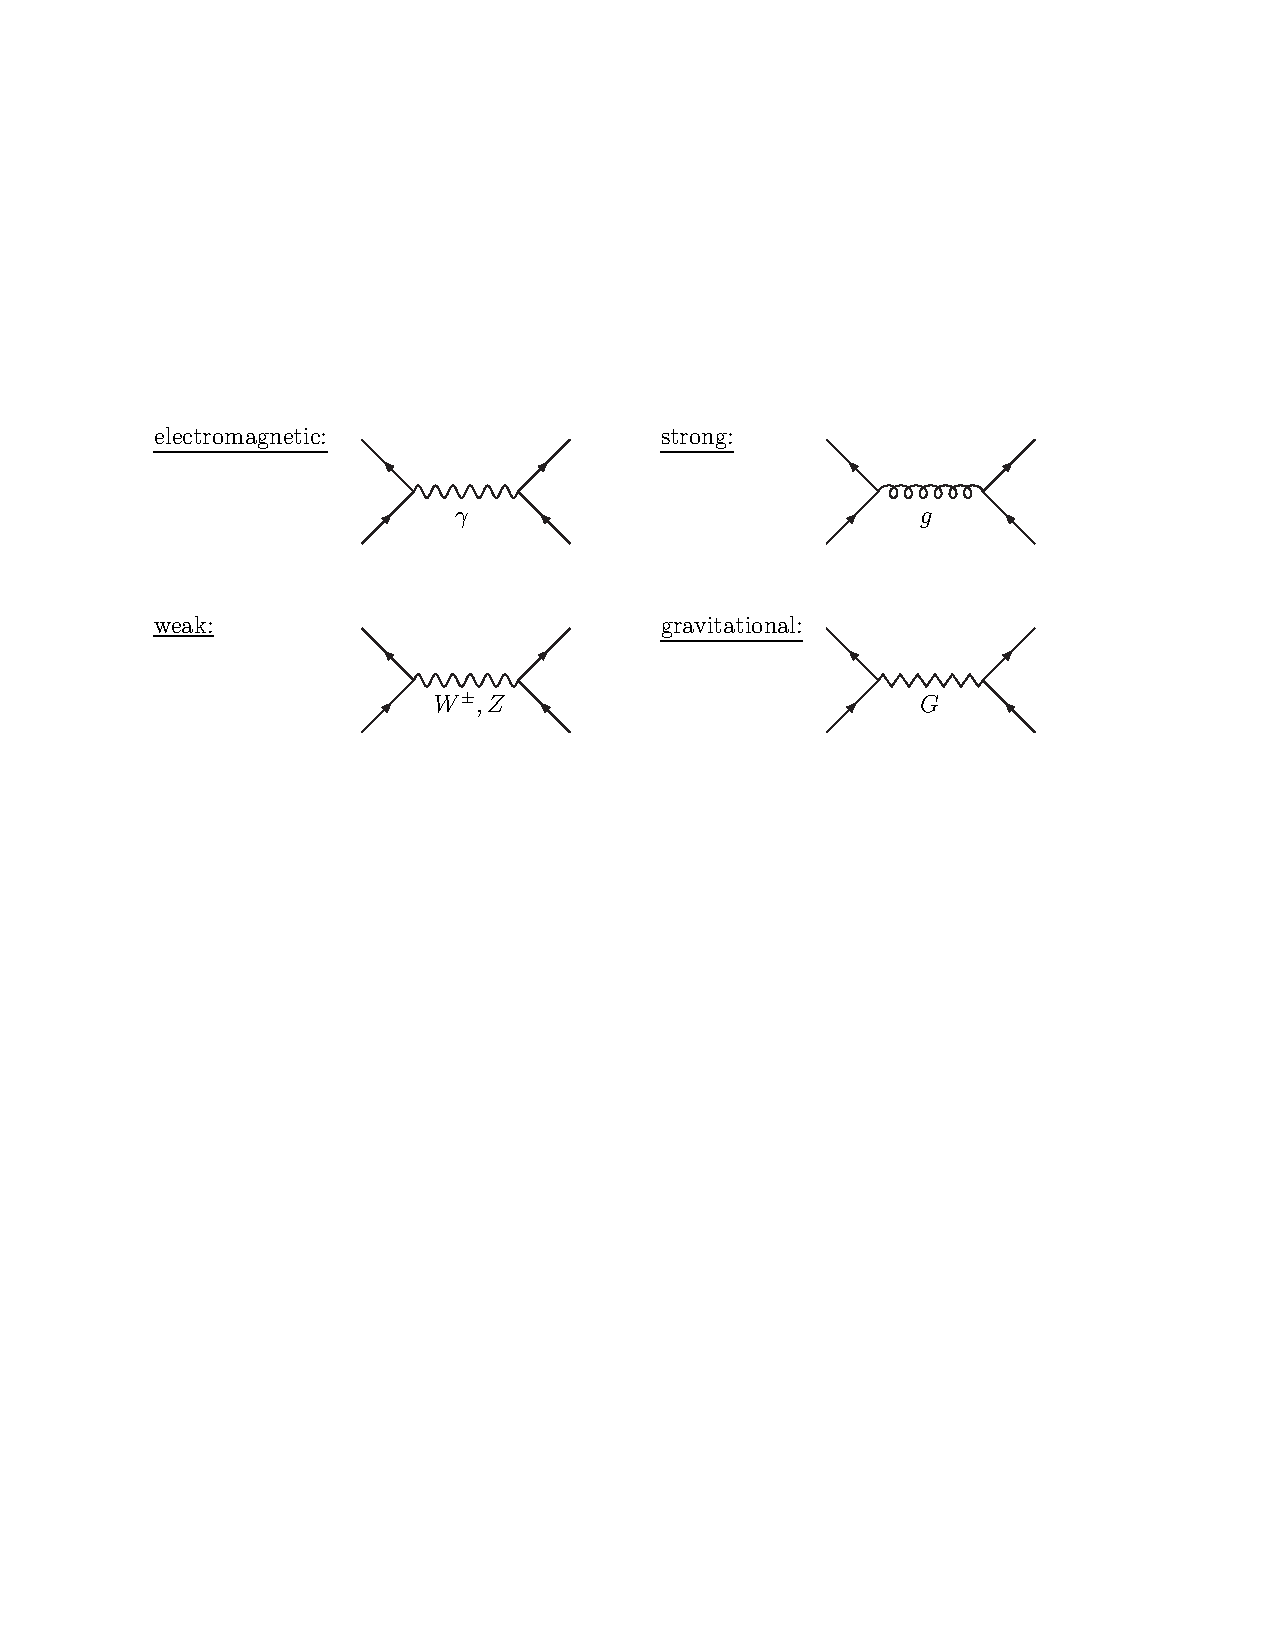
\includegraphics[width=0.75\textwidth]{theory/pics/SM_forces.pdf}
		\end{tabular}
		\caption{The four fundamental forces in nature as described by the Standard Model.}
		\label{fig:SM_forces}
	\end{figure}

\subsection{Interactions}

The interactions are mediated by bosons. They are the quanta of the gauge fields, and couple to the corresponding charges. The interactions are described by symmetry transformations U of the group SU(n). They are unitary (UU† = 1) and special (det(U) = 1). An operator


-----------------------------
	
The second component are the four different forces acting between the leptons and quarks. The electromagnetic and weak forces are unified in the Standard Model. The fields associated with these forces, as well as the fields associated with the strong force, are spin-1 fields, describing the photon \ensuremath{\gamma}, the electroweak gauge bosons \W and \Z, and the gluons g. The interactions of the force fields with the fermionic constituents of matter as well as their self-interactions are described by Abelian and non-Abelian \ensuremath{SU(3) \times SU(2) \times U(1)} gauge theories. The experimental exploration of these fundamental gauge symmetries is far advanced in the sector of lepton/quark-gauge boson interactions, yet much less is known so far from experiment about the self-interactions of the force fields. The gravitational interaction is mediated by a spin-2 field, describing the graviton G, with a character quite different from spin-1 gauge fields. The gravity sector is attached ad hoc to the other sectors of the Standard Model, not properly formulated yet as a quantum phenomenon. Figure \ref{fig:SM_forces} shows the four fundamental forces in nature as described by the Standard Model.



\begin{figure}[tbh!]
	\centering
	\begin{tabular}{cc}
		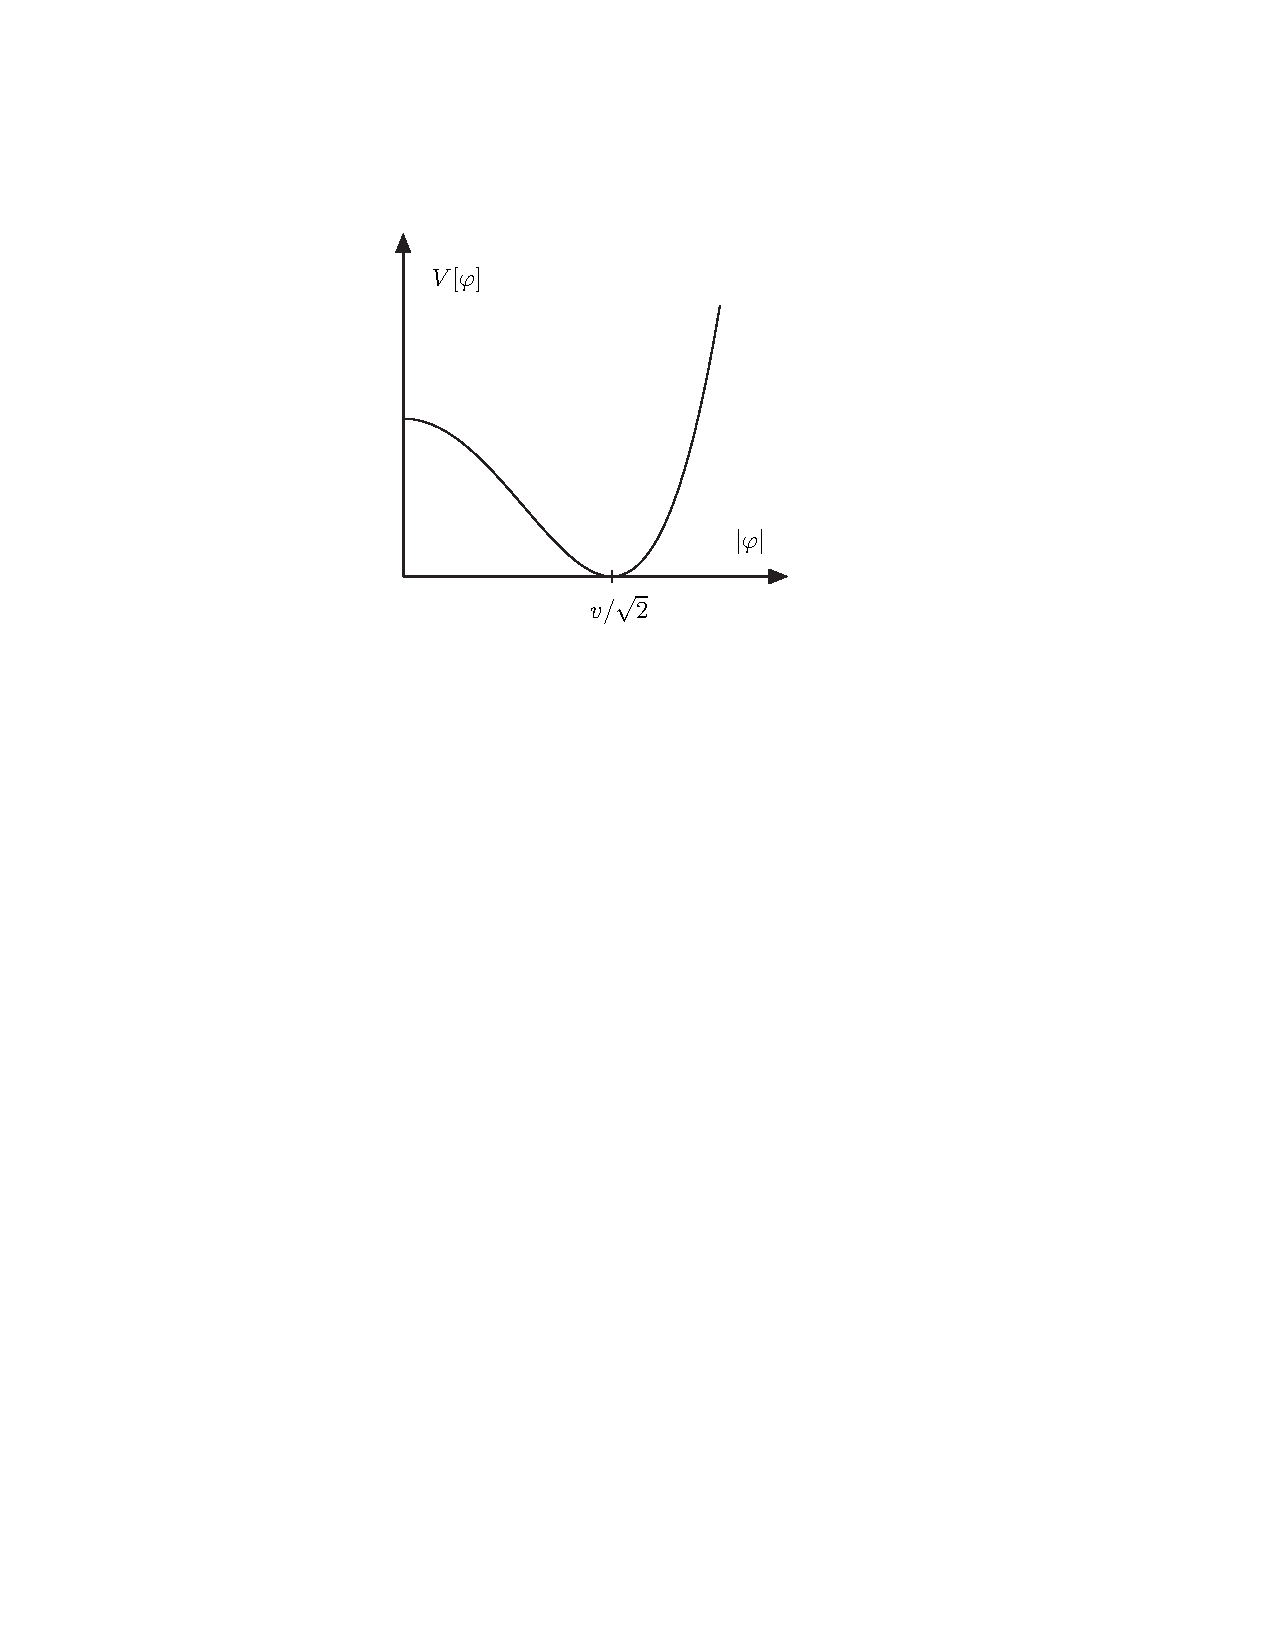
\includegraphics[width=0.75\textwidth]{theory/pics/higgs_potential.pdf}
	\end{tabular}
	\caption{The Higgs potential of the Standard Model.}
	\label{fig:higgs_potential}
\end{figure}


\subsection{The Higgs Mechanism}
\label{higgs_mechanism}

The starting point is the promotion from a global gauge transformation to the minimal to a point-dependent gauge transformation to the minimal Lagrangian . This requires in addition to the starting complex scalar field also a vectorial field $A_{\mu}$ analog to the electromagnetic field. The resulting Lagrangian is:

\begin{equation}
\mathcal{L} = (D_{\mu}\phi)^{\dagger} D^{\mu}\phi - V (\phi) - \dfrac{1}{4}F_{\mu\nu}F^{\mu\nu}\
\label{eq::lagrangian_min}
\end{equation}
\begin{equation}
V(\phi)=\mu^{2}\phi^{\dagger}\phi+\lambda(\phi^{\dagger}\phi)^{2} -\epsilon\phi^{\dagger} -\epsilon^{*}\phi
\end{equation}

\begin{equation}
D^{\mu} = \partial^{\mu} - ieA^{\mu}
\end{equation}

\begin{equation}
F^{\mu\nu} =\partial^{\nu}A^{\mu} - \partial^{\mu}A^{\nu}
\end{equation}

where $\epsilon \rightarrow 0$, $\mathcal{L}$ is invariant under gauge transformations:

\begin{equation}
\phi(x) \rightarrow e^{i\alpha(x)}\phi(x); \phi(x)^{\dagger} \rightarrow e ^{-i\alpha(x)}\phi(x)^{dagger}
\end{equation}

\begin{equation}
A^{\mu} \rightarrow A^{\mu} + \dfrac{1}{e}\partial^{\mu}\alpha(x)
\label{eq::a_tranform}
\end{equation}

Where $\alpha(x)$ is an arbitrary function of x and $e$ is a new coupling constant, identical to the electrical charge in case $A_{\mu}$ is identified as the electromagnetic field. In order to obtain a stable theory $\lambda > 0$, however $\mu^{2}$ can have two cases depending on the sign choice:
 
1. $\mu^{2} > 0$. The energy minimum is at $\phi = 0$ and $A_{\mu} = 0$. The resulting theory consists of:

\begin{enumerate}
	\item a charged particle and its anti-partner, both with mass $\mu^{2} \neq 0$;
	\item a massless particle with spin 0, similar to the photon.
\end{enumerate}

For small values of $\lambda$ and $e$ the Lagrangian describes the interactions between scalar particles with the electromagnetic field (trough the coupling constant $e$) and their self-interactions (through the couping constant $\lambda$).

2. $\mu^{2} < 0$. The energy minimum is at $A_{\mu} = 0$, so in  case $\epsilon \rightarrow 0$:

\begin{equation}
V(\bar{\phi})=min ; \quad \bar{\phi}=\eta= 2\lambda +O(\epsilon)
\end{equation}
 
 in order to study the  variations around the minimum $\phi$ is defined as:

\begin{equation}
 \phi=\eta + \dfrac{\sigma_{1}(x) + i\sigma_{2}(x)}{\sqrt{2}} 
\end{equation}

and is used into the minimal Lagrangian \ref{eq::lagrangian_min}.

The particle masses spectrum is obtained from the fields $\sigma_{i}$ and $A_{\mu}$ quadratic terms. In addition, for $\alpha \rightarrow 0$, $\phi$ transforms as:

\begin{equation}
\phi \rightarrow \phi + i\alpha\phi = \eta + \dfrac{\sigma_{1}(x) + i\sigma_{2}(x)}{\sqrt{2}} + i\eta\alpha(x)
\end{equation}

or rather:

\begin{equation}
\sigma_{1}(x) \rightarrow \sigma^{\prime}_{1}(x) = σ_{1}(x); \quad \sigma_{2}(x) \rightarrow \sigma^{\prime}_{2}(x) = \sigma_{2}(x) + \sqrt{2}\eta\alpha(x)
\end{equation}

$A_{\mu}$ transforms following \ref{eq::a_tranform}. The $\sigma_{2}$ field non-homogeneously transforms by the addition of an $\alpha$ term, arbitrary function of $x$. In case of the given $\sigma_{i}(x)$ and $A_{\mu}$ where:

\begin{equation}
\alpha(x) = -\dfrac{σ\sigma_{2}(x)}{\sqrt{2}\eta}
\end{equation}

resulting in:

\begin{equation}
\sigma^{\prime}_{2}(x) = 0
\label{eq::unitary_gauge}
\end{equation}

the $\sigma_{2}$ filed can be crossed out in case of a gauge symmetry. The gauge identified by \ref{eq::unitary_gauge} is commonly known as unitary gauge.

\begin{figure}[tbh!]
	\centering
	
	\begin{tabular}{cc}
		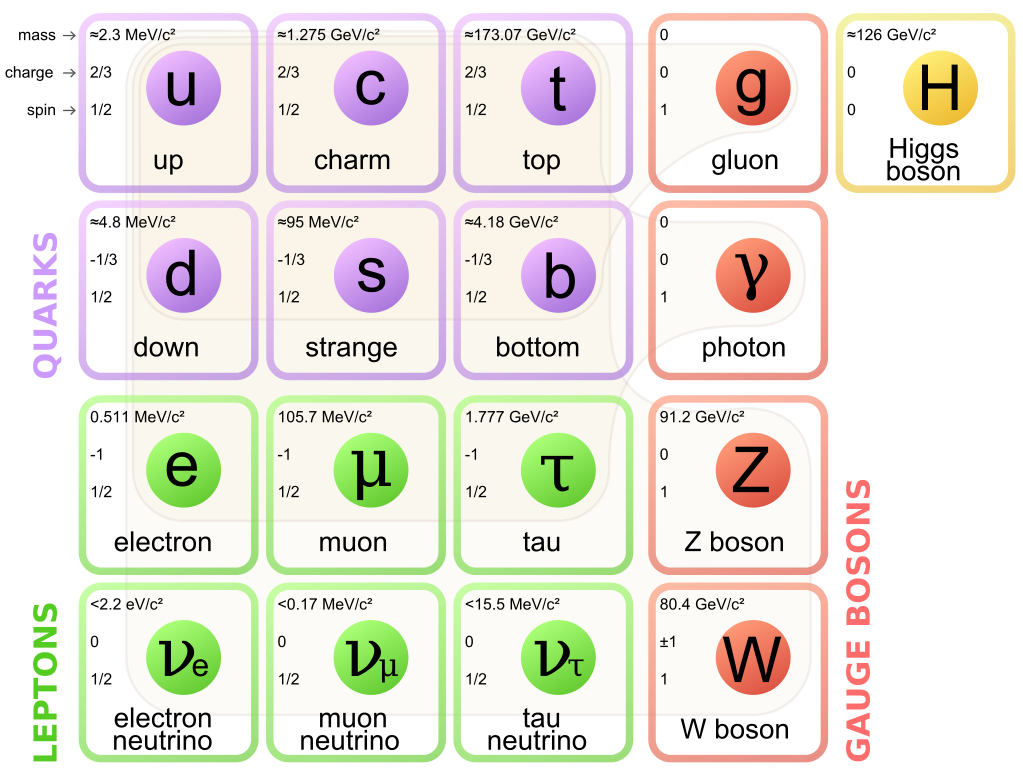
\includegraphics[width=0.75\textwidth]{theory/pics/SM_particles.png}
	\end{tabular}
	\caption{The Standard Model of elementary particles consists of  12 fundamental fermions and 4 fundamental bosons. Brown loops indicate which bosons (red) couple to which fermions (purple and green).}
	\label{fig:SM_particles}
\end{figure}

\begin{figure}[tbh!]
	\centering
	\begin{tabular}{cc}
		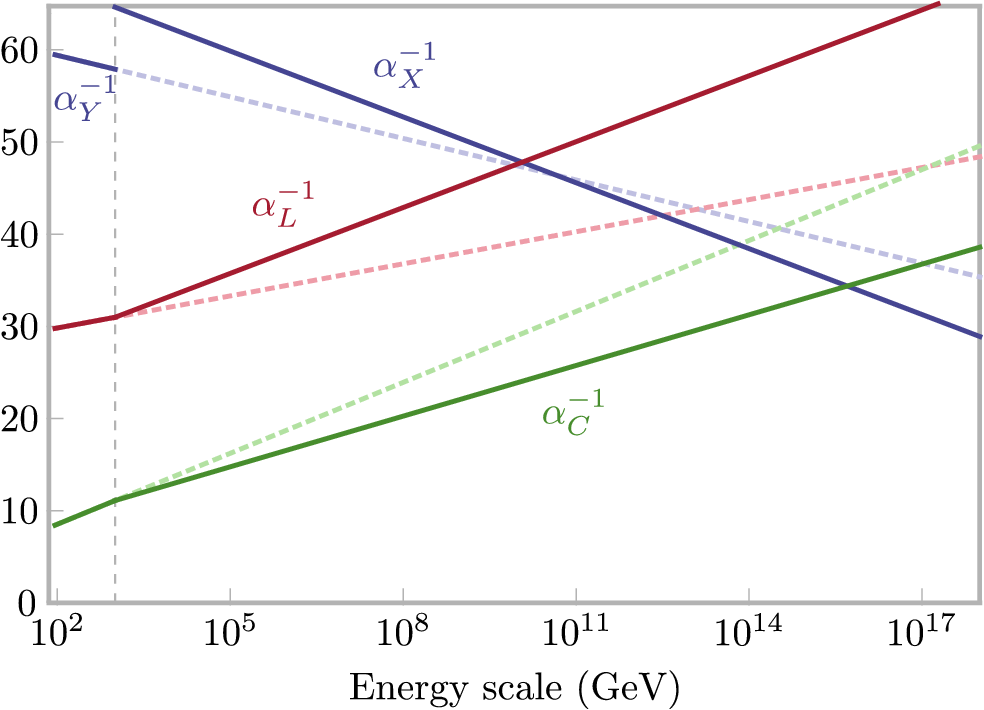
\includegraphics[width=0.75\textwidth]{theory/pics/gauge_unification.png}
	\end{tabular}
	\caption{Running of the gauge coupling constants in the SM (dashed lines) and in the model in Ref.~\cite{PhysRevD.90.013005} (solid lines). Here the $M_{331}$ scale is set to 11~TeV}
	\label{fig:gauge_unification}
\end{figure}

\subsection{The bosonic masses}

The starting point is a theory based on the $SU(2)_{L} \oplus U(1)_{Y}$ symmetry:

\begin{equation}
\mathcal{L}_{eW} = \bar{l}i\gamma^{\mu} D_{\mu}l + \bar{e}_{R}i\gamma^{\mu}D_{\mu}e_{R} − \dfrac{1}{4}[W_{\mu\nu}W^{\mu\nu} +B_{\mu\nu}B^{\mu\nu}]
\label{eq::lagrangian_ew}
\end{equation}

with the leptonic fields defined as:

\begin{equation}
\binom{(\nu_{e})_{L}}{e_{L}}_{Y=−2} ; \quad (e_{R})_{Y=−2}
\label{eq::fields_scheme}
\end{equation}

and the covariant derivatives and tensors defined as:

\begin{equation}
D_{\mu}l = [\partial_{\mu} + igW_{\mu} \dfrac{\tau}{2}  + ig^{\prime}(-\dfrac{1}{2})B_{\mu}]l 
\end{equation}

\begin{equation}
D_{\mu}e_{R} = [\partial_{\mu} + ig^{\prime}(-1)B_{\mu}]e_{R}
\end{equation}

\begin{equation}
W_{\mu\nu} =\partial_{\nu}W_{\mu} - \partial_{\mu}W_{\nu} 
\end{equation}

\begin{equation}
B_{\mu\nu} =\partial_{\nu}B_{\mu} - \partial_{\mu}B_{\nu} 
\end{equation}

At this stage the theory describes massless fermions and vectorial fields. The introduction of a scalar field triggers a symmetry breaking while keeping the electromagnetism gauge still intact:

\begin{equation}
SU(2)_{L} \oplus U(1)_{Y} \rightarrow U(1)_{em}
\end{equation}

The optimal choice in order to generate the electron and quarks mass is to choose a $SU(2)_{L}$ doublet with $Y = +1$: 

\begin{equation}
\phi = \binom{(\phi{+})_{L}}{\phi^{0}}_{Y=+1}
\label{eq::su2_doublet}
\end{equation}

\begin{equation}
D_{\mu}\phi = [\partial_{\mu} + igW_{\mu} \dfrac{\tau}{2}  + ig^{\prime}(+\dfrac{1}{2})B_{\mu}]\phi 
\end{equation}


with the addition of the fully symmetric Higgs doublet to \ref{eq::lagrangian_ew} the total Lagrangian becomes:

\begin{equation}
\mathcal{L}_{tot} = \mathcal{L}_{eW} + \mathcal{L}_{\phi W}
\end{equation}

where:

\begin{equation}
\mathcal{L}_{\phi W} = (D_{\mu}\phi)^{\dagger} (^{\mu}\phi) - V (\phi);
\label{eq::lagrangian_phiW}
\end{equation}

\begin{equation}
V(\phi) = \mu^{2}\phi^{\dagger}\phi + \lambda(\phi^{\dagger}\phi)^{2}
\end{equation}

Following the example shown in Section \ref{higgs_mechanism}, $\phi$ can gain a vacuum expectation term, breaking the symmetry:

\begin{equation}
 \bar{\phi}= < 0|\phi|0 > = \binom{0}{\eta}
 \label{eq::vacuum_expectation}
\end{equation}

where:

\begin{equation}
\eta = \sqrt{\dfrac{-\mu^{2}}{2\lambda}}
\label{eq::eta_value}
\end{equation}

In the \ref{eq::su2_doublet} doublet the electric charge is represented as:

\begin{equation}
Q = 
\begin{pmatrix}
+1 & 0 \\
0 & 0 \\
\end{pmatrix}
\end{equation}

so that the field minimum is invariant under phase transformations associated to $U_{em}(1)$:

\begin{equation}
e^{i\alpha Q} \bar{\phi} = 
\begin{pmatrix}
e^{i\alpha} & 0 \\
0 & 1 \\ 
\end{pmatrix}
\binom{0}{\eta}
= \bar{\phi}
\end{equation}

The symmetry breaking given by $\bar{\phi} \neq 0$ gives the scheme \ref{eq::fields_scheme}.
In order to correctly identify all the particles qa definition of the unitary gauge conditions is mandatory. Knowing that every two-dimensional spinor can transform to a spinor with only a real lower component through a point-dependent gauge transformation. Therefore a given $\phi(x)$
can be defined as:

\begin{equation}
\phi(x) = U(x) \binom{0}{\rho(x)}
\end{equation}

with $\rho(x)$ real and $U(x)$ as matrix of $ SU(2)_{L} \oplus U(1)_{Y}$. 

In the previously defined unitary gauge the Lagrangian \ref{eq::lagrangian_phiW} becomes:

\begin{equation}
\begin{array}{r c l}
\mathcal{L}_{\phi W}&=&\dfrac{1}{2} \partial_{\mu} \sigma \partial^{\mu} \sigma - V \left[ \eta + \dfrac{\sigma(x)}{\sqrt{2}}\right] + g^{2} W_{\mu}^{i}(W^{j})^{\mu} \left[ \bar{\phi} \dfrac{\tau_{i}\tau_{j}}{4}\bar{\phi}\right] +\\
&+&(g^{\prime})^{2} \dfrac{1}{4}\eta^{2} B_{\mu} B^{\mu} + 2 gg^{\prime} W^{3}_{\mu} B^{\mu} \left[ \bar{\phi} \dfrac{\tau_{3}}{4} \bar{\phi} \right]
\end{array}
\end{equation}

By using  \ref{eq::vacuum_expectation} and \ref{eq::eta_value} along with the Pauli's matrixes properties:

\begin{equation}
\begin{array}{c}
 W_{\mu}^{i}(W^{j})^{\mu} \left[ \bar{\phi} \dfrac{\tau_{i}\tau_{j}}{4}\bar{\phi}\right] = \frac{1}{4}\eta^{2} W_{\mu}W^{\mu} \\

 W^{3}_{\mu} B^{\mu} \left[ \bar{\phi} \dfrac{\tau_{3}}{4} \bar{\phi} \right] = - \dfrac{1}{4} \eta^{2} W^{3}_{\mu}B^{\mu}
 \end{array}
\end{equation}

from the quadratic terms is possible to get the masses value:

\begin{equation}
\begin{array}{c}
W_{\mu}^{i}(W^{j})^{\mu} \left[ \bar{\phi} \dfrac{\tau_{i}\tau_{j}}{4}\bar{\phi}\right] = \frac{1}{4}\eta^{2} W_{\mu}W^{\mu} \\

W^{3}_{\mu} B^{\mu} \left[ \bar{\phi} \dfrac{\tau_{3}}{4} \bar{\phi} \right] = - \dfrac{1}{4} \eta^{2} W^{3}_{\mu}B^{\mu}
\end{array}
\end{equation}

which becomes:

\begin{equation}
\begin{array}{c}
M^{2}  = \dfrac{1}{2} g^{2} \eta^{2}\\
M_{0}^{2}  = \dfrac{1}{2} (g^{\prime})^{2} \eta^{2}\\
M_{03}^{2}  = -\dfrac{1}{2} gg^{\prime} \eta^{2}
\end{array}
\end{equation}

therefore:

\begin{equation}
\mathcal{M} =  \dfrac{1}{2} \eta^{2}
\begin{pmatrix}
 g^{2} & -gg^{\prime} \\
-gg^{\prime} & (g^{\prime})^{2} \\
\end{pmatrix}
\end{equation}

in order to allow the existence of a massless photon $det(\mathcal{M}) = 0$. Knowing that the vacuum configuration in invariant to gauge transformation associated to the electric charge is possible to introduce the massive field $Z_{\mu}$ and the electric field $A_{\mu}$ so that:

\begin{equation}
\begin{array}{c}
Z_{\mu} = cos\theta W^{3}_{\mu} - sin\theta B_{\mu}\\
A_{\mu} = sin\theta W^{3}_{\mu} - cos\theta B_{\mu}

\end{array}
\end{equation}

with $\theta$ knows as the electroweak mixing angle. 

\clearpage

\subsection{Limitations}

\todo{Total Rework}

Although the Standard Model is very successful in describing physics at the electroweak scale, a few questions remain:

\begin{itemize}
	\item Gravity: The Standard Model does not include gravity and already for this reason alone, it cannot be a complete description of nature.
	\item No Electrostrong Unification: The hope of physics in the end is to unify all forces, but while the strong force is well represented by the SU(3), it is not unified with the other forces like it is the case for the electromagnetic and the weak force.
	\item Dark Matter: Astrophysical observations indicate a much greater accumulation of matter in the visible universe than can be explained by baryonic matter [13]. This “dark matter” cannot be explained by neutrinos, which could form only a small fraction of it. The “Modified Newtonian Dynamics” (MOND) [14] was developed in order to explain this excess within the existing theories. It was very successful, especially in explaining the measurement of galaxy rotation curves [15], until the bullet cluster [16] was discovered. Being actually two clusters passing each other, the bullet cluster shows a discrepancy between the center of the masses detected by direct observation and the center of the masses detected by gravitational lensing. This cannot be explained by MOND alone.
	\item WW Scattering: In the Standard Model, the four-vector-boson interaction becomes divergent with rising energy. If the Higgs mechanism turns out to be realized, a new term due to interactions of the vector-bosons with the Higgs is introduced, which cancels out this divergence. But this will only work, if the higgs mass is of the order of 100 GeV, and the WW scattering problem turns into the “fine-tuning” problem.
	\item Neutrino Masses: In the original Standard Model, neutrinos are set to be massless. Experiments showed that neutrinos indeed have non-zero masses [17]. In case of a sterile Dirac neutrino5, the Standard Model can be extended to include massive neutrinos. If it turns out that neutrinos are Majorana particles6, new physics beyond the Standard Model has to be introduced to explain the tiny masses of the neutrinos.
	\item Hierarchy Problem: In the Standard Model, the quantum corrections to the Higgs mass are quadratically divergent. If the Standard Model is assumed to be valid up to the Planck scale7, these corrections are huge compared to the physical Higgs mass.
\end{itemize}

\section{Supersymmetry}

Supersymmetry is one of the most intriguing and fundamental concepts in modern theoretical particle physics. It arises naturally from the combination of the two cornerstones of 20th century physics: quantum mechanics and relativity. Supersymmetry is the unique symmetry that relates the two fundamental kinds of particles: bosons, which act as the carriers of forces, and fermions, which act as the constituents of matter. Supersymmetry transformations are in a sense like the square roots of the coordinate system transformations in special relativity, and consequently supersymmetric quantum field theories have very special, improved properties, compared to ordinary relativistic quantum field theories. If supersymmetry is realized in nature, every fermion in the SM must have a bosonic partner particle and vice versa. No such superpartner particle has been observed so far but there are more and more indications that these particles might show up at the LHC experiments.


\begin{figure}[tbh!]
	\centering
	\begin{tabular}{cc}
		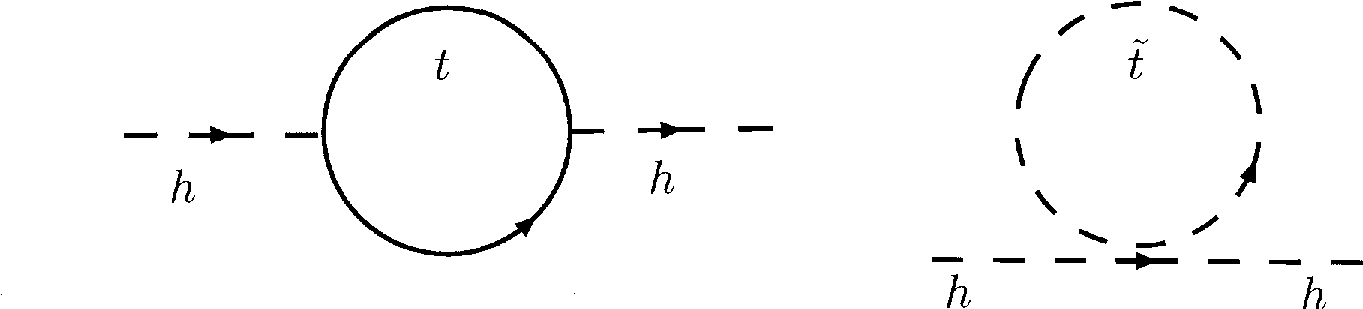
\includegraphics[width=0.75\textwidth]{theory/pics/higgs_loop.png}
	\end{tabular}
	\caption{In SUSY, the correction to Higgs mass by the top quark (L) is inherently cancelled by the contribution from the top quark's supersymmetric partner, the stop (R).}
	\label{fig:higgs_loop}
\end{figure}

\subsection{Motivations}

\subsection{The MSSM}

\begin{figure}[tbh!]
	\centering
	\begin{tabular}{cc}
		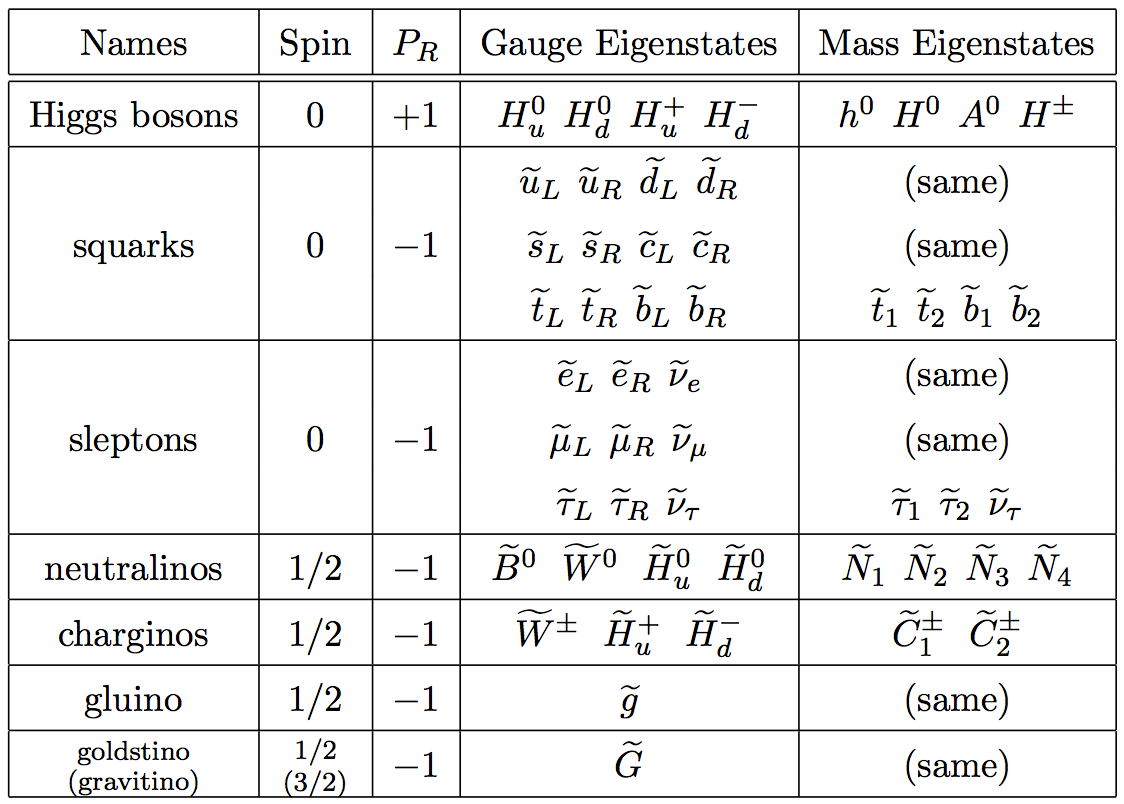
\includegraphics[width=0.75\textwidth]{theory/pics/SUSY_particles_table.png}
	\end{tabular}
	\caption{SUSY particles in MSSM~\protect\cite{Martin:1997ns}}
	\label{fig:SUSY_particles_table}
\end{figure}

\begin{figure}[tbh!]
	\centering
	\begin{tabular}{cc}
		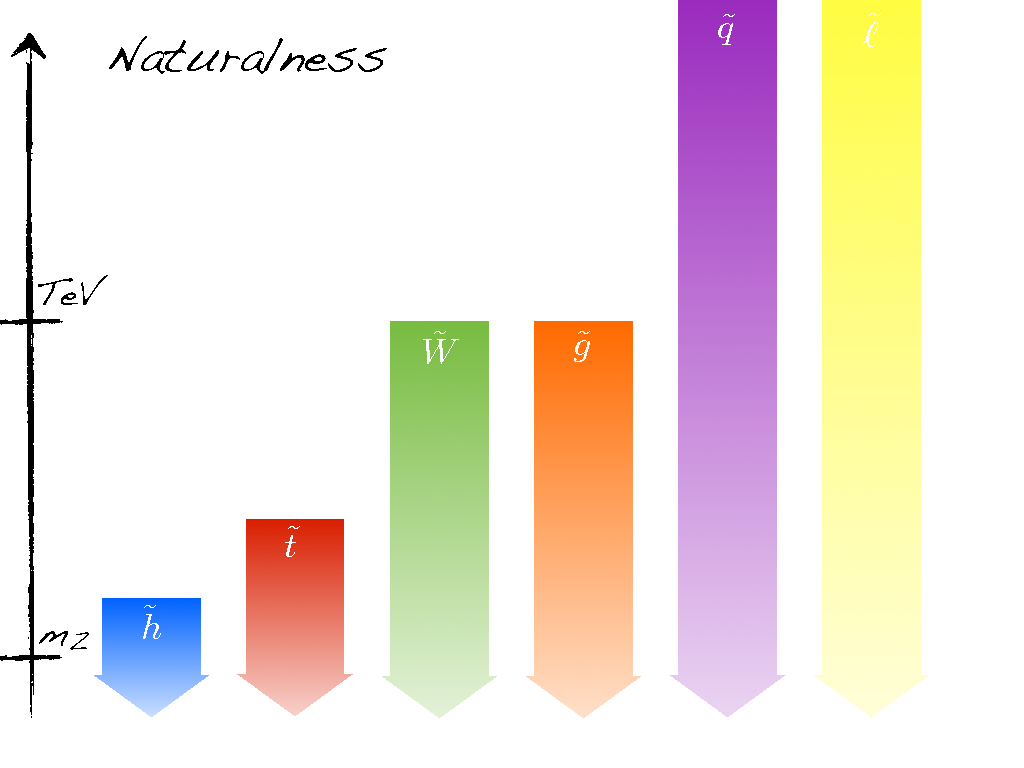
\includegraphics[width=0.75\textwidth]{theory/pics/SUSY_naturalness.png}
	\end{tabular}
	\caption{Cartoon illustration of the mass scales for various sparticles dictated solely by electroweak naturalness with sensitivity parameter $\Delta \lesssim 10$.}
	\label{fig:SUSY_naturalness}
\end{figure}




\subsection{SUSY Signatures at the LHC}

\cleardoublepage

\chapter{The Experimental Setup}
\label{sec:detector}


\section{The Large Hadron Collider}

The Large Hadron Collider (LHC) is the world's largest and most powerful particle collider, the largest, most complex experimental facility ever built, and the largest single machine in the world.[1] It was built by the European Organization for Nuclear Research (CERN) between 1998 and 2008 in collaboration with over 10,000 scientists and engineers from over 100 countries, as well as hundreds of universities and laboratories. It lies in a tunnel 27 km in circumference, as deep as 175 m beneath the France–Switzerland border near Geneva, Switzerland, originally build for the Large Electron Positron Collider (LEP). 

\begin{figure}[tbh!]
	\centering
	\begin{tabular}{cc}
		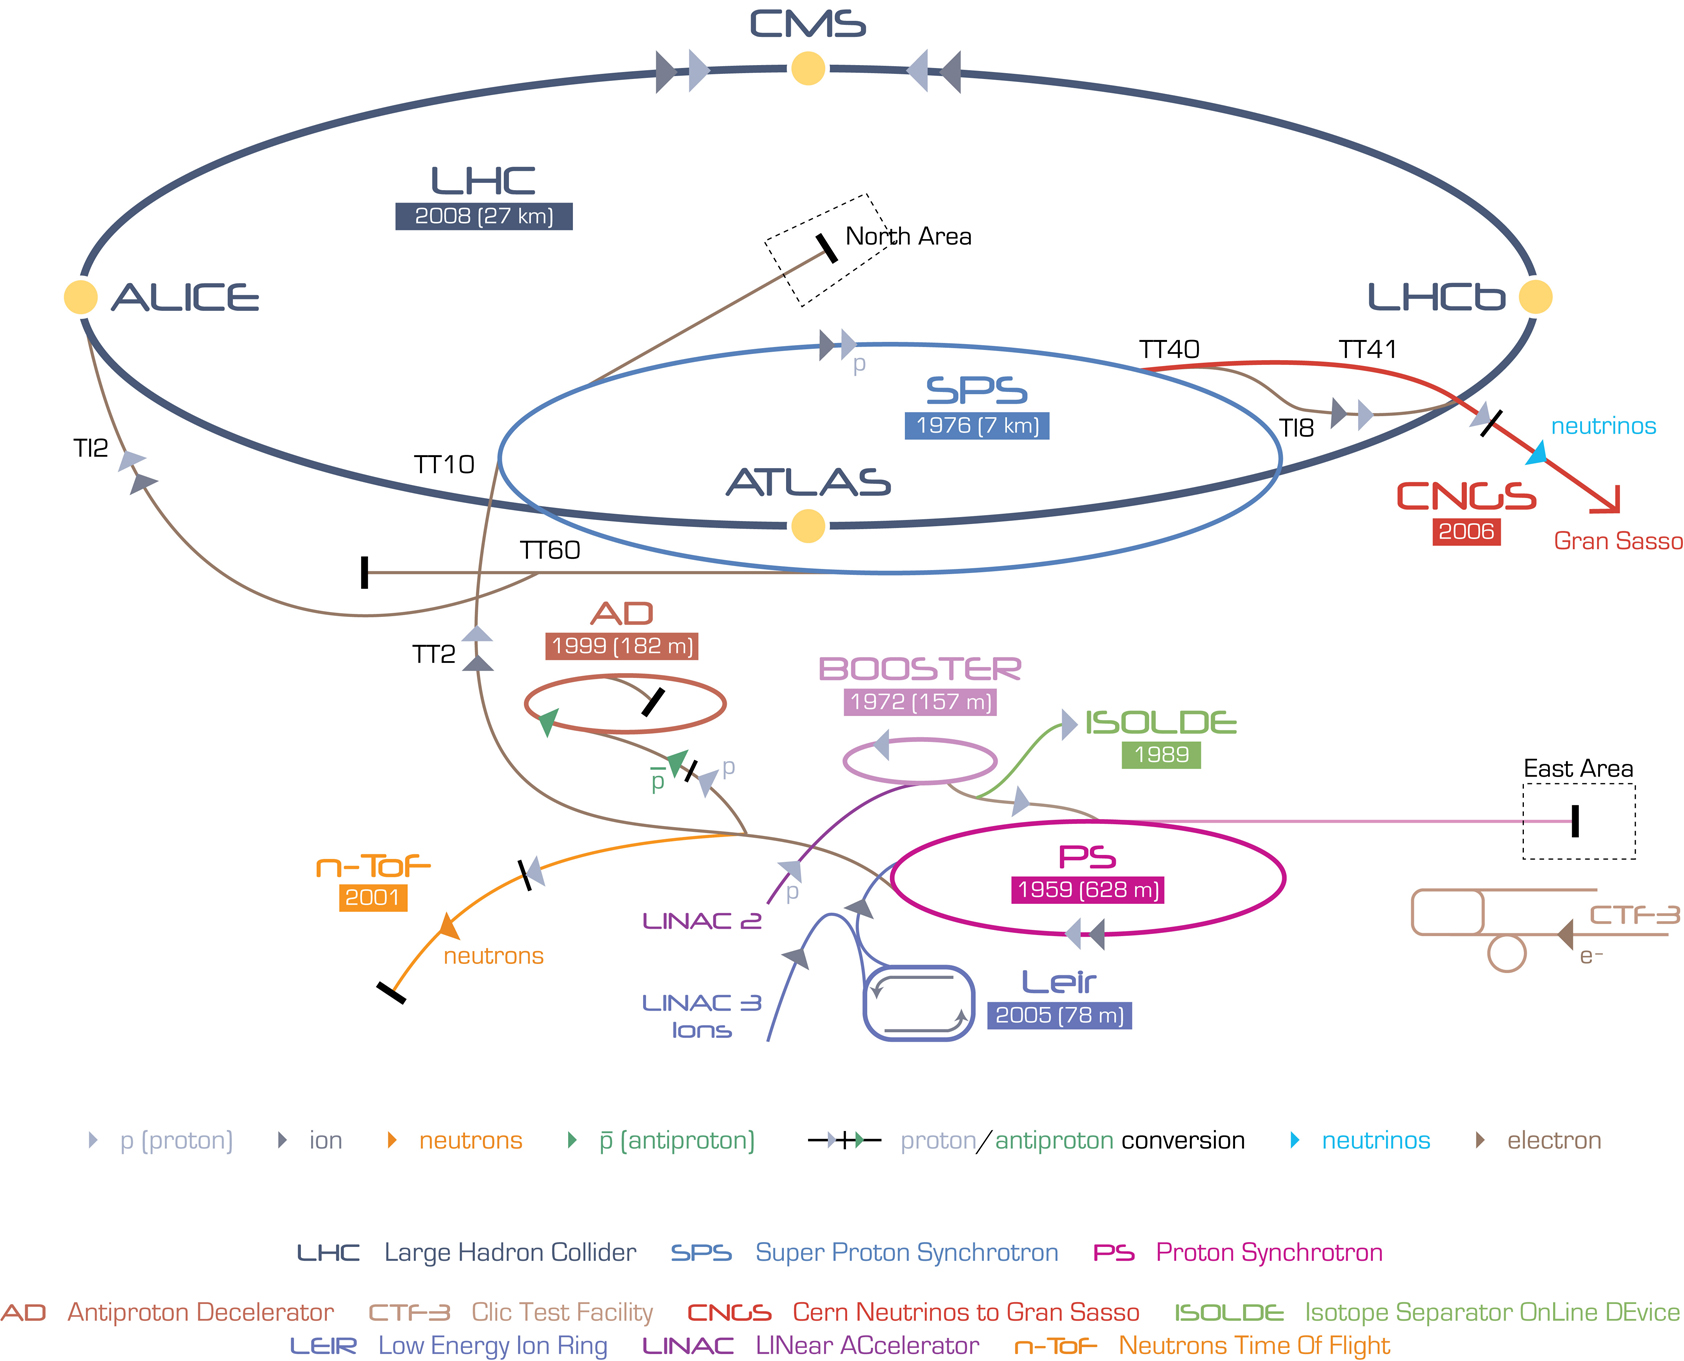
\includegraphics[width=0.75\textwidth]{detector/pics/CERN_complex.jpg}
	\end{tabular}
	\caption{Schematic view of the LHC with its four big experiments. Also shown are the pre-accelerators, as well as several other experiments operated at CERN.}
	\label{fig:CERN_complex}
\end{figure}

The Large Hadron Collider (LHC) is a proton-proton collider at the European OrganizItion for Nuclear Research (CERN)1, residing in the $26.7$ km tunnel originally build for the Large Electron Positron Collider (LEP).It consists of two rings with counter-rotating beams, being crossed at four interaction points. The proton beams are ramped up to the energy of 450 GeV by a chain of pre-accelerators, and are then injected into the LHC ring (Figure \ref{fig:CERN_complex}). LHC first official run started on March 2010 and last for almost 3 years with an initial energy per beam of 3.5 \tev (7 \tev in total), rising to 4 \tev per beam (8 \tev in total) in 2012. The shutdown in 2013 was followed by two years of technical upgrades after that the LHC restarted the run with a with a total beam energy of 13 \tev. The design luminosity of L is $10^{34} cm^{-2}s^{-1}$ has been reached in june 2016, with a bunch crossing every $25 ns$. Figure \ref{fig:LHC_xsec} shows the total cross section prospects for LHC in comparison with several Standard Model processes. In 2012 LHC delivered a total luminosity of 23.30 $fb^{-1}$ as shown on \ref{fig:lumi_2012}.

\begin{figure}[tbh!]
	\centering
	\begin{tabular}{cc}
		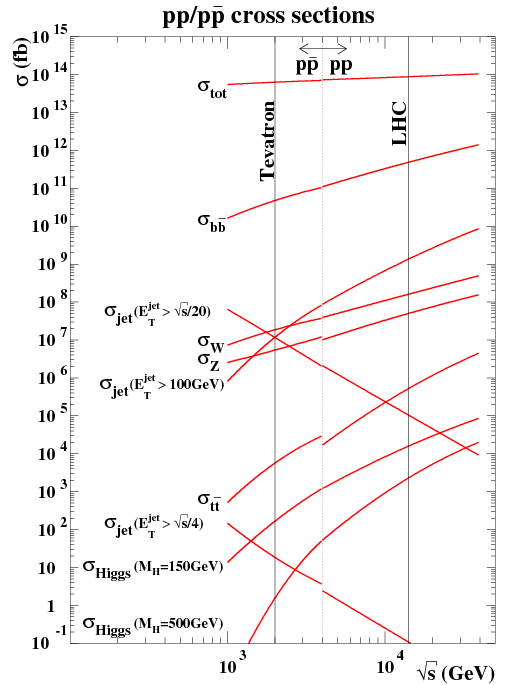
\includegraphics[width=0.75\textwidth]{detector/pics/LHC_xsec.png}
	\end{tabular}
	\caption{Production cross-sections for several representative processes at hadron colliders as a function of the machine center-of-mass energy}
	\label{fig:LHC_xsec}
\end{figure}


Several experiments are hosted at the LHC. ATLAS (A Toroidal Lhc ApparatuS) \cite{det::ATLAS} and CMS (Compact Muon Solenoid) \cite{Chatrchyan:2008zzk} are multi-purpose detectors, aiming at Standard Model physics including Higgs searches and physics beyond the Standard Model. LHCb \cite{det::LHCb} is dedicated to b-quark physics and the related problem of CP violation the matter-antimatter asymmetry in the universe. As the LHC can also be run in heavy ion (lead-lead) collision mode, one experiment, ALICE (A Large Ion Collider Experiment) \cite{det::ALICE}, focuses on strongly interacting matter and quark-gluon plasma. Finally, another two experiments, LHCf \cite{Adriani:2008zz} and TOTEM (TOTal Elastic and diffractive cross section Measurement) \cite{Anelli:2008zza} are designed to study the total proton-proton interaction cross-section. The site for each of the previously mentioned experiments is shown in Figure \ref{fig:CERN_complex}. 

\begin{figure}[tbh!]
	\centering
	\begin{tabular}{cc}
		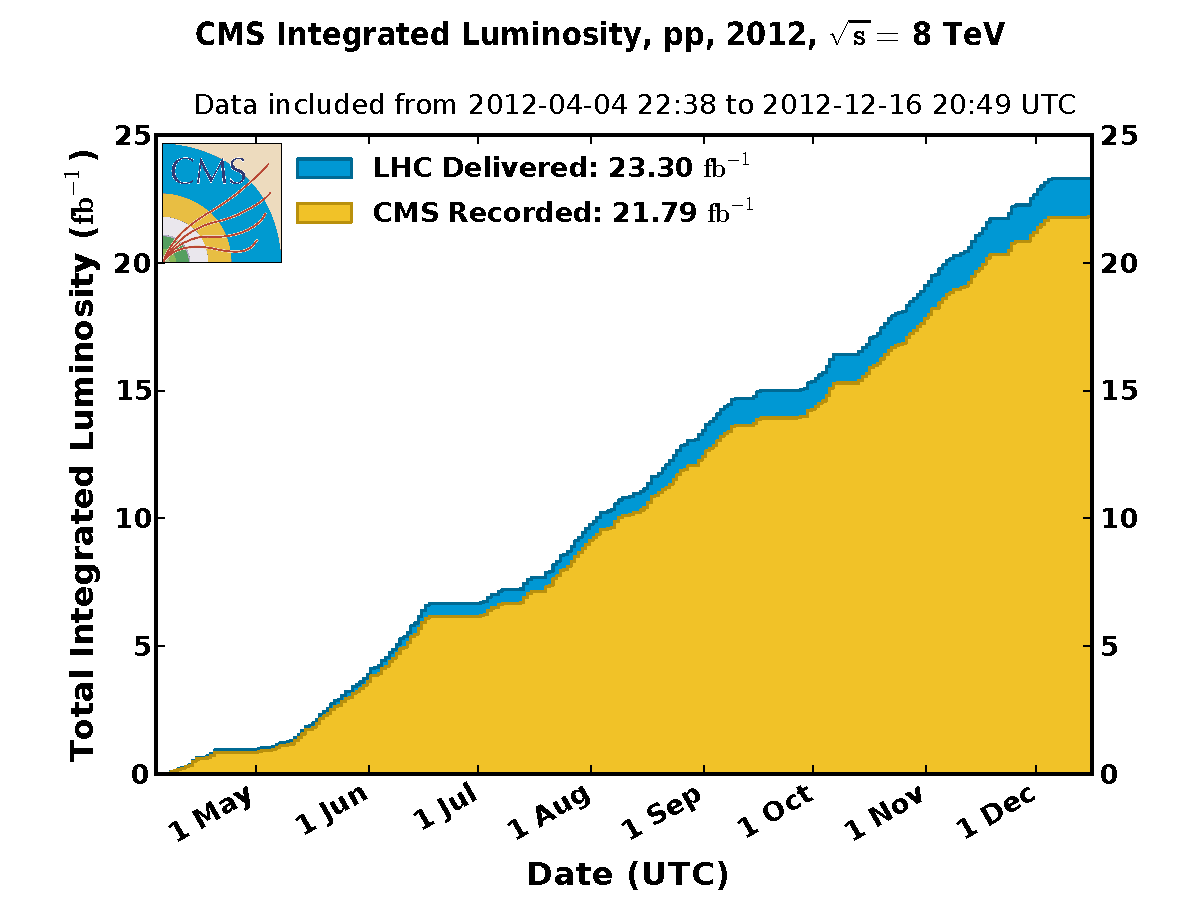
\includegraphics[width=0.75\textwidth]{detector/pics/int_lumi_per_day_cumulative_pp_2012.pdf}
	\end{tabular}
	\caption{Cumulative luminosity versus day delivered to (blue), and recorded by CMS (orange) during stable beams and for p-p collisions at 8 TeV centre-of-mass energy in 2012. The delivered luminosity accounts for the luminosity delivered from the start of stable beams until the LHC requests CMS to turn off the sensitive detectors to allow a beam dump or beam studies. Given is the luminosity as determined from counting rates measured by the luminosity detectors. These detectors have been calibrated with the use of the van-der-Meer beam-separation method, where the two beams are scanned against each other in the horizontal and vertical planes to measure their overlap function.}
	\label{fig:lumi_2012}
\end{figure}

\clearpage

\section{The CMS Experiment}

The Compact Muon Solenoid is a "general purpose" experiment placed at Point 5 along the LHC ring. The experiment has a cylindrical geometry and is divided in two main sections: the lateral section, called Barrel and the remaining ones called Endcaps (Figure \ref{fig:CMS_apparatus}).   
CMS was designed to fulfill the following important research tasks:
\begin{enumerate}
	\item Search for the Higgs Boson
	\item Search for physics beyond the standard model
\end{enumerate}
those tasks combined with the LHC design specifications require a detector with the following characteristics:
\begin{itemize}
	\item High granularity and response;
	\item High radiation damage resistance;
	\item Good performances in the reconstruction of the $\mu$ particle charge, momentum and invariant mass;
	\item Good $\tau$ particle and jets reconstruction efficiency;
	\item High resolution on the combined reconstruction of electrons and photons;
	\item Great phase-space coverage $|\eta| < 5$;
	\item Good resolution in the missing transverse energy reconstruction.
\end{itemize} 

The CMS detector has a $24 m$ length and a $14.6 m$ diameter for a total wight of $14500 t$. The experiment is made of several sub-detectors placed concentrically around the interaction point, each one providing complementary measurements (Figure \ref{fig:CMS_slice}). Particles coming from the interaction point first go through the tracking system witch measures the position of charged particles hitting its layers. The calorimeters are places right outside the tracking system and are capable of measuring the particles energy deposits. The Electromagnetic Calorimeter (ECAL) measure the energy of electrons and photons, the Hadronic Calorimeter (HCAL) measures the energy of all fermions containing quarks.

The most important section in the detector is the high magnetic field which allows the measurement of high momentum charged particles with high precision. Measurements with high resolution standards requires high magnetic fields, therefore the choice to use superconducting technology for the magnets. All previously introduced sub-detectors are contained inside the solenoid superconducting magnet. All particles except for $\mu$ and low interacting ones get contained by the calorimeters and the magnetic return yoke. Outside the magnet there are the muon chambers witch identify $\mu$ particles and measure their momentum.

\begin{figure}[tbh!]
	\centering
	\begin{tabular}{cc}
		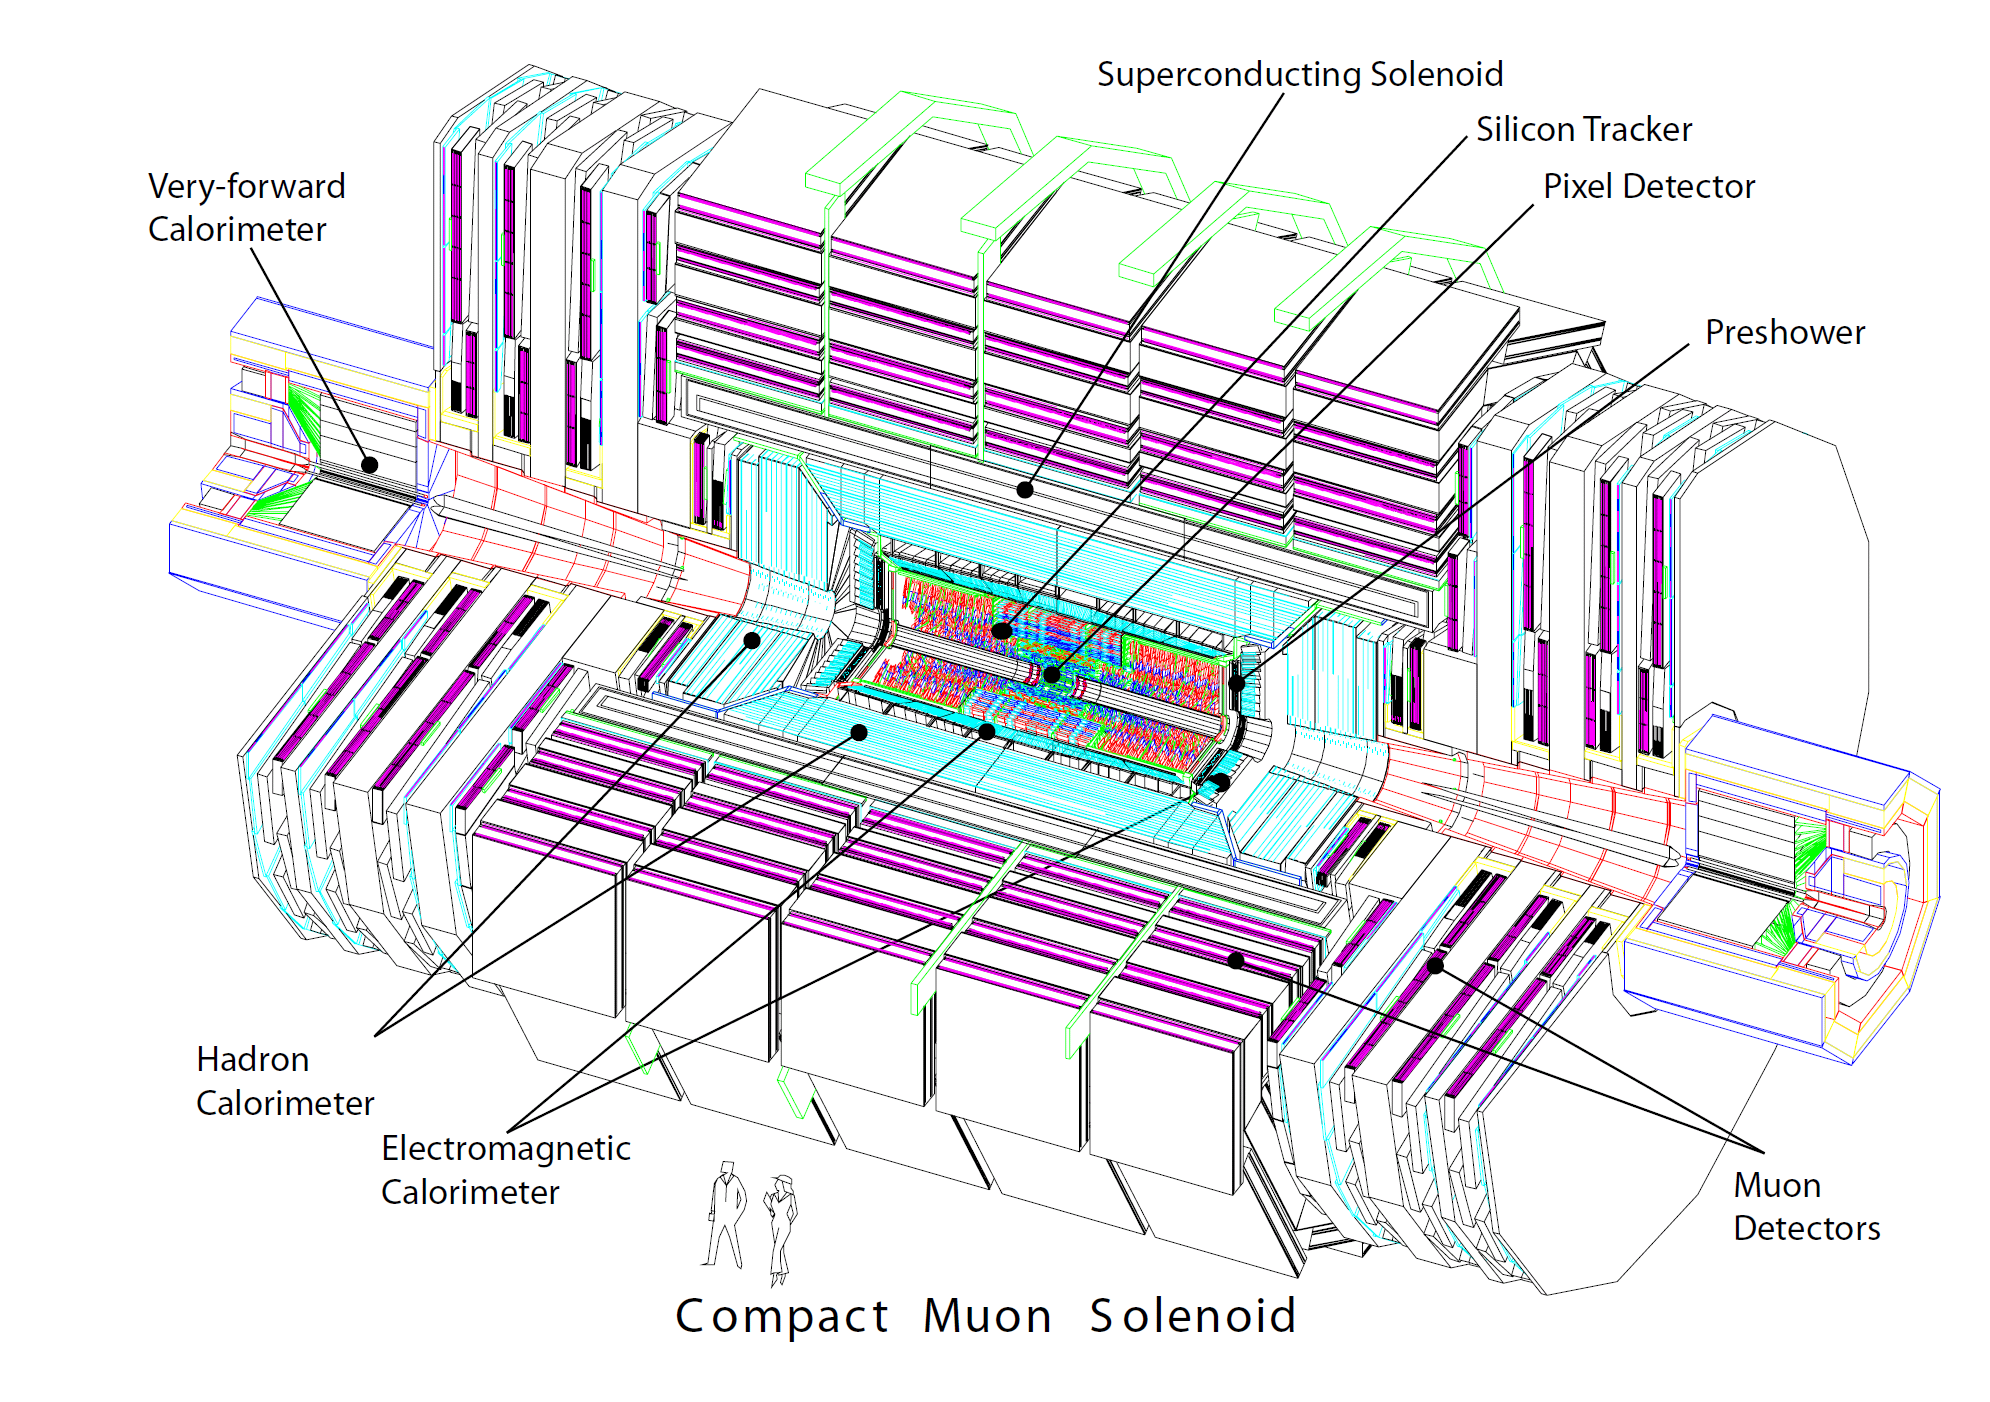
\includegraphics[width=0.75\textwidth]{detector/pics/CMS_apparatus.png}
	\end{tabular}
	\caption{An exploded view of the CMS detector.}
	\label{fig:CMS_apparatus}
\end{figure}

\begin{figure}[tbh!]
	\centering
	\begin{tabular}{cc}
		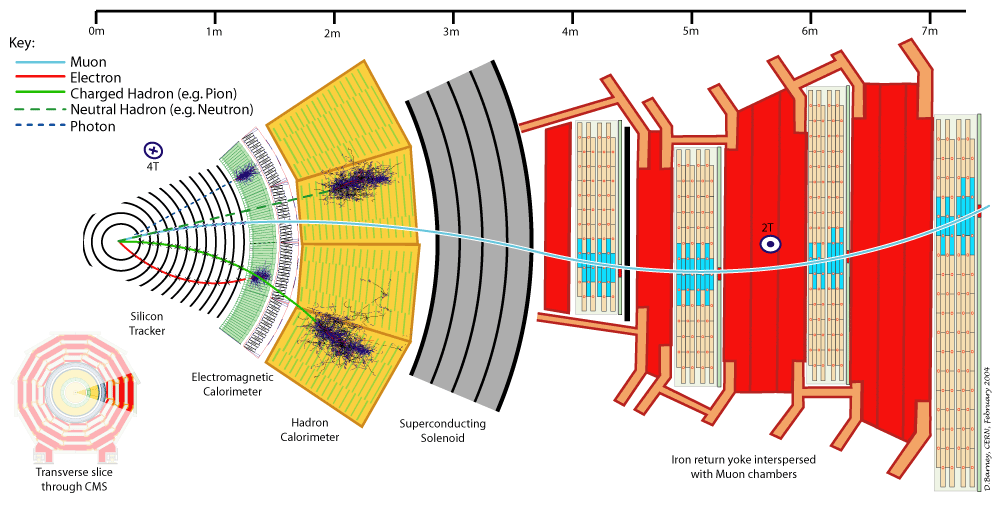
\includegraphics[width=0.75\textwidth]{detector/pics/CMS_slice.png}
	\end{tabular}
	\caption{Longitudinal section of the CMS detector showing the different detectors components and position.}
	\label{fig:CMS_slice}
\end{figure}

\clearpage

\subsection{The Magnet}

The precision requirements of the muon chambers in order to distinguish unambiguously $\approx 1$ TeV/c muon charge is $\Delta p / p \approx 10\%$ therefore the requirement of a magnetic field with high bending power. The main features of the CMS solenoid are the use of a high-purity aluminium-stabilised conductor and indirect cooling (by thermosyphon), together with full epoxy impregnation.

The CMS magnet is large superconducting solenoid with an inner bore of 5.9 m and a length of 12.9 m.  This good length/radius ratio is necessary to ensure good momentum resolution in the forward region as well. Its size is enough to contain the tracking system, the electromagnetic calorimeter and the hadronic calorimeter. 

The high magnetic field of 4 T is generated by a current of 19,5 kA going through 2168 coil turns. An important parameter for this superconducting magnets design is the value of the hoop stress of 64 atm produced by the magnetic pressure due to the Lorentz force. The amount of total energy stored by the superconducting magnet is of 2.7 GJ.

%\begin{figure}[tbh!]
	%\begin{center}
		
	%\begin{tabular}{ | l | l |}
			%\hline
			%Field & 4 T \\ \hline
			%Inner Bore & 5.9 m \\ \hline
			%Length & 12.9 m \\ \hline
			%Number of Turns & 2168  \\ \hline
			%Current & 19.5kA   \\ \hline
			%Stored Energy & 2.7 GJ  \\ \hline
			%Hoop Stress & 64 atm \\
			%\hline
		%\end{tabular}
		%\caption{Parameters of the CMS superconducting solenoid.}
		%\label{table:CMS_magnet}
	%\end{center}
%\end{figure}

\clearpage

\subsection{Inner tracking system}

The Inner Tracking systems reconstructs the track of charged particles and measures their momentum. In order to meet the design requirements of a compact design and high reconstruction efficiency ($95\%$ for high momentum $\mu$ particles) the main detector material is silicon.
The detector can be easily divided in three parts:
\begin{itemize}
	\item Placed close to the interaction point where the particle flux is higher are the pixel detectors. Each pixel is 100×150 $\mu m^{2}$ wide;
	\item In the intermediate region ($20 < r < 55 cm$) the particle flux is low enough to allow the usage of silicon micro-strips, with each cells with the minimum size of $10 cm × 80 \mu m$;
	\item in the outermost region ($r > 55 cm$),the particle flux is low enough to allow bigger size micro-strips with size of $25 cm × 180 \mu m$ 
\end{itemize}

A section of the whole Inner Tracking apparatus on the z-plane is viewable in Figure \ref{fig:Pixel_zview}. Close to the interaction point 3 pixel-layers are placed at radial distances of $4.7$, $7.3$ and $10.2 cm$. In the Barrel region the silicon micro-strips are placed at a radial distance between $20$ and $110 cm$. The forward region has instead 2 pixel and 9 micro-strips layers. The barrel micro-strip section is divided in 2 different parts: the innermost and the outermost one. In order to avoid excessively shallow track crossing angles, the Inner Barrel region is shorter than the Outer one, and there are an additional 3 Inner Disks in the transition region between the Barrel and Endcap parts, on each side of the Inner Barrel. The overall inner layout apparatus is viewable in Figure \ref{fig:Pixel_layout}. The total area of the pixel detector is $\approx 1 m^{2}$, whilst that of the silicon strip detectors is $200 m^{2}$, providing coverage up to $|\eta| < 2.4$. The inner tracker comprises 66 million pixels and $9.6$ million silicon strips. The silicon pixels grants a precision of $10 \mu m$ on the $(x,y)$ transverse plane and of $20 \mu m$ on the z axis. The resolution of the silicon micro-strips depends on each cell thickness, with a minimum value of $ 55 \mu m$ for the traverse plane.


\begin{figure}[tbh!]
	\centering
	\begin{tabular}{cc}
		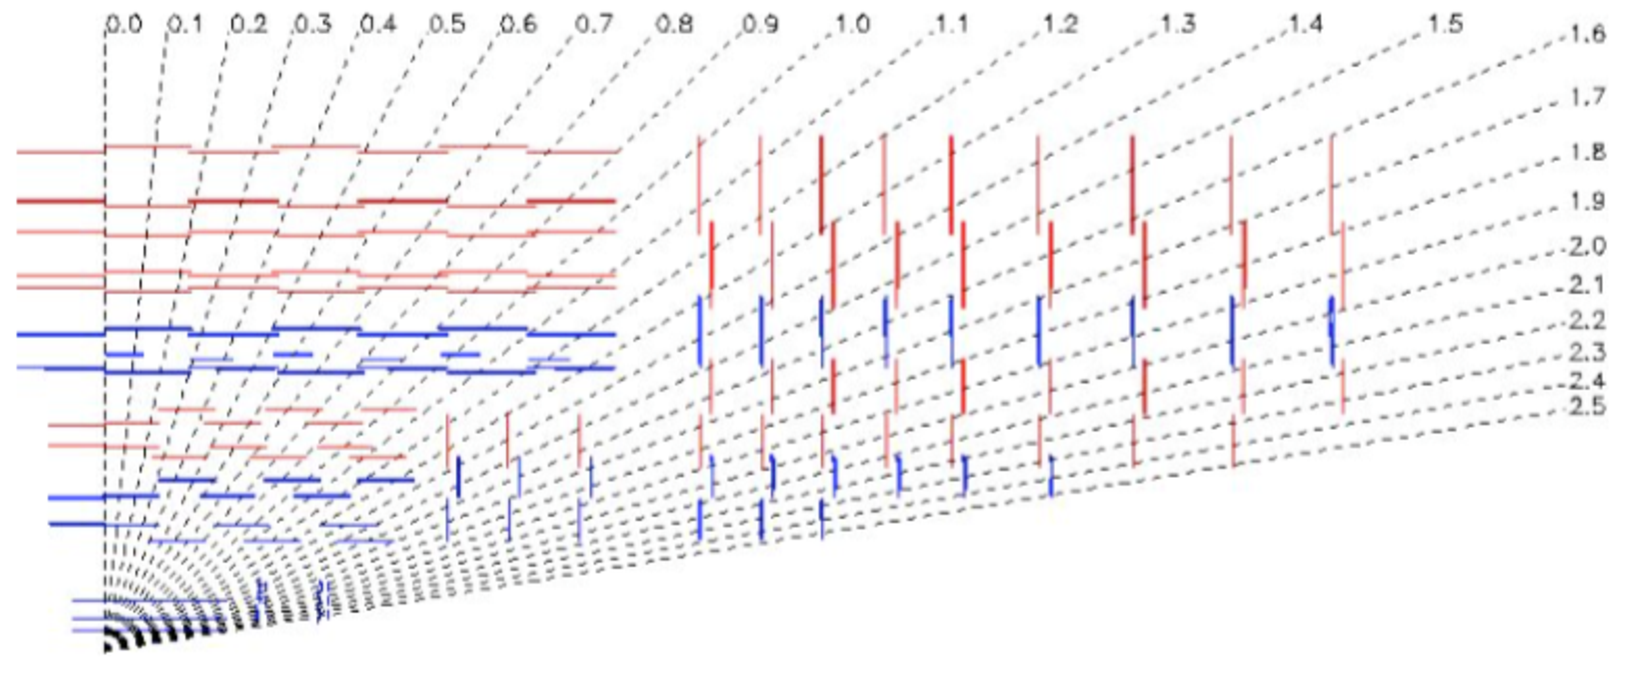
\includegraphics[width=0.75\textwidth]{detector/pics/Pixel_zview.pdf}
	\end{tabular}
	\caption{The tracker layout (1/4 of the z view).}
	\label{fig:Pixel_zview}
\end{figure}

\begin{figure}[tbh!]
	\centering
	\begin{tabular}{cc}
		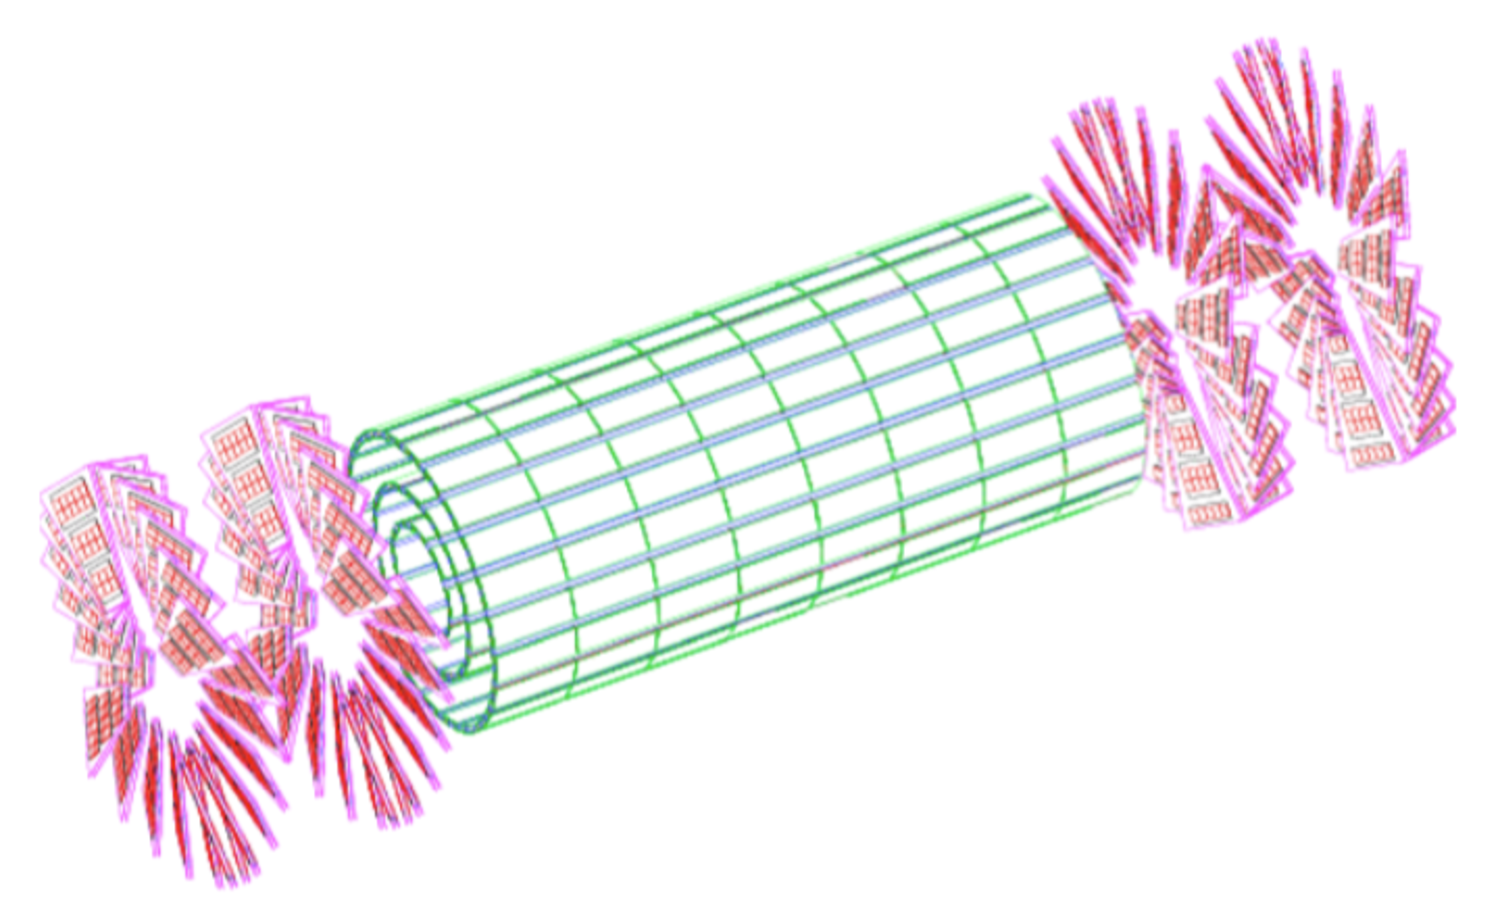
\includegraphics[width=0.75\textwidth]{detector/pics/Pixel_layout.pdf}
	\end{tabular}
	\caption{Layout of pixel detectors in the CMS tracker.}
	\label{fig:Pixel_layout}
\end{figure}

\clearpage

\subsection{The Electromagnetic calorimeter}

The Electromagnetic Calorimeter (ECAL) is a hermetic, homogeneous calorimeter comprising 61200 lead tungstate ($PbWO_{4}$) crystals mounted in the central barrel part, closed by 7324 crystals in each of the 2 endcaps.
The the crystal material choice was driven by the short radiation length and Molière ray, granting compactness and good granularity as listed on Table \ref{table:CMS_PbWO4}. Other $PbWO_{4}$ important properties are radiation resistance and the short decaying time witch allows to collect the $85\%$ of light during the $25$ ns interval between a bunch crossing and the next one.

\begin{figure}[tbh!]
	\begin{center}
		
		\begin{tabular}{ | l | c |}
			\hline
			Density  & $ 8.28 g/cm^{3}$ \\ \hline
			$X_{0}$   & $0.89 cm$  \\ \hline
			$R_{M}$ 2.2 & $2.2 cm$  \\ \hline
			\hline
		\end{tabular}
		\caption{Parameters of the $PbWO_{4}$ crystals .}
		\label{table:CMS_PbWO4}
	\end{center}
\end{figure}

The Ecal is made of a central body in the Barrel region and two identical structures covering the Endcap ones. The final design aim was to build a calorimeter as compact as possible. In order to have high hermeticity the space in between crystals has been reduced as much as possible especially in the transition region between Barrel and Endcaps. 

The Barrel covers a pseudo-rapidity region of $|\eta| < 1.479$ with its cylinder ray of 129 cm. It contains 61200 crystals; 360 placed in $\phi$ and $2\times85$ in $\eta$. The crystals are quasi-projective (the axes are tilted at $3^{\circ}$ with respect to the line from the nominal vertex position) and cover $0.0174$ (i.e. $1^{\circ}$) in $\Delta\phi$ and $\Delta\eta$. The crystals have a front face cross-section of $\approx 22\times22 mm^{2}$ and a length of 230 mm, corresponding to $25.8 X_{0}$. The Endcaps cover the pseudo-rapidity of $1.48 < |\eta| < 2.6$ where the $2.6\times2.6\times22 cm^{3}$ are gathered in $5\times5$ matrices called supercrystals.

In the pseudo-rapidity interval of $1.653 < |\eta| < 2.56$, as shown on Figure \ref{fig:ECAL_section}, is present a detector called Preshower, halo-ring shaped. The preshower is a sampling calorimeter made by two distinct layers; the showering layer made of lead and the detector layer made of silicon strips capable of measuring the energy deposit of the initial part of particle showers as well as their lateral profile. The role of this detector is important whenever multiple particle showers overlap in the ECAL Endcap allowing a clear distinction of each of those showers.

The overall ECAL resolution can be parametrized as a function of the energy measured:

\begin{equation}
\dfrac{\sigma}{E}^{2} = \dfrac{S}{\sqrt{E}}^{2} + \dfrac{N}{E}^{2} + C^{2}
\end{equation}

where S is the stochastic term, N the noise and C the constant term. The values of these
parameters are listed on Figure \ref{fig:ECAL_resolution}.  

\begin{figure}[tbh!]
	\centering
	\begin{tabular}{cc}
		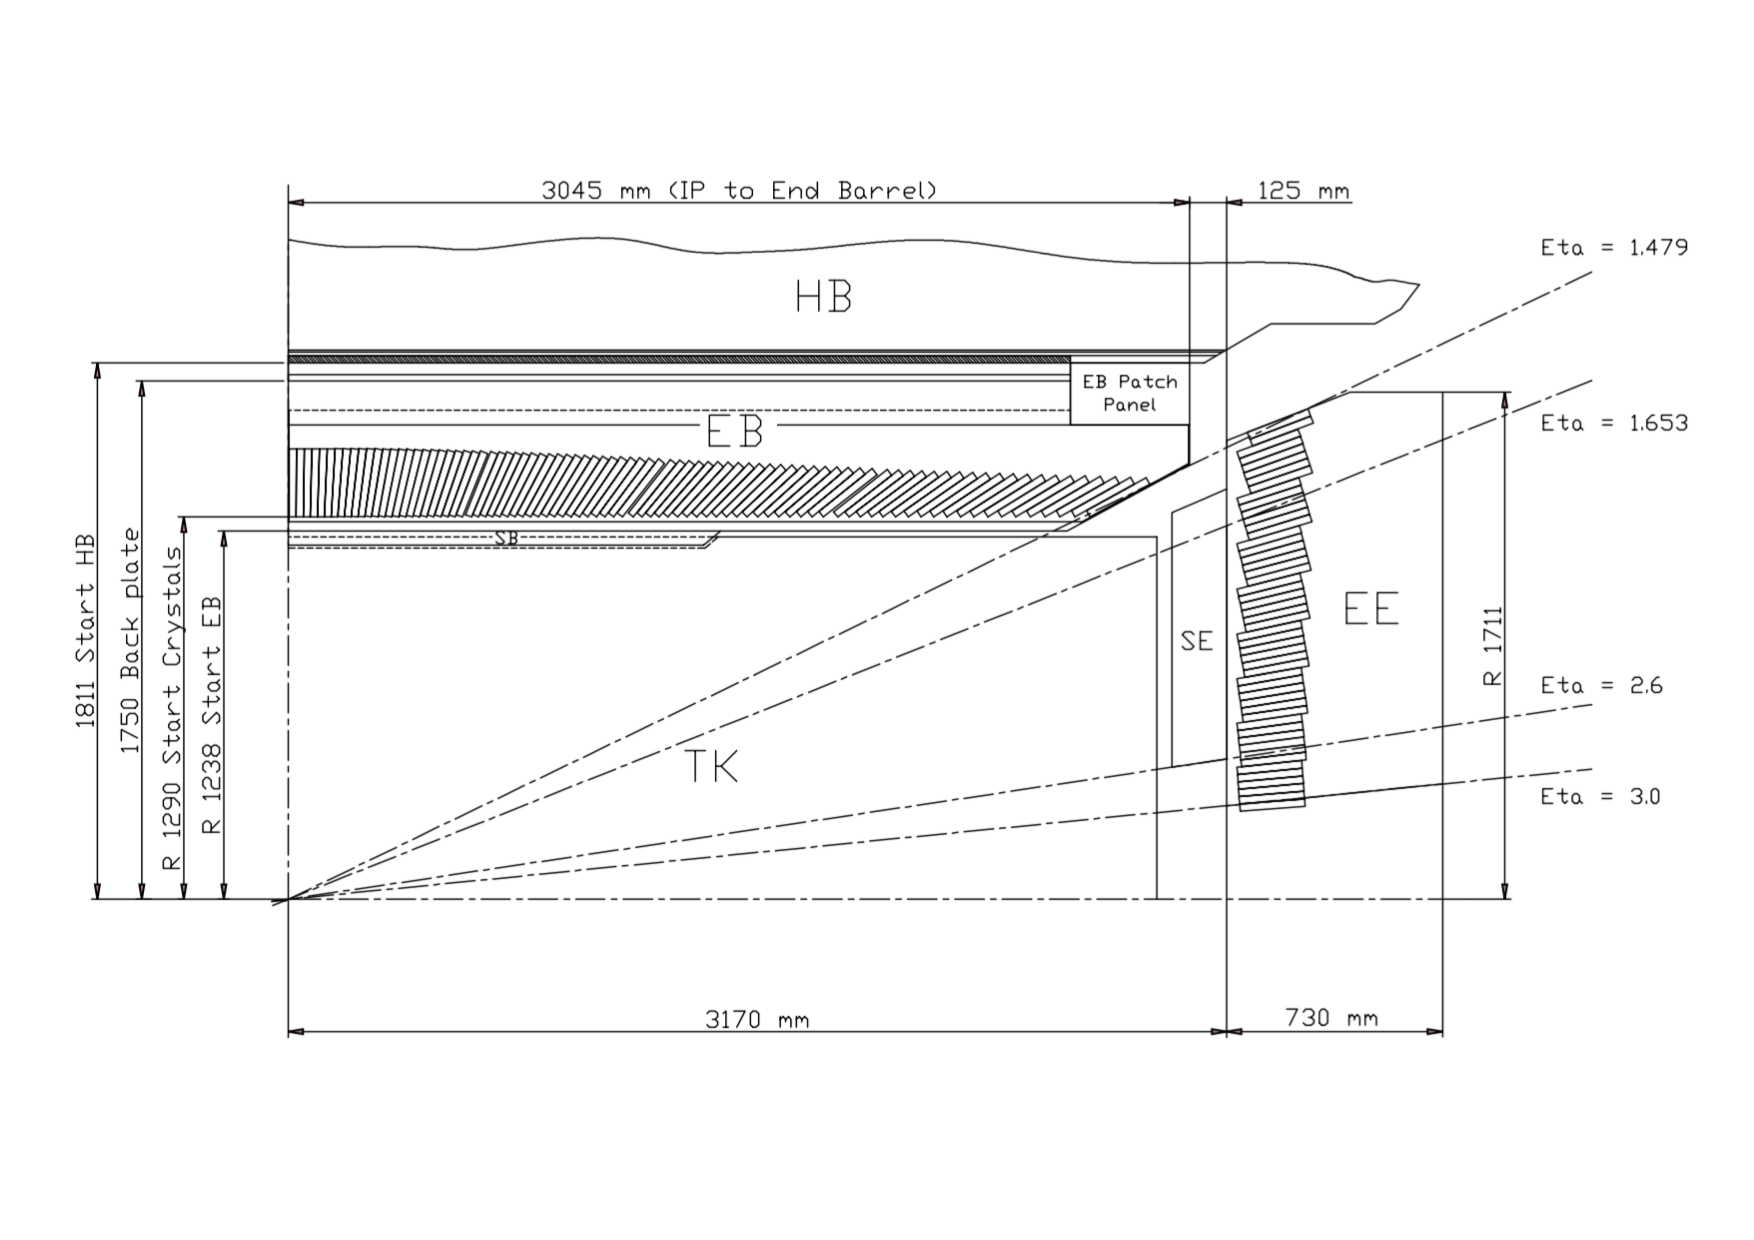
\includegraphics[width=0.75\textwidth]{detector/pics/ECAL_section.pdf}
	\end{tabular}
	\caption{Longitudinal section of the electromagnetic calorimeter (one quadrant).}
	\label{fig:ECAL_section}
\end{figure}

\begin{figure}[tbh!]
	\centering
	\begin{tabular}{cc}
		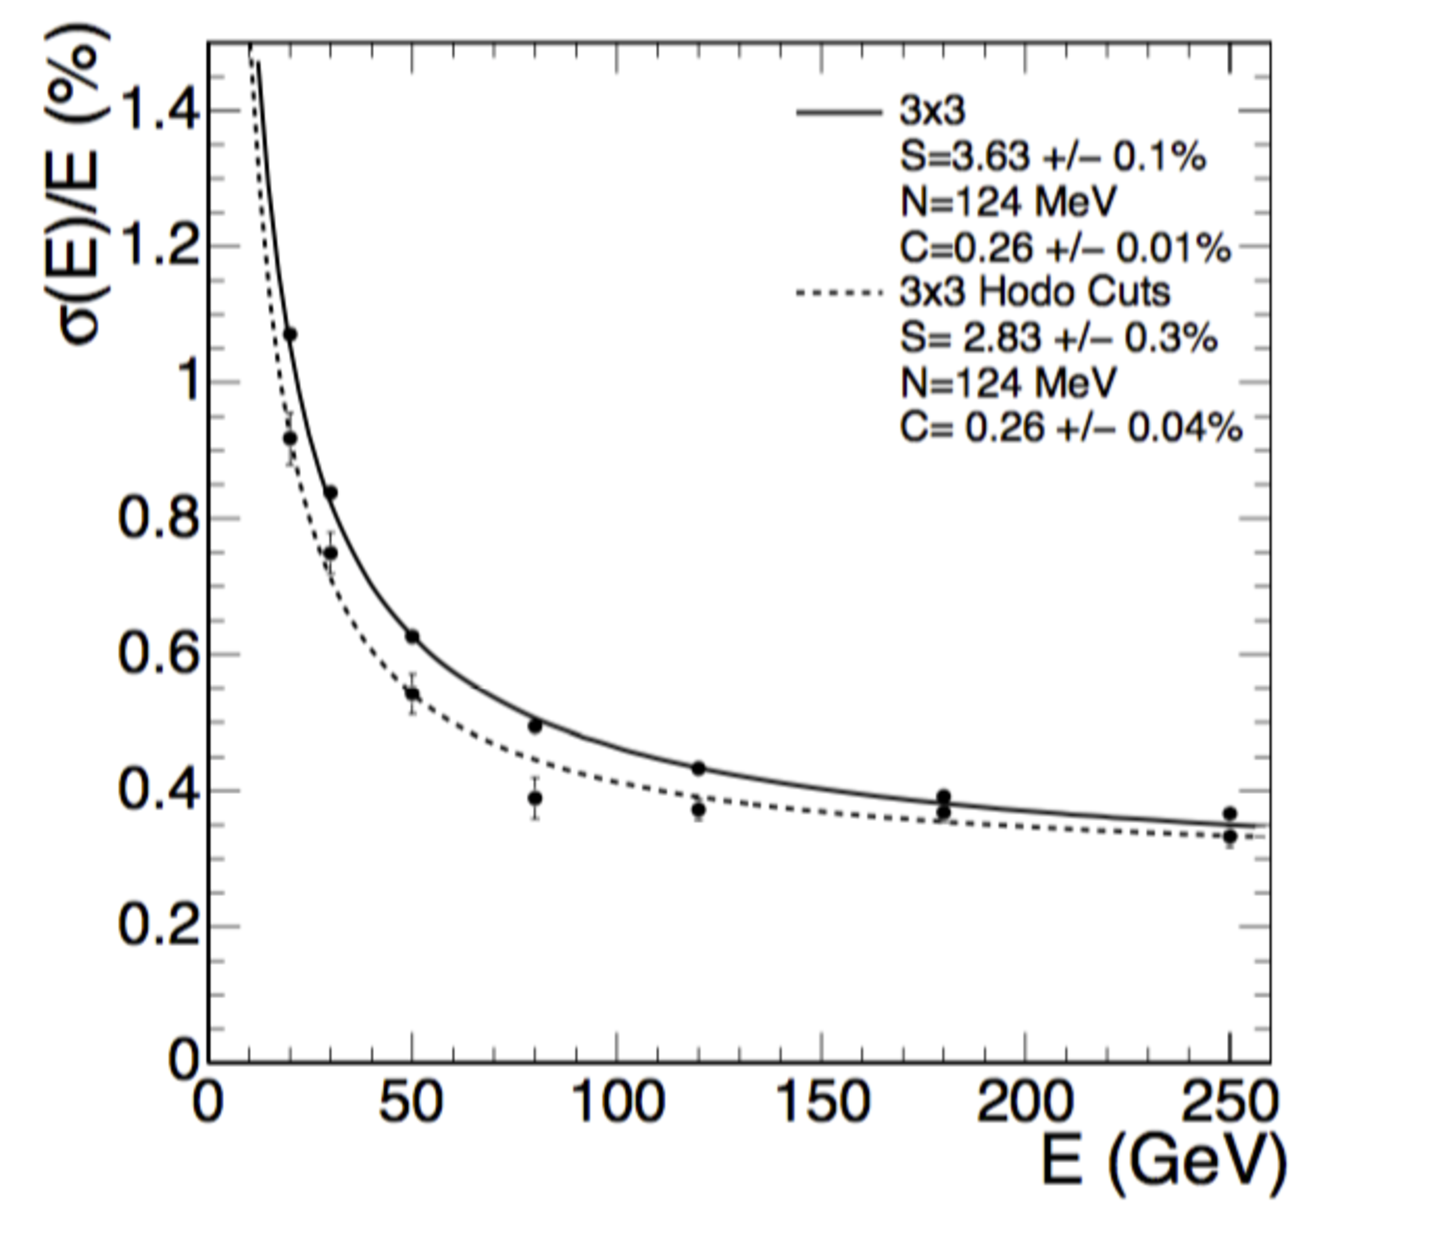
\includegraphics[width=0.75\textwidth]{detector/pics/ECAL_resolution.pdf}
	\end{tabular}
	\caption{ECAL supermodule energy resolution, $\sigma_{E}/E$, as a function of electron energy as measured from a beam test. The upper series of points correspond to events taken with a $20x20 mm^{2}$ trigger and. The lower series of points correspond to events selected to fall within a $4x4 mm^{2}$ region. The energy was measured in an array of $3x3$ crystals with electrons impacting the central crystal.}
	\label{fig:ECAL_resolution}
\end{figure}

\clearpage

\subsection{The Hadron calorimeter}

The Hadronic Calorimeter (HCAL) is used along side with the electromagnetic one in order to measure the energy deposit and position in the detector for hadronic jets, the transverse energy and the missing transverse energy $\met$. The requirements for this detector are to minimize as much as possible the Gaussian tail of the resolution distribution and good containment of the hadronic showers in order to have good $\met$ measurements. Its design is influenced by the choice of the magnet parameters since is located inside the superconducting magnet along with the ECAL and the inner tracking system. 

The hadron Barrel (HB) part of HCAL consists of 32 towers covering the pseudo-rapidity region $−1.4 < \eta < 1.4$, resulting in 2304 towers with a segmentation $\Delta\eta\times\Delta\phi = 0.087\times0.087$, corresponding to a $5x5$ ECAL crystal tower. The HB is constructed in 2 half barrels. The HB is readout as a single longitudinal sampling. There are 15 brass plates, each with a thickness of about 5 cm, plus 2 external stainless steel plates for mechanical strength. Particles leaving the ECAL volume first see a scintillator plate with a thickness of 9 mm rather than 3.7 mm for the other plates. The light collected by the first layer is optimized to be a factor of about 1.5 higher than the other scintillator plates. The radiation length $\lambda_{0}$ for HB is $8.9$.

Each hadron Endcap (HE) of HCAL consists of 14 $\eta$ towers with $5^{\circ}$ $\phi$ segmentation,covering the pseudo-rapidity region $1.3 < |\eta| < 3.0$. For the 5 outermost towers (at smaller $\eta$) the $\phi$ segmentation is $5^{\circ}$ and the $\eta$ segmentation is 0.087. For the 8 innermost towers the $\phi$ segmentation is $10^{\circ}$, whilst the $\eta$ segmentation varies from 0.09 to 0.35 at the highest $\eta$. The total number of HE towers is 2304. The radiation length $\lambda_{0}$ for HE is $10.0$.

In order to improve the shower containment there's another calorimeter, called "Tail catcher" placed right outside the magnet. As further hermeticity improvement a "forward" calorimeter (HF) has been installed at around $11$ meters from the interaction point, covering the $\eta$ region of $3.0 < |\eta| <5.0$. This calorimeter is made of steel/quartz fibres running paralel to the beam line.

Figure \ref{fig:HCAL_section} shows the longitudinal section of the HCAL and the locations of its parts HB, HE, HF and HO.

The HCAL energy resolution is:

\begin{equation}
\dfrac{\sigma(E)}{E} = \dfrac{100\%}{\sqrt{E}}\oplus 4.5\%
\end{equation}

\begin{figure}[tbh!]
	\centering
	\begin{tabular}{cc}
		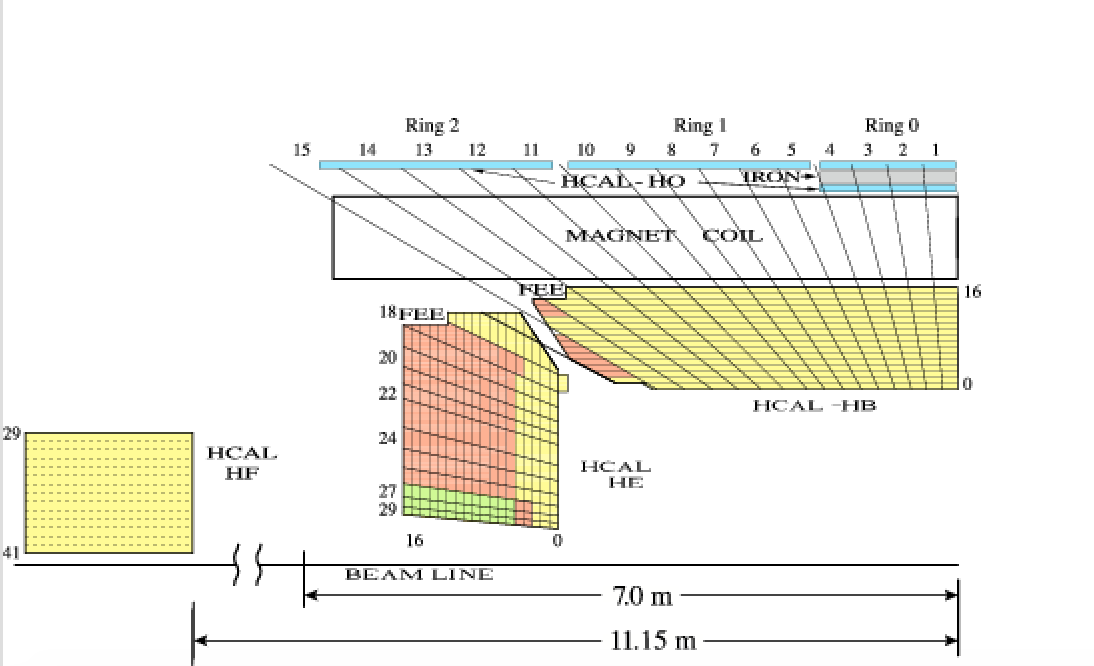
\includegraphics[width=0.75\textwidth]{detector/pics/HCAL_section.png}
	\end{tabular}
	\caption{The CMS HCAL detector (quarter slice). "FEE" indicates the locations of the Front End Electronics for HB and HE. The signals of the tower segments with the same color are added optically, to provide the HCAL "longitudinal" segmentation. HB, HE and HF are built of 36 identical azimuthal wedges\,($\Delta\phi = 20$ degrees).}
	\label{fig:HCAL_section}
\end{figure}

Table \ref{fig:HCAL_resolution} shows the distribution of the jet energy resolution as function of the simulate jet traverse energy.

\begin{figure}[tbh!]
	\centering
	\begin{tabular}{cc}
		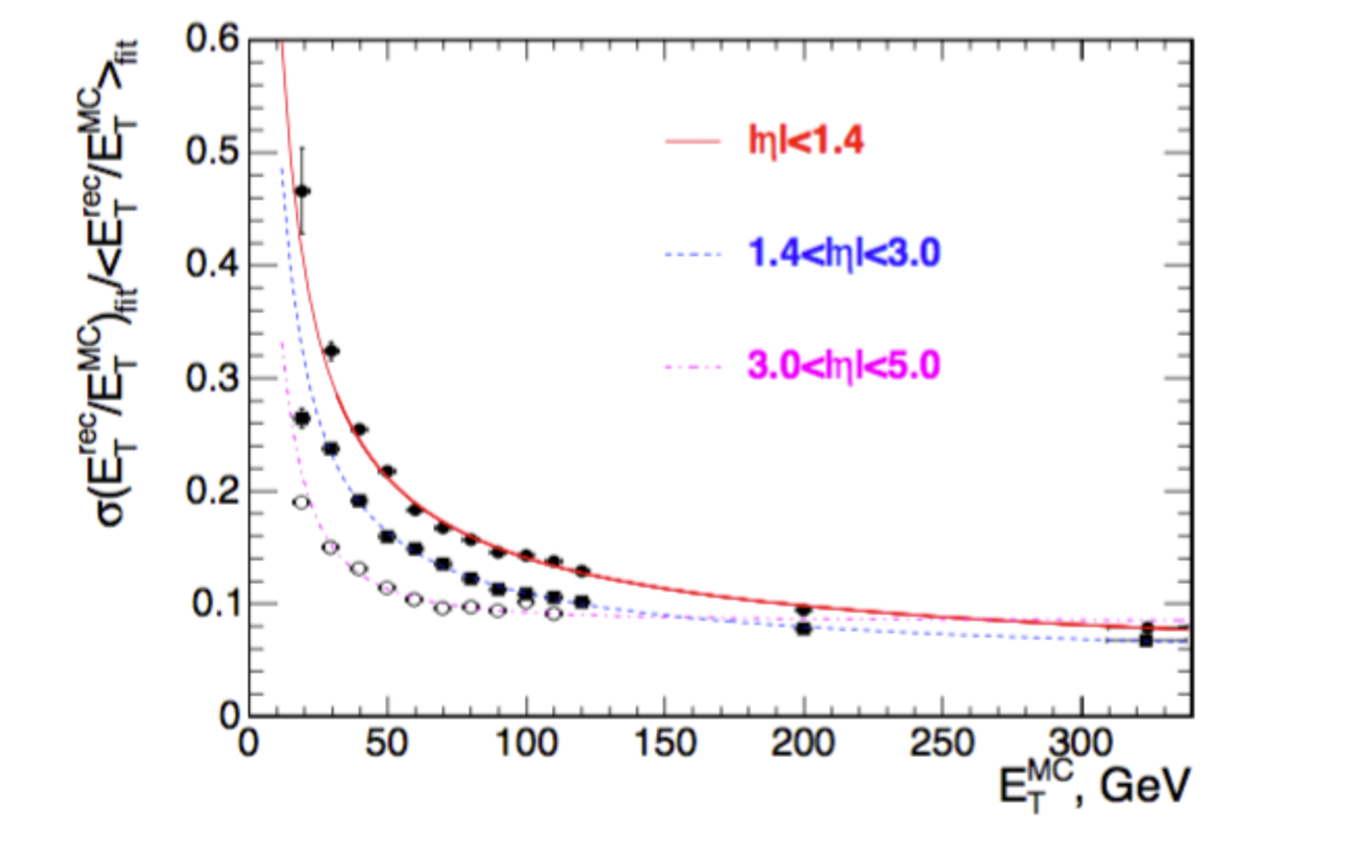
\includegraphics[width=0.75\textwidth]{detector/pics/HCAL_resolution.pdf}
	\end{tabular}
	\caption{The jet transverse energy resolution as a function of the simulated jet transverse energy for barrel jets $(|\eta| < 1.4)$, endcap jets $(1.4 < |\eta| < 3.0)$ and very forward jets $(3.0 < | \eta | < 5.0)$. The jets are reconstructed with the interative cone $R = 0.5$ algorithm.}
	\label{fig:HCAL_resolution}
\end{figure}

\clearpage

\subsection{The Muon System}

\begin{figure}[tbh!]
	\centering
	\begin{tabular}{cc}
		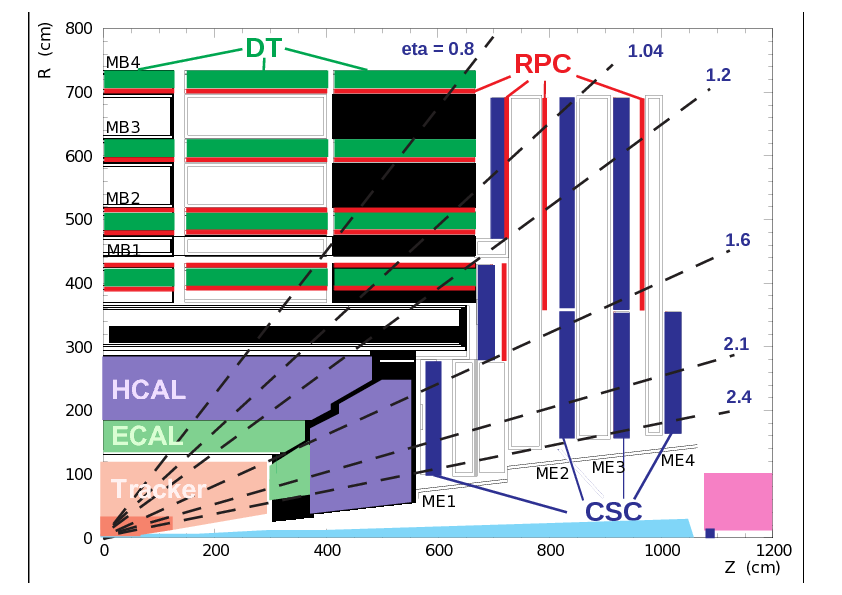
\includegraphics[width=0.75\textwidth]{detector/pics/CMS_muonsys.png}
	\end{tabular}
	\caption{Layout of one quarter of the CMS muon system for initial low luminosity running.
		The RPC system is limited to $|\eta| < 1.6$ in the endcap, and for the CSC system only the inner
		ring of the ME4 chambers have been deployed.}
	\label{fig:CMS_muonsys}
\end{figure}

Three types of gaseous detectors are used to identify and measure muons \ref{muondetectors}. The choice of the detector technologies has been driven by teo reasons: the high radiation environment and the large surface to cover. Since in the barrel region of $|\eta| < 1.2$, both the muon rate and the residual magnetic field in the chambers is low, drift tube (DT) chambers are used. In the 2 endcaps insted, where the muon rate as well as the neutron induced background rate is high, and the magnetic field is also high, cathode strip chambers (CSC) are placed covering the pseudo-rapidity region up to $|\eta| < 2.4$. Additionally, resistive plate chambers (RPC) are used in both the barrel and the endcap regions covering a pseudo-rapidity region of $|\eta| < 2.1$. These RPCs operate in avalanche mode to ensure good performances at high rates and have double gaps with a gas gap of 2 mm. RPCs provide a fast response with good time resolution but with a coarser position resolution than the DTs or CSCs. RPCs can therefore identify unambiguously the correct bunch crossing.

The DTs or CSCs and the RPCs operate within the first level trigger system, providing independent and complementary sources of information.
The layout of one quarter of the CMS muon system for initial low luminosity running is shown in Figure \ref{fig:CMS_muonsys}. In total, the muon system contains of order 25000 $m^{2}$ of active detection planes, and nearly 1 million electronic channels.

\clearpage

\subsection{The Trigger System}

With a bunch crossing rate of 40 Mhz at design luminosity and the possibility to record the information for $\approx 10^{2}$ crossings/sec the CMS experiment needs a trigger system capable of a rejeftion factor of at least $10^{6}$.

The CMS trigger and data acquisition system (DAQ) consist of 4 parts: the detector electronics, the hardware-based level 1 trigger, the readout network and and the online event filter system that uses a software-based high level trigger (HLT).

There's a minimum transit time required for the signal to reach the level one trigger hardware based on the service tunnels next to the CMS experiment site, wait for the trigger response to keep or discard the event and send it back to the detectors readout apparatus. The average time needed for a single cycle is 3.2 $\mu s$. During the following time the event information is stored in a buffer waiting for the Level-1 trigger response. The trigger decisional time is less than 1 $\mu s$ with a rejection power of around 1 crossing kept every 1000.

The Level-1 decision is based on "trigger primitive" objects such as photons, electrons and muons and jets above thresholds as well as the transverse energy $E_{T}$ and the missing transverse energy \met involving the calorimetry and the muon system and a combination between these detectors. Since the Level-1 trigger is meant to take fast decisions at a high rate (the design value is 100kHz) the trigger objects are reconstructed with reduced resolution and granularity. A safe time margin of a factor of 3 is taken into account in order to cover for possible reconstruction uncertainties as well as beam and detector conditions leading to a rate of 16kHz. The design value of 100 kHz is set by the average time to transfer full detector information through the readout system. A schematic overview of the Level-1 Trigger structure is shown on figure \ref{fig:trigger_lvl1}.

Once an event passes the Level-1 trigger selection the data from the pipelines to the front end readout buffers waiting for a further event reconstruction. After a successful reconstruction the compressed event is sent to one processors of the available farm that runs the same High Level Trigger (HLT) software. The main aim of the HLT is to gather all the informations collected in the event in order to trigger over more complex objects such as $\tau$ particles, multiple jets and multiple particle object or event reconstructed quantities in order to further reduce the event rate from 100kHz to 100Hz for mass storage.

\clearpage

\subsection{Software and Computing}

The CMS software and computing systems covers a broad range of tasks:

\begin{itemize}
	\item online and offline calibration and status reports for each of the subdetectors;
	\item management, maintenance and access of the data storage;
	\item reconstruction and analysis of data;
	\item support of the distributed computing infrastructure and software framework.
\end{itemize}

The scale of the CMS collaboration in terms of storage capabilities, networking power is orders of magnitude higher that the CERN's infrastructure capabilities. Therefore the CMS computing model is highly distributed, with a primary "Tier-0" centered at CERN with the additional support by "Tier-1" and "Tier-2" computing centers scattered worldwide in several universities and research centers. 

\begin{figure}[tbh!]
	\centering
	\begin{tabular}{cc}
		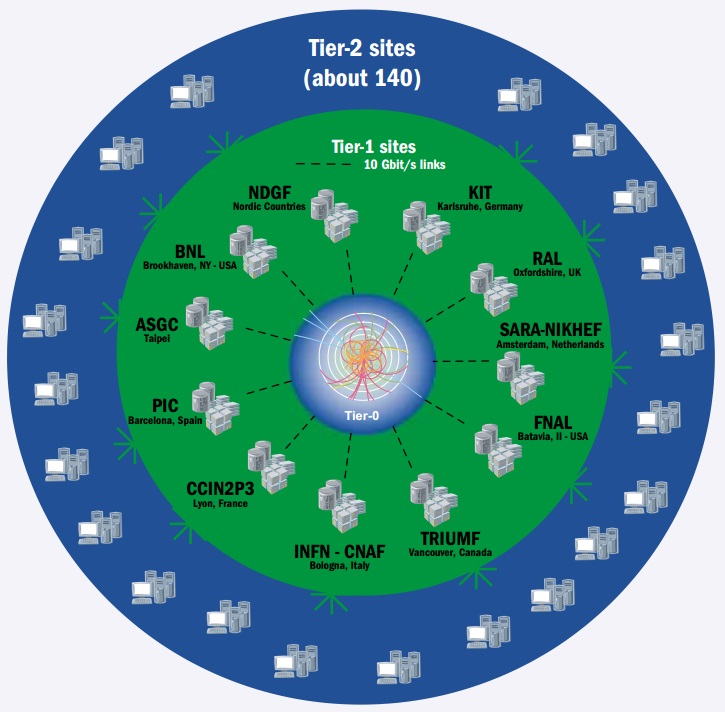
\includegraphics[width=0.75\textwidth]{detector/pics/CMS_grid.jpg}
	\end{tabular}
	\caption{Overview of the structure of the CMS Computing Grid.}
	\label{fig:CMS_grid}
\end{figure}

The scale of the CMS collaboration in terms of storage capabilities, networking power is orders of magnitude higher that the CERN's infrastructure capabilities. Therefore the CMS computing model is highly distributed consisting of four layers, or "tiers"; 0, 1, 2 and 3. Each tier provides a specific set of services.

All those facilities as shown on Figure \ref{fig:CMS_grid} have hierarchical structure under the Tier-0 and go under the name of "CMS Computing Grid".

\subsubsection{Tier-0}

This is the CERN Data Centre, which is located in Geneva, Switzerland and also at the Wigner Research Centre for Physics in Budapest, Hungary over 1200km away. The two sites are connected by two dedicated 100 Gbit/s data links. All data from the LHC passes through the central CERN hub, but CERN provides less than $20\%$ of the total compute capacity.

Tier 0 is responsible for the safe-keeping of the raw data (first copy), first pass reconstruction, distribution of raw data and reconstruction output to the Tier 1s, and reprocessing of data during LHC down-times.

\subsubsection{Tier 1}

These are thirteen large computer centres with sufficient storage capacity and with round-the-clock support for the Grid. They are responsible for the safe-keeping of a proportional share of raw and reconstructed data, large-scale reprocessing and safe-keeping of corresponding output, distribution of data to Tier 2s and safe-keeping of a share of simulated data produced at these Tier 2s.

\subsubsection{Tier 2}

The Tier 2s are typically universities and other scientific institutes, which can store sufficient data and provide adequate computing power for specific analysis tasks. They handle analysis requirements and proportional share of simulated event production and reconstruction.

There are currently around 160 Tier 2 sites covering most of the globe.

\subsubsection{Tier 3}

Individual scientists will access these facilities through local (also sometimes referred to as Tier 3) computing resources, which can consist of local clusters in a University Department or even just an individual PC. There is no formal engagement between WLCG and Tier 3 resources. 


\cleardoublepage

\chapter{Search for SUSY in Vector Boson Fusion Processes at the LHC}
\label{sec:VBFSUSY}
\section {Introduction}

Many of the searches for \charginopm and \neutralinotwo in ATLAS \cite{Aad:2012hba, ATLAS:2012ab} and CMS \cite{Chatrchyan:2012mea} involves the search for signal events with 3 leptons and \met. On the other hand there are very few searches involving final states with $\tau$ leptons due to the the larger $\tau$ misidentification rate which makes harder to keep the background under control as well as having low \pt thresholds for triggering.

There is however the possibility to study final states with $2\tau$ and \met coming from the decay of \charginopm and \neutralinotwo produced by Vector Boson Fusion (VBF) processes. This search comes with some important advantages.

Firstly with the increasing LHC luminosity both ATLAS and CMS needs to raise the \pt thresholds on the triggered objects. Is it possible however to probe signal for SUSY in VBF events by triggering over the VBF properties of the event, leaving the decay products of \charginopm and \neutralinotwo free from trigger bias. 

Secondly scenarios involving the naturalness of SUSY allows \stau lighter than \smuon and \selectron for high values of \tanbeta. A light \stau with small mass splitting also is favored in coannihilation processes \cite{Griest:1990kh} that set the relic density to correct values, in the case of Bino dark matter. Light \stau is also motivated in the context of the MSSM by the enhancement of the $H \longrightarrow \gamma\gamma$ channel \cite{Carena:2011aa}. All of these facts stress on the importance of the search for low \pt $\tau$ final states with large background contribution, for which production by the VBF processes since is possible to take advantage of its signature in order to reduce the background contribution. 

As third and final reason a VBF based searches are complementary to the existing one at LHC based on Drell-Yan production since is not constrained by any trigger bias. 

\begin{figure}[tbh!]
	\centering
	\begin{tabular}{cc}
		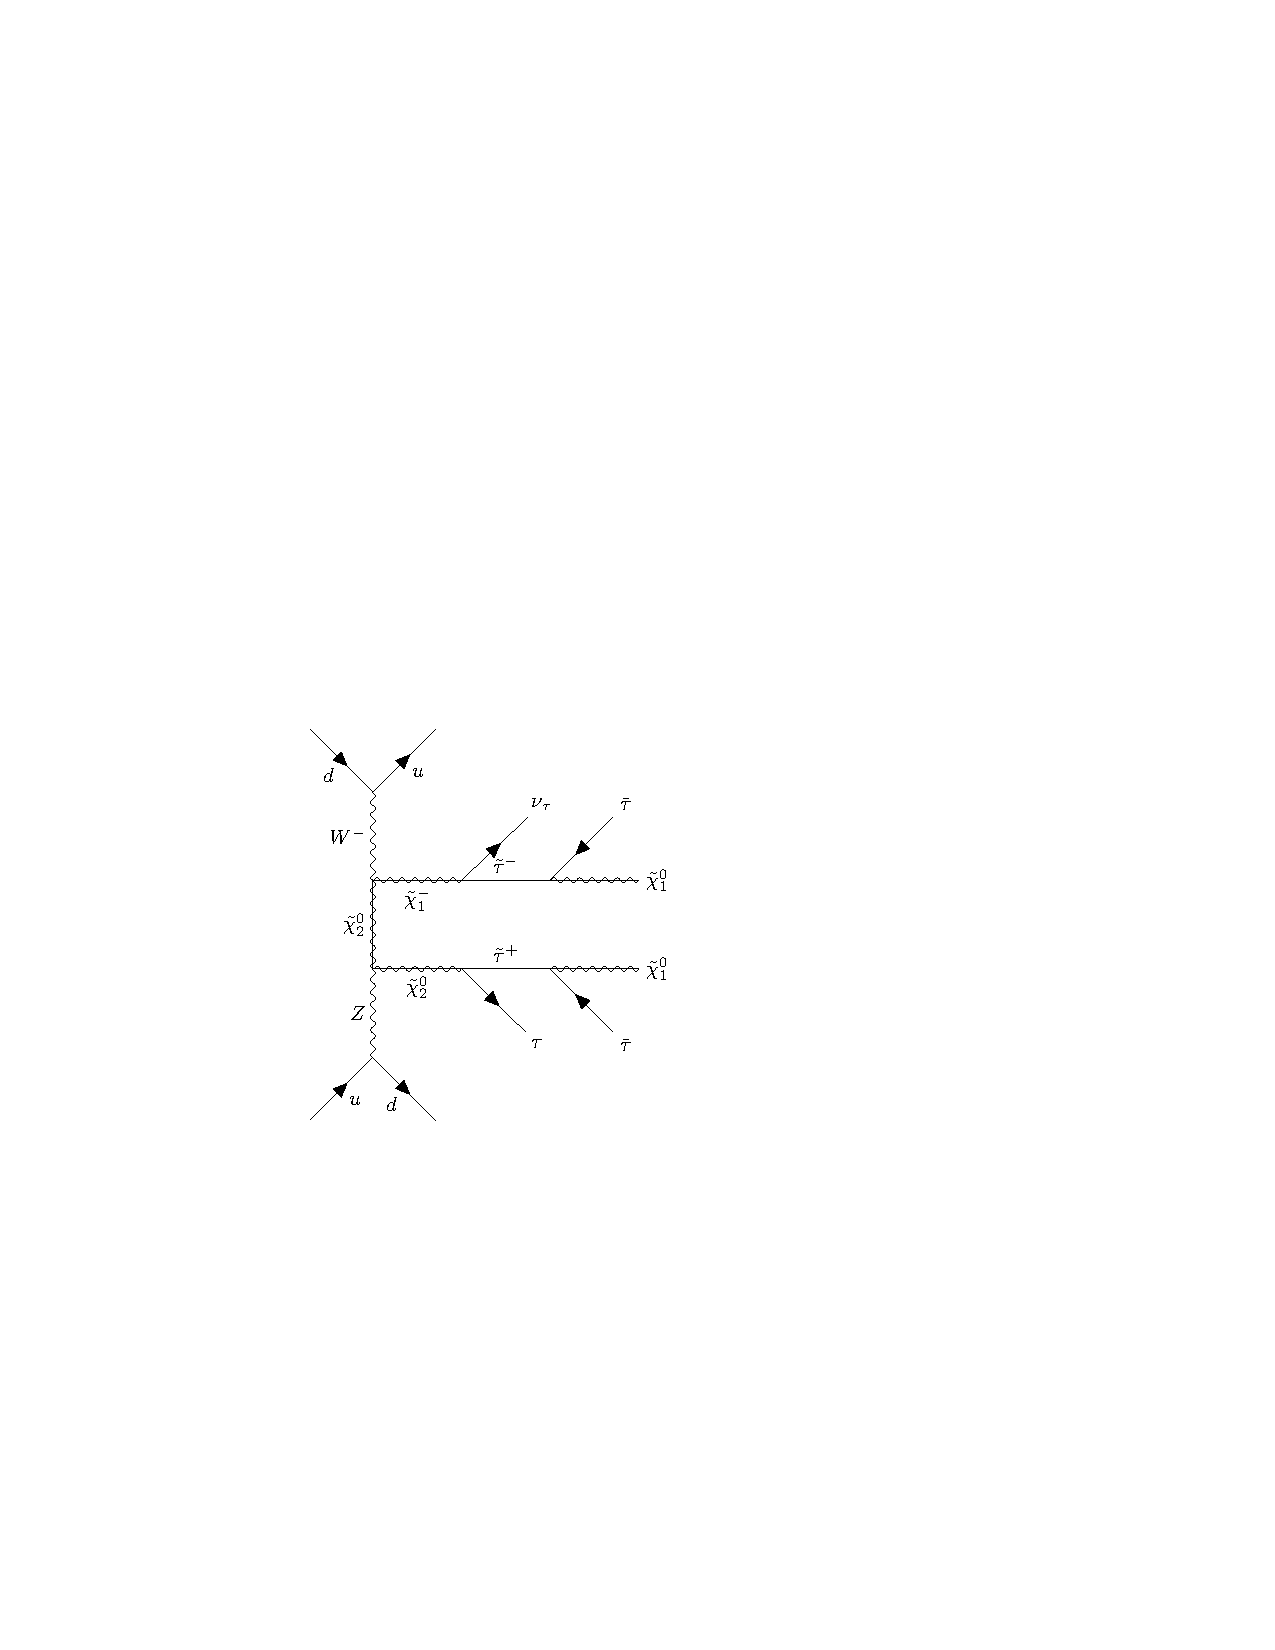
\includegraphics[width=0.50\textwidth]{diagrams/pics/signal_C1N2.pdf}
		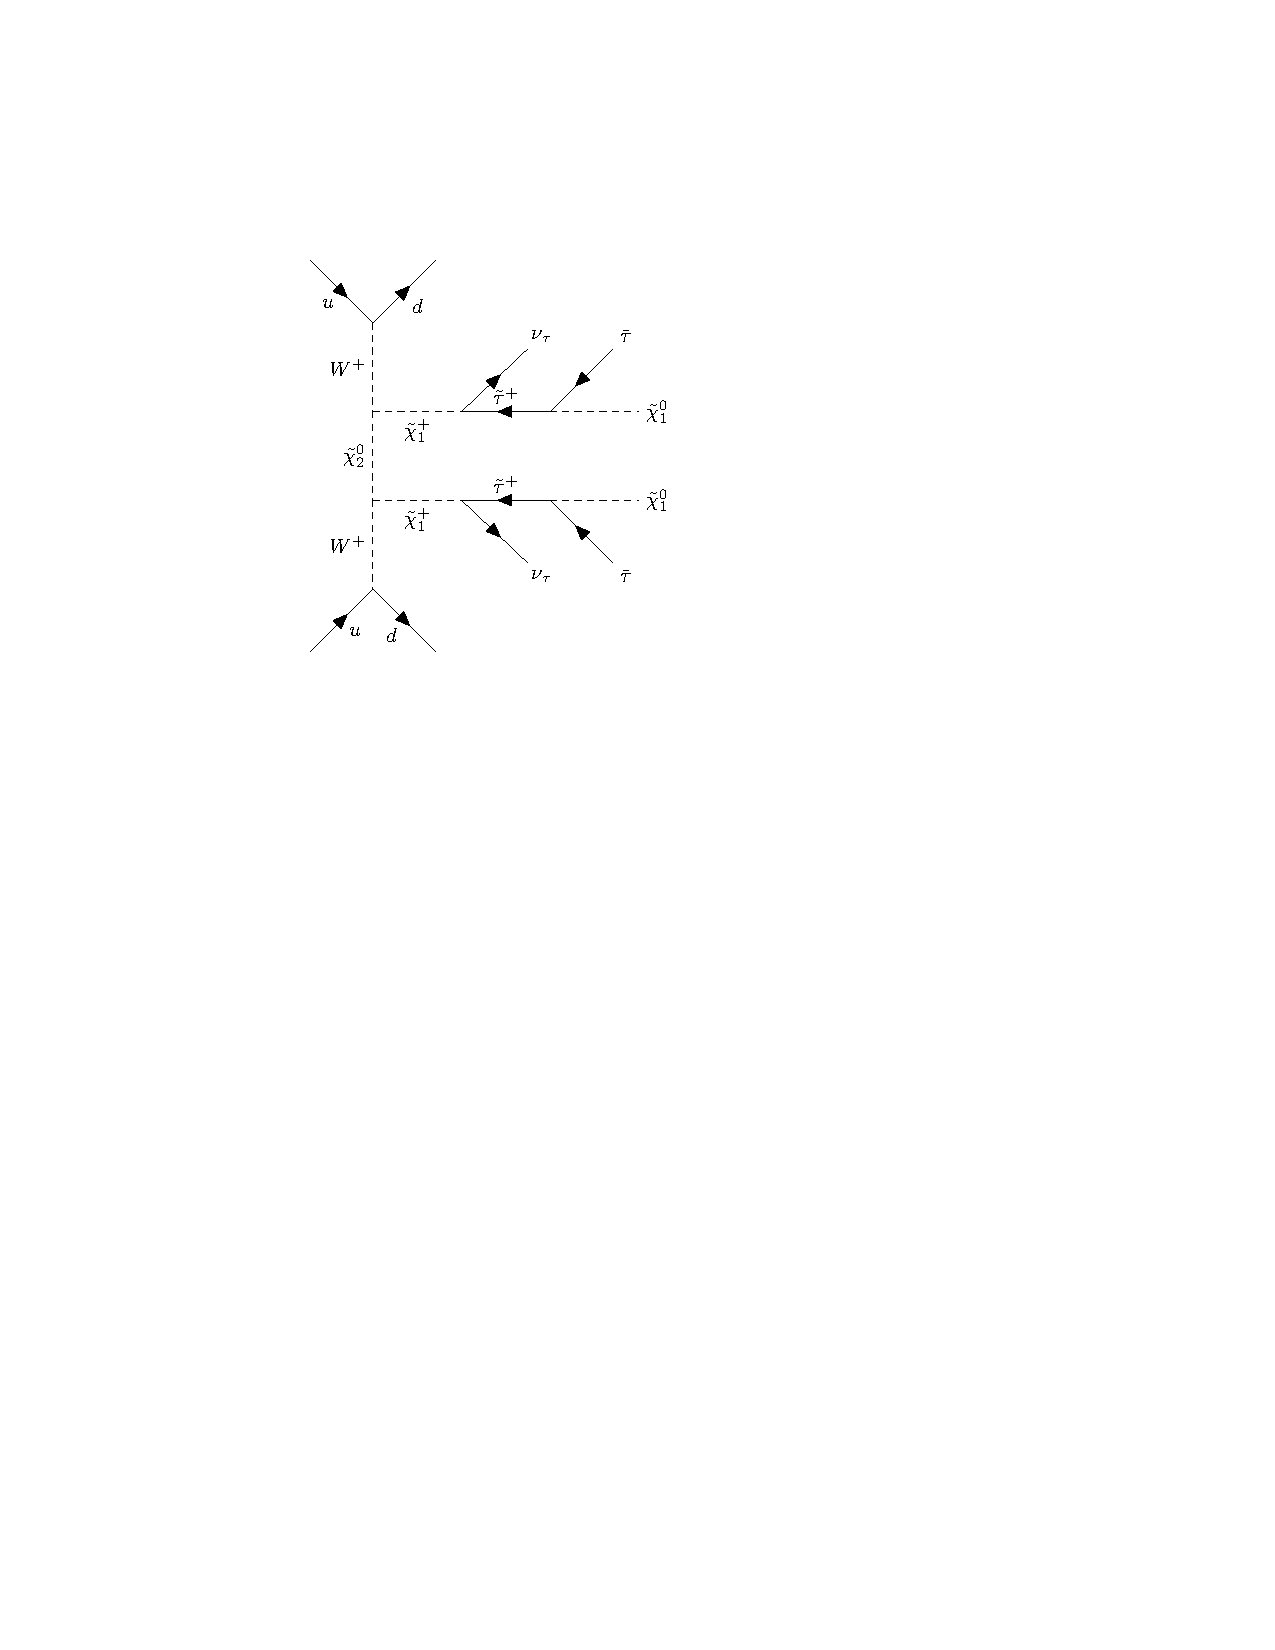
\includegraphics[width=0.50\textwidth]{diagrams/pics/signal_C1C1.pdf} 		
	\end{tabular}
	\caption{Diagrams of (left) \charginopm \neutralinotwo and (right) \charginopm \charginomp pair production through vector-boson fusion followed by their decays to $\tau$ leptons and the LSP.}
	\label{fig:VBF_diagrams}
\end{figure}

The Feynman diagrams for the typical \charginopm \neutralinotwo pair production are shown on  Figure \ref{fig:VBF_diagrams}. The \charginopm and \neutralinotwo coming from the VBF processes decays into the multiple leptons and \neutralinoone final state with the following decay process for \charginopm

\begin{equation}
\charginopm \longrightarrow \stau^{\pm} \nu \longrightarrow \neutralinoone \tau^{\pm} \nu
\end{equation}

and similarly for \neutralinotwo

\begin{equation}
\neutralinotwo \longrightarrow \stau^{\pm} \tau^{\mp} \longrightarrow \neutralinoone \tau \tau
\end{equation}

\section {Search Strategy}
\label{section::search_strategy}

For this type of search several benchmark points are defined under the following constraints:
\begin{itemize}
	\item The \charginopm and \neutralinotwo are mainly Wino-like, while the \neutralinoone is mainly Bino-like;
	\item The \charginomp mass similar to the \neutralinotwo mass ($m_{\charginopm} \sim m_{\neutralinotwo}$) and with values of 100, 200 and 300 \gev;
	\item The mass gap between the \stau and \charginopm is either 5 \gev or $(m_{\stau} - m_{\charginopm})/2$;
	\item The LSP mass is either $\neutralinoone = 0 , 50 \gev$;
\end{itemize}

The processes taken into account are

\begin{equation}
pp \longrightarrow \charginopm \charginomp jj, \quad pp \longrightarrow \charginopm \neutralinotwo jj, \quad pp \longrightarrow \neutralinotwo \neutralinotwo jj
\end{equation}

\begin{figure}[tbh!]
	\centering
	\begin{tabular}{cc}
		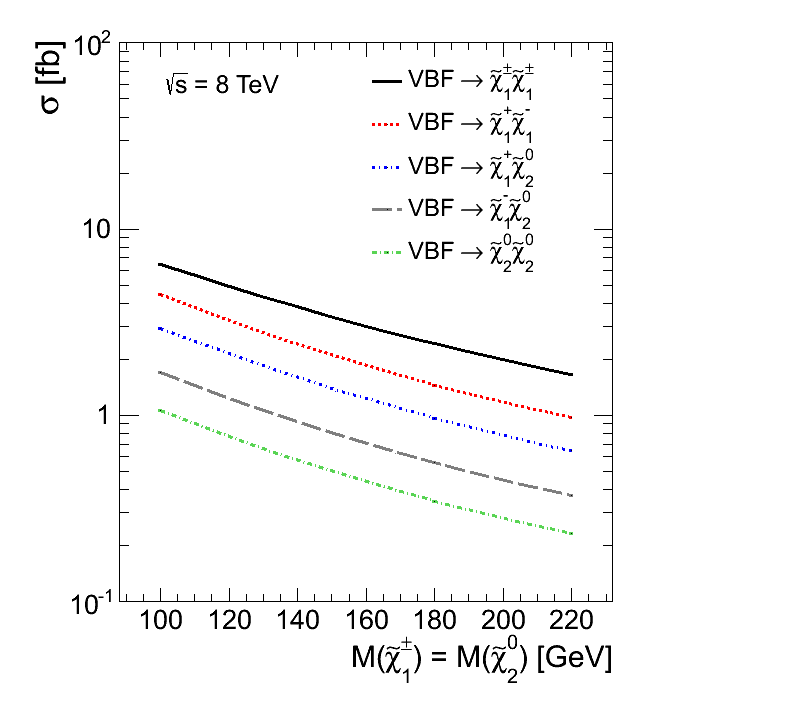
\includegraphics[width=0.75\textwidth]{analysis/pics/VBFXsection.png}
	\end{tabular}
	\caption{VBF production cross-section at \CM = 8 \tev as a function of mass for various channels after imposing \ensuremath{\deltaeta > 4.2} using Madgraph 4 \cite{Dutta:2012xe}.}
	\label{fig:VBF_xsec}
\end{figure}

The cross-section prediction for those processes are summarized in Figure \ref{fig:VBF_xsec} as function of the \charginomp - \neutralinotwo mass.

The search strategy can be divided in two distinct parts: the first one considers the kinematic of the jets produced via VBF in order to reduce the contribution coming  from V + jets events (where V is ether the W or Z boson); the second one takes into account the properties of the supersymmetric particles falling into the inner region of the detector (centrally produced) in order to reduce the all the non-supersymmetric background contributions.

The main feature of VBF processes is the production of two jets aimed at the forward-backward region of the detector with high \pt and large \deltaeta. By adding to the event selection the requirements on the di-jet \deltaeta as well as the di-jet invariant mass \ensuremath{m_{j_{1}j_{2}}} the background contribution coming from V+jets and \ttbar events is kept under control. In order to generate super-symmetric particles, the incoming partons need to have an high momentum, therefore the leading jet from the VBF-produced di-jet pair is expected to have high \pt. The addition of a \pt cut on leading jets keeps further reduces background contributions. Figure \ref{fig:VBF_mjj_ptj1} shows an early study on \ensuremath{m_{j_{1}j_{2}}} and leading jet \pt distributions for for \charginopm \charginopm pair production by VBF processes, V+jets background, and VV background produced by VBF processes.

\begin{figure}[tbh!]
	\centering
	\begin{tabular}{cc}
		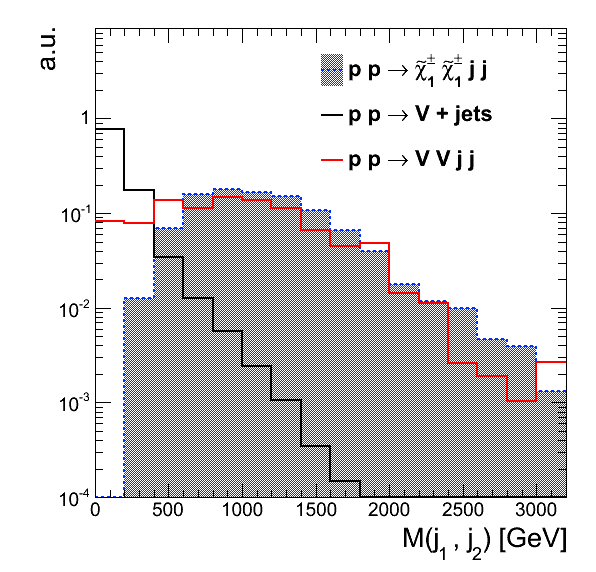
\includegraphics[width=0.50\textwidth]{analysis/pics/VBFDiJetMass.png}
		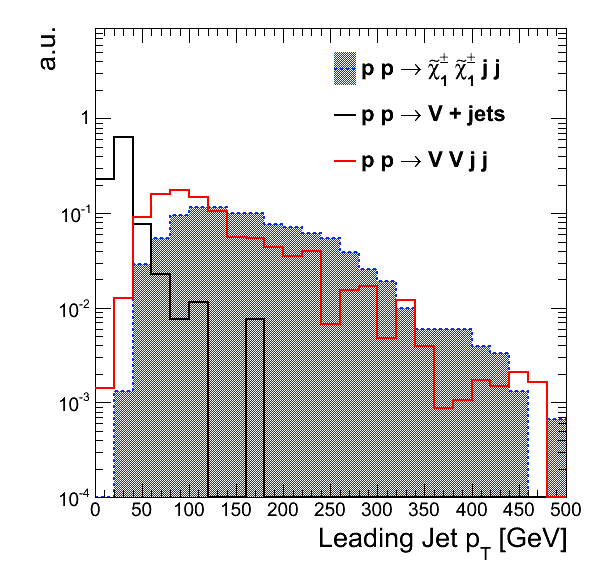
\includegraphics[width=0.50\textwidth]{analysis/pics/VBFFirstLeadingJetPt.png} 		
	\end{tabular}
	\caption{\ensuremath{m_{j_{1}j_{2}}} (left) and \pt of the leading jet (right) distributions normalized to arbitrary units for \charginopm \charginopm pair production by VBF processes, V+jets background, and VV background produced by VBF processes \cite{Dutta:2012xe}.}
	\label{fig:VBF_mjj_ptj1}
\end{figure}


The remaining background contributions come from all the centrally produced particles. By considering an R-parity conserving model the decay of \charginopm and \neutralinotwo is the following

\begin{equation}
 \charginopm \longrightarrow \stau^{\pm} \nu \longrightarrow \tau^{\pm} \neutralinoone \nu
\end{equation}

\begin{equation}
\neutralinotwo \longrightarrow \stau^{\pm} \tau^{\mp} \longrightarrow \tau^{\pm} \tau^{\mp} \neutralinoone
\end{equation}

The \neutralinoone LSP travels through the detector undetected increasing \met. The processes that mimics signal are all the VV (where V may be wither W or Z) pairs produced via VBF where the bosons decays leptonically. A \met cut is effective in reducing this background as shown on Figure \ref{fig:VBF_met_pttau}. Moreover, requiring multiple $\tau$’s in the event further reduces background. The \pt of the \ensuremath{\tau} coming from the \charginopm and \neutralinotwo decays is strongly correlated to the mass difference between the \charginopm and the \neutralinoone LSP. In Figure \ref{fig:VBF_met_pttau}, the normalized distribution of the \pt of \ensuremath{\tau} is displayed for \ensuremath{\Delta M = m_{\charginopm} - m_{\neutralinoone} =} 30 \gev and 15 \gev. For smaller \ensuremath{\Delta M}, the distribution peaks at lower \pt and the signal acceptance is less efficient.

\begin{figure}[tbh!]
	\centering
	\begin{tabular}{cc}
		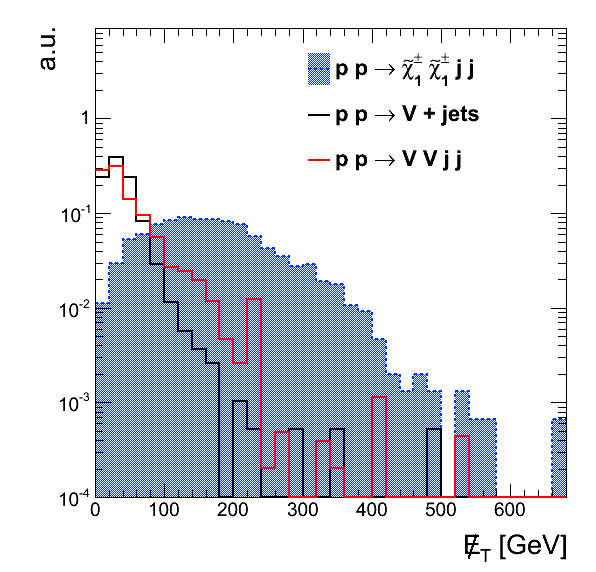
\includegraphics[width=0.50\textwidth]{analysis/pics/VBFMet.png}
		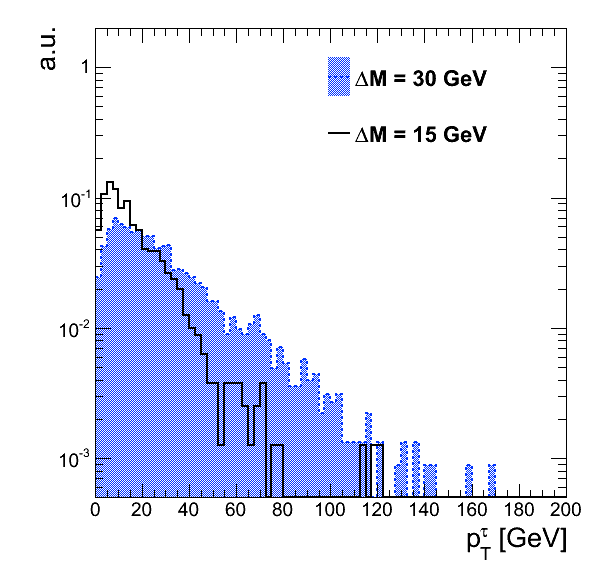
\includegraphics[width=0.50\textwidth]{analysis/pics/Pheno_VBF_TauPt.png} 		
	\end{tabular}
	\caption{(left) \met distribution normalized to arbitrary units for \charginopm \charginopm pair production by VBF processes, V+jets background, and VV background produced by VBF processes. (right) \pt of \ensuremath{\tau} distribution normalized to arbitrary units in \ensuremath{\geq 2j + 2\tau} final state for \ensuremath{\Delta M = m_{\charginopm} - m_{\neutralinoone} =} 30 \gev and 15 \gev.}
	\label{fig:VBF_met_pttau}
\end{figure}


\cleardoublepage

\chapter{Objects Reconstruction}
\label{sec:VBFSUSY}

%TODO{connect your sentences (look up sentence connectors)}
	
%TODO{browse the web about how to write introductions}
	
	%TODO{you have too much text per page :-)}
	%TODO{For a more professional look and a better reading experience: make your font large enough, make the distance between lines large enough, put some extra distance between paragraphs.}

%TODO{where do you cover track reconstruction, local calorimeter reconstruction, local muon reconstruction?}

%TODO{I recommend to move the information of this chapter as follows:}
	
%TODO{	- General information about particle reconstruction, (reconstruction algorithms and reconstruction quality) belongs to the chapter about CMS. }
	
%TODO{	The description of the specific object definitions you employed belong to the analysis chapter.}
	
%TODO{	A simpler title would simply be: particle reconstruction}

%TODO{start this chapter section by explaining what is to be accomplished, like studying final states of collisions, and what the strategy is, like reconstruction of all particles in the final state, which allows doing jets, letpon isolation, …}

The final aim of the CMS detector is the study of collision final states and several are the steps needed to transform the raw detector hits into useful information for an high energy physics analysis. The CMS collaboration converged its effort into a complex software algorithm, called Particle Flow, that combines all the information coming from all the experiments sub-detectors and reconstructs all the final state basic objects. Those reconstructed object ranges from simple particles such as electrons and muons to complex ones such as jets and hadronic taus. Particle Flow also reconstructs variables useful in the analysis selection such as jets imbalance and missing tranverse momentum. After a brief introduction on the Particle flow algorithm this chapter will give further information on the reconstruction on the most important objects used in the analysis described in this thesis.

\section{The Particle Flow Algorithm}

The raw data collected by the CMS experiment is the input of a detailed offline reconstructions of the collision final states. CMS developed over the years an algorithm, called the Particle Flow (PF) \cite{CMS:2009nxa,CMS:2010byl}, that attempts to identify and to reconstruct the kinematic properties of each of the particles in the final states. For this purpose all the information coming from each of the CMS subdetectors is combined. This algorithm heavily relies on the precise measurement of the momenta of charged particles with the silicon tracker, and the precise measurement of photon and electron energies with the highly granular and hermetic ECAL, to overcome the coarser granularity of the HCAL. The reconstructed particles are then used to reconstruct jets, \hadtau candidates, and the vector imbalance in transverse momentum in the event, referred to as \ptvecmiss, as well as to quantify the isolation of leptons. 

\subsection{Primary Vertices}
\label{subsec::objsel_vertex}

%TODO{belongs to event reconstruction in the CMS chapter}

The determination of collisions Primary Vertices (PV) for each of the bunch crossing is critical for reducing pile up effects and to detect long lived particles such as specific mesons. CMS reconstructs PVs starting from the vertices of all well reconstructed charged particle tracks in the event \cite{CMS-PAS-TRK-10-005}. The first step consist on clustering the tracks according to the position on the z-axis of their closest track segment with respect to the beam line \cite{CMS-IN-2011-014}. Then, a PV is reconstructed from each cluster with two or more constituents using a dedicated fit procedure. Which PV corresponds to the hardest interaction in the event is determined based on the tracks associated to the PV. The transverse momenta of all tracks associated to the PV are summed and the vertex with the highest sum is chosen. Every event used in this analysis requires at least a reconstructed PV. Table~\ref{table:vertexobjdefinition} shows the detailed selection criteria for such requirement.

\subsection{Electrons reconstruction}

Electrons are reconstructed by matching tracks in the inner detector with energy depositions in the ECAL \cite{CMS:2009nxa,Baffioni2007}. The tracks of electron candidates are reconstructed using a Gaussian sum filter \cite{Adam:2005bya} algorithm, which accounts for the emission of bremsstrahlung photons along the electron trajectory. Energy loss in bremsstrahlung is reconstructed by searching for energy depositions in the ECAL located in directions tangential to the electron track. A multivariate approach based on boosted decision trees (BDT) \cite{Hocker:2007ht} is employed for electron identification \cite{1748-0221-10-06-P06005}.

\subsection{Muons reconstruction}

 The identification of muons is based on linking track segments reconstructed in the silicon tracking detector and in the muon system \cite{Chatrchyan:2012xi}. The matching between track segments is done outside-in, starting from a track in the muon system, and inside-out, starting from a track reconstructed in the inner detector. In case a link can be established, the track parameters are refitted using the combined hits in the inner and outer detectors, with the resulting track referred to as a global muon track. Quality criteria are applied on the multiplicity of hits, on the number of matched segments, and on the fit quality of the global muon track, quantified through a \ensuremath{\chisquare}.

\subsection {The Jet reconstruction}
\label{subsec::objsel_bjet}
\label{subsec::objsel_jet}

%TODO{Jet reconstruction does not belong to the particle flow algorithm. Probably you want to have the section about jets in the object definition section of your analysis chapter. You might want a few words and figures about jets in the particle reconstruction section of the CMS section}

Jets within the range \ensuremath{|\eta| < 4.7} are reconstructed using the anti-\ensuremath{k_{T}} algorithm \cite{antikt} with a distance parameter of 0.5. As mentioned previously, the particles reconstructed by the PF algorithm are used as input to the jet reconstruction. Reconstructed jets are required not to overlap with identified electrons, muons, or \hadtau within \ensuremath{\deltar < 0.5}, and to pass two levels of jet identification criteria: (i) misidentified jets, mainly generating from calorimeter noise, are rejected by requiring reconstructed jets to pass a set of loose jet identification criteria \cite{CMS:2010xta} and (ii) jets originating from pileup interactions are rejected through an MVA-based jet identification discriminant, based on information about the vertex and energy distribution within the jet \cite{CMS:2013wea}. 

The energy of reconstructed jets is calibrated as a function of jet \pt and \ensuremath{\eta} \cite{1748-0221-6-11-P11002}. The contribution of pileup to the energy of jets originating from the hard scattering is compensated by determining a median transverse momentum density (\ensuremath{\rho}) for each event, and subtracting the product of (\ensuremath{\rho}) times the area of the jet, computed in the \ensuremath{\eta-\Phi} plane, from there constructed jet \pt \cite{Cacciari:2008gn, Cacciari:2007fd}. 

Particle Flow jets (PFJets) are used in this analysis. The \antikt clustering algorithm with a reconstruction cone of \ensuremath{R = 0.5} is used, defined in \ensuremath{\eta-\phi (R = \sqrt{{\Delta \eta}^2 + {\Delta \phi}^{2}})} \cite{1126-6708-2008-04-063}. 

The PF jets used in this analysis are corrected using L1 FastJet, L2 Relative, and L3 Absolute corrections. The L1 FastJet corrections use the event-by-event UE/PU (Underlining Events / Pile Up) densities to remove the additional contributions to the measured jet energies due to underlying event and pile-up particles. The L2 and L3 corrections use jet balancing and \ensuremath{\gamma} + jets events to improve and provide a better energy response as a function of \pt and \ensuremath{\eta}. This analysis uses the "loose" working point Jet-Id selection criteria jets \pt = 30 \gev and absolute pseudorapidity $|\eta| \le 5.0$. Table~\ref{table:bjetobjdefinition} shows the detailed selection criteria used for the recommended loose working point. The efficiency is $> 98$ for the entire $\eta$ and \pt range. The "loose'' working point has been validated in other studies.

Jets originating from the hadronization of b quarks are identified through the combined secondary vertex (CSV) algorithm \cite{Chatrchyan:2012jua}, which exploits observables related to the long lifetime of b hadrons and the higher particle multiplicity and mass of b jets compared to light-quark and gluon jets. This analysis uses the loose working point of the combined secondary vertex algorithm \cite{CMS:2011cra}. The EPS13 prescription is used for the b-tagging and mis-tagging scale factors and efficiencies. They are applied using the method called ``Event reweighing using scale factors only" \cite{Ferencek:btag2015}. Table~\ref{table:bjetobjdefinition} shows the detailed selection criteria.


%TODO{MET and MET-like variables belong to the object definition section of the analysis chapter} 
	
%TODO{	you say MET and \ensuremath{|sum p_T^jet|} are  the same, while they are not}	
%TODO{	besides, MET does not belong to a section  named “jet reconstruction”}
%TODO{	do you use the multivariate technique in [26]? if not don’t mention it}

\subsection {\met reconstruction}
\label{subsec::objsel_met}

Two algorithms are used to reconstruct \ptvecmiss, the imbalance in transverse momentum in the event, whose magnitude is referred to as \met. The standard algorithm computes the negative vectorial sum of all particle momenta reconstructed using the PF algorithm. In addition, a multivariate regression algorithm \cite{Khachatryan:2014gga} has been developed to reduce the effect of pileup on the resolution in \met. The algorithm utilizes the fact that pileup predominantly produces jets of low \pt, while leptons and high-\pt jets are produced almost exclusively in the hard-scatter.

Detection of weakly interacting particles is crucial both for SM measurements and searches for new physics. Although such particles leave no trace in any of CMS’s subdetectors, their transverse momenta can be estimated as the missing transverse energy in the event, making use of momentum conservation:

\begin{equation}
\met =  - \sum_{j} \pt^{j}
\end{equation}

where \ensuremath{\pt^{j}} is the transverse momentum of PF particle j. Figure \ref{fig:true_met} shows the energy and \ensuremath{\phi} resolution of the reconstructed \met in simulation versus the true \met. Again, the PF approach is compared to the calorimetric-based approach and performs substantially better. Table~\ref{table:metobjdefinition} shows the detailed selection criteria.

\begin{figure}[tbh!]
	\centering
	\begin{tabular}{cc}
		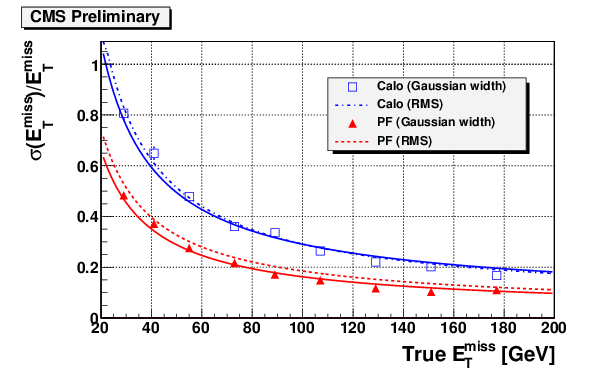
\includegraphics[width=0.48\textwidth]{objreconstruction/pics/true_met-a.png}
		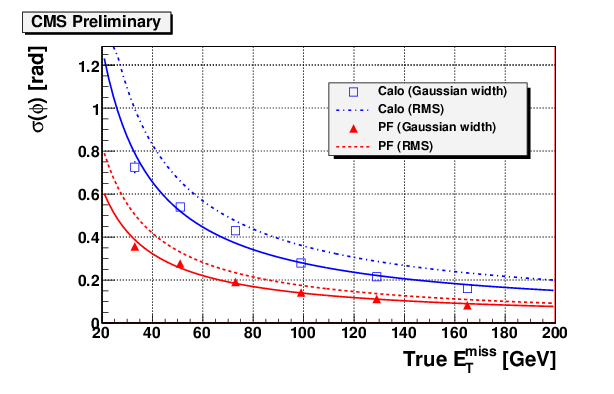
\includegraphics[width=0.48\textwidth]{objreconstruction/pics/true_met-b.png} 		
	\end{tabular}
	\caption{The energy and \ensuremath{\phi} resolution of the \met in simulation. Red triangles show the resolution for the PF approach. Blue squares show the resolution for the calorimetric approach. The full lines show the results of fits of the data points and the dashed lines show the results of fits of an alternative resolution measure \cite{CMS:2009nxa}}
	\label{fig:true_met}
\end{figure}

\clearpage

\section {Tau lepton reconstruction}
\label{subsec::objsel_tau}

The $\tau$ lepton was discovered between 1974 and 1977 by the team under Martin Perl at SLAC/SPEAR while studying the $e^{+}+e^{-}\longrightarrow e^{\pm}+\mu^{\mp}$ \cite{Perl:1975bf}. With a mean lifetime of $2.9\times10^{-13}$ s and a mass of 1776.82 \mev \cite{Agashe:2014kda} it is the heaviest of the leptons, enough to decay into hadrons, and it does so in about two thirds of the cases, typically into either one, three or five charged pions or kaons and up to four neutral pions \ensuremath{\pi^{0}}, and one neutrino \ensuremath{\nu_{\tau}}. The \ensuremath{\pi^{0}} meson decays almost exclusively into \ensuremath{\gamma\gamma}. Among all the possible hadronic decays as shown on Table \ref{table:tau_hdecay} the ones called "one-prong", where only one charged hadron is produced, are the most frequent. The $\tau$ decays also leptonically, with a branching ratio of $17\%$ for each channel, via the following decay $\tau\longrightarrow\nu_{\tau}W^{*}\longrightarrow\nu_{\tau}l\nu_{l}$.

\begin{figure}[tbh!]
	\begin{center}	
		\begin{tabular}{ | c | c | c | c |}
			\hline
			Decay Mode & Resonance & Mass [\mev] & BF (\%) \\ \hline
			\hline
			$\tau^{-}\longrightarrow h^{-}\nu_{\tau}$& $\pi$ & 139.6 & 11.6 \\ \hline
			$\tau^{-}\longrightarrow h^{-}\pi^{0}\nu_{\tau}$& $\rho$ & 770 & 26.0 \\ \hline
			%				$\tau^{-}\longrightarrow h^{-}\pi^{0}\pi^{0}\nu_{\tau}$ & $a_{1}$ & 1200 & \\ 10.8 \hline
			$\tau^{-}\longrightarrow h^{-} h^{+} h^{-} \nu_{\tau}$& $a_{1}$& 1200 & 9.8 \\ \hline
			$\tau^{-}\longrightarrow h^{-} h^{+} h^{-} \pi^{0}\nu_{\tau}$& & & 4.8 \\ \hline
			other hadronic channels& & & 1.7 \\ \hline
			\hline
			total & & & 64.8 \\ \hline
		\end{tabular}
		\caption{ Hadronic tau decay modes into either one or three charged hadrons h and potential $\pi_{0}$, and the corresponding branching fractions BF. Also shown are the intermediate resonances and their masses, which are used in some of the tau reconstruction algorithms \cite{Agashe:2014kda}.}
		\label{table:tau_hdecay}
	\end{center}
\end{figure}

The \hadtau decays are reconstructed and identified using the hadrons-plus-strips (HPS) algorithm \cite{Chatrchyan:2012zz}, a cut-based algorithm focusing on the reconstruction of neutral pions. The HPS algorithm is seeded by jets of \ensuremath{\pt > 14 \gev} and \ensuremath{|\eta| < 2.5}, reconstructed using the anti-\ensuremath{k_{T}} algorithm \cite{antikt} with a distance parameter of 0.5. The algorithm is designed to reconstruct individual decay modes of the \ensuremath{\tau} lepton, taking advantage of the excellent performance of the PF algorithm in reconstructing individual charged and neutral particles.
The reconstruction and identification of \hadtau decays in the HPS algorithm is performed in two steps:

\begin{itemize}
	\item \textbf{Reconstruction:} combinations of charged and neutral particles reconstructed by the PF algorithm that are compatible with specific \hadtau decays are constructed, and the four-momentum, expressed in terms of (\pt, \ensuremath{\eta}, \ensuremath{\phi} , and mass) of \hadtau candidates, is computed.
	
	\item \textbf{Identification:} discriminators that separate \hadtau decays from quark and gluon jets, and from electrons and muons, are computed. This provides a reduction in the jet \ensuremath{\longrightarrow \hadtau}, \ensuremath{e \longrightarrow \hadtau}, and \ensuremath{\mu \longrightarrow \hadtau} misidentification rates.
\end{itemize}

\subsection{Identification of decay modes}

Reconstruction of specific \hadtau decay modes requires reconstruction of neutral pions that are present in most of the hadronic \ensuremath{\tau} decays. The high probability for photons originating from \ensuremath{\pi^{0} \longrightarrow \gamma \gamma} decays to convert to \ensuremath{e^{+}e^{-}} pairs within the volume of the CMS tracking detector is taken into account by clustering the photon and electron constituents of the \ensuremath{\tau}-seeding jet into “strips” in the \ensuremath{\eta - \phi} plane. The clustering of electrons and photons of \ensuremath{\pt > 0.5} \gev into strips proceeds via an iterative procedure. The electron or photon of highest \pt not yet included into any strip is used to seed a new strip. The initial position of the strip in the \ensuremath{\eta - \phi} plane is set according to the \ensuremath{\eta} and \ensuremath{\phi} of the seed \ensuremath{e} or \ensuremath{\gamma}. The \ensuremath{e} or \ensuremath{\gamma} of next-highest \pt that is within an \ensuremath{\eta \times \phi} window centred on the strip location is merged into the strip. The strip position is then recomputed as an energy-weighted average of all electrons and photons contained in the strip \cite{Khachatryan:2015dfa}.

\hadtau candidates are formed by combining the strips with the charged-particle constituents of the jet. The charged particles are required to satisfy the condition \ensuremath{\pt > 0.5 \gev}. The distance of closest approach between their tracks and the hypothetical production vertex of the \hadtau candidate, taken to be the vertex closest to the charged particle of highest \pt within the jet, is required to be less than 0.4 cm in the z direction and \ensuremath{< 0.03} cm in the transverse plane. These requirements removes spurious reconstructed tracks and significantly reduces the effect of pileup.

A combinatorial approach is taken for constructing hadronic \ensuremath{\tau} candidates. Multiple \hadtau hypotheses, corresponding to combinations of either one or three charged particles and up to two strips, are constructed for each jet.

The four-momentum of each \hadtau candidate hypothesis is given by the four- momentum sum of the charged particles and strips. In a few per cent of the cases, the charged particles included in the \hadtau candidates are identified as electrons or muons, and are assigned their respective electron or muon masses by the PF algorithm. The HPS algorithm sets the mass of all charged particles included in \hadtau candidates to that of the charged pion, except for electron constituents of strips, which are treated as massless. The charge of \hadtau candidates is reconstructed by summing the charges of all particles included in the construction of the \hadtau candidate, except for the electrons contained in strips. The probability for mis-reconstructing the \hadtau charge is \ensuremath{\approx 1 \%}, with a moderate dependence on \pt and \ensuremath{\eta}, for taus from Z decays.

\begin{figure}[tbh!]
	\centering
	\begin{tabular}{cc}
		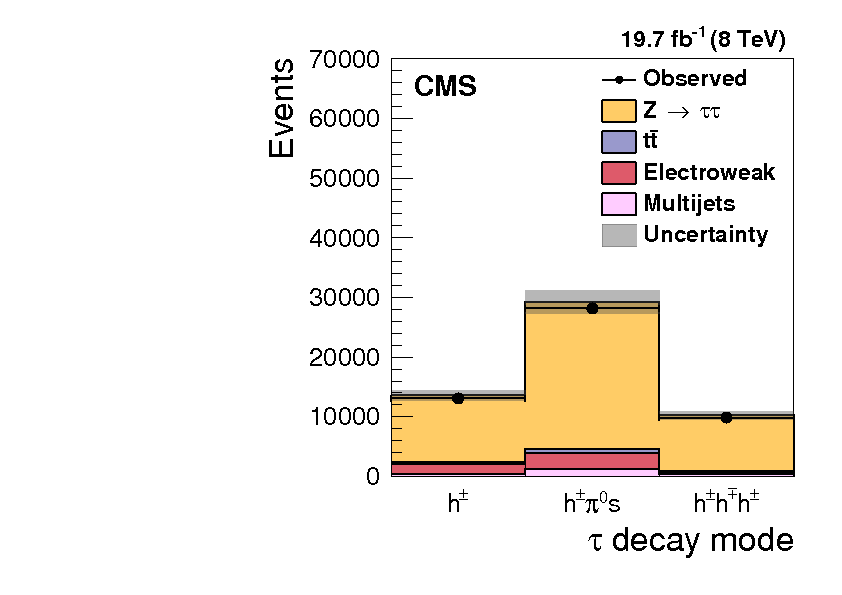
\includegraphics[width=0.5\textwidth]{objreconstruction/pics/scalefactors050314.png}
		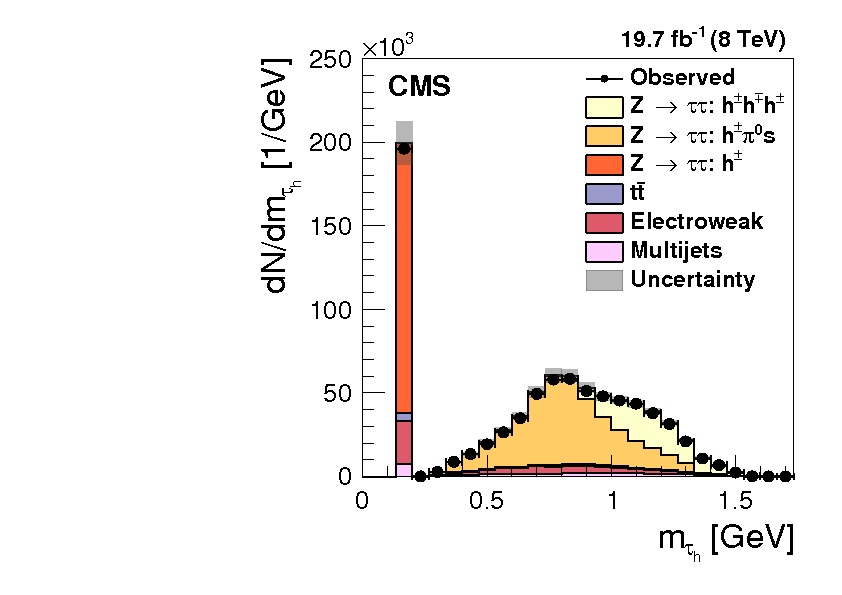
\includegraphics[width=0.5\textwidth]{objreconstruction/pics/plots_paper_tauIdAlgorithm_ZTT_mTau_ZTT_linear.png} 		
	\end{tabular}
	\caption{Contributions in reconstructed \hadtau decay modes  (left) and \hadtau candidate masses in \ensuremath{Z/\gamma^{*} \longrightarrow \tau\tau}  events selected in data (right), compared to MC expectations. The \ensuremath{Z/\gamma^{*} \longrightarrow \tau\tau}  events are selected in the decay channel of muon and \hadtau \cite{Khachatryan:2015dfa}.}
	\label{fig:Ztautau_decaymodes}
\end{figure}

The following criteria are applied to assure the compatibility of each hypothesis with the signatures expected for the different \hadtau decays in Table \ref{table:tau_hdecay}:

\begin{enumerate}
	\item \ensuremath{h^{\pm}h^{\pm}h^{\pm}}: Combination of three charged particles with mass \ensuremath{0.8 < m_{\hadtau} < 1.5 \gev}. The tracks are required to originate within \ensuremath{\Delta z < 0.4} cm of the same event vertex, and to have a total charge of one.
	\item \ensuremath{h^{\pm}\pi^{0}\pi^{0}}: Combination of a single charged particle with two strips. The mass of the \hadtau candidate is required to satisfy the condition \ensuremath{0.4 < m_{\hadtau} < 1.2 \sqrt{\pt [\gev]/100}}\gev. The size of the mass window is enlarged for \hadtau candidates of high \pt to account for resolution effects. The upper limit on the mass window is constrained to be at least 1.2 and at most 4.0 \gev.
	\item \ensuremath{h^{\pm}\pi^{0}}: Combination of one charged particle and one strip with mass \ensuremath{0.3 < m_{\hadtau} < 1.3 \sqrt{\pt [\gev]/100}}\gev. The upper limit on the mass window is constrained to be at least 1.3 and at most 4.2 \gev.
	\item \ensuremath{h^{\pm}}: A single charged particle without any strips.
\end{enumerate}

The combinations of charged particles and strips considered by the HPS algorithm represent all hadronic \ensuremath{\tau} decay modes in Table \ref{table:tau_hdecay}, except \ensuremath{τ^{-} \longrightarrow h^{-}h^{+}h^{-}\pi^{0}\nu_{\tau}}. The latter corresponds to a branching fraction of \ensuremath{4.8\%} and is not considered in the present version of the algorithm, because of its contamination by jets. The \ensuremath{h^{\pm}\pi^{0}} and \ensuremath{h^{\pm}\pi^{0}\pi^{0}} decays are analyzed together, and referred to as \ensuremath{h^{\pm}\pi^{0}s}.

Hypotheses that fail the mass window selection for the corresponding decay mode are discarded. When multiple combinations of charged hadrons and strips pass the mass window and the signal cone requirements, the hypothesis for the candidate with largest \pt is retained. All other combinations are discarded, resulting in a unique \hadtau candidate to be associated to each jet.

The contributions in the decay modes and in the mass of \hadtau candidates in \ensuremath{Z/\gamma^{*} \longrightarrow \tau\tau} events are shown in Figure \ref{fig:Ztautau_decaymodes}. The contribution of the \ensuremath{Z/\gamma^{*} \longrightarrow \tau\tau} signal is split according to the reconstructed \hadtau mode, as shown in the legend. For \hadtau candidates reconstructed in the \ensuremath{h^{\pm}\pi^{0}s} and \ensuremath{h^{\pm}h^{\pm}h^{\pm}} modes, the \ensuremath{m_{\hadtau}} distribution peaks near the intermediate \ensuremath{ρ\rho(770)} and \ensuremath{a_{1}(1260)} meson resonances (cf. Table \ref{table:tau_hdecay}), as expected. The narrow peak at the charged pion mass is due to \hadtau candidates reconstructed in the \ensuremath{h^{\pm}} mode.

\subsection{Isolation}

Requiring reconstructed \hadtau candidates to pass strict isolation requirements constitutes the main handle for reducing the large multijet background \cite{Khachatryan:2015dfa}. Tau leptons are usually isolated relative to other particles in the event, and so are their decay products, in contrast to quark and gluon jets. Two types of \hadtau isolation discriminants have been developed, using simple cutoff-based selections and an MVA approach. The expected efficiency of the \hadtau isolation discriminants in \ensuremath{Z/\gamma^{*} \longrightarrow \tau\tau} events ranges from \ensuremath{49.0\%} (Loose) to \ensuremath{38.1}\% (Tight) for the cutoff-based approach and \ensuremath{55.9\%} (Very Loose) to \ensuremath{27.3\%} (Tight) for the MVA one. The Jet \ensuremath{\to \tau} misidentification rate of the \hadtau isolation discriminants in Multi-jet events ranges from \ensuremath{3.86 \times 10^{-3}} (Loose) to \ensuremath{1.75 \times 10^{-3}}\% (Tight) for the cutoff-based approach and \ensuremath{6.21 \times 10^{-3}} (Very Loose) to \ensuremath{4.43 \times 10^{-3}} (Tight) for the MVA one.
 
\subsection{Electron and Muon veto}

Electrons and muons have a sizable probability to get reconstructed in the \ensuremath{h^{\pm}} decay mode. Electrons radiating a bremsstrahlung photon that subsequently converts may also get reconstructed in the \ensuremath{h^{\pm}\pi^{0}s} decay mode. In particular, electrons and muons originating from decays of W and Z bosons, which are produced with cross sections of \ensuremath{\approx100} nb at the LHC at \ensuremath{\sqrt{s} = 8} \tev have a high chance to pass isolation-based \hadtau identification criteria. Dedicated discriminants have been developed to separate \hadtau from electrons and muons \cite{Khachatryan:2015dfa}. The separation of \hadtau from electrons is based on an MVA approach, with an efficiency and \ensuremath{e\to \tau} misidentification rate going from \ensuremath{93.3\%} and \ensuremath{2.38 \times 10^{-2}} (Very loose) to \ensuremath{72.1\%} and \ensuremath{3.54 \times 10^{-4}} (Very tight) in \ensuremath{Z/\gamma^{*} \longrightarrow \tau\tau} events.
A cut based and an MVA based discriminant are used to separate \hadtau from muons. The expected efficiency of the \hadtau against muon discriminants in \ensuremath{Z/\gamma^{*} \longrightarrow \tau\tau} events goes from \ensuremath{99.3\%} (Loose) to \ensuremath{99.1}\% (Tight) for the cutoff-based approach and \ensuremath{99.5\%} (Loose) to \ensuremath{98\%} (Tight) for the MVA one. The \ensuremath{\mu \to \tau} misidentification rate efficiency of the \hadtau isolation discriminants in \ensuremath{Z/\gamma^{*} \longrightarrow \mu\mu} events ranges from \ensuremath{1.77 \times 10^{-3}} (Loose) to \ensuremath{7.74 \times 10^{-4}} (Tight) for the cutoff-based approach and \ensuremath{5.20 \times 10^{-4}} (Loose) to \ensuremath{3.18 \times 10^{-4}} (Tight) for the MVA one.

\hadtau candidates are required to have a \pt of 45 \gev and a pseudo-rapidity of $|\eta| \le 2.1$ in order to ensure that both tracks are reconstructed fully within the acceptance of the tracking system. In addition, a \hadtau is required to have exactly one signal charged hadron with \pt = 5 \gev and must not reside in the ECAL cracks.

One-prong \hadtau candidates are selected using the \texttt{Decay\-Mode\-Finding\-New\-DMs} discriminator. In order to discriminate against muons, HPS taus are required to pass the \texttt{against\-Muon\-Loose3} rejection discriminator which requires the lead track of the tau not be associated with a global muon signature. In order to discriminate against electrons, HPS taus are required to pass the \texttt{against\-Electron\-Medium\-MVA5} discriminator which uses the amount of HCAL energy associated to the tau with respect to the measured momentum of the track. Additionally, the MVA discriminator considers the amount of electromagnetic energy in a narrow strip around the leading track with respect to the total electromagnetic energy of the tau. 

The isolation discriminator is a BDT \cite{Hocker:2007ht} discriminator based on isolation, \pt and \hadtau lifetime information and defines the different TauID working points starting from the loose one with (\texttt{byLoose\-Isolation\-MVA3\-newDMwLT}) to the tighter one (\texttt{byTight\-Isolation\-MVA3new\-DMwLT}). Table~\ref{table:bjetobjdefinition} shows the detailed selection criteria for an \hadtau candidate.


\clearpage
\cleardoublepage

\chapter{Search for VBF SUSY in the di-$\hadtau$ Like Sign channel}
\label{sec:analysis}
%TODO You need a small introduction here. The reader needs to get an idea or be reminded of what to expect. Probably 7 - 10 lines and at most half a page.

%TODO start with data+trigger and mc samles, then have the object definitions, then have the event selection

\section{Event Selection}
\label{sec:eventselection}

%TODO one topic per paragraph

%TODO read it again and try to make your text easier to understand for a reader that is less familiar with LHC analyses

As mentioned in Section \ref{section::search_strategy} the di-\hadtau channel's main background contribution comes from QCD multijet, with a rate several orders of magnitude larger than the rate in other contributions.  Hence this search channel, more than any of the others, relies on the efficient background rejection. Fortunately, the VBF and \met selections provide the required background suppression.

All the collision data events passing the requirements of the triggers shown on Table \ref{table:triggerdefinition} are considered as the interesting events for offline analysis. 

As previously introduced in Section \ref{section::search_strategy}, the event selection criteria is divided in two distinct parts: the central part, which takes into account the LSP and the decay products of the multiple \hadtau, and the VBF part, which cuts over the kinematic properties of the jets coming from a VBF process. 

The main differences with the other VBF SUSY searches with final states to light leptons, are the substantially tighter \hadtau requirements targeting at the suppression of QCD jet background and the looser missing transverse energy (\met) requirement, to recover some of the signal acceptance lost due to the larger discriminator based on isolation $\hadtau$ \pt thresholds needed to stay efficient with respect to the trigger.  

%TODO Higher multiplicity t_h: I understand what you mean, but most readers won’t

The selected events are required to have at least two \hadtau candidates as defined in Section \ref{subsec::objsel_tau}. Higher multiplicity \hadtau are constrained by the trigger. The like sign \hadtau candidates with the highest \pt and separated from each other by a minimum \deltar = 0.3 are then chosen to form a di-\hadtau candidate. 
Further, to reduce top pair contamination the event is required not to have any jet identified as a b--quark jet by the b--tagging algorithms using the {\textit combined secondary vertex loose} (CSVL) working point. 

Only jets with \pt $\ge 30\gev$ and separated from the taus in the di--\hadtau pairs by $\Delta R \ge 0.3$ are searched for b--tags. The higher \pt cut of 30\gev on b-jets (a looser veto requirement than other analyses with light leptons) allows us to be more efficient with respect to the signal since the higher \pt threshold on taus reduces the contamination of $t\overline{t}$ to a large extent. Further, the event is required to have at least 30\gev of \met. All the above described selections is what will be referred as {\textit central selections}.

Subsequently, the following event-wide requirements are imposed. The {\textit {VBF selections}} are imposed by requiring at least two jets as defined in Section \ref{subsec::objsel_jet}. Only jets separated from the leptons in the \hadtau\hadtau pair by $\deltar \ge 0.3$ are considered. All jet candidates passing the above requirements and having $\vert \Delta\eta \vert \ge 4.2$ and $\eta_{1}\cdot\eta_{2} < 0$ are combined to form di-jet candidates. The final and the most important of the requirement is an invariant mass of the di-jet candidate, namely \mjj, above the threshold of 250\gev. In order to increase the event acceptance the analysis code algorithm takes into account every possible di-jet candidate combination and chooses the one that passes the VBF requirements and has the highest \mjj. 

For better visualization and understanding all the selection criteria are summarized the following way:

%TODO it’s more elegant to have this in a table instead of a bullet list.

\begin{itemize}
	\item \textbf{Central selection}
	\begin{itemize}
		\item Trigger: \texttt{HLT\_DoubleMediumIsoPFTau35\_Trk*\_eta2p1\_Prong1\_v*}
		\item two one-prong hadronically decaying $\tau$ with $\pt\geq45~$\gev 
		\item $\met > $ 30
		\item at least two jets with $p_{T}^{jet}\geq30~$\gev, $|\eta_{jet}|\leq5$ and loose jetID
		\item $\Delta R(jet,\tau)\geq0.3$
		\item b-tag veto
	\end{itemize}
	\item \textbf{VBF selection}
	\begin{itemize}
		\item $|\Delta\eta(jet,jet)| > 4.2$
		\item $sign(\eta^{jet 1}\cdot\eta^{jet 2})==-1$
		\item $\mjj>250~$\gev
	\end{itemize}
\end{itemize}

%todo you need a cutflow table here, and a discussion about how event yields for data and MC samples reduces with cuts.

\clearpage



\section{Signal and Background Samples}

%TODO first you need a section about data and trigger

%TODO you need to explain more precisely where MC is used: signal prediction, *part* of the bkg prediction, optimization, design of QCD background prediction

%TODO you use “normalize” for 2 different things. Rephrase to make clear  - that you *normalize* the MC yields to the integrated luminosity of the data (quote number) - *by using* cross sections predicted with …  

The background yields are taken from simulation. Simulated samples of signal and background events are generated using Monte Carlo (MC) event generators.

 The signal event samples are generated with the \texttt{MadGraph v5.1.5} program \cite{Alwall:2011uj}, considering pair production of gauginos with two associated partons. The signal events are generated requiring a pseudorapidity gap $|\deltaeta| > 4.2$ between the two partons, with $\pt > 30$ \pt for each parton. Signal cross sections are calculated at leading order using the MadGraph generator. The range of signal cross sections is $50^{–1}$ fb for \charginopm = \neutralinotwo masses of 100–-300\gev.
 
 Background event samples with a Higgs boson produced through VBF processes, and single top are generated with the \texttt{POWHEG v1.0r1380} program \cite{Frixione:2007vw}. 
 The \texttt{MadGraph v5.1.3} generator is used to describe Z+jets, W+jets, tt, di-boson, and VBF Z boson production. The MC background and signal yields are normalized to the integrated luminosity of the data. 
 The \ttbar background is normalized to the next-to-next-to-leading-logarithm level using the calculations of references \cite{Czakon:2013goa,Melnikov:2006kv}. 
 The Z+jets and W+jets processes are normalized to next-to-next-to-leading-order using the results from the \texttt{FEWZ v2.1} \cite{Gavin:2010az} generator. 
 The di-boson background processes are normalized to next-to-leading-order using the \texttt{MCFM v5.8} \cite{Campbell:2010ff} generator, while the VBF Z boson events are normalized to next-to-leading order using the \texttt{VBFNLO v2.6} \cite{Arnold:2008rz,Arnold:2011wj}program. 
 The single-top and VBF Higgs boson background yields are taken from the powheg program, where the next-to-leading order effects are incorporated.
 
  All MC samples incorporate the \texttt{CTEQ6L1} \cite{Pumplin:2002vw} or \texttt{CTEQ6M} \cite{Nadolsky:2008zw} parton distribution functions (PDF). The corresponding evaluation of uncertainties in the signal cross sections is discussed in Section \ref{sec:systematics}. The \texttt{POWHEG} and \texttt{MadGraph} generators are interfaced with the \texttt{PYTHIA v6.4.22} \cite{Sjostrand:2006za} program, which is used in the mathing between the matrix elements and the parton shower, and the hadronization processes. 
  
  
  The decays of $\tau$ leptons are described using the \texttt{tauola (27.1215)} \cite{Davidson:2010rw} program. The background samples are processed with a detailed simulation of the CMS apparatus using the \texttt{Geant4} package \cite{Agostinelli:2002hh}, while the response for signal samples is modeled with the CMS fast simulation program \cite{Abdullin:2011zz}. For the signal acceptance and \mjj shapes based on the fast simulation, the differences with respect to the \texttt{Geant4}-based results are found to be small ($< 5\%$). Corrections are applied to account for the differences. 
  
  For all MC samples, multiple proton-proton interactions are superimposed on the primary collision process, and events are reweighted such that the distribution of reconstructed collision vertices matches that in data. The distribution of the number of pileup interactions per event has a mean of 21 and a root-mean-square of 5.5. 
  
  For all datasets, a common \texttt{Physics Analysis Toolkit} (\texttt{PAT}) \cite{Adam:2010zza} sequence has been used to generate a PAT format, then further reduced in size by the ntuple producer \cite{bib:thentuplemaker}.

%TODO how is the trigger modeled in MC? you use the same reconstruction software on MC as on data? geant4 is not the full story: electronics and propagation of light through material is emulated (digitization step)

\section {LS di-Tau Data-Driven QCD background prediction} \label{sec:bgestimation}

%TODO improve flow of information, e.g.
%TODO 1. short introduction to the concept
%TODO 2. definition of control regions ( table with event yields)
%TODO 3. assumptions
%TODO 4. the actual method

%TODO better title (in my opinion) QCD background determination

The QCD background contribution for the like-sign di-\hadtau channel is done using a ABCD data-driven approach. This method consist in  dividing the analyzed data in different exclusive regions, defined by two variables. The first variable is the \hadtau isolation discriminator used in the object reconstruction, namely:
 	
 	%TODO don’t use these funny names here: just use “tight”, “loose” and “medium”, introduced in the object definition, with a reference such that the really interested can find back what you exactly mean. and you have the appendix anyway.
 	
 	\begin{enumerate}
 		\item Tight or T isolated $\hadtau$ for \texttt{byTight\-IsolationMVA3newDMwLT};
 		\item Medium or M isolated $\hadtau$ for \texttt{byMedium\-IsolationMVA3newDMwLT} but failed \texttt{byTight\-IsolationMVA3newDMwLT};
 		\item Loose or L isolated $\hadtau$  for \texttt{byLoose\-IsolationMVA3newDMwLT} but failed \texttt{byTight\-IsolationMVA3newDMwLT} and \texttt{byMedium\-IsolationMVA3newDMwLT}.
 	\end{enumerate}
 	
Each event with a successfully reconstructed LS di-$\hadtau$ pair falls into a exclusive isolation region as shows on Figure \ref{fig:tauisoregions}:
 	
 	\begin{itemize}
 		\item SR or signal region consisting of two tight isolated $\hadtau$;
 		\item 1T or One Tight isolated $\hadtau$ region consisting of one tight isolated $\hadtau$ and an additional medium or loose isolated $\hadtau$;
 		\item AT or Anti Tight isolation region consisting of at least one medium isolated $\hadtau$ and an additional medium or loose isolated $\hadtau$;
 		\item AM or Anti Medium isolation region consisting of two loose isolated $\hadtau$.
 	\end{itemize}
 
 	\begin{figure}[tbh!]
 		\centering
 		\begin{tabular}{cc}
 			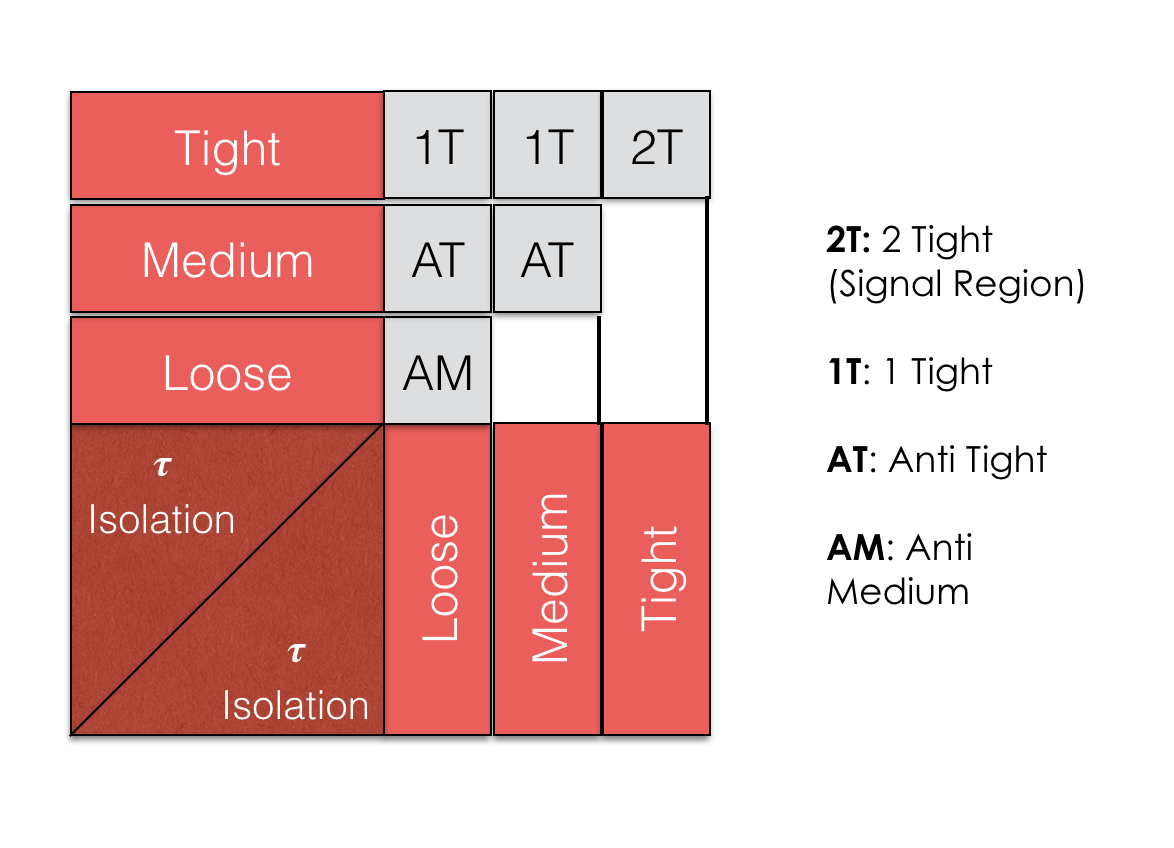
\includegraphics[width=0.75\textwidth]{PLOTS/diTauHadLSotherPlots/tauisoregions.png}
 		\end{tabular}
 		\caption{Definitions of the exclusive isolation region depending on the isolation of each of the $\hadtau$ where SR is Signal Region consisting of two tight isolated $\hadtau$, 1T is One Tight isolated Tau region consisting of one tight isolated $\hadtau$ and an additional medium or loose isolated $\hadtau$, AT is Anti Tight isolation region consisting of at least one medium isolated $\hadtau$ and an additional medium or loose isolated $\hadtau$,  AM is Anti Medium isolation region consisting of two loose isolated $\hadtau$}
 		\label{fig:tauisoregions}
 	\end{figure}
 
The second dimension of exclusivity is based on the VBF cuts described in \ref{sec:eventselection}. The regions are defined the following way:
	
	\begin{enumerate}
		\item VBF region: consisting of all the events that passed all VBF cuts previously mentioned;
		\item VBF inverted region: consisting of all the events that at least fails one of the VBF cuts previously mentioned;
	\end{enumerate} 

Using these definitions one signal region (SR) and seven control regions (CR) are defined as shown in Figure \ref{fig:crs}. The SR falls into the region defined by two tight isolated $\hadtau$ and all the VBF cuts applied, close to it the control region two (CR2) features the same \hadtau isolation requirements but inverted VBF selection requirement. In order to keep the QCD background contribution low in SR and CR2 an additional cut of  \met $ > $ 30\gev is required.

The estimation of the events in the signal region is equivalent to the classic ABCD method consisting in counting the number of events in CR2 and multiplying it with a proper conversion factor. This estimation method has been developed under the following assumptions:

\begin{itemize}
	\item[1] The VBF selection efficiency is independent from any trigger efficiency concerning $\hadtau$ isolation such that each contribution to the numerator and denominator cancels out;
	\item[2] The VBF selection efficiency is also independent from any \met cut applied in order to reduce QCD background contributions. 
\end{itemize}

 The number of   in the following equation:

\begin{equation}
N^{QCD}_{SR} = \left( N^{DATA}_{CR2} - N^{\overline{QCD} BG}_{CR2} \right) * \left[ \frac{\epsilon^{QCD}_{VBF}}{1 - \epsilon^{QCD}_{VBF}} \right]
\label{eq:qcdbgpred}
\end{equation}

where $N^{QCD}_{SR}$ is the number of QCD events predicted in the signal region, $N^{DATA}_{CR2}$ is the number of data events in CR2, $N^{\overline{QCD} BG}_{CR2}$ is the number of all non-QCD MC samples events in CR2 and $\epsilon^{QCD}_{VBF}$ is the efficiency of VBF cuts in a lower \hadtau isolation region. 

Those  control regions are defined as CR3 (One Tight isolation region), CR5  (Anti Tight isolation region) and CR7 (Anti Medium isolation region) followed by their corresponding VBF-inverted control regions CR4, CR6, CR8. An overview of the defined SR and CRs is shown on Figure \ref{fig:crs}. The $\epsilon^{QCD}_{VBF}$ for each of the different \hadtau isolation region is with the following equation.

\begin{figure}[tbh!]
	\centering
	\begin{tabular}{cc}
		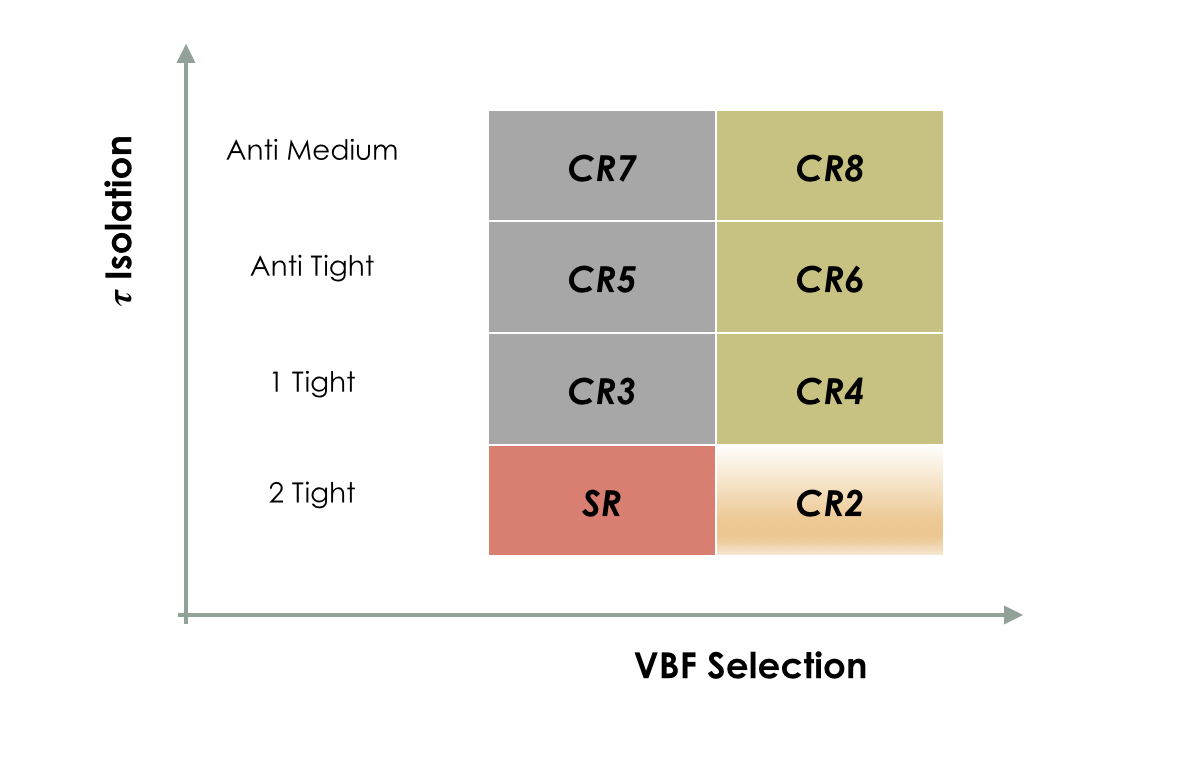
\includegraphics[width=0.75\textwidth]{PLOTS/diTauHadLSotherPlots/controlregions.png}
		%TODO i find the direction of the axes confusing: from left to right I would expect increasing VBF, from bottom to top I expect increasing levels of isolation while it’s the opposite in your drawing
	\end{tabular}
	\caption{Definition of Signal and Control Regions using different $\hadtau$ isolation criteria and VBF selection.}
	\label{fig:crs}
\end{figure}

\begin{equation}
\epsilon^{QCD}_{VBF} = \frac {N^{DATA}_{VBF CR} - N^{\overline{QCD} BG}_{VBFCR}}{\left( N^{DATA}_{VBFCR} - N^{\overline{QCD} BG}_{VBFCR} \right) + \left( N^{DATA}_{\overline{VBF}CR} - N^{\overline{QCD} BG}_{\overline{VBF}CR} \right) }
\label{eq:vbfeff}
\end{equation}

where $N^{DATA}_{VBF CR}$ is the number of the events in data for a given $ \tau $ isolation region and VBF region, $N^{\overline{QCD} BG}_{VBFCR}$ is the number of all non-QCD MC events for a given $ \tau $ isolation region and VBF region, $N^{DATA}_{\overline{VBF}CR}$ is the number of events in data in the same isolation Control Region but inverted VBF region and$N^{\overline{QCD} BG}_{\overline{VBF}CR}$ is the number of all non-QCD MC events for a given $ \tau $ isolation region but inverted VBF region.

%TODO here the reader needs to be referred to the table

%TODO one topic per paragraph

Using the events coming from the defined control regions as input for equations \ref{eq:qcdbgpred} and \ref{eq:vbfeff} gives the possibility to determine three different predictions for the QCD background contribution, one for each pair of tau isolation control regions below the two-tight isolation region. The estimation of the QCD contamination, in the signal region, as shown on Equation \ref{eq:qcdbgpred}, has three sources of systematics. The first source comes from the generated Monte Carlo samples used in the analysis. The two remaining ones comes from the assumptions about the stability of the $\epsilon^{QCD}_{VBF}$, made when defining the data-driven method, one in regard to a loosening of the tau-identification and the other in regard to a loosening of the \met cut, since the $\epsilon^{QCD}_{VBF}$ is calculated in CRs where no \met cut is applied.

Details and results on the validation process done for all the statements is given in Section \ref{QCD_bg_pred_validation}.


%TODO explain what should we learn from figure 6.12 and 6.13

The signal and control regions are define under the assumption of central selection being orthogonal to VBF selection. Figure \ref{fig:LS_mjjshapestab_vs_tauiso_data} and \ref{fig:LS_mjjshapestab_vs_tauiso_mc} shows the results of the stability study of $M_{jj}$ shape distribution among different $\tau$ isolation sidebands for Data and MC. Further studies are shown in Section \ref{dihad:tab:stability}.

\begin{figure}[tbh!]
	\centering
	\begin{tabular}{cc}
		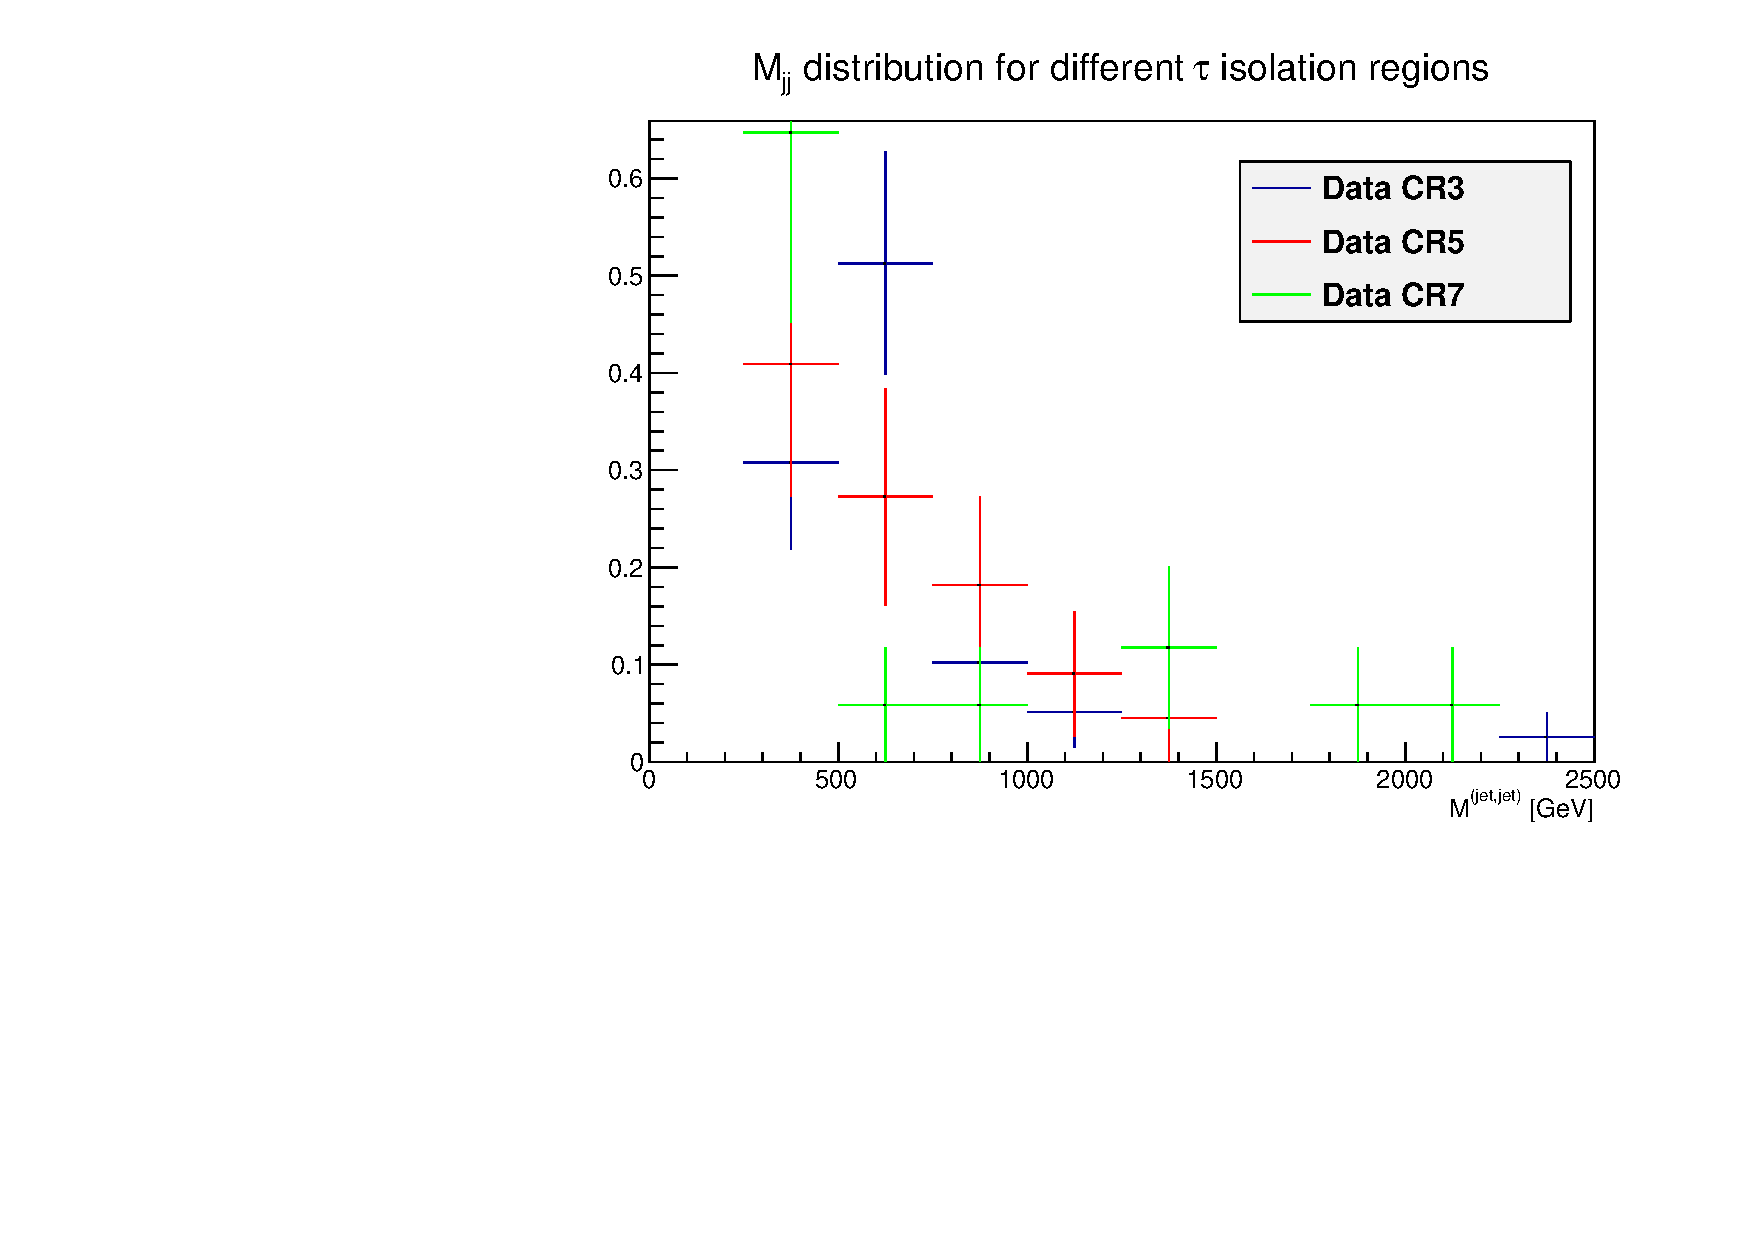
\includegraphics[width=0.75\textwidth]{PLOTS/diTauHadLSotherPlots/LS_mjjshapestab_vs_tauiso_data.pdf}
	\end{tabular}
	\caption{$M_{jj}$ shape comparisons among different $\tau$ isolation sidebands for Data (CR3, CR5, CR7)}
	\label{fig:LS_mjjshapestab_vs_tauiso_data}
\end{figure}

\begin{figure}[tbh!]
	\centering
	\begin{tabular}{cc}
		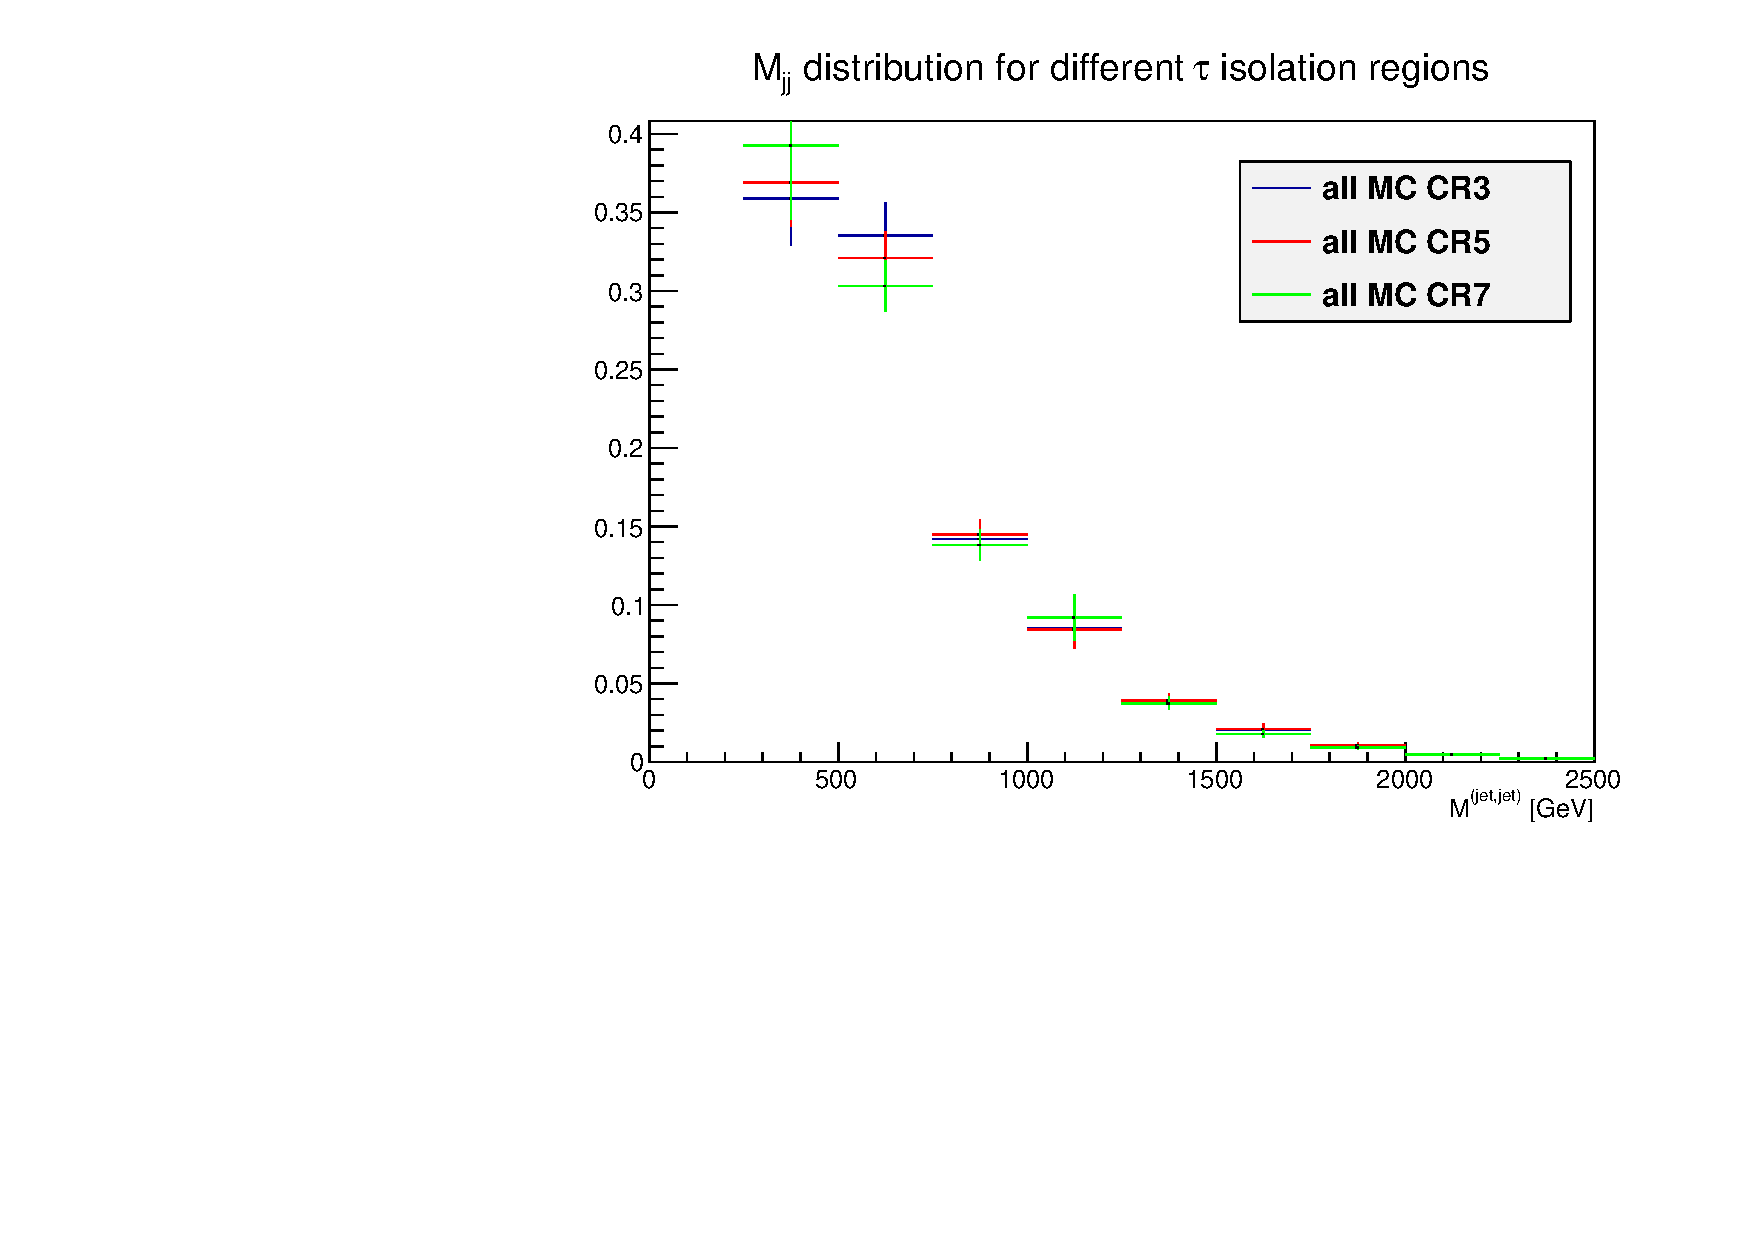
\includegraphics[width=0.75\textwidth]{PLOTS/diTauHadLSotherPlots/LS_mjjshapestab_vs_tauiso_mc.pdf}
	\end{tabular}
	\caption{$M_{jj}$ shape comparisons among different $\tau$ isolation sidebands for all MC contributions (CR3, CR5, CR7)}
	\label{fig:LS_mjjshapestab_vs_tauiso_mc}
\end{figure}

%TODO keep the SR column for the result section (where you fill in data) if you use a sideways table, scientific notation and proper rounding you’ll probably get tables 6.1 - 6.3 in one table

\begin{table}[ht]
	\centering{
		%   \tabcolsep=0.05cm
		\begin{tabular}{| l | c | c | c |}
			\hline\hline
			Sample     &Events (SR)   &Events (CR2)     &Events (CR3)       \\ [0.5ex] \hline
			Data &$ - $    &$ 109$    &$ 39$     \\
			Drell-Yan &$ 0.037\pm0.015$    &$ 1.3\pm1$    &$ 0.042\pm0.0077$     \\
			VV &$ 0.11\pm0.065$    &$ 0.7\pm0.09$    &$ 0.035\pm0.017$    \\
			W+Jets &$ 0.53\pm0.04$    &$ 6.6\pm0.17$    &$ 0.83\pm0.055$    \\
			Single t &$ 0.036\pm0.0066$    &$ 0.25\pm0.017$    &$ 0.057\pm0.008$   \\
			\ttbar &$ 0.11\pm0.012$    &$ 1.4\pm0.051$    &$ 0.19\pm0.013$   \\
			Higgs &$ 0.0005\pm7.2e^{-05}$    &$ 0.012\pm0.0048$    &$ 0.0029\pm0.0023$   \\
			QCD &$ 8.6\pm0.61$    &$ 54\pm1.2$    &$ 47\pm1.9$   \\
			\hline
			Total nonQCD MC &$ 0.83\pm0.079$    &$ 10\pm1$    &$ 1.2\pm0.06$   \\
			\hline\hline
		\end{tabular}
	}
	\caption{Number on events in SR, CR2, CR3 for data and all MC samples used for the estimation of $N^{QCD}_{SR}$}
	\label{table:CReventcount1} % is used to refer this table in the text
\end{table}

\begin{table}[ht]
	\centering{
		%   \tabcolsep=0.05cm
		\begin{tabular}{| l | c | c | c |}
			\hline\hline
			Sample   &Events (CR4)  &Events (CR5)     &Events (CR6)    \\ [0.5ex] \hline
			Data    &$ 737$  &$ 22$    &$ 312$      \\
			Drell-Yan    &$ 0.65\pm0.045$  &$ 0.002\pm0.00076$    &$ 0.029\pm0.0037$    \\
			VV   &$ 0.6\pm0.1$   &$ 0.0031\pm0.001$    &$ 0.045\pm0.015$   \\
			W+Jets    &$ 10\pm0.2$  &$ 0.081\pm0.0096$    &$ 0.89\pm0.034$      \\
			Single t   &$ 0.47\pm0.02$   &$ 0.011\pm0.00076$    &$ 0.1\pm0.0028$      \\
			\ttbar  &$ 2.5\pm0.059$   &$ 0.04\pm0.0024$    &$ 0.52\pm0.0095$      \\
			Higgs  &$ 0.012\pm0.0044$   &$ 2.7e-05\pm1.1e-05$    &$ 0.00018\pm2.2e-05$    \\
			QCD  &$ 3.4e+02\pm4$  &$ 19\pm0.68$    &$ 1.4e+02\pm1.6$    \\
			\hline
			Total nonQCD MC  &$ 15\pm0.24$ &$ 0.14\pm0.01$    &$ 1.6\pm0.038$    \\
			\hline\hline
		\end{tabular}
	}
	\caption{Number on events in CR4, CR5, CR6 for data and all MC samples used for the estimation of $N^{QCD}_{SR}$}
	\label{table:CReventcount2} % is used to refer this table in the text
\end{table} 

\begin{table}[ht]
	\centering{
		%   \tabcolsep=0.05cm
		\begin{tabular}{| l | c | c |}
			\hline\hline
			Sample      &Events (CR7)     &Events (CR8)  \\ [0.5ex] \hline
			Data     &$ 17$    &$ 184 $  \\
			Drell-Yan    &$ 0.0012\pm0.00057$    &$ 0.013\pm0.0021 $  \\
			VV   &$ 0.0011\pm0.00014$    &$ 0.033\pm0.016 $  \\
			W+Jets    &$ 0.036\pm0.0051$    &$ 0.35\pm0.015 $  \\
			Single t   &$ 0.0061\pm0.00045$    &$ 0.058\pm0.00087 $  \\
			\ttbar  &$ 0.022\pm0.00079$    &$ 0.32\pm0.0054 $  \\
			Higgs  &$ 4.9e-06\pm2.3e-06$    &$ 5.7e-05\pm1e-05 $  \\
			QCD  &$ 15\pm0.81$    &$ 1.1e+02\pm1.7 $  \\
			\hline
			Total nonQCD MC  &$ 0.067\pm0.0053$    &$ 0.77\pm0.023 $  \\
			\hline\hline
		\end{tabular}
	}
	\caption{Number on events in CR7 and CR8 for data and all MC samples used for the estimation of $N^{QCD}_{SR}$}
	\label{table:CReventcount3} % is used to refer this table in the text
\end{table} 

\begin{table}[ht]
	\centering{
		\tabcolsep=0.05cm
		\begin{tabular}{| l | c | c | c |}
			\hline\hline
			Variable     &One Tight region     &Anti-Tight region     &Anti-Medium  \\ [0.5ex] \hline
			$\epsilon^{QCD}_{VBF}$    &$ 0.05\pm0.008 $  &$ 0.066\pm0.014 $  &$ 0.085\pm0.02 $ \\
			$N^{QCD}_{SR}$    &$ 5.2\pm1 $  &$ 6.9\pm1.7 $  &$ 9.1\pm2.5 $ \\
			\hline\hline
		\end{tabular}
	}
	\caption{ Values for $\epsilon^{QCD}_{VBF}$ and $N^{QCD}_{SR}$ for different $ \tau $ isolation regions.}
	\label{table:VBFeffBKGprediction} % is used to refer this table in the text
\end{table}

%TODO replace “systematics” with amore precise description, and motivate the method.

Systematics for the simulation are estimated by scaling non-QCD contributions by $\pm50~\%$. A systematic error on $\epsilon^{QCD}_{VBF}$ is assigned by using the maximal variation among all $\epsilon^{QCD}_{VBF}$ measurements in different $\tau$ isolation regions with respect to its weighted mean. Similar procedure is done for the assignation of the $\epsilon^{QCD}_{VBF}$ coming from \met cut stability. All the statistical uncertainties are propagated accordingly. Tables \ref{table:CReventcount1} , \ref{table:CReventcount2} and \ref{table:CReventcount3} show the event counting for all the control regions previously defined for data and all MC samples. All the numbers except the ones coming from the QCD sample are used as input for the QCD background estimation method. For each of the 3 different $\tau$ isolation regions out of the signal region (1T, AT, AM) an independent measurements of $\epsilon^{QCD}_{VBF}$  and prediction for $N^{QCD}_{SR}$ is made. Due to low statistics in the $\tau$ isolation sidebands the final results will include uncertainties coming from the $\epsilon^{QCD}_{VBF}$ stabilities studies on MC shown in section \ref{subsec:stability}.

\clearpage

\section{Data Driven method validation}
\label{QCD_bg_pred_validation}

While a data-driven approach with an ABCD method in data is utilizable in order to get a prediction for the number of background events expected in the signal region, there are two advantages of a simulation-based approach. On the one hand, one can ascertain that the control regions contain only QCD. On the other hand, one can provide a closure test for the data-driven prediction, especially regarding the universality of the VBF efficiency with respect to a loosening of the τh isolation or a relaxation of the \met requirement, as stated in Sec. ???.

In order to achieve the goal to ensure QCD purity in the control regions, a straightforward use of the simulation is not possible, due to the low probability of jets to fake \hadtau with any identification (ID), be it tight (T), medium (M), or loose (L). These low rates decrease the number of simulated events with two reconstructed \hadtau leptons passing all selection requirements below any reasonable amount for direct usage. What can be done, is to estimate the probability of one jet to be misidentified as a \hadtau lepton (O ≈ 1 ) of a given exclusive isolation (see Tab. ??? in Sec. ??? for definitions), 100 instead. Using all simulated events with four or more jets, one can determine the chance of each such event to be reconstructed as one event with two \hadtau leptons and at least two jets, translating two jet objects to become \hadtau objects (see Sec. ???). This way, a meaningful study of systematic uncertainties of the background estimation method on data becomes possible and the prerequisite assumptions of QCD purity and stability of the VBF efficiency with respect to \hadtaufake isolation can be tested. Finally, the results of the application of this method and thereby estimated systematic uncertainties will be shown (see Sec. ???). As well, possible future data-driven improvements for this method will be outlined (see Sec. ???).

\subsection*{Redefining jets as \hadtau}

\subsection*{Selection acceptance correction}

\subsection*{parametrization for fake probabilities}

\subsection*{Trigger acceptance correction}

\subsection*{Fixation of fake \hadtau mass}

\subsection{$\epsilon^{VBF}$-stability with regard to $\tau_{h}$-isolation and $E_{T}^{miss}$-cuts}\label{dihad:subsec:stability}
To test the stability and estimate the systematics, we determine on the diced MC all possible efficiencies of $\epsilon^{VBF}$ in all even and odd control region pairs for a range of $E_{T}^{miss}$-cuts in table \ref{dihad:tab:stability}.
\begin{table}[!h]
	\centering
	\begin{tabular}{|c||c|c|c|}
		\hline
		region     & $\epsilon^{VBF}(E_{T}^{miss}\geq0)$ [$\%$]& $\epsilon^{VBF}(E_{T}^{miss}\geq10)$ [$\%$]& $\epsilon^{VBF}(E_{T}^{miss}\geq20)$ [$\%$]\\ \hline \hline
		LS SR/CR2  & $12.78\pm0.53$ & $12.91\pm0.58$ & $13.06\pm0.67$ \\ \hline
		LS CR3/CR4 & $12.20\pm0.43$ & $12.48\pm0.47$ & $12.46\pm0.53$ \\ \hline
		LS CR5/CR6 & $11.61\pm0.41$ & $11.93\pm0.45$ & $11.91\pm0.50$ \\ \hline
		LS CR7/CR8 & $12.10\pm0.60$ & $12.44\pm0.66$ & $12.75\pm0.83$ \\ \hline \hline
		OS SR/CR2  & $11.46\pm0.72$ & $11.74\pm0.80$ & $12.23\pm1.04$ \\ \hline
		OS CR3/CR4 & $10.62\pm0.31$ & $10.66\pm0.33$ & $10.85\pm0.36$ \\ \hline
		OS CR5/CR6 & $10.98\pm0.48$ & $11.09\pm0.52$ & $11.59\pm0.67$ \\ \hline
		OS CR7/CR8 & $10.67\pm0.36$ & $10.61\pm0.37$ & $11.12\pm0.47$ \\ \hline \hline
		WAM        & $11.33\pm0.15$ & $11.43\pm0.16$ & $11.66\pm0.19$ \\ \hline
		\hline
		\hline
		region     & $\epsilon^{VBF}(E_{T}^{miss}\geq30)$ [$\%$]& $\epsilon^{VBF}(E_{T}^{miss}\geq40)$ [$\%$]& $\epsilon^{VBF}(E_{T}^{miss}\geq50)$ [$\%$]\\ \hline \hline
		LS SR/CR2  & $13.76\pm0.89$ & $14.99\pm1.49$ & $18.09\pm2.93$ \\ \hline
		LS CR3/CR4 & $13.18\pm0.68$ & $14.54\pm1.11$ & $16.58\pm2.08$ \\ \hline
		LS CR5/CR6 & $12.20\pm0.56$ & $13.06\pm0.84$ & $13.34\pm1.12$ \\ \hline
		LS CR7/CR8 & $14.05\pm1.25$ & $15.93\pm2.19$ & $19.26\pm4.14$ \\ \hline \hline
		OS SR/CR2  & $13.14\pm1.58$ & $16.04\pm2.98$ & $21.23\pm6.13$ \\ \hline
		OS CR3/CR4 & $11.08\pm0.41$ & $12.61\pm0.69$ & $14.45\pm1.23$ \\ \hline
		OS CR5/CR6 & $12.19\pm0.95$ & $14.38\pm1.70$ & $18.22\pm3.42$ \\ \hline
		OS CR7/CR8 & $11.37\pm0.54$ & $13.01\pm0.90$ & $14.76\pm1.62$ \\ \hline \hline
		WAM        & $11.98\pm0.23$ & $13.43\pm0.39$ & $14.85\pm0.65$ \\ \hline
	\end{tabular}
	\caption{Stability of epsilonVBF in regard to $E_{T}^{miss}$, sign and $\tau_{h}$-isolation. LS and OS regions are slightly correlated. Here, events can be the same, but the chosen jets to fake $\tau_{h}$ must differ. For efficiencies of one sign, efficiencies are expected to be highly correlated. This is not accounted for in the weighted arithmetic mean (WAM) values shown.}
	\label{dihad:tab:stability}
\end{table}
We do observe a quadratic dependence on $E_{T}^{miss}$, as seen in fig. \ref{dihad:fig:Stability}.

\begin{figure}[!h]
	\centering
	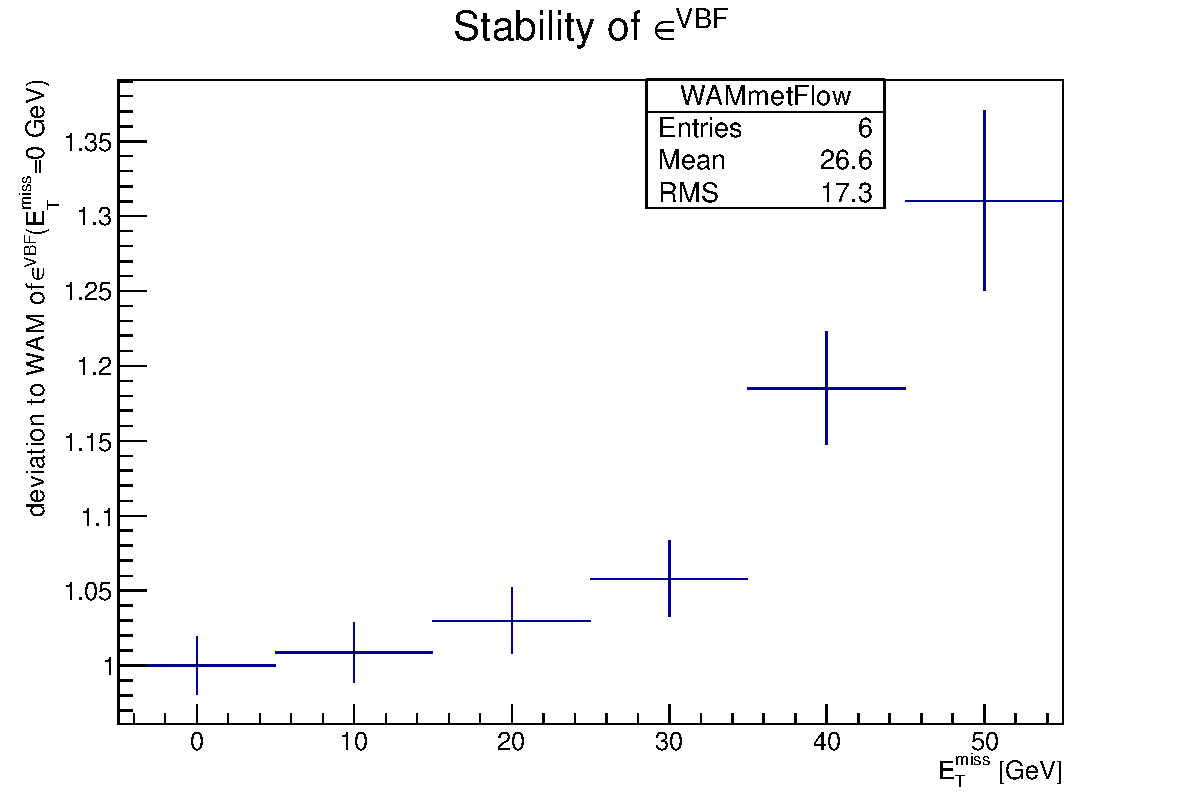
\includegraphics[width=0.5\textwidth]{PLOTS/diTauHadLSQCDPlots/stability/Stability.pdf}
	\caption{\label{dihad:fig:Stability}Deviation of the weighted arithmetic mean (WAM) of the VBF efficiency of all (LS and OS) control region ratios with respect to $E_{T}^{miss}$. We observe a quadratic dependence of small size at the cut-value of 30 GeV we use in this analysis.}
\end{figure}

We derive two systematic errors out of this:
\begin{enumerate}
	\item Stability of $\epsilon^{VBF}$ regarding $\tau_{h}$-isolation: Maximum relative difference to weighted arithmetic mean at $E_{T}^{miss}\geq30$. Amounts to $+17.26\%$ and $-7.58\%$.
	\item Stability of $\epsilon^{VBF}$ regarding $E_{T}^{miss}$-cut: Relative difference to $\epsilon^{VBF}$ within uncertainties of weighted arithmetic
	mean at no cut on $E_{T}^{miss}$ as seen in fig. \ref{dihad:fig:Stability}. Amounts to $+8.30\%$ on the upper edge and $+3.26\%$ on the lower edge.
\end{enumerate}

\clearpage




\cleardoublepage

\chapter{Results}
\label{sec:results}
\section{Results}
\label{section:results}

As shown in section \ref{sec:bgestimation} $\epsilon^{QCD}_{VBF}$ is calculated for OS ans LS. Uncertainties coming from the stability studies on MC shown in section \ref{dihad:subsec:stability} has been taken into account. The weighted average mean coming from the two different measurements gives the following final result:

\begin{equation}
\epsilon^{QCD}_{VBF} = 0.067\pm0.0046(stat.)^{-0.00038(MC)+0.0117(\tau iso)+0.0056(MET)}_{+0.00022(MC)-0.0051(\tau iso)+0.0022(MET)}
\label{eq:vbfefflsresult}
\end{equation}

Using the following efficiency in Equation \ref{eq:qcdbgpred} gives the final QCD background prediction in signal region:

\begin{equation}
N^{QCD}_{SR} = 7.14\pm0.92(stat.)^{-0.42(MC)+1.34(\tau iso)+0.64(MET)}_{+0.35(MC)-0.58(\tau iso)+0.25(MET)}
\label{eq:QCDbgpredresult}
\end{equation}

This final estimate is corrected for the MET bias by taking the central value of the  bias as a correction and 
the uncertainty of the central value as a symmetric uncertainty. The result of this correction is shown in Eq.
\ref{dihad:eq:QCDbgpredCorrectResult}

\begin{equation}
N^{QCD}_{SR} = 7.59\pm0.92(stat.)^{-0.42(MC)+1.34(\tau iso)+0.20(MET)}_{+0.35(MC)-0.58(\tau iso)-0.20(MET)}
\label{dihad:eq:QCDbgpredCorrectResult}
\end{equation}

\clearpage
\section{Final Yields for LS channel}

The LS signal region consist of events satisfying the criteria shown in section \ref{sec:eventselection} with the di-$\tau$ charge requirement. As described in section \ref{dihad:subsubsec:eventweight} all the backgrounds have been reweighted with $\tau_{h}^{fake}$ reweighting method. Table \ref{table:SReventcount} shows the contributions in the signal region from all MC samples and data.  QCD is the dominant background and its prediction shown in section \ref{section:results} is compatible with the number in table \ref{table:SReventcount}. Figure \ref{fig:LS_SR_h_met_dijetinvariantmass_log}(a) shows the expected and observed signal rate in bins of \met. Figure \ref{fig:LS_SR_h_met_dijetinvariantmass_log}(b) shows the expected and observed signal rate in bins of $M_{jj}$. We observe a good agreement in all the distributions range between observed data and the SM prediction. Additional distributions for signal region have been included in the Appendix.

   \begin{table}[ht]
     \centering{
     
  %   \tabcolsep=0.05cm
      \begin{tabular}{| l | c |}
         \hline\hline
         Sample     &Events (SR)      \\ [0.5ex] \hline
Data &$ 9 $     \\
Drell-Yan &$ 0.037\pm0.015$      \\
VV &$ 0.11\pm0.065$     \\
W+Jets &$ 0.53\pm0.04$        \\
Single t &$ 0.036\pm0.0066$    \\
TTbar &$ 0.11\pm0.012$    \\
Higgs &$ 0.0005\pm7.2e-05$     \\
QCD Prediction &$ 7.59\pm0.92(stat.)^{+1.38}_{-0.72}(syst.)$    \\
\hline
Total nonQCD MC &$ 0.83\pm0.079(stat.)\pm0.41(syst.)$    \\
         \hline\hline
       \end{tabular}
     }
     \caption{\label{table:SReventcount}Number on events in SR data and all MC samples. The QCD prediction has been corrected for the unidirectional MET-bias described in section \ref{dihad:subsec:stability} for the combination of the systematic errors.}
      % is used to refer this table in the text
   \end{table}
   
       \begin{figure}[tbh!]
           \centering
           \begin{tabular}{cc}
             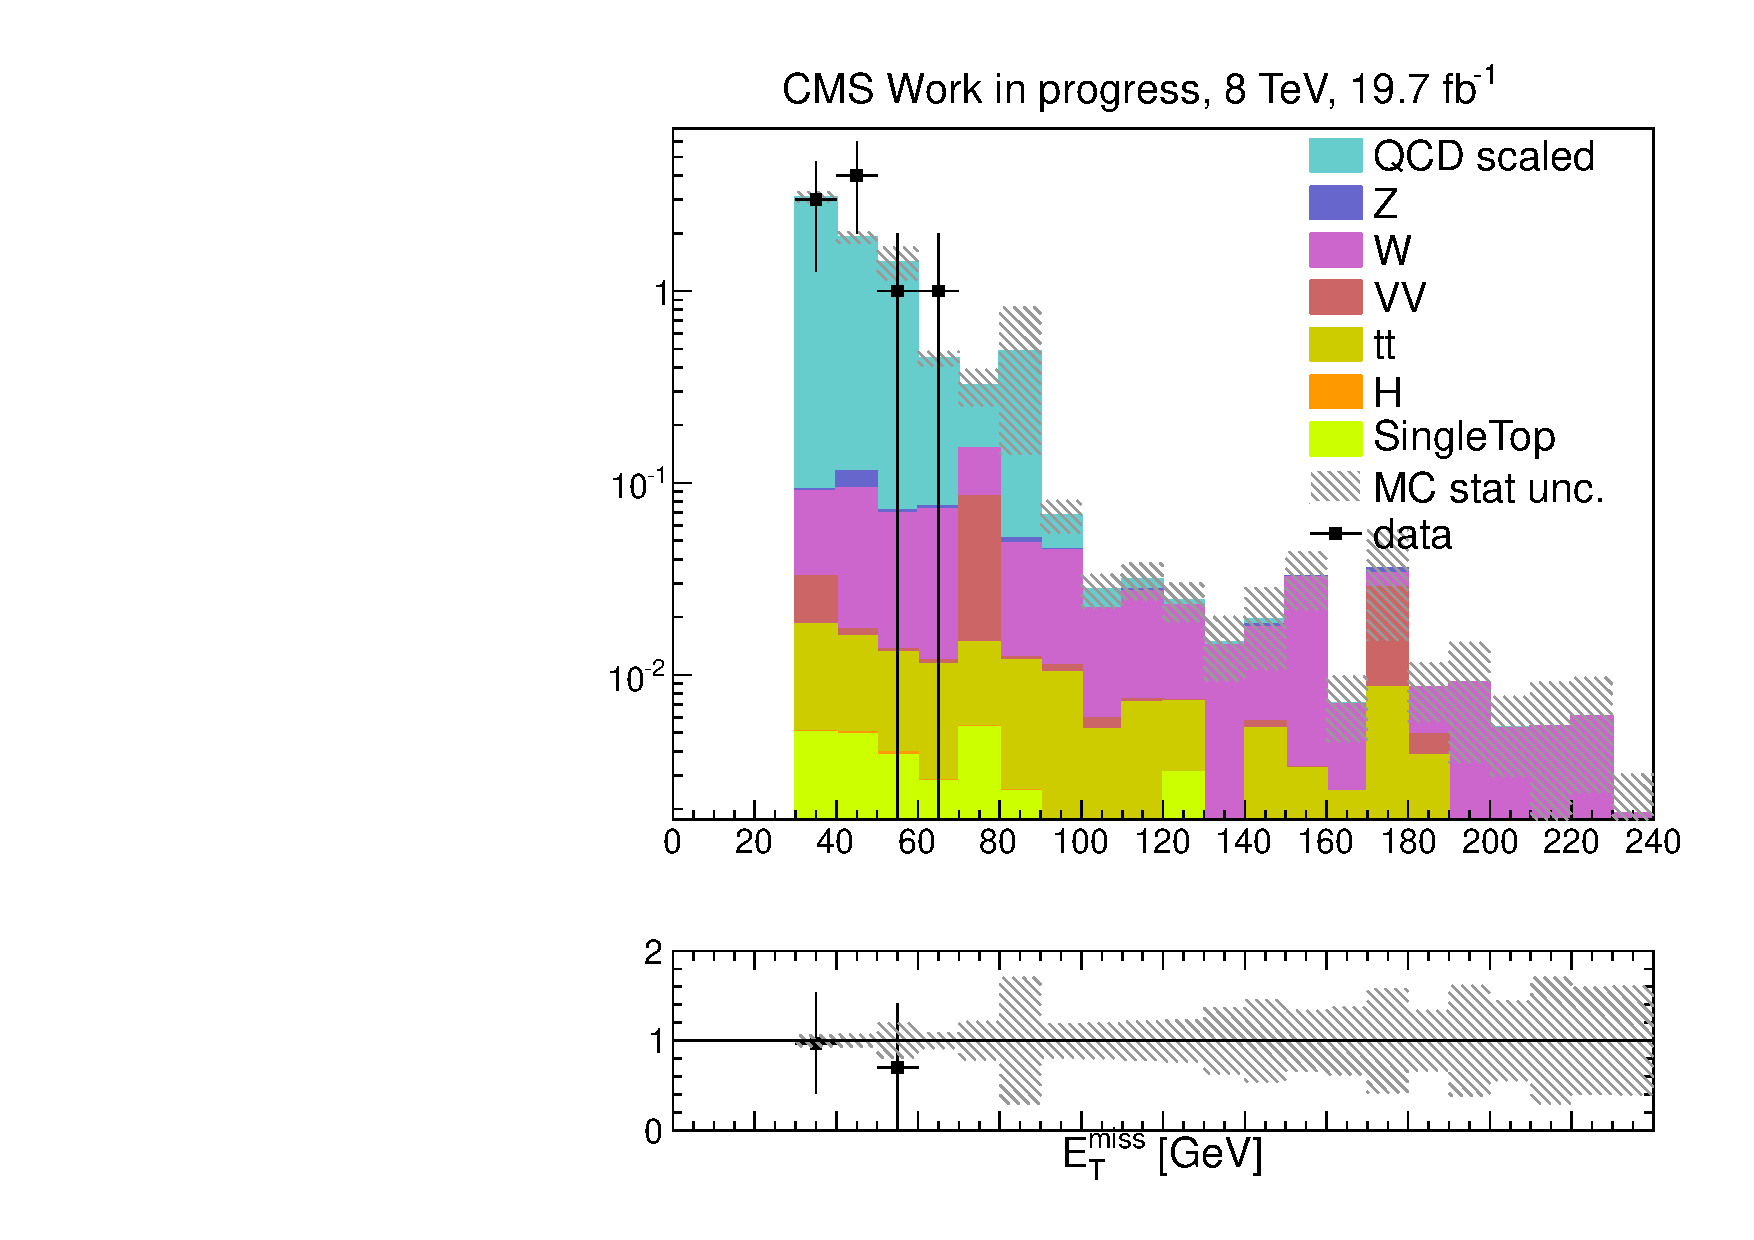
\includegraphics[width=0.40\textwidth]{PLOTS/diTauHadLSQCDPlots/UnblindedUpdate/LS_SR/LS_SignalRegion/h_met_log.pdf}
             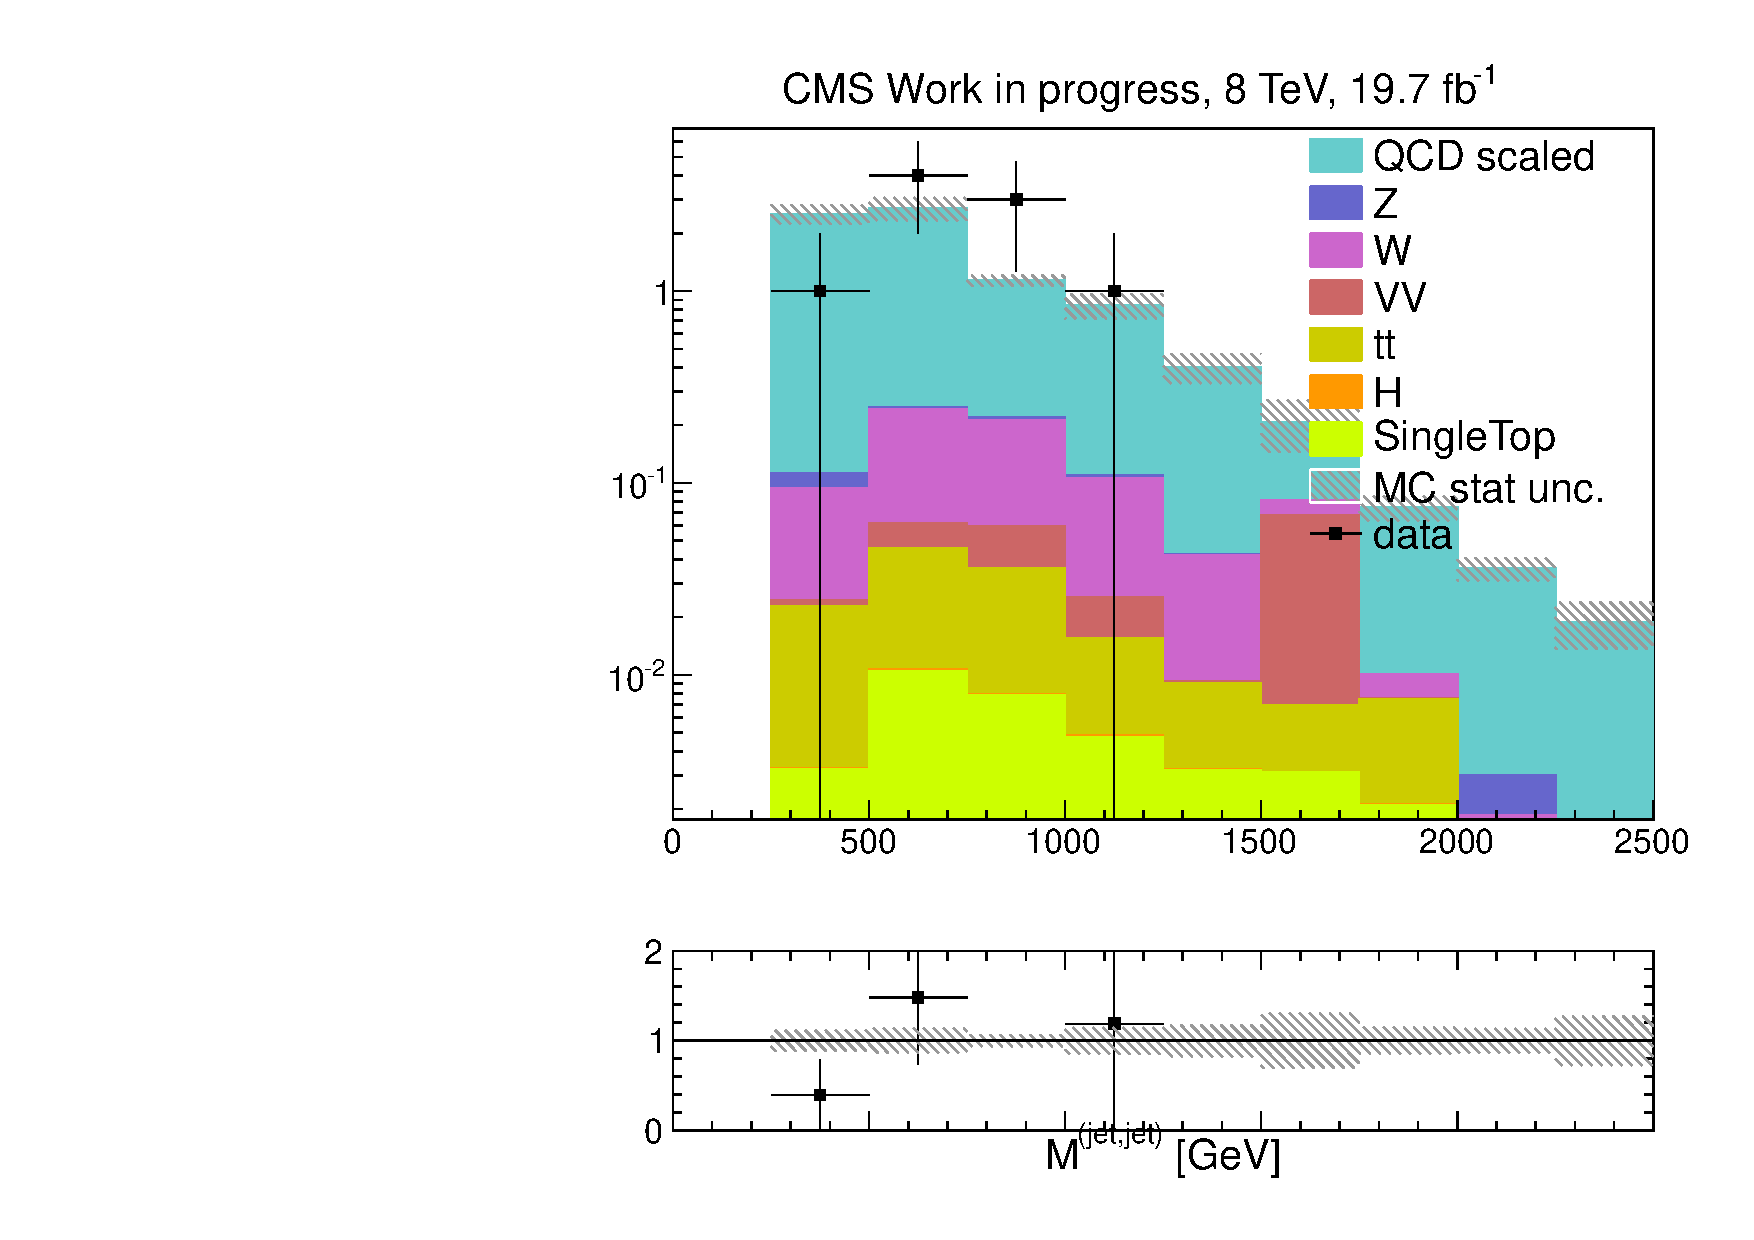
\includegraphics[width=0.40\textwidth]{PLOTS/diTauHadLSQCDPlots/UnblindedUpdate/LS_SR/LS_SignalRegion/h_dijetinvariantmass_log.pdf}
           \end{tabular}
           \caption{(a)\met and (b)$M_{jj}$ distributions in signal region for Data and all MC samples}
           \label{fig:LS_SR_h_met_dijetinvariantmass_log}
         \end{figure}

\clearpage 
\section{Systematics}
\label{sec:systematics}

The following systematics have been considered:

\begin{itemize}
  \item \textbf{Parton Distribution Functions (PDF):} The systematic effect due to imprecise knowledge of the parton 
distribution functions is determined by comparing CTEQ6.6L \cite{Nadolsky:2008zw}, MSTW2008nnlo \cite{Martin:2009iq}, and NNPDF20 PDF \cite{Ubiali:2008uk} with the default PDF and variations within the family of parametrization. The maximal deviation from the central value is used the overall systematic due to PDFs. We obtain a value of 16\% on the cross section uncertainty and 23\% on the signal acceptance.

  \item \textbf{Initial State Radiation (ISR) and Final State Radiation (FSR):} The systematic effect due to imprecise modeling of initial and final state radiation is determined by re-weighting events to account for effects such as missing a terms in the soft-collinear approach \cite{softCollinear} and missing NLO terms in the parton shower approach \cite{partonShower}. We obtain uncertainties of 0.9\% and 1.2\% for ISR and FSR respectively.

  \item \textbf{Luminosity:} We consider a 2.6\% uncertainty on the measured luminosity \cite{CMS:2012rua}.
  
  \item \textbf{Trigger, Reconstruction, and Selection:}  An overall uncertainty is applied for the trigger uncertainties determined on the
  correction factors described in AN-12-321 and which are measured using tag-and-probe methods. We consider 6.8\% uncertainty per hadronic tau leg \cite{CMS:2011msa}. Scale factors for $\tau_{h}$ identification are taken from the tau POG and obtained using a fit of data in a Z$\to\tau\tau$ enhanced region and fixing the cross section to that measured using ee/$\mu\mu$. We consider a 100\% correlation among the 2 tau legs, therefore we consider 13.6\% uncertainty on the signal acceptance.

  \item \textbf{$b$-Tagging Efficiency:} We consider a 30\% uncertainty on the mis-tag rate as measured by the b-tagging POG \cite{CMS:2011cra}. For the case of our signal, the systematic uncertainty on the requirement of 0 jets mis-tagged as b-jets is determined by propagating the 30\% uncertainty on the mis-tag rate through the following equation (which represents the signal efficiency for requiring 0 jets mis-tagged as b-Jets):

\begin{equation}\label{eq:nttbar}
  \epsilon^{\textrm{NBtag} < 1} = 1 - \sum_{n=1} P(n) \cdot \sum_{m=1}^{n} C(n,m) \cdot f^{m} \cdot (1-f)^{n-m}
\end{equation}

where $P(n)$ is the probability to obtain $n$ additional jets (non-tau and non-lepton) in the event, $C(n,m)$ the 
combinatorial of $n$ $choose$ $m$, and $f$ the mis-tag rate. The probability to 
obtain at least one additional jet in the event is much less than 1\%. Therefore, based on the above equation, the 
mis-tag rate and uncertainty, and the probability to obtain at least one additional jet we calculate a negligible 
systematic effect on our signal due to the mis-tag rate.

  \item \textbf{Tau Energy Scale:} We consider the effect of the 3\% tau energy scale uncertainty measured by the tau 
POG on the signal acceptance. The tau 4-momentum is scaled by a factor of $k=1.03$ ($p_{smeared} = k \cdot 
p_{default}$) and variables are recalculated using $p_{smeared}$. We find that by using $p_{smeared}$ calculated with 
a factor of $k=\pm 1.03$, the signal acceptance fluctuates by 4\%. Therefore, we assign a 4\% systematic on the signal 
acceptance due to tau energy scale.
  \item \textbf{Jet Energy Scale:}  The uncertainty on jet energy correction (JEC) is the result of a factorized approach on $Anti­-k_{t}$ jets with $R=0.5$ clustered from Particle Flow (PF) candidates. For MC samples JEC is divided in different steps that take into account several levels of correction. The fist step consist in a single level of corrections (L1) which estimates the $p_{t}$ offset in bins of $\eta$ and $N_{PV}$ for AK5PF jets. The second step, known as MC­ - Truth Corrections, consists in two level of corrections (L2 and L3) converging into an $\eta$ , $p_{t}$ ­dependent scaling factor fully derived from MC after applying L1­ corrections. The last step takes into account an L5 correction and uncertainties for individual flavors and predefined mixtures inside the reconstructed jets. We assign a 2\% systematic on the signal acceptance due to jet energy scale.
  \item \textbf{Jet Energy Resolution:}  The measured jet transverse momentum is not necessarily equal to the energy of the original particle due to e.g. a limited detector resolution. This effect is quantified by the jet transverse momentum response R which is defined as $R = p_{T} / p_{T}^{particle}$  where $p_{T}$ denotes the transverse momentum of the jet measured at detector level and $p_{T}^{particle}$ is the transverse momentum of the original particle-level jet. The average response $\langle R \rangle$ is referred to as jet energy scale and calibrated such that $\langle R \rangle = 1$ for fixed $p_{T}^{particle}$. The response usually depends on the jet momenta as well as on the pseudorapidity. This is expected since the quality of the jet measurement is directly related to the detector sub-components and the energy of the particles originating e.g. from the track-reconstruction efficiency or the individual amount of detector material. The core of the response is caused by the intrinsic resolution of the various sub-detector components and the precision of the jet clustering algorithms. The response tails are mainly caused by severe jet-mismeasurements. These can be e.g. detector effects like shower leakage or detector noise. Finally, the relative jet transverse momentum resolution is defined as the width of the response distribution corresponding to the gaussian part and hence is a function of $p_{T}$ and $\eta$ as well as the total response. One possibility to measure the resolution of the jet transverse momenta in data as well as in simulated events is to utilize the dijet asymmetry A. For events with at least two jets it is defined as:
  
  \begin{equation}
  A = \frac{p_{T,1} - p_{T,2}}{p_{T,1} + p_{T,2}}
  \end{equation}
  
  For a sufficient number of events the asymmetry is approximately normally distributed and its' stardard deviation is $\sigma_{A}$. In an ideal dijet topology the two jets are exactly balanced at particle level which leads to an important relation between the width of the asymmetry $\sigma_{A}$ and the jet-$p_{T}$ resolution $\sigma(p_{T})$:
  
  \begin{equation}
  \frac{\sigma(p_{T})}{\langle p_{T} \rangle} = \sqrt{2} \sigma_{A}
  \end{equation}
  
  Using the lastest JER uncertainty collection from \textit{Summer13\_V5\_DATA\_Uncertainty\-Sources\_AK5PFchs.txt} assign a 4\% systematic on the signal acceptance due to jet energy resolution. 

  \item \textbf{MET:} The uncertainty on MET for our signal process is driven by the jet energy 
scale (non-tau jets) (JES), light lepton energy/momentum scale (LES), and unclustered energy (UCE).
The systematic effect from MET due to TES, JES and LES is included in the JES,
TES, LES systematic uncertainties described above. We find that a 10\% uncertainty on the unclustered energy results
in at most a 0.5\% fluctuation on the signal acceptance.
\end{itemize}

\begin{table}[h]
	\centering{
		\begin{tabular}{| l | c | c |}
			\hline\hline
			Source            & Uncertainty & Signal \\
			\hline
			PDF               & ---                            & 23\%                       \\
			ISR/FSR           & ---                             & 1\%              \\
			Luminosity        & 2.6\%                           & 2.6\%                      \\
			Trigger, ID, Selection & 6.8\%                            & 16\%                       \\
			Tau Energy Scale  & --                             & 4\%                        \\
			b-Jet ID          & 30\%                            & 1\%                        \\
			JES               & 2\% - 10 \%                            & 2\%                      \\
			JER              & 5\% - 25 \%                            & 4\%                      \\
			MET               & 10\%                           & 0.5\%  \\
			\hline\hline                  
			\end{tabular}
	}
\caption{Summary of systematic uncertainties}
\label{table:Uncertainties}
\end{table}

Table \ref{table:Uncertainties} summarizes all the relevant uncertainties that has been considered. 

\clearpage

\section{Limits}

Similarly to what is done in AN-12-321 upper limits at $95\%$ on the cross sections as function of $m_{\tilde{\chi}_{2}^{0}}=m_{\tilde{\chi}_{1}^{\pm}}$ are set for LS and OS channel. The results are presented using models with a fixed mass for the LSP $m_{\tilde{\chi}_{1}^{0}} = 0 $ GeV, a $\tilde{\chi}_{1}^{\pm}$ mass between $100 \leq m_{\tilde{\chi}_{1}^{\pm}} \leq 300$ GeV and a $\tilde{\tau}$ mass of $m_{\tilde{\tau}} = 0.95 m_{\tilde{\chi}_{1}^{\pm}}$ .

\begin{figure}
  \begin{center}
    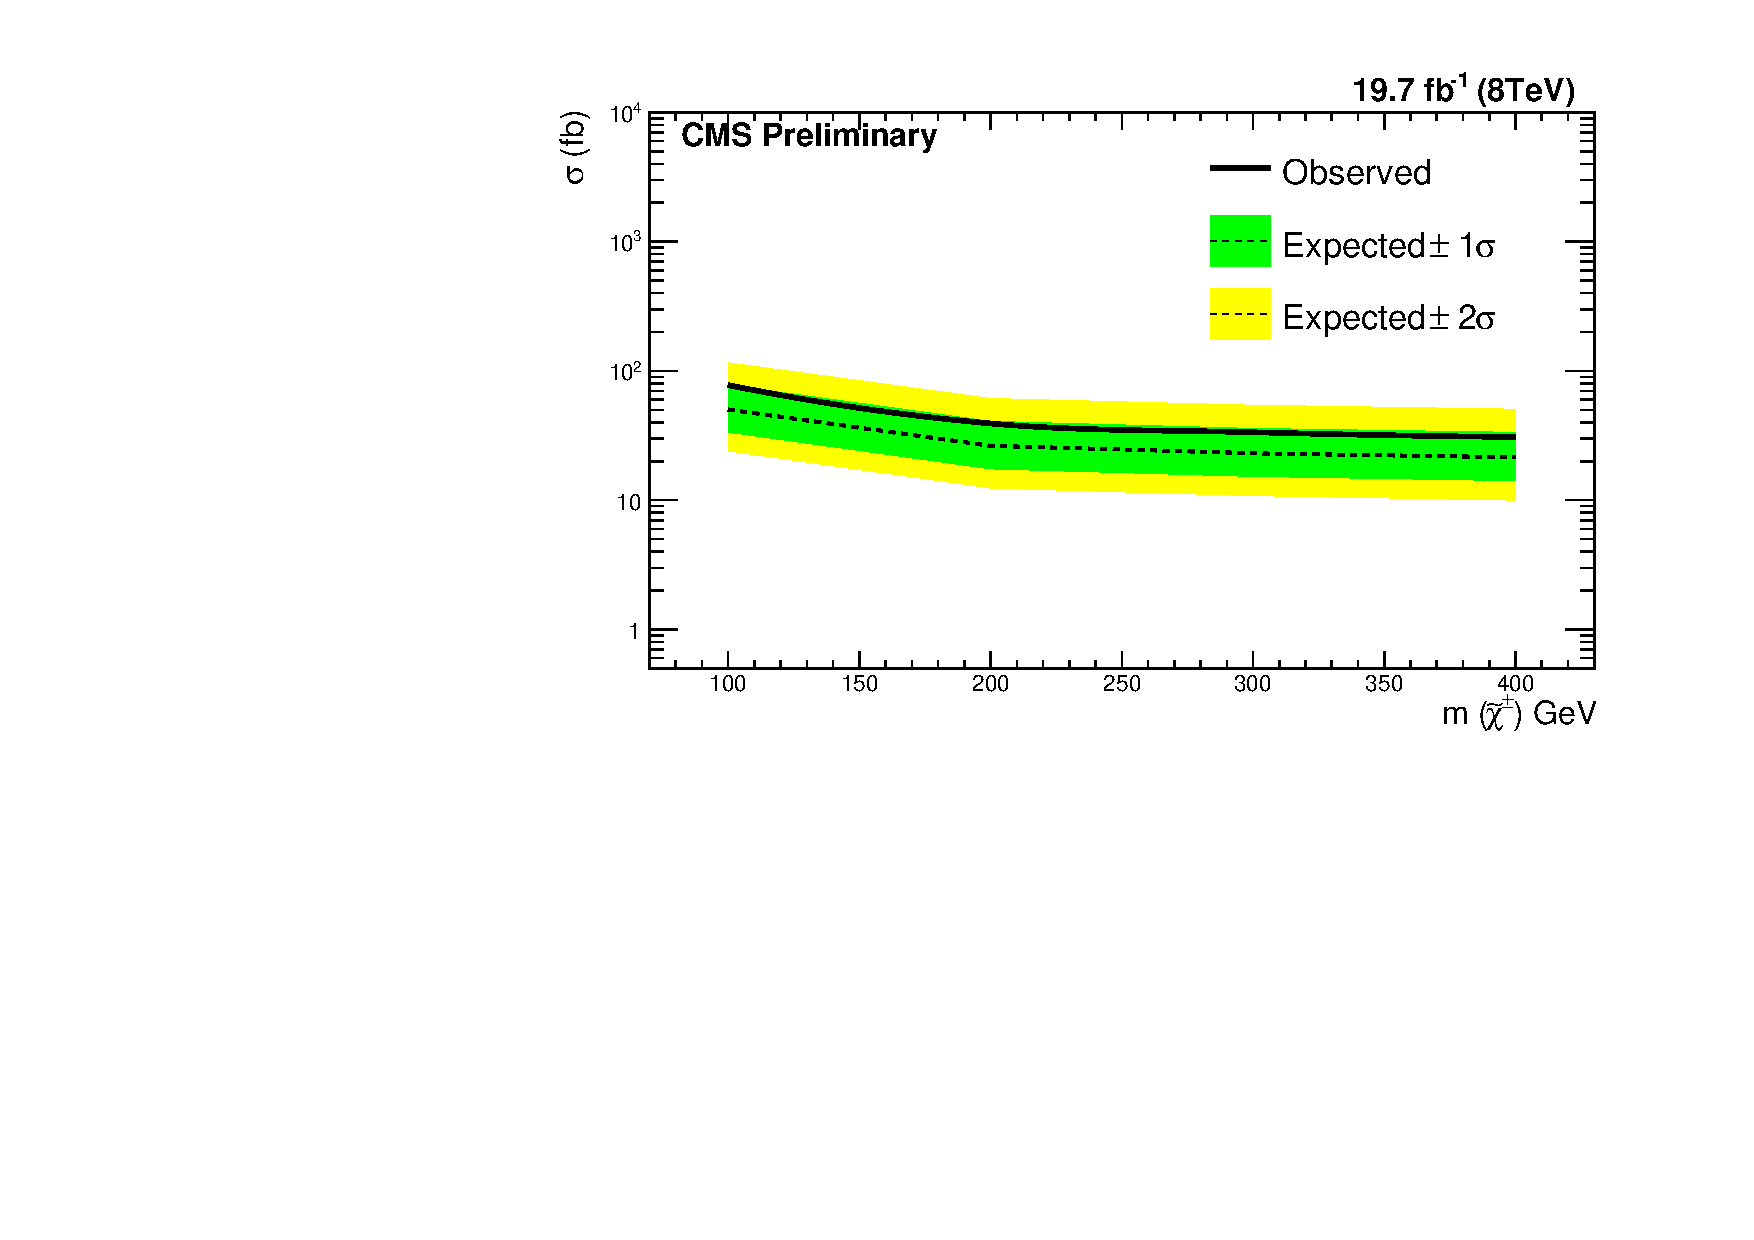
\includegraphics[angle=0,width=.48\textwidth, height=0.35\textheight]{PLOTS/Limit_VBF_diTau_OS.pdf}
    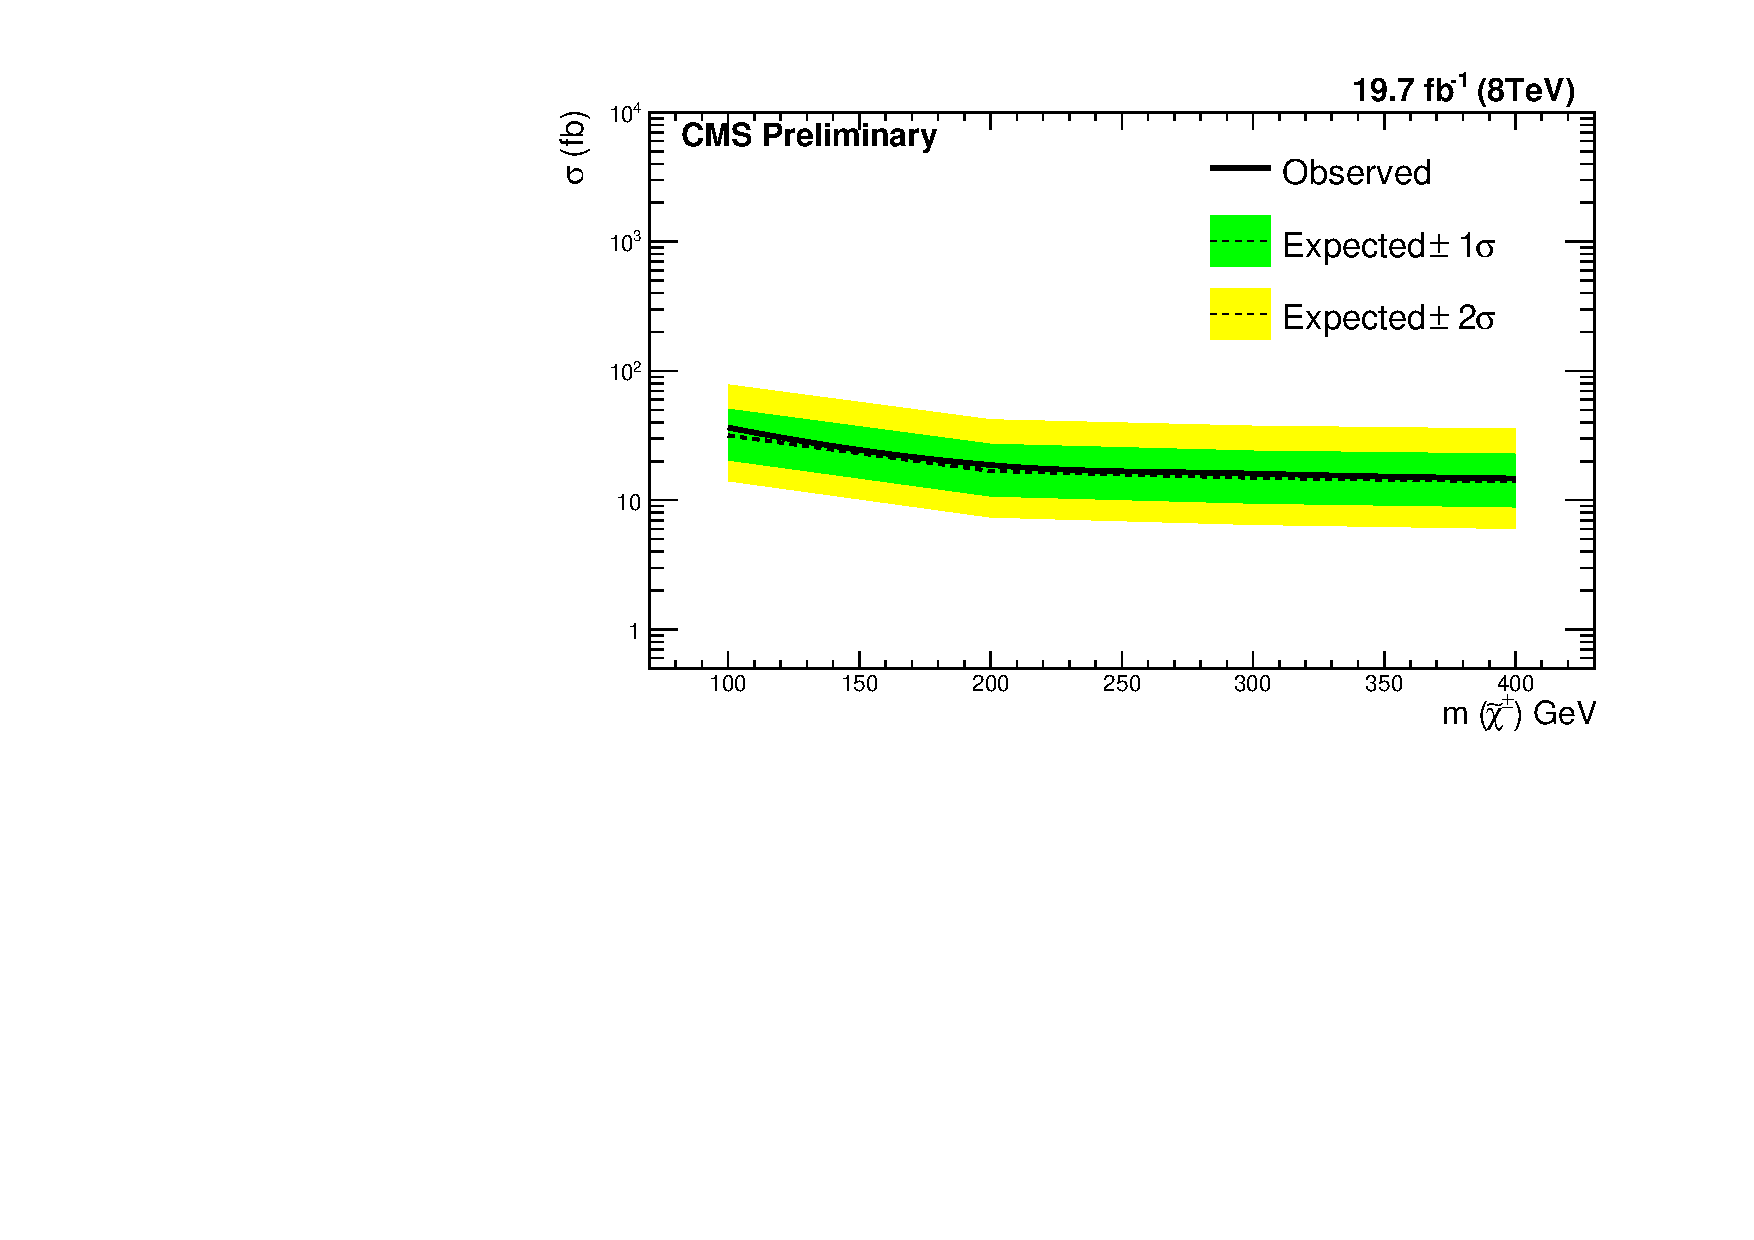
\includegraphics[angle=0,width=.48\textwidth, height=0.35\textheight]{PLOTS/Limit_VBF_diTau_LS.pdf}
    \caption{Upper limit at the 95\% CL on the cross-section as a function of 
$m_{\tilde{\chi}_{2}^{0}}=m_{\tilde{\chi}_{1}^{\pm}}$ for the (a) OS 
$\tau_{h}\tau_{h} j_{f} j_{f}$, (b) LS $\tau_{h}\tau_{h} j_{f} j_{f}$
final states. The bands represent the one and two standard deviations obtained from the background-only hypothesis.}
  \label{fig:LimitsOSLS}
 \end{center}
\end{figure}

\begin{figure}
  \begin{center}
    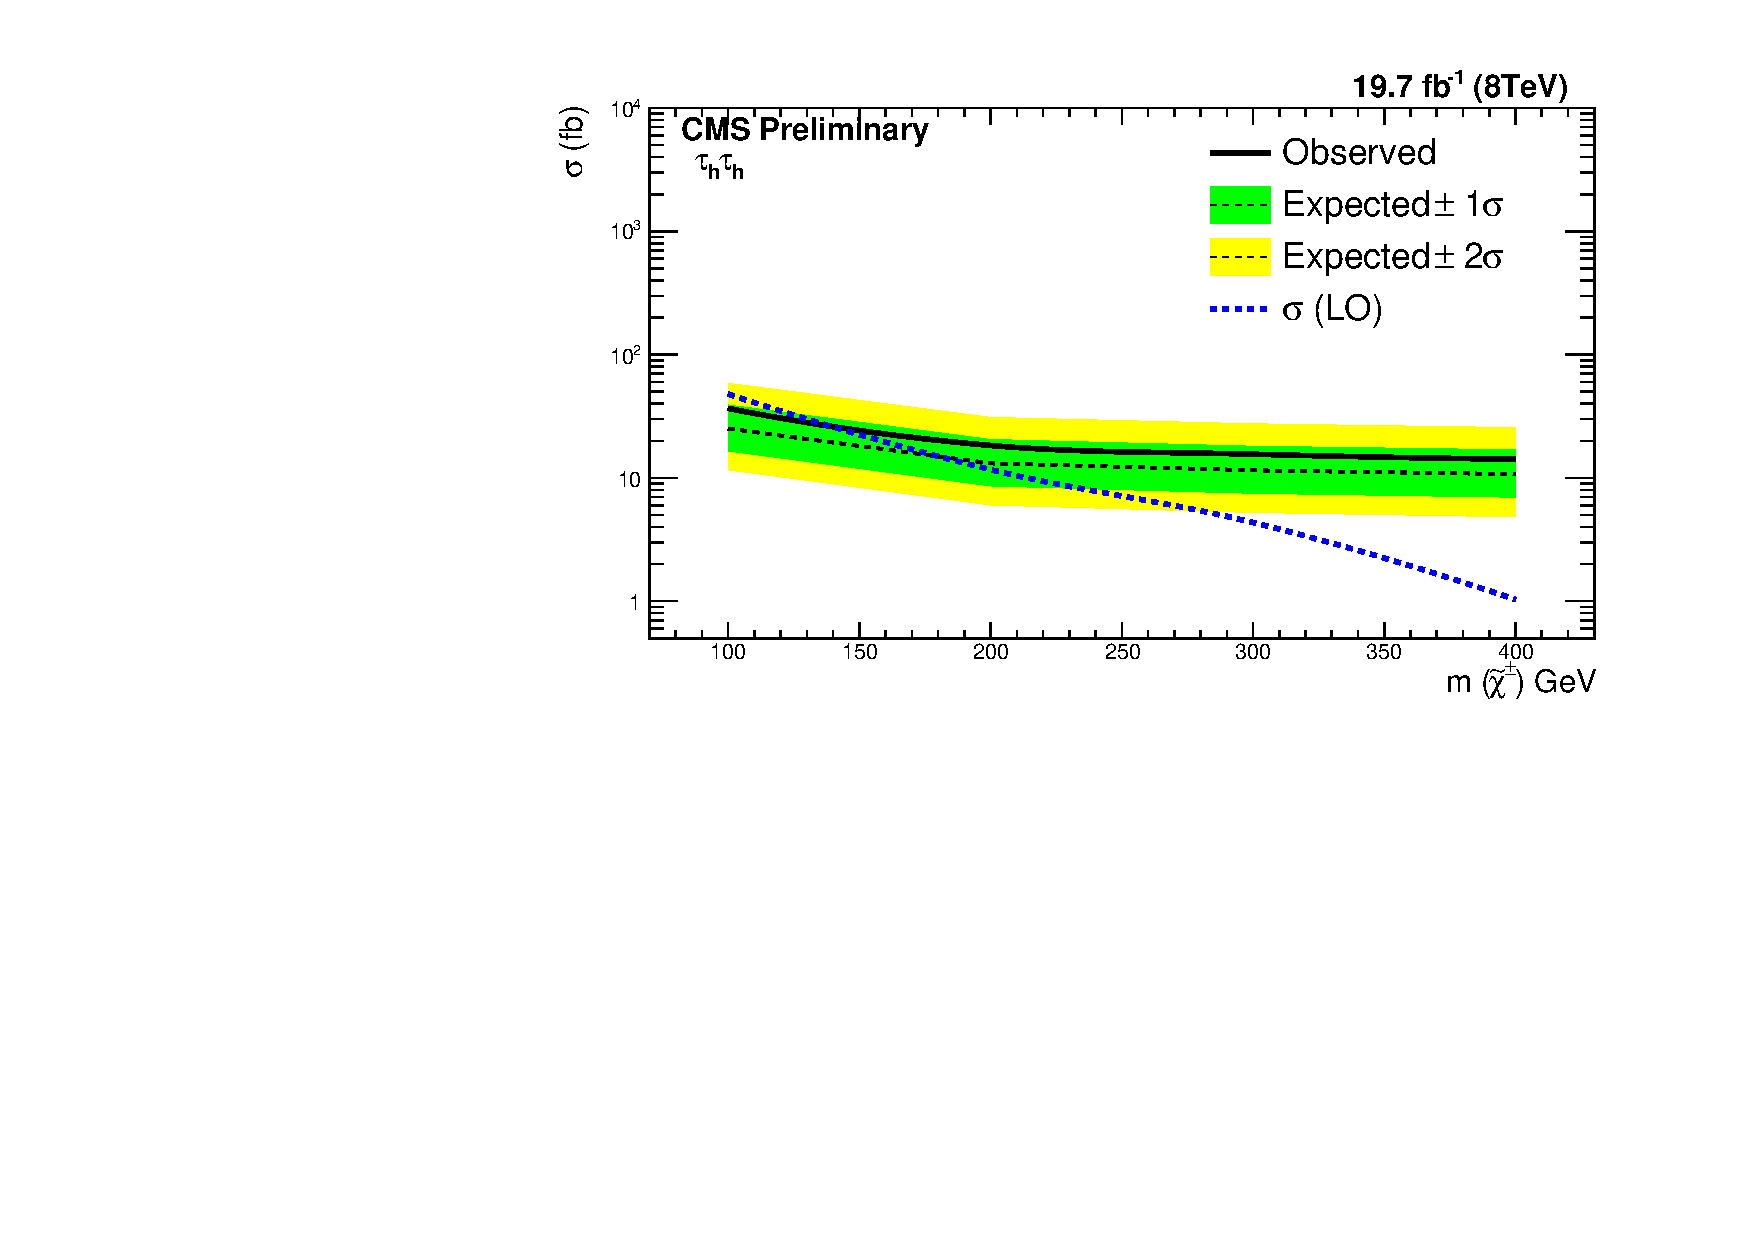
\includegraphics[angle=0,scale=0.8]{PLOTS/Limit_VBF_diTau_combined.pdf}
    \caption{Upper limit at the 95\% CL on the cross-section as a function of 
$m_{\tilde{\chi}_{2}^{0}}=m_{\tilde{\chi}_{1}^{\pm}}$ for the combination of OS and LS $\tau_{h}\tau_{h} j_{f} j_{f}$
final states. The bands represent the one and two standard deviations obtained from the background-only hypothesis.}
    \label{fig:LimitsCombination}
 \end{center}
\end{figure}

Figure \ref{fig:LimitsOSLS}(a) \ref{fig:LimitsOSLS}(b) and  shows the upper limit at the 95\% CL on the cross-section for OS and LS channel. A combination of the two channels is shown on Figure \ref{fig:LimitsCombination}. The upper expected limit on $m_{\tilde{\chi}}$ corresponds to the point where the expected limit crosses the theoretical line and is set for  $\tilde{\chi}_{1}^{\pm} /\tilde{\chi}_{2}^{0} $ with masses of 180 GeV. The upper observed limit on $m_{\tilde{\chi}}$ corresponds to the point where the observed limit crosses the theoretical line. We exclude $\tilde{\chi}_{1}^{\pm} /\tilde{\chi}_{2}^{0} $ with masses below 140 GeV in the models considered. The limit results coming from OS and LS $\tau_{h}\tau_{h} j_{f} j_{f}$ final states are combined with other 6 channels documented on AN-12-321 for the final upper limit.



\cleardoublepage

\chapter{SUSY VBF Studies at 13 TeV}
\label{sec:13TeVanalysis}


After two years of maintenance and upgrades, LHC started the second run phase, also known as \textit{Run2}, in 2015 featuring an increase of the center of mass energy up to 13\tev. The goal of this run is to increase the delivery of particle collisions for physics research, and thereby speed the route to potential new physics. A considerable upgrade program has been planned also for the CMS ad ATLAS detectors, featuring the upgrades of many sub-detectors and software tools. It is possible to study the capabilities that searches for SUSY events in vector boson fusion events have using the new hardware and software setup. This chapter describes a sensitivity study of a SUSY VBF search performed using 13\tev simulated data.

\section{Signal and background samples}

The signal event samples are generated with the \texttt{MadGraph v5.2.1} program \cite{Alwall:2011uj}, considering pair production of gauginos with two associated partons. The signal events are generated requiring a pseudorapidity gap $|\deltaeta| > 4.2$ between the two partons, with $\pt > 30\gev$ for each parton. The signal samples have been generated following all the considerations made for 8\tev analysis for \charginopm = \neutralinotwo masses of 100, 200, 300 and 500\gev. Two are the assumptions made to fix the \stau mass: the fixed-mass and average-mass assumptions. For each of those assumption two different scenarios has been taken into account: the uncompressed mass spectrum and the compressed mass spectrum scenarios.

The Monte Carlo background events used in this study refer to the production run labeled as \texttt{RunIISpring15MiniAODv2} and incorporate the \texttt{CTEQ10} \cite{Dulat:2013hea} parton distribution functions (PDF).The \texttt{POWHEG} and \texttt{MadGraph} generators are interfaced with the \texttt{PYTHIA v8.5.12} \cite{Sjostrand:2006za} program, which is used in the matching between the matrix elements, the parton shower, and the hadronization processes. 

All the Monte Carlo samples are stored in a new format called \texttt{miniAOD} \cite{bib:WorkBookMiniAOD}. This format is an updated version of the previously used one and includes the new CMS reconstruction features developed between the time of the original analysis and the starting of Run2. A comprehensive list of all the samples used in this study is listed in \autoref{sec::sampleslist_13tev}.

\section{Object reconstruction}

The upgrade plan commissioned for the CMS detector translates also into an updated version of the physical object definition used for this study with respect to the one used in the 8\tev analysis.

The \hadtau object reconstruction went through a major update with the introduction of new isolation and decay mode discriminators and electron veto \cite{bib:TauID_13tev}. Its reconstruction has been commissioned for $\pt > 20$\gev in all $\eta$ ranges. Using the specifications suggested by the Tau POG, an increase of the overall TauID efficiency of about 10\% for loose isolated \hadtau with respect to the 8\tev specifications is achieved, with the reconstruction efficiency going up to 71\% for $Z \longrightarrow\tau\tau$ events\cite{bib:TauID_13tev}. A detailed list of the \hadtau object selection can be found in Table \ref{table:tauobjdefinition_13TeV}. 

The Jet object definition remained unchanged with respect to the one used in the 8\tev analysis.  

With Run 2 the experiment gains access to a new trigger list. The aim is to use a trigger that is exclusively making an online selection on the dijet object kinematic properties. Differently with respect to the 8\tev trigger version, this trigger cannot be seeded by a level one trigger based on \met. The drop of all online selections over the \hadtau properties leads to some important advantages. First, it is possible to have a lower \hadtau \pt selection. Second, it is possible to go from a 1-prong to a 3-prong decay selection since this stringent requirement is not a part of any level 1 trigger seed. 

The b-tag object reconstruction has an updated discriminator as suggested by the POG \cite{bib:BJetID_13tev}.

\section{Cross section limit studies}

The aim of this study is to optimize the event cuts is order to exclude signal at the lowest cross section measurable. A cross section limit is made by requiring the so called significance $\alpha$ to:

\begin{equation}
\alpha = 2
\label{eq::significance_xsec_limit}
\end{equation}

There are several definitions of significance $\alpha$ available in literature, however the one picked for this 13\tev study is a frequentist definition based on completely standard concepts\cite{Punzi:2003bu} which is generally applicable, and has a very clear interpretation. It is particularly suitable for optimization, being independent of a-priori expectations about the presence of a signal, thus allowing the determination of a single set of cuts that is optimal both for setting limits and for making a discovery. The definition of sensitivity is:

\begin{equation}
\alpha = \dfrac{S}{\dfrac{a}{2} + \sqrt{B + \left( \dfrac{B}{2}\right)^{2}}}
\label{eq::punzi_formula}
\end{equation}

with $a$ the confidence level expressed in terms of $\sigma$, and $S$ and $B$ the number of signal and background vents for a given selection. One of the most important features of \autoref{eq::punzi_formula} that it is non-diverging in case of $B = 0$.

The number of signal events can be defined as:

\begin{equation}
S = \epsilon \cdot \sigma_{sec} \cdot L
\label{eq::punzi_signal_events}
\end{equation}

where $\epsilon$ is the efficiency for a given selection criteria, $\sigma_{sec}$ the cross section of the signal process considered and $L$ the luminosity given by the experiment. Is it possible now to define the efficiency $\epsilon$ as function of variables used in the analysis event selection. Three of the most important variables in the 8\tev analysis has been chosen for this study: $\pt(\hadtau)$, \met and $m_{jj}$. The definition of $\epsilon$ in \autoref{eq::punzi_signal_events} now becomes:

\begin{equation}
\epsilon^{signal} ( \pt(\hadtau) , m_{jj} ,  \met ) = \dfrac{N^{signal}_{passed}(\pt(\hadtau) , m_{jj} ,  \met)}{N^{signal}_{total}}
\label{eq::punzi_efficiency}
\end{equation}

where $N^{signal}_{passed}$ is the number of signal events passing the selection criteria as a function of the chosen variables and $N^{signal}_{total}$ is the total number of signal events. It is easy to notice that by fixing the significance value as shown on \autoref{eq::significance_xsec_limit} the cross section $\sigma_{sec}$ in \autoref{eq::punzi_signal_events} becomes indeed the cross-section limit $\sigma^{lim}_{sec}$. After merging both \autoref{eq::punzi_signal_events} and \autoref{eq::punzi_efficiency} the cross section limit $\sigma^{lim}_{sec}$ is defined as:
	
\begin{equation}
\sigma^{lim}_{sec}( \pt(\hadtau) , m_{jj} ,  \met ) = \dfrac{\alpha \cdot\left(\dfrac{a}{2} + \sqrt{B( \pt(\hadtau) , m_{jj} ,  \met ) + (0.5 \cdot B( \pt(\hadtau) , m_{jj} ,  \met ))^{2}}\right)}{\epsilon^{signal} ( \pt(\hadtau) , m_{jj} ,  \met ) \cdot L}
\label{eq::xsec_lim}
\end{equation}



\subsection{Event selection}
\label{subsec::event_sel_13tev}

The values for $\epsilon^{signal}$ and $B$ are directly taken from the signal and background samples listed in \autoref{sec::sampleslist_13tev}, on which the event selection has been applied. The idea of this 13\tev study is to be as close as possible to the one done in 8\tev, therefore the event selection is very similar to the one described in \autoref{sec:eventselection}.

As previously mentioned the event selection for this study is a function of the reconstructed tau \pt , \met and the di-jet candidate invariant mass $m_{jj}$, therefore those cuts are considered as free variables in the event selection. 

The uncertainties on the official 13\tev trigger list and on how good are those triggers simulated in Monte Carlo lead to the decision of removing the trigger requirement in the event selection. In case this study will use 13\tev data it is useful to notice that a choice of a VBF-selection-seeded trigger will lead to an online selection over the di-jet canditates invariant mass $m_{jj}$.

The di-jet \deltaeta cut has been removed due to its strong correlation to the di-jet canditates invariant mass $m_{jj}$ as shown in the 8\tev study \cite{Khachatryan:2015kxa}.

For better visualization and understanding, all the selection criteria are summarized below:

\begin{itemize}
	\item \textbf{Central selection}
	\begin{itemize}
		\item two one-prong hadronically decaying $\tau$ with $\pt = 20,25,30,35,40,45\gev$
		\item at least two jets with $p_{T}^{jet}\geq30~$\gev, $|\eta_{jet}|\leq5$ and loose jetID
		\item $\Delta R(jet,\tau)\geq0.3$
		\item b-tag veto
	\end{itemize}
	\item \textbf{VBF selection}
	\begin{itemize}
		\item $\text{sign}(\eta^{jet 1}\cdot\eta^{jet 2})=-1$
	\end{itemize}
\end{itemize}

\subsection{Background estimation}

Similar to the analysis at 8\tev, the largest challenge for this study is to determine the number of background events in the signal region. As described in \autoref{sec::bg_contributions}, the main background contribution is coming from QCD events. The remaining background contributions are considered negligible. Even though this study is characterized by a loosening of the selection cuts with respect to the previous analysis, the limited statistics of the Monte Carlo samples used gives a very scarce number of selected events. The problem of a limited statistics is solved by estimating the number of background events in the signal region through a two-fold ABCD method. It involves the usage of two distinct correction factors in order to gradually convert the number of background events, taken from a starting control region with looser cuts, into the signal region ones. This method is defined under the same assumptions made for the 8\tev analysis, listed in \autoref{sec:bgestimation}.

Bearing in mind the idea of developing a method similar to the one used for 8\tev, the regions are defined by two distinct variables: the isolation of the di-tau candidates and the inversion of the VBF cuts. There are three regions defined for this method. The signal region, also called SR, is defined as the region fulfilling all the cuts listed in \autoref{subsec::event_sel_13tev}. Control region two, also called CR2, has the same selection as the one for the signal region but requires the inversion of the VBF-related cuts. Finally control region three, also called CR3, has the same selection as CR2 but requires the di-tau candidates to have a Loose isolated and a non-isolated \hadtau.

\begin{figure}[tbh!]
	\centering
	\begin{tabular}{cc}
		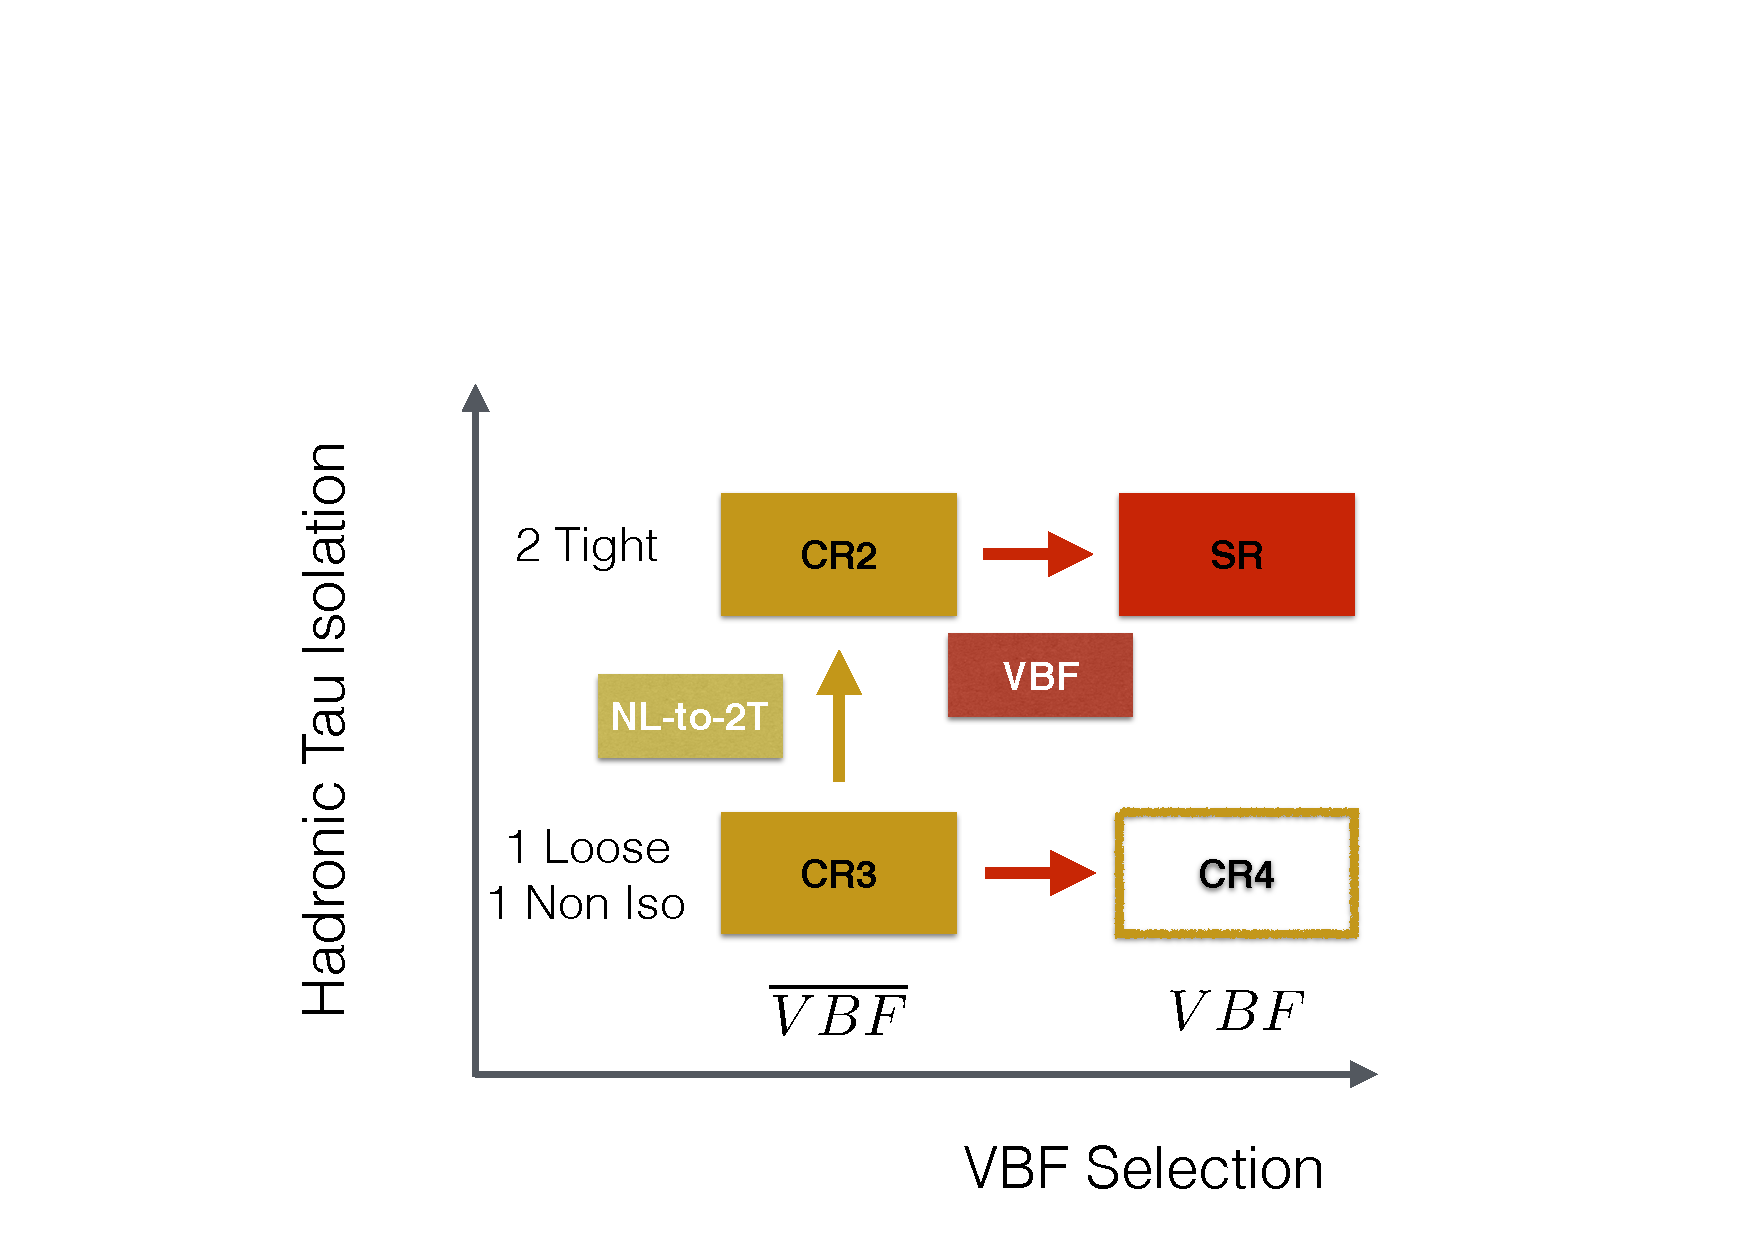
\includegraphics[width=0.75\textwidth]{PLOTS/diTauHadLSotherPlots/controlregions13TeV.pdf}
	\end{tabular}
	\caption{Definition of Signal and Control Regions using different $\hadtau$ isolation criteria and VBF selection.}
	\label{fig:crs_13tev}
\end{figure}

As previously mentioned, two conversion factors are used in this method. The first factor, named "\textit{NL-to-2T}" or "\textit{None-Loose to two Tight}", allows to convert the number of selected events from CR3 to CR2. This factor is derived from a study over the same QCD sample where the event population is high by only requiring at least four reconstructed jets in the event, and is defined as:

\begin{equation}
\text{NLto2T} = A \cdot B
\end{equation}

where $A$ and $B$ are ratios. Further, $A$ has as denominator the number of events with at least four jets where at least one of these jets is matched with a loose isolated \hadtau. In case this matched \hadtau is also tight isolated the events are counted in the numerator:

\begin{equation}
A = \dfrac{N_{events}(\text{the matched }\hadtau\text{ is also tight isolated })}{N_{events}(= 1\text{jet matched to loose }\hadtau)}
\end{equation}

The definition of $B$ is equal to $A$ with the only difference that the \hadtau matched to a jet in the denominator is non-isolated:

\begin{equation}
B = \dfrac{N_{events}(\text{the matched }\hadtau\text{ is also tight isolated })}{N_{events}(= 1\text{jet matched to non-isolated }\hadtau)}
\end{equation}

The second conversion factor is identical to the VBF conversion factor defined in \autoref{sec:bgestimation} with the only difference of the updated version of the VBF cuts for the 13\tev study. This factor is derived from the control regions with a lower \hadtau isolation requirements such as CR3 and CR4:

\begin{equation}
\text{VBF} = \frac{\epsilon^{QCD}_{VBF}}{1 - \epsilon^{QCD}_{VBF}}
\end{equation}

where $\epsilon^{QCD}_{VBF}$ is previously defined in \autoref{eq:vbfeff}. 

Finally the number of predicted events in the signal region is:

\begin{equation}
B = N^{QCD}_{SR} = N^{MC}_{CR3}  \cdot \text{NLto2T} \cdot \text{VBF}
\label{eq::qcdbgpred_13tev}
\end{equation}

A representation of the regions and the conversion factor used in this two-fold ABCD method is shown in \autoref{fig:crs_13tev}.

\subsection{Systematic and statistical uncertainties}

The uncertainty consider for this study originates from the simulated samples. Following the strategy used in the previous analysis this systematic uncertainty is estimated from the variation on the cross-section limit result after considering a $\pm 50\%$ variation of the Monte Carlo statistics.

\section{Results}

The definition of the cross-section limit $\sigma^{lim}_{sec}$, as given in \autoref{eq::xsec_lim}, allows a scan in a three-dimensional space defined by the variables $\pt(\hadtau)$ , \mjj and \met. The minimum cross-section limit found by the scan gives the optimal event selection cuts for each of the available signal benchmark points. The distribution of the most important analysis variables are shown in \autoref{fig::crplots1_Taui2TightIso_13tev_results}, \autoref{fig::crplots2_Taui2TightIso_13tev_results}, \autoref{fig::crplots3_Taui2TightIso_13tev_results} and \autoref{fig::crplots4_Taui2TightIso_13tev_results}; for this purpose the cuts over the study variables $\pt(\hadtau)$, \mjj and \met have been removed. 

For an easier reading over the results of the cross-section limit study, it is possible to simplify the three-dimensional problem in a "\textit{two plus one}" dimensional one. Following this approach, the cross-section limits are calculated and shown in a two-dimensional plot defined in bins of \mjj and \met. This process is then repeated for each of the chosen $\pt(\hadtau)$ cuts.

\begin{figure}[tbh!]
	\centering
	\begin{tabular}{cc}
		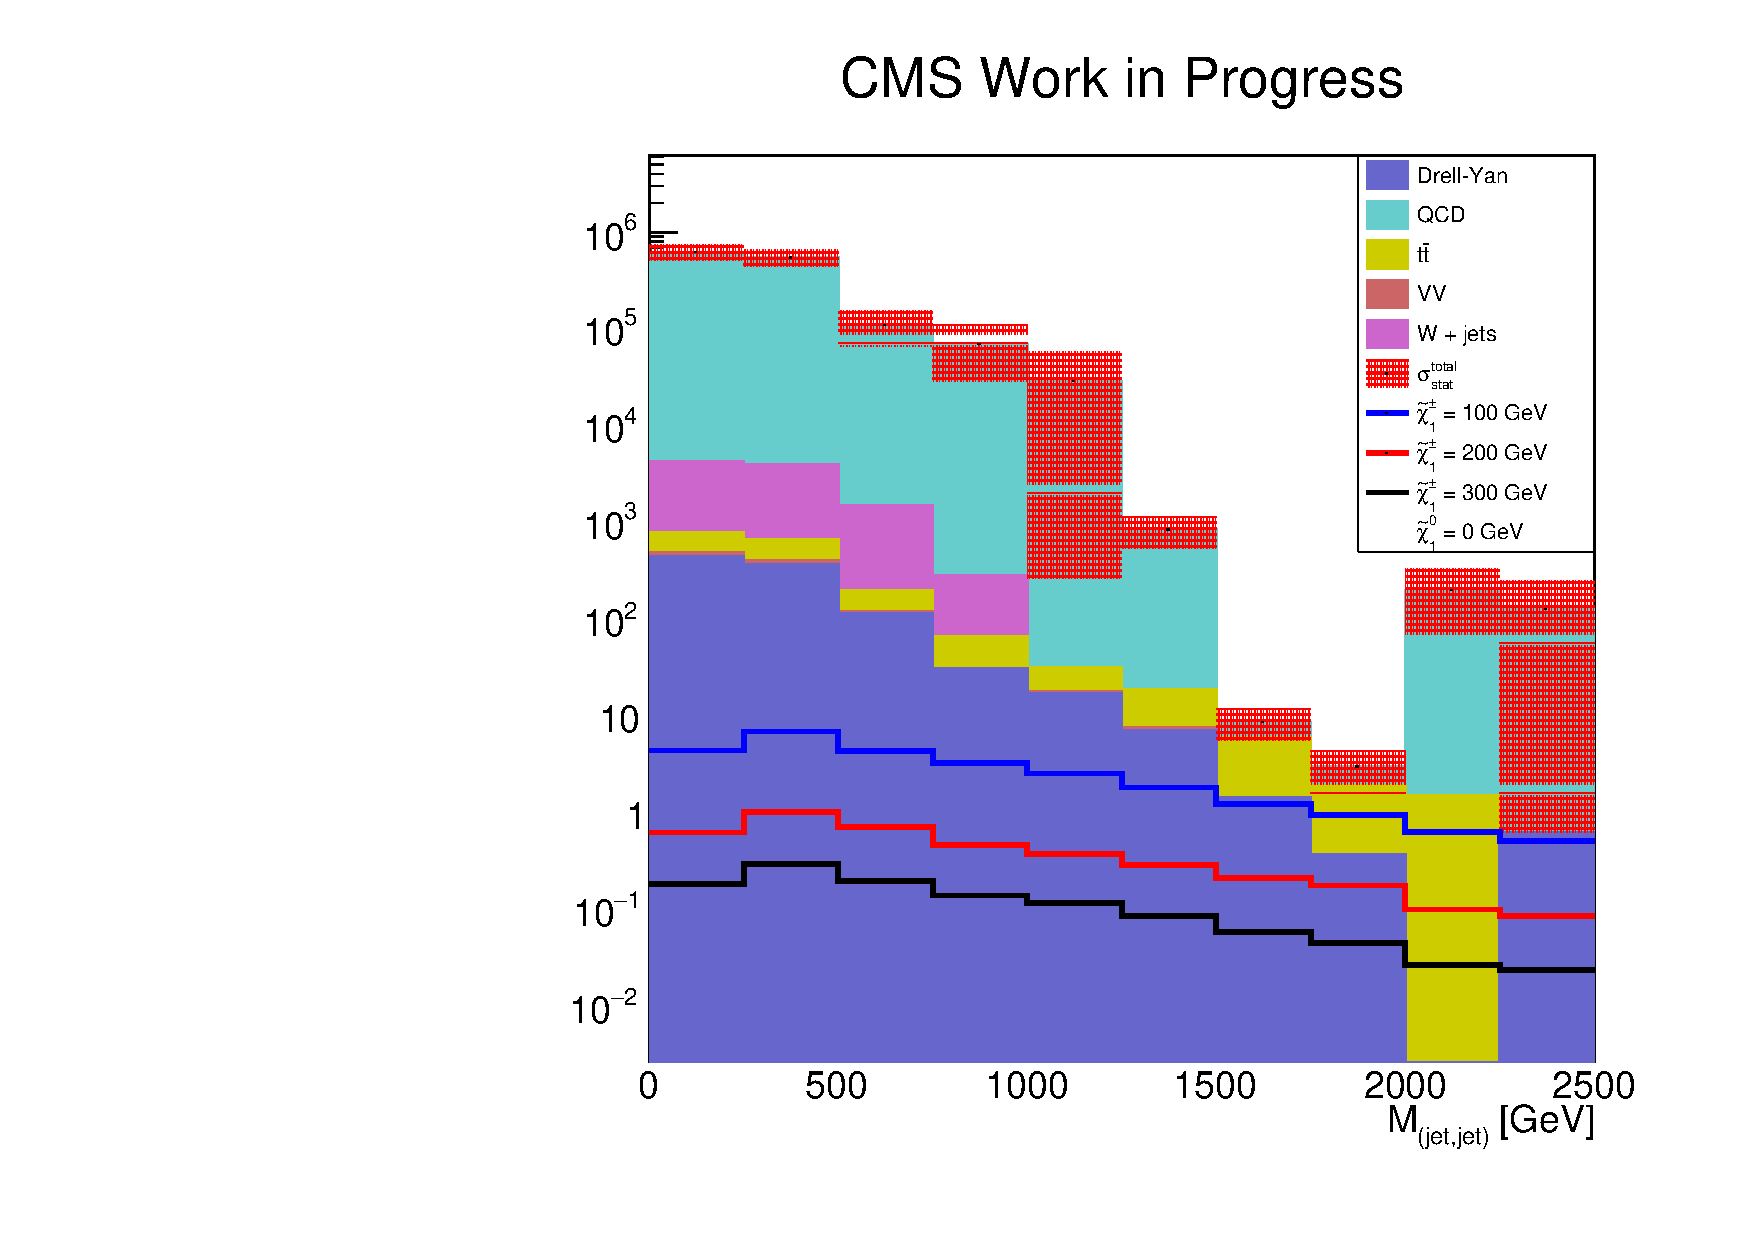
\includegraphics[width=0.5\textwidth]{analysis/pics/h_dijetinvariantmass_Taui2TightIso.pdf}
		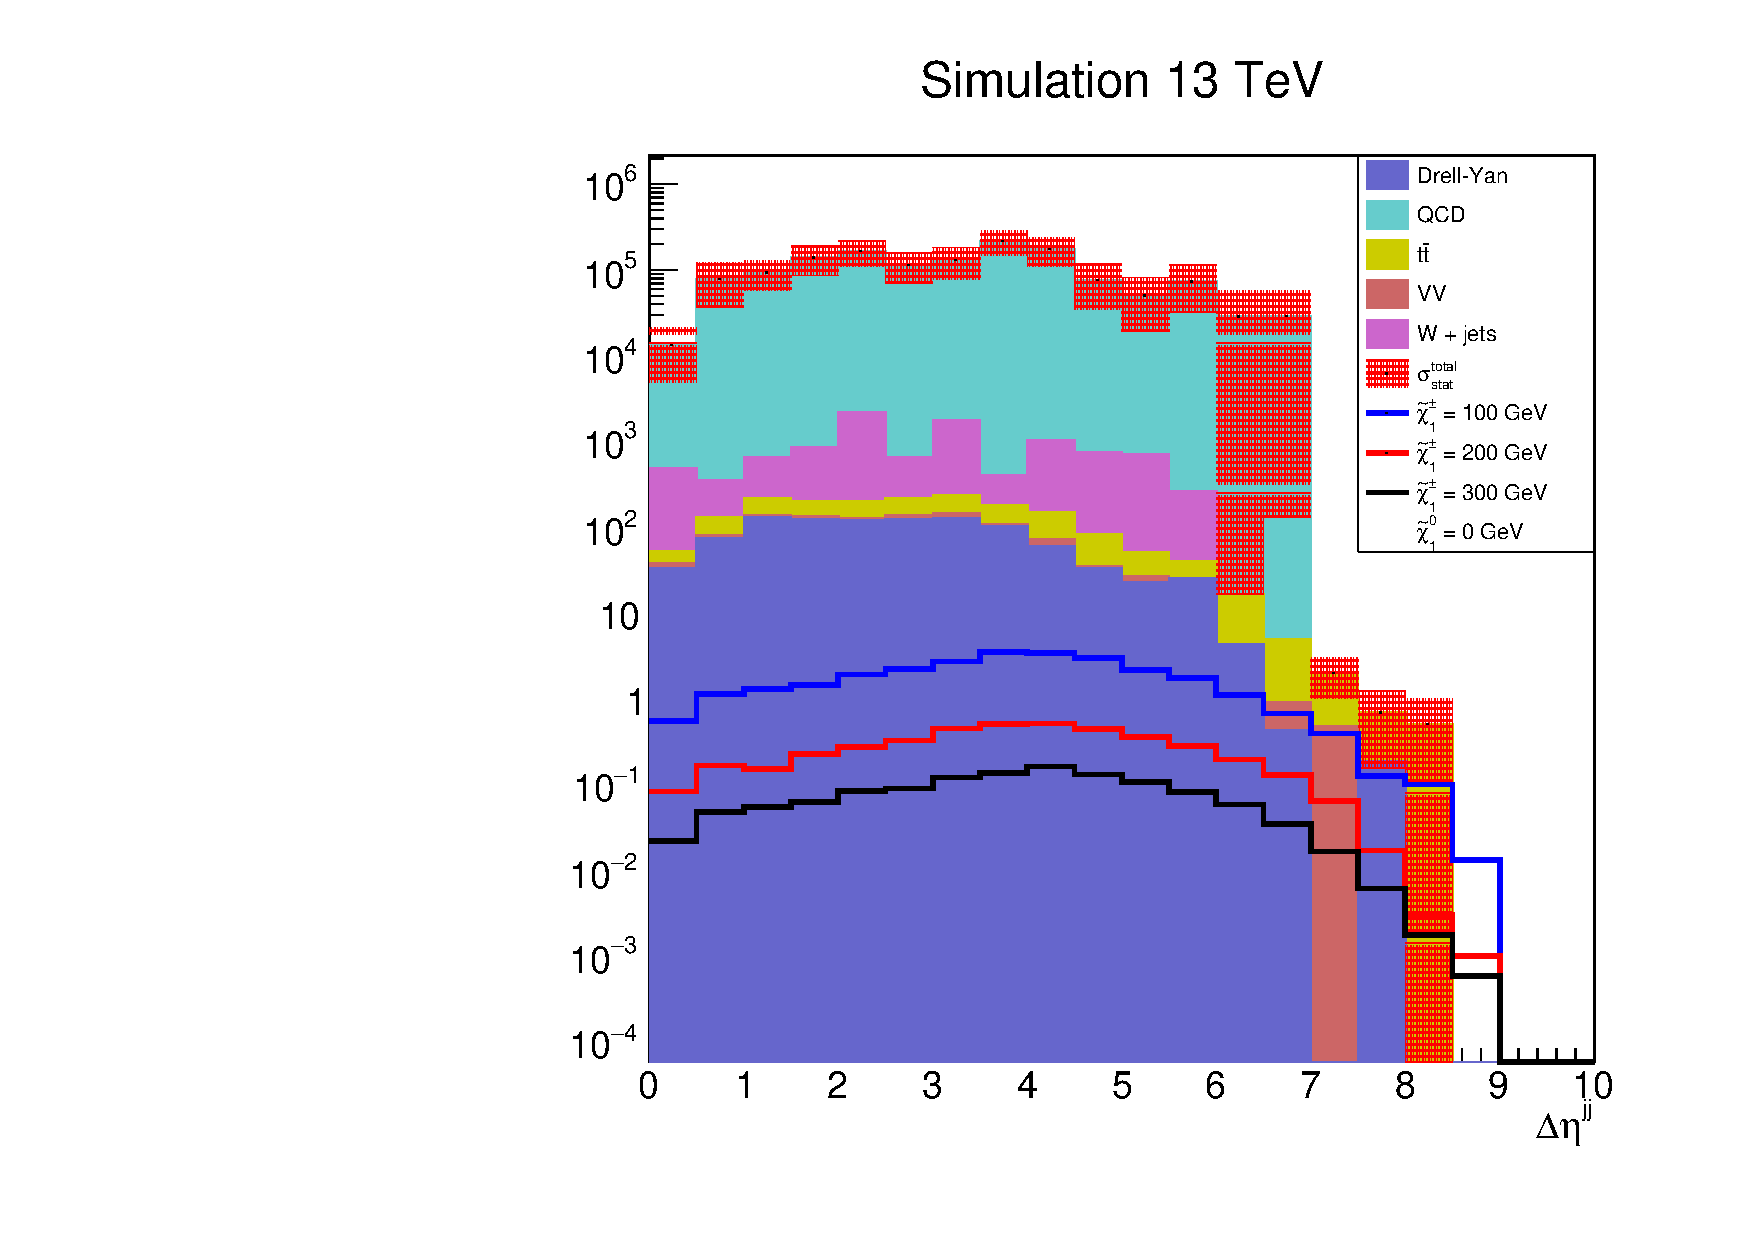
\includegraphics[width=0.5\textwidth]{analysis/pics/h_dijetdeltaeta_Taui2TightIso.pdf} 		
	\end{tabular}
	\caption{(Left) Di-jet invariant mass distribution and (Right) and Di-jet \deltaeta distribution of selected signal and all MC background samples in signal region.}
	\label{fig::crplots1_Taui2TightIso_13tev_results}
\end{figure}

\begin{figure}[tbh!]
	\centering
	\begin{tabular}{cc}
		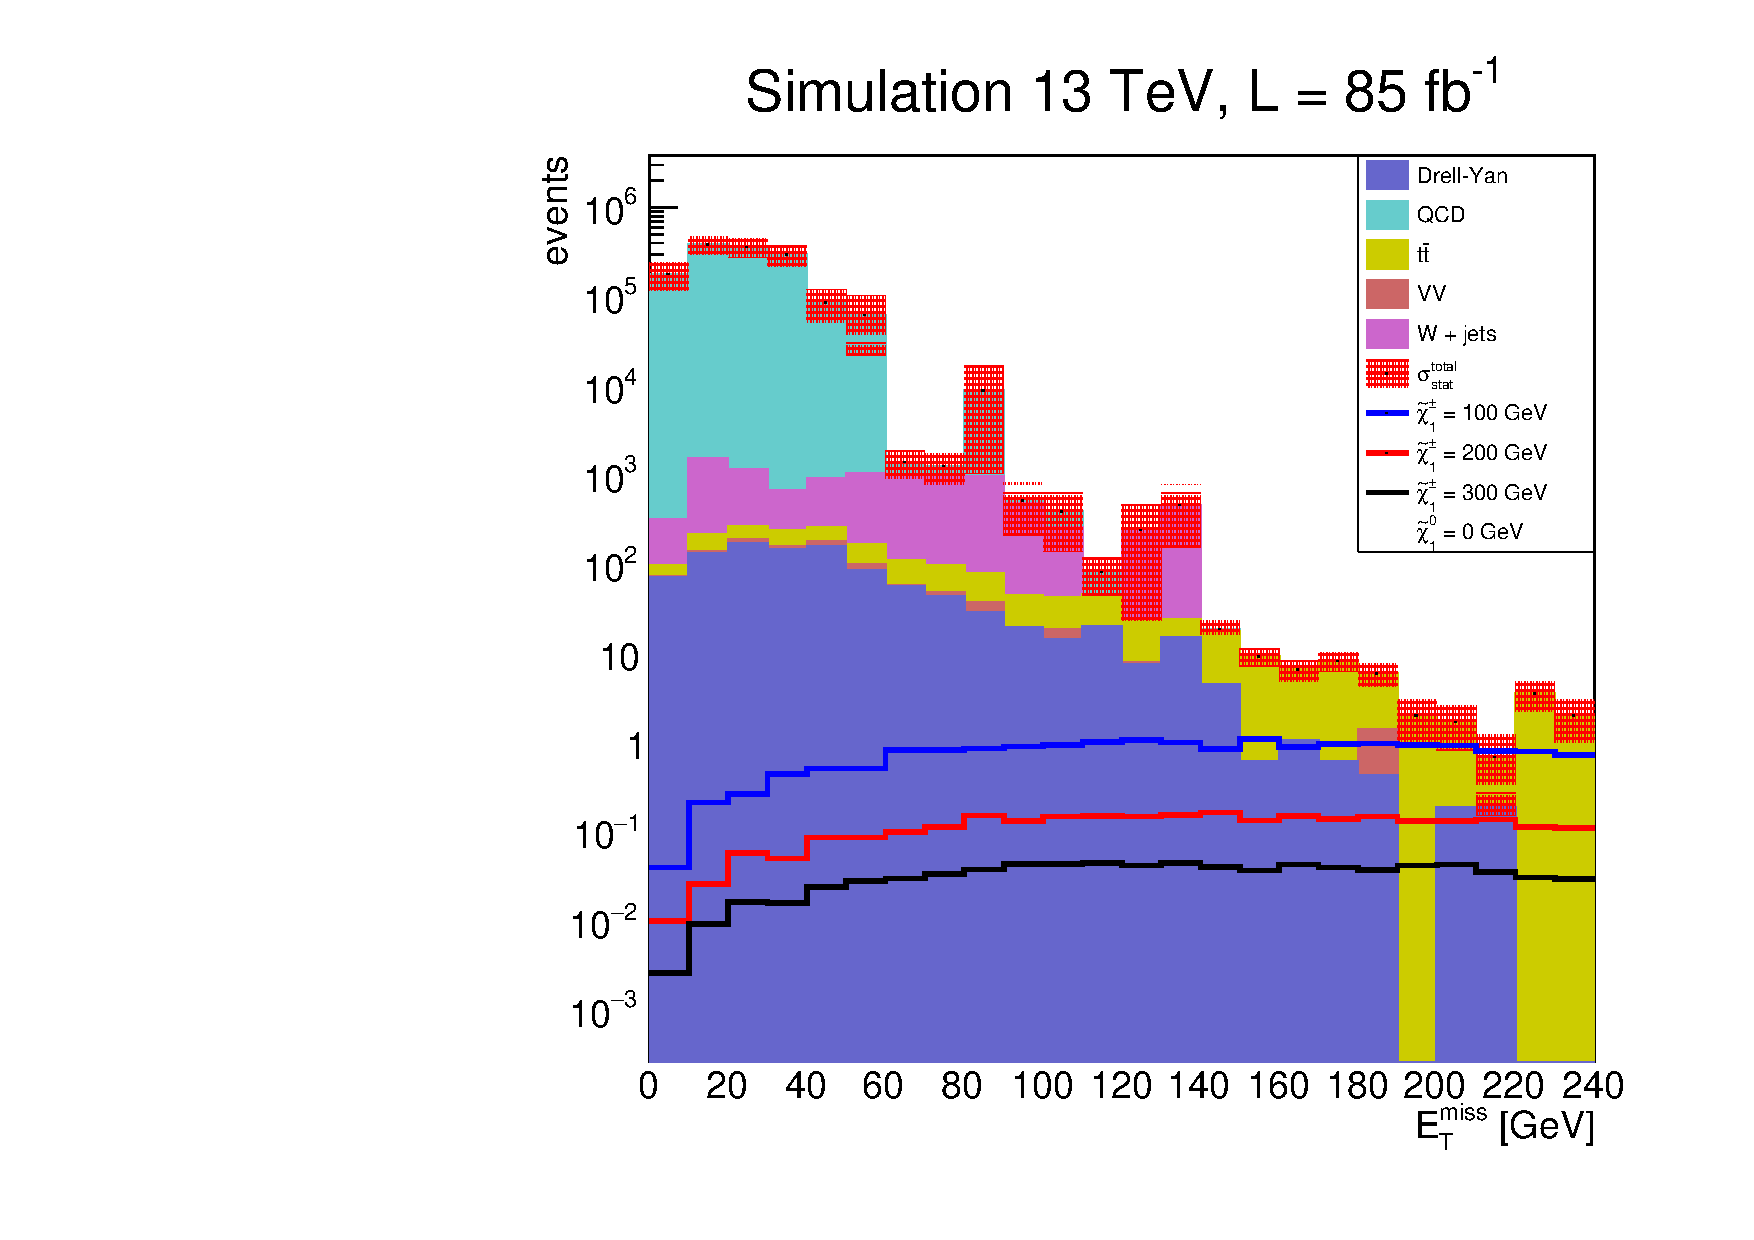
\includegraphics[width=0.5\textwidth]{analysis/pics/h_met_Taui2TightIso.pdf}
		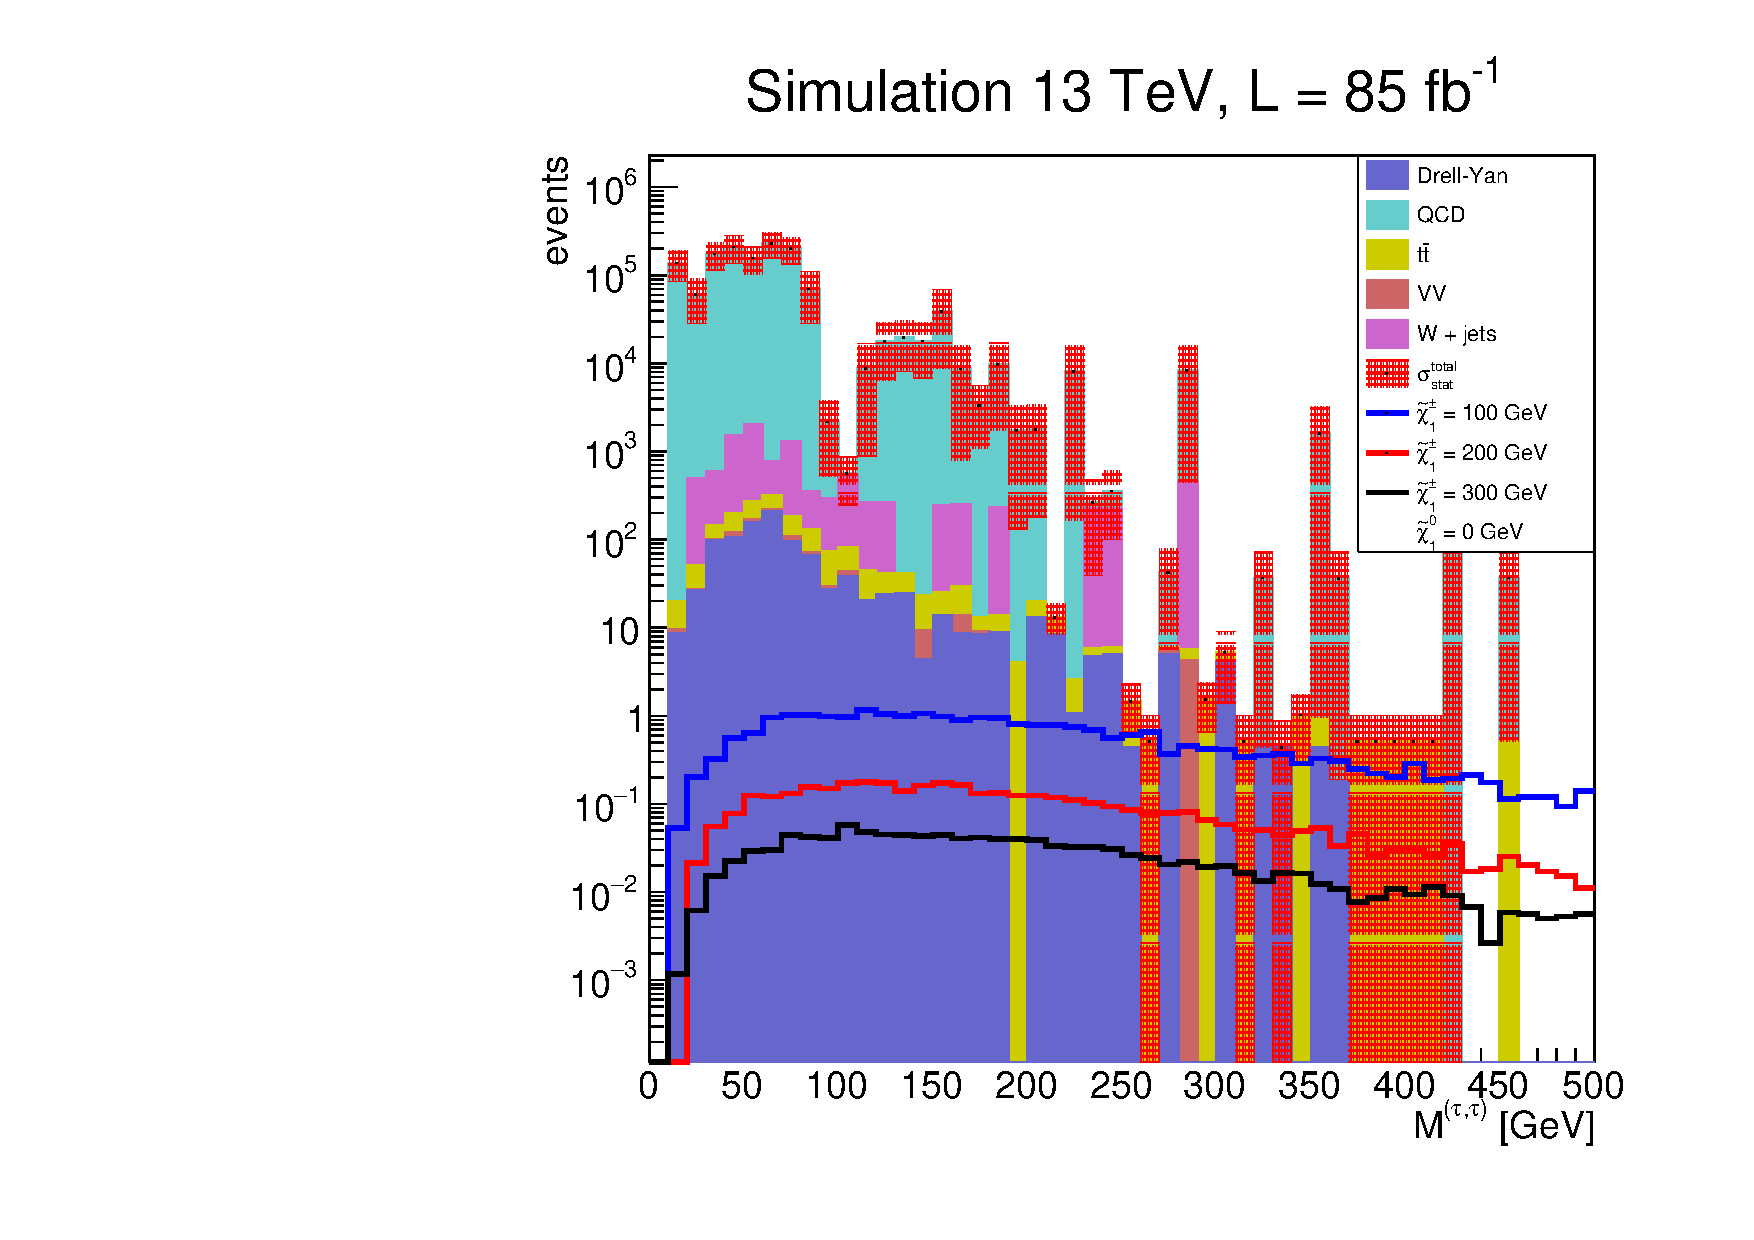
\includegraphics[width=0.5\textwidth]{analysis/pics/h_ditauinvariantmass_Taui2TightIso.pdf} 		
	\end{tabular}
	\caption{(Left) \met distribution and (Right) and Di-\hadtau invariant mass distribution of selected signal and all MC background samples in signal region.}
	\label{fig::crplots2_Taui2TightIso_13tev_results}
\end{figure}


\begin{figure}[tbh!]
	\centering
	\begin{tabular}{cc}
		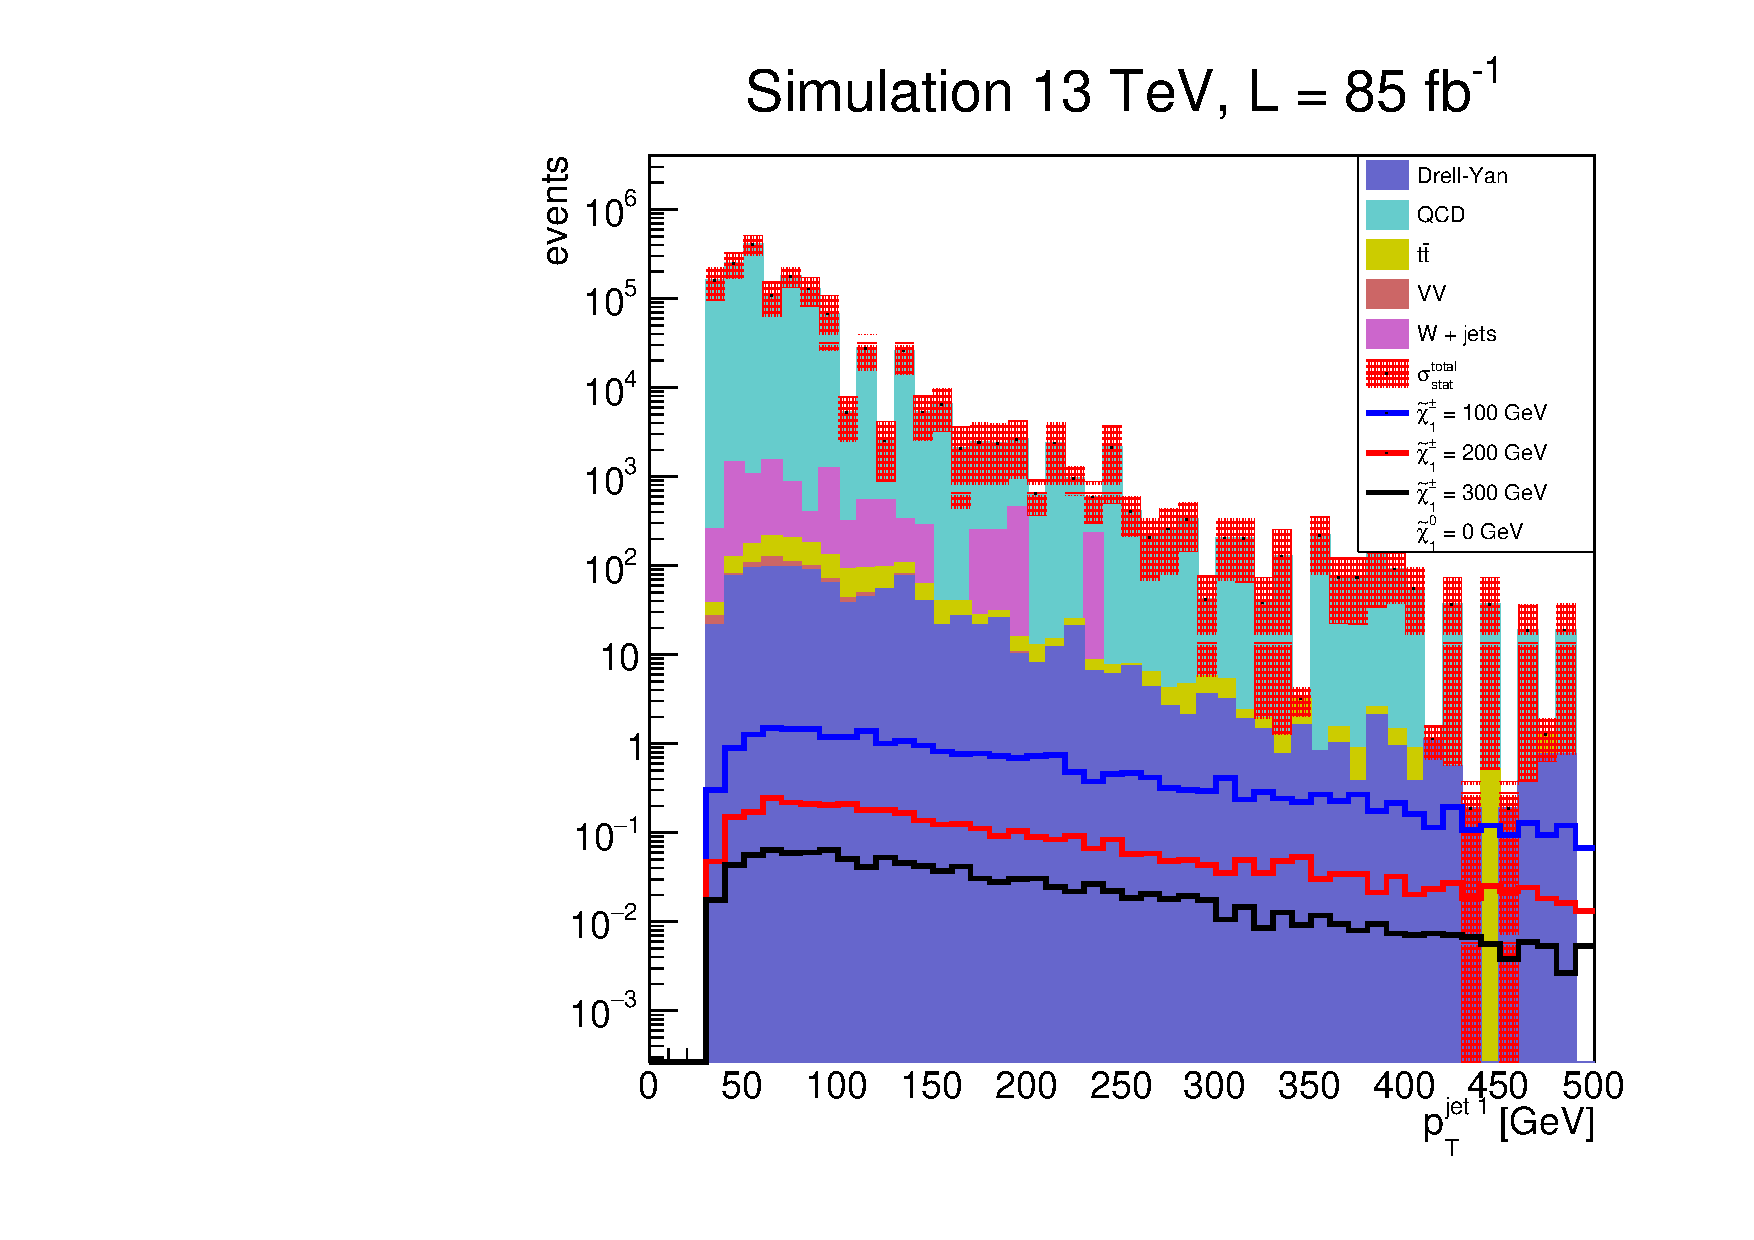
\includegraphics[width=0.5\textwidth]{analysis/pics/h_jet1pt_Taui2TightIso.pdf}
		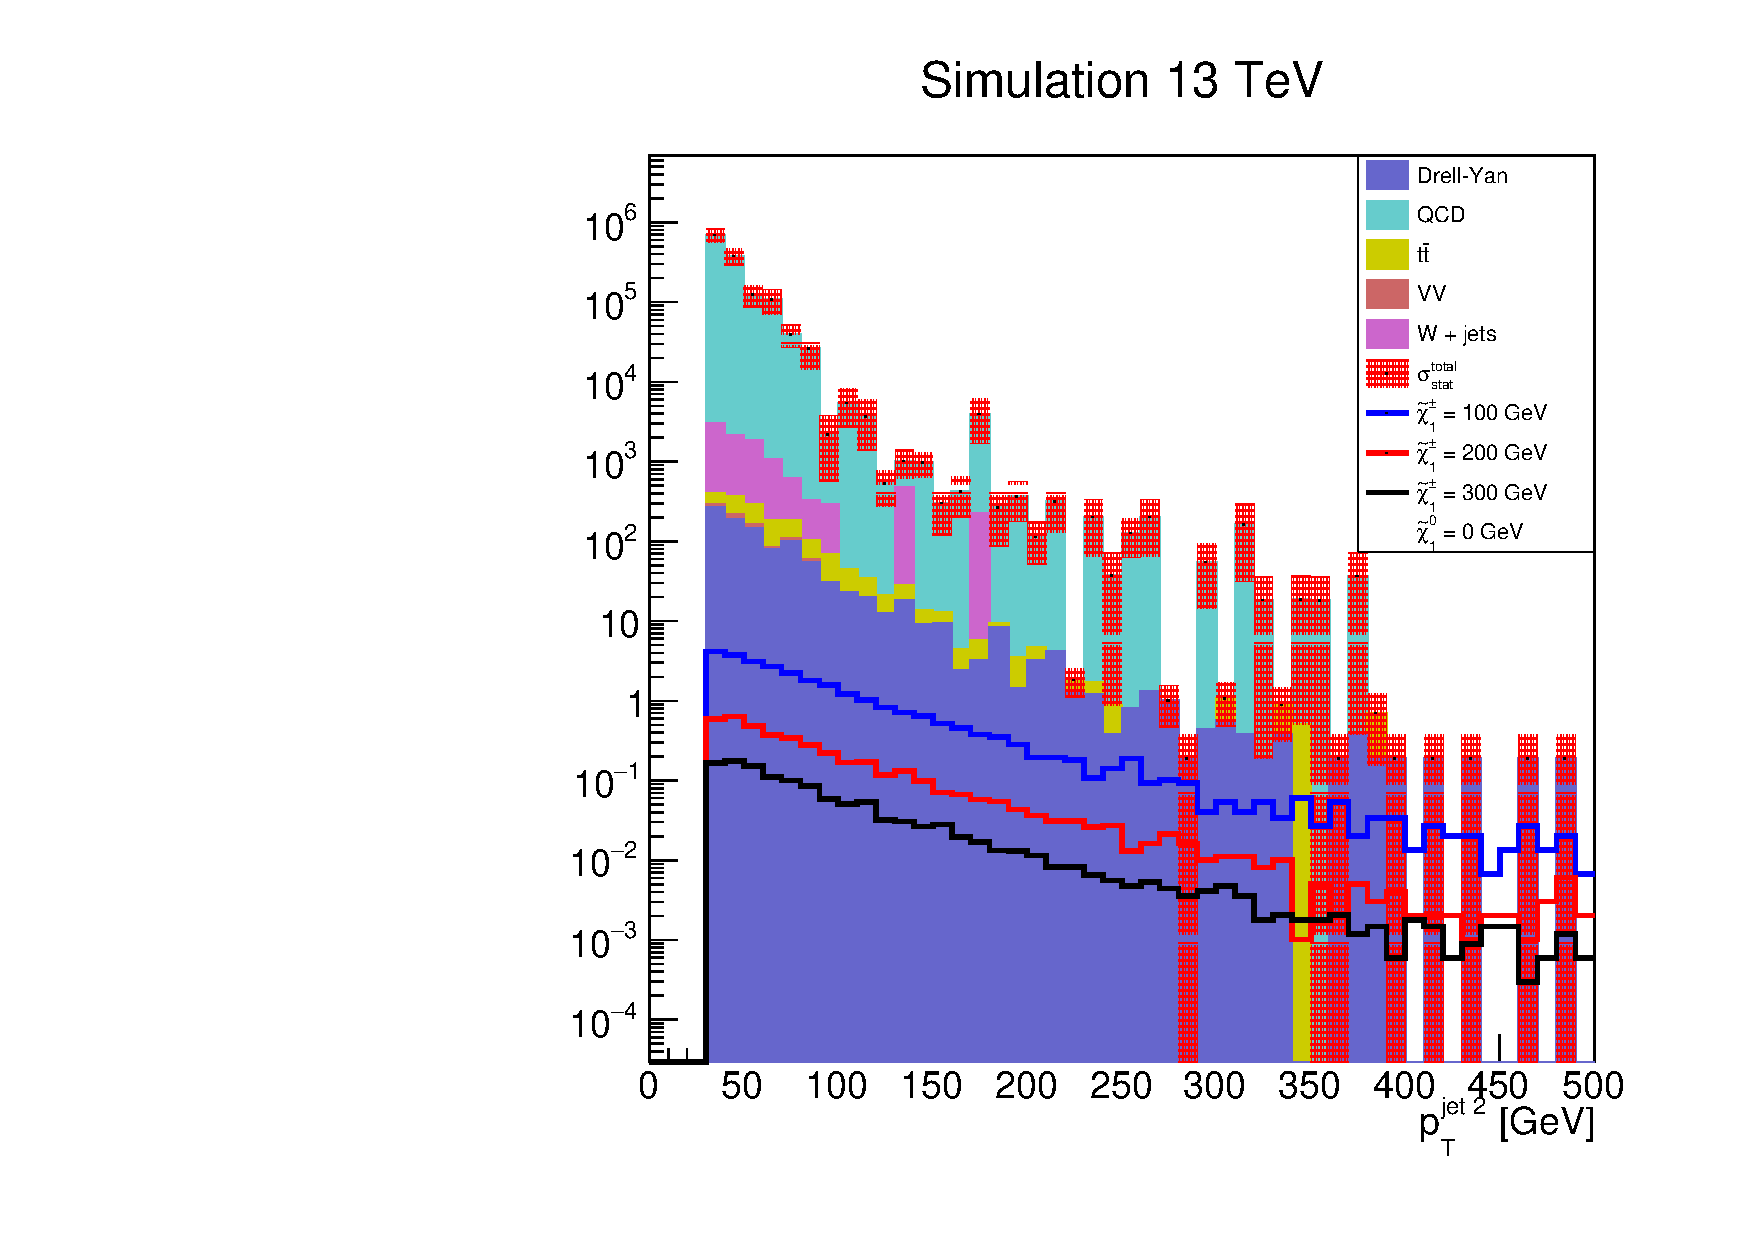
\includegraphics[width=0.5\textwidth]{analysis/pics/h_jet2pt_Taui2TightIso.pdf} 		
	\end{tabular}
	\caption{(Left) Leading jet \pt distribution and (Right) and second leading jet \pt distribution of selected signal and all MC background samples in signal region.}
	\label{fig::crplots3_Taui2TightIso_13tev_results}
\end{figure}

\begin{figure}[tbh!]
	\centering
	\begin{tabular}{cc}
		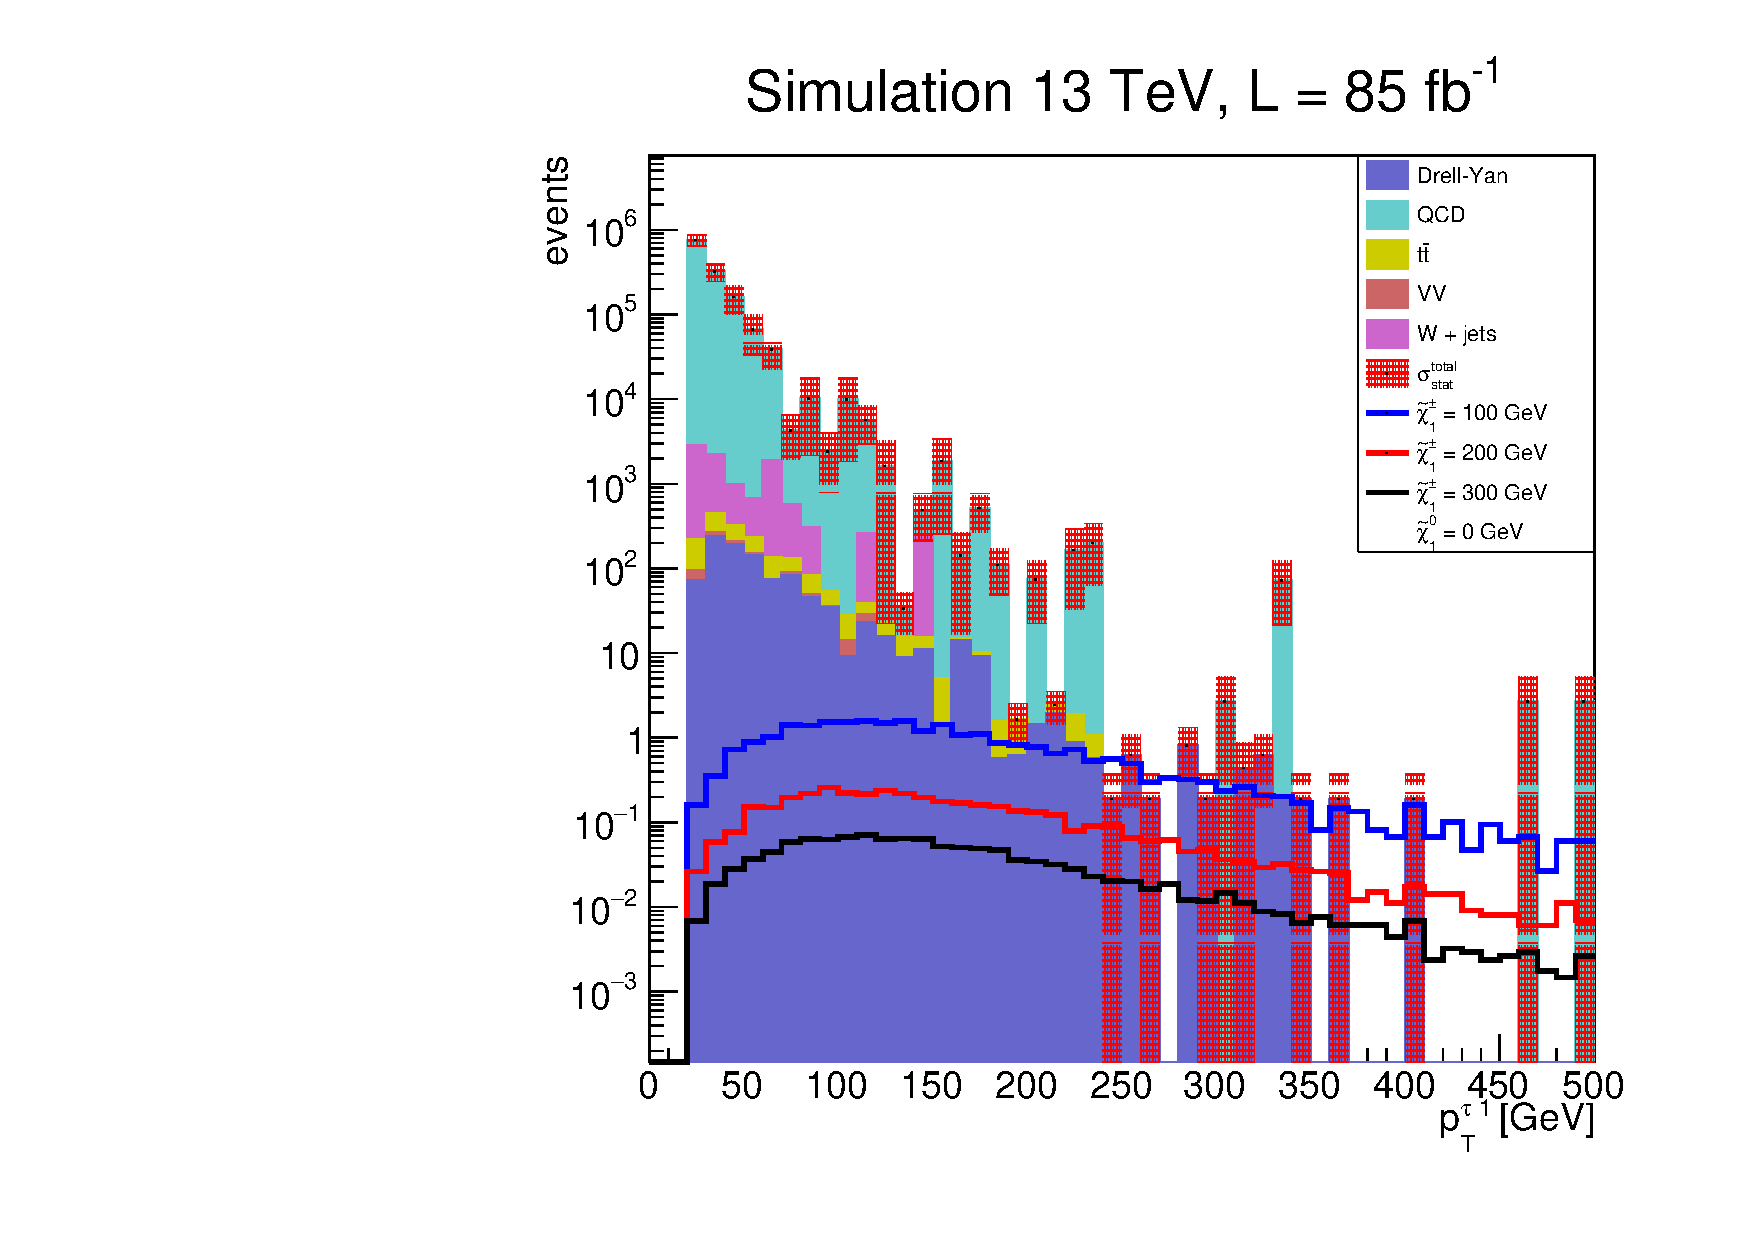
\includegraphics[width=0.5\textwidth]{analysis/pics/h_tau1pt_Taui2TightIso.pdf}
		\includegraphics[width=0.5\textwidth]{analysis/pics/h_tau2pt_Taui2TightIso.pdf} 		
	\end{tabular}
	\caption{(Left) Leading \hadtau \pt distribution and (Right) and second leading \hadtau \pt distribution of selected signal and all MC background samples in signal region.}
	\label{fig::crplots4_Taui2TightIso_13tev_results}
\end{figure}


Each of the two-dimensional bins stores a $\sigma^{lim}_{sec}$ for the given $\pt(\hadtau)$ , \mjj and \met cuts setup. The most important input values to \autoref{eq::xsec_lim} are the signal efficiency $\epsilon^{signal}$, as defined in \autoref{eq::punzi_efficiency},  and the number of predicted background events $B$, as defined in \autoref{eq::qcdbgpred_13tev}. The remaining input values are the luminosity $L$ and the confidence level $a$. The predicted luminosity for the 13\tev Run \cite{Bruning:2002yh} is estimated between 75 and 100\invfb; for the purpose of this study its value has been set to $L = 85\invfb$. The corresponding value as units of $\sigma$ with respect to a confidence level of 95\%  is $2$.

A full list of the study results is given as appendix in \autoref{sec::xseclim_results}. Similarly to what shown in the 8\tev analysis the cut over the $\pt(\hadtau)$ has an high impact on the signal efficiency $\epsilon^{signal}$; for an easier understanding of the final results this cut has been set to its allowed minimum of 20\gev.

The best cross-section limit scenario is given for a \charginopm and \neutralinotwo mass of 500\gev for the benchmark point assuming an uncompressed sparticles scenario and an average-\stau-mass assumption, as shown on \autoref{fig::xsec_lim_selected_results}. The cross-section limit minimum value is:

\begin{equation}
\sigma_{lim}^{min}\pm(stat.)\pm(MC syst.)\pm(VBF syst.) = 0.017\pm0.001^{+0.002 + 0.001}_{-0.002-0.000} [\text{pb}]
\label{eq::xsec_lim_best_result}
\end{equation}

for the optimal cuts of  $\pt(\hadtau) <  20\gev$,  $ \mjj< 500\gev $ and $\met < 250\gev$.

\begin{figure}[tbh!]
	\centering
	\begin{tabular}{cc}
		\includegraphics[width=0.75\textwidth]{analysis/pics/JetInvMass_vs_MET_xseclim_Chargino500_Stau250_LSP000_taupt20.pdf}
	\end{tabular}
	\caption{Cross section limit as function of $m_{jj}$ and \met for m(\charginopm) = m(\neutralinotwo) = 500 GeV,  m(\stau) = 250 GeV, and m(\neutralinoone) = 0 GeV and an offline selection on $\pt(\hadtau) <  20\gev$.}
	\label{fig::xsec_lim_selected_results}
\end{figure}

By comparing the 8\tev cross-section limit values with the ones at 13\tev it is possible to see that the previous analysis performs better in terms of limit setting as shown in \autoref{table::xseclim_7tev13tev_comparison}. The high statistical and systematic uncertainties shown for 13\tev are caused by the cut over the $\pt(\hadtau)$, which dramatically reduces the QCD statistics. It is worth to mention, however, that the 8\tev analysis has a selection which in general prevents the comparison in areas of the previously defined three-dimensional phase-space where the 13\tev analysis is meant to perform better thanks to the more gentle \hadtau candidate selection.

\begin{table}
\begin{center}
\begin{tabular}{| c | c | c | }
	\toprule
	\multicolumn{3}{| c | }{For $\pt(\hadtau) <  45\gev$  $\met > $ 30, $\mjj>250~$\gev, m(\neutralinoone) = 50\gev} \\
	\midrule
	m(\charginopm) = m(\neutralinotwo)  & $\sigma_{lim}^{min}\pm(stat.)\pm(syst.)$ [pb] (8\tev) & $\sigma_{lim}^{min}\pm(stat.)\pm(syst.)$ [pb] (13\tev)\\
	\midrule
   100\gev &  $0.084\pm0.016^{+0.18}_{-0.01}$ & $0.60\pm0.69^{+1.62}_{-0.87}$  \\
   200\gev &  $0.14\pm0.02^{+0.03}_{-0.04}$ & $0.65\pm0.74^{+1.74}_{-0.94}$ \\
   300\gev &  $1.43\pm0.52^{+0.49}_{-0.38}$ & $1.19\pm1.39^{+3.2}_{-1.71}$  \\
	\bottomrule
\end{tabular}\caption{Cross-section limit comparison between the 8\tev analysis and the 13\tev sensitivity study. The chosen values corresponds to an identical selection and signal benchmark points. Cross section limit minimum reached at the given cuts for $\pt(\hadtau) <  45\gev$  $\met > $ 30, $\mjj>250~$\gev, m(\neutralinoone) = 50\gev.}
\label{table::xseclim_7tev13tev_comparison}
\end{center}
\end{table}

Another important result from this cross section limit study features the most important signal benchmark point among the ones available that originally gave reason to this analysis design, the one considering a compressed sparticles scenario and the average-\stau-mass assumption.  A comparison between the cross-section limit values coming from this study and the cross-section limit granted by the CMS collaboration \cite{bib:SUSYCrossSections13TeVn2x1wino_13tev} as function of the chargino \charginopm masses shown in \autoref{fig:xsec_confront_13tev}. Given the previously described setup, this analysis is capable of excluding models with chargino masses below $m(\charginopm) = 380\gev$ improving by 80\gev the limit set by the analysis with 8\tev data. 

\begin{figure}[tbh!]
	\centering
	\begin{tabular}{cc}
		\includegraphics[width=0.75\textwidth]{analysis/pics/out_xsecmin_lspcomp_stauclose.pdf}
	\end{tabular}
	\caption{Comparison between the cross section limit given by this 13\tev study and official CMS cross sections calculated using the \texttt{resummino} code from B. Fuks et al with CTEQ6.6 and MSTW2008nlo90cl PDFs \cite{Fuks:2013vua}.}
	\label{fig:xsec_confront_13tev}
\end{figure}


To conclude the list of results shown in this chapter an additional study over this last signal benchmark point has been performed. The aim of this final study is to apply a more realistic event selection too see how strong is the impact over the cross section limit. In order to achieve that four different event selection scenarios has been considered. Those scenarios are meant to be apply on top of the original event selection a stronger cut over the most important variable of the analysis. The first scenario simply adds a cut over the \pt of the \hadtau of 50 \gev, reintroducing a selection over the \hadtau similarly to the one used for the 8\tev analysis. The second scenario attempts to suppress the most of the QCD irreducible background by adding a strong cut over \met of 200\gev. The third scenario studies the impact of a selection that cuts harder on the central and VBF part by combining the requirement of $\met > 150\gev$  with $\mjj > 700\gev$, the angular distance between the two VBF jets candidates $|\Delta\eta(jet,jet)| > 3.6$ and their \pt set to 90\gev. The fourth and final scenario puts the focus on a harder VBF selection cut buy requiring the same selection of the third but dropping the requirement over \met and increasing the cut on \mjj up to 1000\gev. For a better visualization those different scenarios are summarized the following way:

\begin{itemize}
	\item \textbf{Central selection (All scenarios)}
	\begin{itemize}
		\item two one-prong hadronically decaying $\tau$ with $\pt = 20\gev$
		\item at least two jets with $p_{T}^{jet}\geq30~$\gev, $|\eta_{jet}|\leq5$ and loose jetID
		\item $\Delta R(jet,\tau)\geq0.3$
		\item b-tag veto
	\end{itemize}
	\item \textbf{VBF selection (All scenarios)}
	\begin{itemize}
		\item $\text{sign}(\eta^{jet 1}\cdot\eta^{jet 2})=-1$
	\end{itemize}
\end{itemize}

\begin{enumerate}
	\item \textbf{Cut scenario 1}: 
		\begin{itemize}
		\item $\pt(\hadtau) > 50\gev$;
	\end{itemize}

	\item \textbf{Cut scenario 2}: 
	\begin{itemize}
		\item 	$\met > 200\gev$;
	\end{itemize}

	\item \textbf{Cut scenario 3}: 
	\begin{itemize}
		\item $\met > 150\gev$,
		\item $\mjj > 700\gev$, 
		\item $|\Delta\eta(jet,jet)| > 3.6$,
		\item $\pt(jet_{1},jet_{2}) = 90\gev$;
	\end{itemize}
	
	\item \textbf{Cut scenario 4}: 			
	\begin{itemize}
		\item $\mjj > 1000\gev$, 
		\item $|\Delta\eta(jet,jet)| > 3.6$,
		\item $pt (jet_{1},jet_{2}) = 90\gev$.
	\end{itemize}
\end{enumerate}

Comparison between multiple cross section limits coming from the different cut scenarios and the official CMS cross section is shown in \autoref{fig:xsec_confront_cut_var13tev}.

\begin{figure}[tbh!]
	\centering
	\begin{tabular}{cc}
		\includegraphics[width=0.75\textwidth]{analysis/pics/out_xsecmin_cutvar.pdf}
	\end{tabular}
	\caption{Comparison between multiple cross section limits given by different cut scenarios and the official CMS cross sections calculated using the \texttt{resummino} code from B. Fuks et al with CTEQ6.6 and MSTW2008nlo90cl PDFs \cite{Fuks:2013vua}.}
	\label{fig:xsec_confront_cut_var13tev}
\end{figure}

The correlation between signal efficiency and the selection over \pt(\hadtau) is once again confirmed by the drop on the cross section limit down to a chargino mass of 230\gev for cut scenario 1. The introduction of strong cut over \mjj combined with a requirement over \met (cut scenario 3) greatly impacts the limit setting by scaling down the original one down to a chargino mass of 270\gev. Similar performance in shown instead in the case where the cuts over those important variables get dissociated as shown for cut set number 2 and 4 with a cross section limit between a chargino mass of 280 and 300\gev. A summary of the cross section limits for each of the considered scenario is shown on \autoref{table::xseclim_scenarios_comparison}.

\begin{table}
	\begin{center}
		\begin{tabular}{| c | c | c|}
			\toprule
			\multicolumn{3}{| c | }{For $m(\tilde{\tau}^{\pm}) = m(\tilde{\chi}^{\pm}_{1})/2 + m(\tilde{\chi}^{0}_{1})/2$ and $m(\tilde{\chi}^{0}_{1}) = 0\gev$} \\
			\midrule
			Scenario  & Cut & Limit \\
			\midrule
			Original Scenario & Central + VBF selection & 380\gev \\
			\midrule
			Cut Scenario 1 & $\pt(\hadtau) > 50\gev$&230\gev \\
			\midrule			
			Cut Scenario 2 & $\met > 200\gev$ &300\gev \\
			\midrule
			& $\met > 150\gev$  & \\
			Cut Scenario 3 &$\mjj > 700\gev$&270\gev\\
			&$|\Delta\eta(jet,jet)| > 3.6$&\\
			&$\pt(jet_{1},jet_{2}) = 90\gev$&\\
			\midrule
			& $\mjj > 1000\gev$ & \\
			Cut Scenario 4 &$|\Delta\eta(jet,jet)| > 3.6$& 300\gev\\
			&$pt (jet_{1},jet_{2}) = 90\gev$&\\
			\bottomrule
		\end{tabular}\caption{Cross-section limit comparison between the 8\tev analysis and the 13\tev sensitivity study. The chosen values corresponds to an identical selection and signal benchmark points. Cross section limit minimum reached at the given cuts for $\pt(\hadtau) <  45\gev$  $\met > $ 30, $\mjj>250~$\gev, m(\neutralinoone) = 50\gev.}
		\label{table::xseclim_scenarios_comparison}
	\end{center}
\end{table}

\cleardoublepage

\chapter{Conclusion}
\label{sec:conclusion}


%TODO Supermodify everything

A search is presented for non-coloured supersymmetric particles in the vector-boson fusion (VBF) topology using data corresponding to an integrated luminosity of $19.7\fbinv$ collected with the CMS detector in proton-proton collisions at $\sqrt{s} = 8\tev$. This is the first search for SUSY in the VBF topology. This search makes use of events in eight different final states covering both same- and opposite-sign dilepton pairs. The leptons considered are electrons, muons, and hadronically decaying $\tau$ leptons. The VBF topology requires two well-separated jets that appear in opposite hemispheres, with large invariant mass \mjj. The observed \mjj distributions do not reveal any evidence for new physics. The results are used to exclude a range of \charginopm and \neutralinotwo gaugino masses. For models in which the \neutralinoone lightest-supersymmetric-particle mass is zero, and in which the \charginopm and \neutralinotwo branching fractions to $\tau$ leptons are large, \charginopm and \neutralinotwo masses up to $300\gev$ are excluded at $95\%$ CL. For a compressed-mass-spectrum scenario, in which $m(\charginopm) - m(\neutralinoone) = 50\gev$, the corresponding limit is 170\gev. While many previous studies at the LHC have focused on strongly coupled supersymmetric particles, including searches for charginos and neutralinos produced in gluino or squark decay chains, and a number of studies have presented limits on the Drell-Yan production of charginos and neutralinos, this analysis obtains the most stringent limits to date on the production of charginos and neutralinos decaying to $\tau$ leptons in compressed-mass-spectrum scenarios defined by the mass separation $\Delta m = m(\charginopm) - m(\neutralinoone) < 50\gev$.

list 

- data used 

- topology of events used

- decay modes

- outline of the many channels this analysis has 

- limits that this analysis managed to achieve

- summary on the reasons why there's a study with 13tev data

- list what the main results of the 13tev study 

- so long bitches
\cleardoublepage

\chapter{Appendix}
\label{sec:appendix}
\section{Physic Object Recostruction}

This section features the detailed list of cuts for all the physical objects used in the 8\tev analysis following the CMS POG work group recommendations.

\subsection{Primary Vertices object definition}

\begin{table}[htb]
	\caption{definition of Vertex.}
	\label{table:vertexobjdefinition}
	\ttfamily\scriptsize\selectfont
	\begin{center}
		\begin{tabular}{|l|ll|}
			\hline
			\multicolumn{3}{|l|}{collection \texttt{label: recoVertex}}\\
			\multicolumn{3}{|l|}{type: \texttt{offlinePrimaryVertices}}\\
			\hline
			vertex.size() & $>$ & 0 \\
			\hline
		\end{tabular}
	\end{center}
\end{table}

\subsection{Trigger Paths definition}

\begin{table}[htb]

	\caption{Trigger paths list.}
	\label{table:triggerdefinition}
	\ttfamily\scriptsize\selectfont
	\begin{center}
		\begin{tabular}{|l|l|}
			\hline
			\multicolumn{2}{|l|}{collection \texttt{label: TriggerResults\_HLT}}\\
			\multicolumn{2}{|l|}{type: \texttt{edm::TriggerResults}}\\
			\hline
			\texttt{HLT\_DoubleMediumIsoPFTau35\_Trk5\_eta2p1\_Prong1\_v2} & OR \\
			\texttt{HLT\_DoubleMediumIsoPFTau35\_Trk5\_eta2p1\_Prong1\_v3} & OR \\
			\texttt{HLT\_DoubleMediumIsoPFTau35\_Trk5\_eta2p1\_Prong1\_v4} & OR \\
			\texttt{HLT\_DoubleMediumIsoPFTau35\_Trk5\_eta2p1\_Prong1\_v6} & OR \\
			\texttt{HLT\_DoubleMediumIsoPFTau35\_Trk1\_eta2p1\_Prong1\_v1} & OR \\
			\texttt{HLT\_DoubleMediumIsoPFTau35\_Trk1\_eta2p1\_Prong1\_v3} & OR \\
			\texttt{HLT\_DoubleMediumIsoPFTau35\_Trk1\_eta2p1\_Prong1\_v4} & \\
			\hline
		\end{tabular}
	\end{center}
\end{table}

\clearpage

\subsection{Jet object definition}

\begin{table}[htb]
  \caption{definition of jets.}
   \label{table:jetobjdefinition}
  \begin{center}
    \ttfamily\scriptsize\selectfont
    \begin{tabular}{|l|ll|}
      \hline
      \multicolumn{3}{|l|}{ collection label: selectedPatJets}\\
      \multicolumn{3}{|l|}{ type: \texttt{pat::Jet}}\\
      \hline
      jet.pt() & $>=$ & 30. \\
      fabs(jet.eta()) & $<=$ & 5.0 \\
      jet.neutralHadronEnergyFraction() & $<$ &  0.99 \\
      jet.neutralEmEnergyFraction() & $<$ & 0.99 \\
      jet.numberOfDaughters() & $>$& 1 \\
      if(fabs(jet.eta()) $<$ 2.4) && \\
      ~~~jet.chargedHadronEnergyFraction() & $>$ & 0 \\
      ~~~jet.chargedEmEnergyFraction() & $<$ & 0.99 \\
      ~~~jet.chargedMultiplicity() & $>$ & 0 \\
      DeltaR(jet,tau) & $>=$ & 0.3 \\
      \hline
    \end{tabular}
  \end{center}
\end{table}

\subsection{b-Jet object definition}

\begin{table}[htb]
  \caption{definition of $b$-jets.}
  \label{table:bjetobjdefinition}
  \begin{center}
  \ttfamily\scriptsize\selectfont
  \begin{tabular}{|l|ll|}
    \hline
    \multicolumn{3}{|l|}{ collection label: selectedPatJets}\\
    \multicolumn{3}{|l|}{ type: \texttt{pat::Jet}}\\
    \hline
    jet.pt() & $>=$ &  30. \\
    fabs(jet.eta()) & $<=$ & 2.4 \\
    DeltaR(jet,tau) & $>=$ & 0.3 \\
    jet.bDiscriminator(?) & $>$ & 0.244 \\
    \hline
  \end{tabular}
  \end{center}
\end{table}

\subsection{Tau object definition}

\begin{table}[htb]
  \caption{definition of \ensuremath{\tau} leptons.}
  \label{table:tauobjdefinition}
  \begin{center}
  \ttfamily\scriptsize\selectfont
  \begin{tabular}{|l|ll|}
    \hline
    \multicolumn{3}{|l|}{ collection label: \texttt{patTaus}}\\
    \multicolumn{3}{|l|}{ type: \texttt{pat::Tau}}\\
    \hline
    fabs(tau.eta()) & $<=$ & 2.1 \\
    tau.pt() & $>=$ & 45.0 \\
    tau.leadPFChargedHadrCand()-$>$pt() & $>=$ & 5.0 \\
    tau.tauID(``byTightIsolationMVA3newDMwLT'') & $>$ & 0.5 ||\\
    ~tau.tauID(``byMediumIsolationMVA3newDMwLT'') & $>$ & 0.5 ||\\
    ~tau.tauID(``byLooseIsolationMVA3newDMwLT'') & $>$ & 0.5 \\
    (decayModeFindingNewDMs & $>$ & 0.5 $\&\&$ \\
    ~signalPFChargedHadrCands().size() & $==$ & 1) \\
    tau.tauID(``againstElectronMediumMVA5'') & $>$ & 0.5 \\
    tau.tauID(``againstMuonLoose3'') & $>$ & 0.5 \\
    \hline
  \end{tabular}
  \end{center}
\end{table}

\clearpage

\subsection{MET object definition}

\begin{table}[htb]
  \caption{definition of \met}
  \label{table:metobjdefinition}
  \ttfamily\scriptsize\selectfont
  \begin{center}
   \begin{tabular}{|l|ll|}
      \hline
      \multicolumn{3}{|l|}{ collection \texttt{label: patMET}}\\
      \multicolumn{3}{|l|}{ type: \texttt{patPfMetT0pcT1Txy}}\\
      \hline
    \end{tabular}
  \end{center}
\end{table}

\section{Physic Object Recostruction at 13 TeV}

This section features the detailed list of cuts for all the physical objects used in the 13\tev analysis following the CMS POG work group recommendations.

\subsection{Tau object definition}

\begin{table}[htb]
	\caption{definition of \ensuremath{\tau} leptons.}
	\label{table:tauobjdefinition_13TeV}
	\begin{center}
		\ttfamily\scriptsize\selectfont
		\begin{tabular}{|l|ll|}
			\hline
			\multicolumn{3}{|l|}{ collection label: \texttt{patTaus}}\\
			\multicolumn{3}{|l|}{ type: \texttt{pat::Tau}}\\
			\hline
			fabs(tau.eta()) & $<=$ & 2.1 \\
			tau.pt() & $>=$ & 20 \\
			tau.leadPFChargedHadrCand()-$>$pt() & $>=$ & 5.0 \\
			tau.tauID(``byTightIsolationMVArun2v1DBdR03oldDMwLT'') & $>$ & 0.5 ||\\
			~tau.tauID(``byMediumIsolationMVArun2v1DBdR03oldDMwLT'') & $>$ & 0.5 ||\\
			~tau.tauID(``byLooseIsolationMVArun2v1DBdR03oldDMwLT'') & $>$ & 0.5 \\
			(byLooseIsolationMVArun2v1DBnewDMwLT & $>$ & 0.5 $\&\&$ \\
			~signalPFChargedHadrCands().size() & $<$ & 4) \\
			tau.tauID(``againstElectronMediumMVA6'') & $>$ & 0.5 \\
			tau.tauID(``againstMuonLoose3'') & $>$ & 0.5 \\
			\hline
		\end{tabular}
	\end{center}
\end{table}

\subsection{Jet object definition}

\begin{table}[htb]
	\caption{definition of jets.}
	\label{table:jetobjdefinition_13TeV}
	\begin{center}
		\ttfamily\scriptsize\selectfont
		\begin{tabular}{|l|ll|}
			\hline
			\multicolumn{3}{|l|}{ collection label: selectedPatJets}\\
			\multicolumn{3}{|l|}{ type: \texttt{pat::Jet}}\\
			\hline
			jet.pt() & $>=$ & 30. \\
			fabs(jet.eta()) & $<=$ & 5.0 \\
			jet.neutralHadronEnergyFraction() & $<$ &  0.99 \\
			jet.neutralEmEnergyFraction() & $<$ & 0.99 \\
			jet.numberOfDaughters() & $>$& 1 \\
			if(fabs(jet.eta()) $<$ 2.4) && \\
			~~~jet.chargedHadronEnergyFraction() & $>$ & 0 \\
			~~~jet.chargedEmEnergyFraction() & $<$ & 0.99 \\
			~~~jet.chargedMultiplicity() & $>$ & 0 \\
			DeltaR(jet,tau) & $>=$ & 0.3 \\
			\hline
		\end{tabular}
	\end{center}
\end{table}

\section{Monte Carlo Samples at 8 TeV}
\label{sec::sampleslist_8tev}

\begin{table}[ht]
	\tiny
	\centering{
		\begin{tabular}{| l | l |}
			\hline
			&\\
			Process &Official CMS Datasets /DY*/AODSIM \\
			&\\
			\hline
			&\\
			$Z \longrightarrow \tau\tau$ & \texttt{ToTauTau\_M-20\_CT10\_TuneZ2star\_v2\_8TeV-powheg-tauola-pythia6/Summer12 DR53X-PU\_S10\_START53\_V7A-v2} \\
			&\\
			$Z \longrightarrow \mu\mu$ & \texttt{ToMuMu\_M-20\_CT10\_TuneZ2star\_v2\_8TeV-powheg-pythia6/Summer12\_DR53X-PU\_S10\_START53\_V7A-v1} \\
			&\\
			$Z \longrightarrow ee$ & \texttt{ToEE\_M-20\_CT10\_TuneZ2star\_v2 8TeV-powheg-pythia6/Summer12\_DR53X-PU\_S10\_START53 V7A-v1} \\
			&\\
			$Z \longrightarrow ll~(10 < m_{ll} < 50)$ & \texttt{JetsToLL\_M-10To50\_TuneZ2Star\_8TeV-madgraph/Summer12\_DR53X-PU\_S10\_START53\_V7A-v1} \\
			&\\
			$Z \longrightarrow ll~(m_{ll} > 50)$ & \texttt{JetsToLL\_M-50\_TuneZ2Star\_8TeV-madgraph-tarball/Summer12\_DR53X-PU\_S10 START53\_V7A-v1} \\
			&\\
			$Z \longrightarrow ll + 1jets$ &
			\texttt{1JetsToLL\_M-50\_TuneZ2Star\_8TeV-madgraph/Summer12\_DR53X-PU\_S10 START53\_V7A-v1} \\
			&\\
			$Z \longrightarrow ll + 2jets$ & \texttt{2JetsToLL\_M-50\_TuneZ2Star\_8TeV-madgraph/Summer12\_DR53X-PU\_S10\_START53\_V7A-v1} \\
			&\\
			$Z \longrightarrow ll + 3jets$ &
			\texttt{3JetsToLL\_M-50\_TuneZ2Star\_8TeV-madgraph/Summer12 DR53X-PU\_S10\_START53\_V7A-v1} \\
			&\\
			$Z \longrightarrow ll + 4jets$ &
			\texttt{4JetsToLL\_M-50\_TuneZ2Star\_8TeV-madgraph/Summer12 DR53X-PU\_S10\_START53\_V7A-v1} \\
			&\\
			$Z \longrightarrow ll~EWK$ &
			\texttt{JJ01JetsToLL\_M-50\_MJJ-200\_TuneZ2Star 8TeV-madgraph\_tauola/Summer12\_DR53X-PU\_S10 START53\_V7A-v1} \\
			&\\
			\hline
		\end{tabular}
	}
	\caption{ Drell Yang simulated samples.}
	\label{table:samples_DY} % is used to refer this table in the text
\end{table}

\begin{table}[ht]
	\tiny
	\centering{
		\begin{tabular}{| l | l |}
			\hline
			&\\
			Process &Official CMS Datasets /W*/AODSIM \\
			&\\
			\hline
			&\\
			W + 0 jets & \texttt{JetsToLNu\_TuneZ2Star\_8TeV-madgraph-tarball/Summer12\_DR53X-PU\_S10 START53\_V7A-v2} \\
			&\\
			W + 1 jet & \texttt{1JetsToLNu\_TuneZ2Star\_8TeV-madgraph/Summer12\_DR53X-PU\_S10\_START53\_V7A-v1} \\
			&\\
			W + 2 jets & \texttt{2JetsToLNu\_TuneZ2Star\_8TeV-madgraph/Summer12\_DR53X-PU\_S10\_START53\_V7A-v1} \\
			&\\
			W + 3 jets &
			\texttt{3JetsToLNu\_TuneZ2Star\_8TeV-madgraph/Summer12\_DR53X-PU\_S10 START53\_V7A-v1} \\
			&\\
			W + 4 jets & \texttt{4JetsToLNu\_TuneZ2Star\_8TeV-madgraph/Summer12\_DR53X-PU\_S10\_START53\_V7A-v1} \\
			&\\
			\hline
		\end{tabular}
	}
	\caption{ W boson plus additional jets simulated samples.}
	\label{table:samples_Wjets} % is used to refer this table in the text
\end{table}

\begin{table}[ht]
	\tiny
	\centering{
		\begin{tabular}{| l | l |}
			\hline
			&\\
			Process &Official CMS Datasets /TTJets*/AODSIM \\
			&\\
			\hline
			\ttbar & \texttt{MassiveBinDECAY\_TuneZ2star\_8TeV-madgraph-tauola/Summer12\_DR53X-PU\_S10\_START53\_V7C-v1} \\
			&\\

			&\\
			\hline
		\end{tabular}
	}
	\caption{Standard model top production simulated sample.}
	\label{table:samples_ttbar} % is used to refer this table in the text
\end{table}

\begin{table}[ht]
	\tiny
	\centering{
		\begin{tabular}{| l | l |}
			\hline
			&\\
			Process &Official CMS Datasets */AODSIM \\
			&\\
			\hline
			&\\
			$WW(\longrightarrow 2l2\nu)$ & \texttt{WJetTo2L2Nu\_8TeV-powheg-pythia6/Summer12\_DR53X-PU\_S10\_START53\_V7C-v1} \\
			&\\
			$W^{+}W^{+}$ & \texttt{/WpWpqq\_8TeV-madgraph/Summer12\_DR53X-PU\_S10\_START53\_V7A-v1} \\
			&\\
			$W^{−}W^{−}$ & \texttt{/WmWmqq\_TeV-madgraph/Summer12\_R53X-PU\_10\_START53\_V7A-v1} \\
			&\\
			WW double scattering & \texttt{/WW\_DoubleScattering\_8TeV-pythia8/Summer12\_DR53X-PU\_S10\_START53\_V7A-v1} \\
			&\\
			WW EWK & \texttt{/WWjjTo2L2Nu\_8TeV\_madgraph\_qed6\_qcd0/Summer12\_DR53X-PU\_S10\_\_V19-v1} \\
			&\\
			$WZ~(\longrightarrow 2q2\nu)$ & \texttt{/WZJetsTo2Q2Nu\_TuneZ2star\_8TeV-madgraph-tauloa/Summer12\_DR53X-PU\_S10\_START53\_V7A-v1} \\
			&\\
			$WZ~(\longrightarrow 2l2\nu)$ & \texttt{/WZJetsTo2L2Nu\_TuneZ2star\_8TeV-madgraph-tauloa/\_DR53X-PU\_S10\_START53\_V7A-v1} \\
			&\\
			$WZ~(\longrightarrow 3l)$ & \texttt{/WZJetsTo3L\_TuneZ2star\_8TeV-madgraph-tauloa/Summer12\_DR53X-PU\_S10 START53\_V7A-v1} \\
			&\\
			$ZZ~(\longrightarrow 2q2\nu)$ & \texttt{/ZZJetsTo2Q2Nu\_TuneZ2star\_8TeV-madgraph-tauloa/Summer12\_DR53X-PU\_S10\_START53\_V7A-v1} \\
			&\\
			$ZZ~(\longrightarrow 2l2\nu)$ & \texttt{/ZZJetsTo2L2Nu\_TuneZ2star\_8TeV-madgraph-tauloa/Summer12\_DR53X-PU\_S10\_START53\_V7A-v1} \\
			&\\
			$ZZ~(\longrightarrow 2l2q)$ & \texttt{/ZZJetsTo2L2Q\_TuneZ2star\_8TeV-madgraph-tauloa/Summer12\_DR53X-PU\_S10\_START53\_V7A-v1} \\
			&\\
			$ZZ~(\longrightarrow 4l)$ & \texttt{/ZZJetsTo4L\_TuneZ2star\_8TeV-madgraph-tauloa/Summer12\_DR53X-PU\_S10\_START53\_V7A-v1} \\

			&\\
			\hline
		\end{tabular}
	}
	\caption{ Standard model production of two vector bosons simulated samples.}
	\label{table:samples_VV} % is used to refer this table in the text
\end{table}

\begin{table}[ht]
	\tiny
	\centering{
		\begin{tabular}{| l | l |}
			\hline
			&\\
			Process &Official CMS Datasets /VBF */AODSIM \\
			&\\
			\hline
			&\\
			$H \longrightarrow WW(\longrightarrow 2l)$ & \texttt{HToWWTo2LAndTau2Nu\_M-125\_8TeV-powheg-pythia6/Summer12\_DR53X-\_S10\_START53\_V7A-v1} \\
			&\\
			$H \longrightarrow ZZ(\longrightarrow 2l2\nu)$ & \texttt{HToZZTo2L2Nu\_M-120\_8TeV-powheg-pythia6/Summer12\_DR53X-PU\_S10\_START53\_V7A-v1} \\
			&\\
			$H \longrightarrow ZZ~(\longrightarrow 2l2q)$ & \texttt{HToZZTo2L2Q\_M-125\_8TeV-powheg-pythia6/Summer12\_DR53X-PU\_S10\_START53\_V7A-v1} \\
			&\\
			$H \longrightarrow ZZ~(→ 4l)$ & \texttt{HToZZTo4L\_M-125\_8TeV-powheg-pythia6/Summer12\_DR53X-PU\_S10\_START53\_V7A-v1} \\
			&\\
			$H \longrightarrow ZZ~(\longrightarrow 4\nu)$ & \texttt{HToZZTo4Nu\_M-120\_8TeV-pythia6/Summer12\_DR53X-PU\_S10\_START53\_V7A-v1} \\
			&\\
			$H \longrightarrow \tau\tau$ & \texttt{HToTauTau\_M-125\_8TeV-powheg-pythia6/Summer12\_DR53X-PU\_S} \\
			&\\
			\hline
		\end{tabular}
	}
	\caption{Standard model Higgs production by vector boson fusion simulated
		samples}
	\label{table:samples_higgs} % is used to refer this table in the text
\end{table}

\begin{table}[ht]
	\tiny
	\centering{
		\begin{tabular}{| l | l |}
			\hline
			&\\
			Process &Official CMS Datasets /VBF */AODSIM \\
			&\\
			\hline
			&\\
			$bg \longrightarrow tW^{-}$ & \texttt{/T\_tW-channel-DR\_TuneZ2star\_8TeV-powheg-tauola/Summer12\_DR53X-PU\_S10 START53\_V7A-v1} \\
			&\\
			$bg \longrightarrow tW^{+}$ & /Tbar \texttt{tW-channel-DR\_TuneZ2star\_8TeV-powheg-tauola/Summer12\_DR53X-PU\_S10\_START53\_V7A-v1} \\
			&\\
			q\textquoteright b \ensuremath{\longrightarrow} qt & \texttt{/T\_t-channel\_TuneZ2star\_8TeV-powheg-tauola/Summer12\_DR53X-PU\_S10\_START53\_V7A-v1} \\
			&\\
			$qb \longrightarrow q’t$ & \texttt{/Tbar\_t-channel\_TuneZ2star\_8TeV-powheg-tauola/Summer12\_DR53X-PU\_S10\_START53\_V7A-v1} \\
			&\\
			qq\textquoteright \ensuremath{\longrightarrow} tb & \texttt{/T\_s-channel\_TuneZ2star\_8TeV-powheg-tauola/Summer12\_DR53X-PU\_S10\_START53\_V7A-v1} \\
			&\\
			qq\textquoteright \ensuremath{\longrightarrow} tb & \texttt{/Tbar\_s-channel\_TuneZ2star\_8TeV-powheg-tauola/Summer12\_DR53X-PU\_S10\_START53\_V7A-v1} \\

			&\\
			\hline
		\end{tabular}
	}
	\caption{Single top simulated samples.}
	\label{table:samples_singlet} % is used to refer this table in the text
\end{table}

\clearpage


\section{Monte Carlo Samples at 13 TeV}
\label{sec::sampleslist_13tev}

\begin{table}[ht]
	\tiny
	\centering{
		\begin{tabular}{| l | l |}
			\hline
			&\\
			Process &Official CMS Datasets QCD*/RunIISpring15MiniAODv2 \\
			&\\
			\hline
			&\\
			QCD $100 < \HT < 200\gev$ & \texttt{HT100to200\_TuneCUETP8M1\_13TeV\-madgraphMLM\-pythia8/}	\\
			&\\
			QCD $200 < \HT < 300\gev$ & \texttt{HT200to300\_TuneCUETP8M1\_13TeV\-madgraphMLM\-pythia8/}	\\
			&\\
			QCD $300 < \HT < 500\gev$ & \texttt{HT300to500\_TuneCUETP8M1\_13TeV\-madgraphMLM\-pythia8/}	\\
			&\\
			QCD $500 < \HT < 700\gev$ & \texttt{HT500to700\_TuneCUETP8M1\_13TeV\-madgraphMLM\-pythia8/}	\\
			&\\
			QCD $700 < \HT < 1000\gev$ & \texttt{HT700to1000\_TuneCUETP8M1\_13TeV\-madgraphMLM\-pythia8/} \\
			&\\
			QCD $1000 < \HT < 1500\gev$ & \texttt{HT1000to1500\_TuneCUETP8M1\_13TeV\-madgraphMLM\-pythia8/}	\\
			&\\
			QCD $1500 < \HT < 2000\gev$ & \texttt{HT1500to2000\_TuneCUETP8M1\_13TeV\-madgraphMLM\-pythia8/}	\\
			&\\
			QCD $2000 < \HT < \infty\gev$ & \texttt{HT2000toInf\_TuneCUETP8M1\_13TeV\-madgraphMLM\-pythia8/}	\\
			&\\
			\hline
		\end{tabular}
	}
	\caption{QCD simulated samples.}
	\label{table:samples_QCD_13tev} % is used to refer this table in the text
\end{table}

\begin{table}[ht]
	\tiny
	\centering{
		\begin{tabular}{| l | l |}
			\hline
			&\\
			Process &Official CMS Datasets DYJetsToLL\_M\-50*/RunIISpring15MiniAODv2 \\
			&\\
			\hline
			&\\
			DYJetsToLL $100 < \HT < 200\gev$ & \texttt{HT\-100to200\_Tune4C\_13TeV\-madgraph\-tauola/}	\\
			&\\
			DYJetsToLL $200 < \HT < 400\gev$ & \texttt{HT\-200to400\_Tune4C\_13TeV\-madgraph\-tauola/}	\\
			&\\
			DYJetsToLL $400 < \HT < 600\gev$ & \texttt{HT\-400to600\_Tune4C\_13TeV\-madgraph\-tauola/}	\\
			&\\
			DYJetsToLL $600 < \HT < \infty\gev$ & \texttt{HT\-600toInf\_Tune4C\_13TeV\-madgraph\-tauola/}	\\
			&\\
			\\
			\hline
		\end{tabular}
	}
	\caption{Drell-Yan simulated samples.}
	\label{table:samples_DY_13tev} % is used to refer this table in the text
\end{table}

\begin{table}[ht]
	\tiny
	\centering{
		\begin{tabular}{| l | l |}
			\hline
			&\\
			Process &Official CMS Datasets WJetsToLNu*/RunIISpring15MiniAODv2 \\
			&\\
			\hline
			&\\
			$W+jets \rightarrow l + \nu$ $100 < \HT < 200\gev$ & \texttt{HT\-100to200\_Tune4C\_13TeV\-madgraph\-tauola/}	\\
			&\\
			$W+\texttt{jets} \rightarrow l + \nu$ $200 < \HT < 400\gev$ & \texttt{HT\-200to400\_Tune4C\_13TeV\-madgraph\-tauola/}	\\
			&\\
			$W+\texttt{jets} \rightarrow l + \nu$ $400 < \HT < 600\gev$ & \texttt{HT\-400to600\_Tune4C\_13TeV\-madgraph\-tauola/}	\\
			&\\
			$W+\texttt{jets} \rightarrow l + \nu$ $600 < \HT < \infty\gev$ & \texttt{HT\-600toInf\_Tune4C\_13TeV\-madgraph\-tauola/}	\\
			&\\
			\hline
		\end{tabular}
	}
	\caption{$W+\texttt{jets} \rightarrow l + \nu$ simulated samples.}
	\label{table:samples_WJetsToLNu_13tev} % is used to refer this table in the text
\end{table}

\begin{table}[ht]
	\tiny
	\centering{
		\begin{tabular}{| l | l |}
			\hline
			&\\
			Process &Simulated Datasets VBFC1pmN2\_C1ToTau\_N2ToTauTau*/ \\
			&\\
			\hline
			&\\

			$\begin{array}{l}
			pp \longrightarrow \charginopm + \neutralinotwo + 2\text{ jets} \longrightarrow 3\tau + 2\text{ jets} \\
			m\left(\neutralinoone\right) = 0\gev, 
			m\left(\stau\right) = 50\gev,
			m\left(\charginopm\right)  = m\left(\neutralinotwo\right) = 100\gev \\
			\end{array}$ & \texttt{LSP000\_Stau050\_Chargino100\_1M/}	\\
			&\\	

			$\begin{array}{l}
			pp \longrightarrow \charginopm + \neutralinotwo + 2\text{ jets} \longrightarrow 3\tau + 2\text{ jets} \\
			m\left(\neutralinoone\right) = 0\gev, 
			m\left(\stau\right) = 95\gev,
			m\left(\charginopm\right)  = m\left(\neutralinotwo\right) = 100\gev \\
			\end{array}$ & \texttt{LSP000\_Stau095\_Chargino100\_1M/}	\\
			&\\	

			$\begin{array}{l}
			pp \longrightarrow \charginopm + \neutralinotwo + 2\text{ jets} \longrightarrow 3\tau + 2\text{ jets} \\
			m\left(\neutralinoone\right) = 0\gev, 
			m\left(\stau\right) = 100\gev,
			m\left(\charginopm\right)  = m\left(\neutralinotwo\right) = 200\gev \\
			\end{array}$ & \texttt{LSP000\_Stau100\_Chargino200\_1M/}	\\
			&\\	

			$\begin{array}{l}
			pp \longrightarrow \charginopm + \neutralinotwo + 2\text{ jets} \longrightarrow 3\tau + 2\text{ jets} \\
			m\left(\neutralinoone\right) = 0\gev, 
			m\left(\stau\right) = 150\gev,
			m\left(\charginopm\right)  = m\left(\neutralinotwo\right) = 300\gev \\
			\end{array}$ & \texttt{LSP000\_Stau150\_Chargino300\_1M/}	\\
			&\\	

			$\begin{array}{l}
			pp \longrightarrow \charginopm + \neutralinotwo + 2\text{ jets} \longrightarrow 3\tau + 2\text{ jets} \\
			m\left(\neutralinoone\right) = 0\gev, 
			m\left(\stau\right) = 195\gev,
			m\left(\charginopm\right)  = m\left(\neutralinotwo\right) = 200\gev \\
			\end{array}$ & \texttt{LSP000\_Stau195\_Chargino200\_1M/}	\\
			&\\	

			$\begin{array}{l}
			pp \longrightarrow \charginopm + \neutralinotwo + 2\text{ jets} \longrightarrow 3\tau + 2\text{ jets} \\
			m\left(\neutralinoone\right) = 0\gev, 
			m\left(\stau\right) = 200\gev,
			m\left(\charginopm\right)  = m\left(\neutralinotwo\right) = 400\gev \\
			\end{array}$ & \texttt{LSP000\_Stau200\_Chargino400\_1M/}	\\
			&\\	

			$\begin{array}{l}
			pp \longrightarrow \charginopm + \neutralinotwo + 2\text{ jets} \longrightarrow 3\tau + 2\text{ jets} \\
			m\left(\neutralinoone\right) = 0\gev, 
			m\left(\stau\right) = 250\gev,
			m\left(\charginopm\right)  = m\left(\neutralinotwo\right) = 500\gev \\
			\end{array}$ & \texttt{LSP000\_Stau250\_Chargino500\_1M/}	\\
			&\\	

			$\begin{array}{l}
			pp \longrightarrow \charginopm + \neutralinotwo + 2\text{ jets} \longrightarrow 3\tau + 2\text{ jets} \\
			m\left(\neutralinoone\right) = 0\gev, 
			m\left(\stau\right) = 295\gev,
			m\left(\charginopm\right)  = m\left(\neutralinotwo\right) = 300\gev \\
			\end{array}$ & \texttt{LSP000\_Stau295\_Chargino300\_1M/}	\\
			&\\	

			$\begin{array}{l}
			pp \longrightarrow \charginopm + \neutralinotwo + 2\text{ jets} \longrightarrow 3\tau + 2\text{ jets} \\
			m\left(\neutralinoone\right) = 0\gev, 
			m\left(\stau\right) = 395\gev,
			m\left(\charginopm\right)  = m\left(\neutralinotwo\right) = 400\gev \\
			\end{array}$ & \texttt{LSP000\_Stau395\_Chargino400\_1M/}	\\
			&\\	

			$\begin{array}{l}
			pp \longrightarrow \charginopm + \neutralinotwo + 2\text{ jets} \longrightarrow 3\tau + 2\text{ jets} \\
			m\left(\neutralinoone\right) = 0\gev, 
			m\left(\stau\right) = 495\gev,
			m\left(\charginopm\right)  = m\left(\neutralinotwo\right) = 500\gev \\
			\end{array}$ & \texttt{LSP000\_Stau495\_Chargino500\_1M/}	\\
			&\\	

			$\begin{array}{l}
			pp \longrightarrow \charginopm + \neutralinotwo + 2\text{ jets} \longrightarrow 3\tau + 2\text{ jets} \\
			m\left(\neutralinoone\right) = 50\gev, 
			m\left(\stau\right) = 75\gev,
			m\left(\charginopm\right)  = m\left(\neutralinotwo\right) = 100\gev \\
			\end{array}$ & \texttt{LSP050\_Stau075\_Chargino100\_1M/}	\\
			&\\	

			$\begin{array}{l}
			pp \longrightarrow \charginopm + \neutralinotwo + 2\text{ jets} \longrightarrow 3\tau + 2\text{ jets} \\
			m\left(\neutralinoone\right) = 50\gev, 
			m\left(\stau\right) = 95\gev,
			m\left(\charginopm\right)  = m\left(\neutralinotwo\right) = 100\gev \\
			\end{array}$ & \texttt{LSP050\_Stau095\_Chargino100\_1M/}	\\
			&\\	

			$\begin{array}{l}
			pp \longrightarrow \charginopm + \neutralinotwo + 2\text{ jets} \longrightarrow 3\tau + 2\text{ jets} \\
			m\left(\neutralinoone\right) = 50\gev, 
			m\left(\stau\right) = 125\gev,
			m\left(\charginopm\right)  = m\left(\neutralinotwo\right) = 200\gev \\
			\end{array}$ & \texttt{LSP050\_Stau125\_Chargino200\_1M/}	\\
			&\\	

			$\begin{array}{l}
			pp \longrightarrow \charginopm + \neutralinotwo + 2\text{ jets} \longrightarrow 3\tau + 2\text{ jets} \\
			m\left(\neutralinoone\right) = 50\gev, 
			m\left(\stau\right) = 175\gev,
			m\left(\charginopm\right)  = m\left(\neutralinotwo\right) = 300\gev \\
			\end{array}$ & \texttt{LSP050\_Stau175\_Chargino300\_1M/}	\\
			&\\	

			$\begin{array}{l}
			pp \longrightarrow \charginopm + \neutralinotwo + 2\text{ jets} \longrightarrow 3\tau + 2\text{ jets} \\
			m\left(\neutralinoone\right) = 50\gev, 
			m\left(\stau\right) = 195\gev,
			m\left(\charginopm\right)  = m\left(\neutralinotwo\right) = 200\gev \\
			\end{array}$ & \texttt{LSP050\_Stau195\_Chargino200\_1M/}	\\
			&\\	
			
			$\begin{array}{l}
			pp \longrightarrow \charginopm + \neutralinotwo + 2\text{ jets} \longrightarrow 3\tau + 2\text{ jets} \\
			m\left(\neutralinoone\right) = 50\gev, 
			m\left(\stau\right) = 225\gev,
			m\left(\charginopm\right)  = m\left(\neutralinotwo\right) = 400\gev \\
			\end{array}$ & \texttt{LSP050\_Stau225\_Chargino400\_1M/}	\\
			&\\	

			$\begin{array}{l}
			pp \longrightarrow \charginopm + \neutralinotwo + 2\text{ jets} \longrightarrow 3\tau + 2\text{ jets} \\
			m\left(\neutralinoone\right) = 50\gev, 
			m\left(\stau\right) = 275\gev,
			m\left(\charginopm\right)  = m\left(\neutralinotwo\right) = 500\gev \\
			\end{array}$ & \texttt{LSP050\_Stau275\_Chargino500\_1M/}	\\
			&\\	

			$\begin{array}{l}
			pp \longrightarrow \charginopm + \neutralinotwo + 2\text{ jets} \longrightarrow 3\tau + 2\text{ jets} \\
			m\left(\neutralinoone\right) = 50\gev, 
			m\left(\stau\right) = 295\gev,
			m\left(\charginopm\right)  = m\left(\neutralinotwo\right) = 300\gev \\
			\end{array}$ & \texttt{LSP050\_Stau295\_Chargino300\_1M/}	\\
			&\\			
		
			$\begin{array}{l}
			pp \longrightarrow \charginopm + \neutralinotwo + 2\text{ jets} \longrightarrow 3\tau + 2\text{ jets} \\
			m\left(\neutralinoone\right) = 50\gev, 
			m\left(\stau\right) = 395\gev,
			m\left(\charginopm\right)  = m\left(\neutralinotwo\right) = 400\gev \\
			\end{array}$ & \texttt{LSP050\_Stau395\_Chargino400\_1M/}	\\
			&\\

			$\begin{array}{l}
			pp \longrightarrow \charginopm + \neutralinotwo + 2\text{ jets} \longrightarrow 3\tau + 2\text{ jets} \\
			m\left(\neutralinoone\right) = 50\gev, 
			m\left(\stau\right) = 495\gev,
			m\left(\charginopm\right)  = m\left(\neutralinotwo\right) = 500\gev \\
			\end{array}$ & \texttt{LSP050\_Stau495\_Chargino500\_1M/}	\\
			&\\
		
			$\begin{array}{l}
			pp \longrightarrow \charginopm + \neutralinotwo + 2\text{ jets} \longrightarrow 3\tau + 2\text{ jets} \\
			m\left(\neutralinoone\right) = 150\gev, 
			m\left(\stau\right) = 175\gev,
			m\left(\charginopm\right)  = m\left(\neutralinotwo\right) = 200\gev \\
			\end{array}$ & \texttt{LSP150\_Stau175\_Chargino200\_1M/}	\\
			&\\
			
			$\begin{array}{l}
			pp \longrightarrow \charginopm + \neutralinotwo + 2\text{ jets} \longrightarrow 3\tau + 2\text{ jets} \\
			m\left(\neutralinoone\right) = 250\gev, 
			m\left(\stau\right) = 275\gev,
			m\left(\charginopm\right)  = m\left(\neutralinotwo\right) = 300\gev \\
			\end{array}$ & \texttt{LSP250\_Stau275\_Chargino300\_1M/}	\\
			&\\

			$\begin{array}{l}
			pp \longrightarrow \charginopm + \neutralinotwo + 2\text{ jets} \longrightarrow 3\tau + 2\text{ jets} \\
			m\left(\neutralinoone\right) = 350\gev, 
			m\left(\stau\right) = 375\gev,
			m\left(\charginopm\right)  = m\left(\neutralinotwo\right) = 400\gev \\
			\end{array}$ & \texttt{LSP350\_Stau375\_Chargino400\_1M/}	\\
			&\\
			
			$\begin{array}{l}
			pp \longrightarrow \charginopm + \neutralinotwo + 2\text{ jets} \longrightarrow 3\tau + 2\text{ jets} \\
			m\left(\neutralinoone\right) = 450\gev, 
			m\left(\stau\right) = 475\gev,
			m\left(\charginopm\right)  = m\left(\neutralinotwo\right) = 500\gev \\
			\end{array}$ & \texttt{LSP450\_Stau475\_Chargino500\_1M/}	\\
			&\\
			
			\hline
		\end{tabular}
	}
	\caption{Signal simulated samples.}
	\label{table:samples_signal_13tev} % is used to refer this table in the text
\end{table}

\clearpage

\section{Main distributions at 13 TeV}

This section features all the important analysis distributions for signal region and the other featured control regions.

\subsection*{Signal region}

\FloatBarrier

2 tight-isolated \hadtau

\begin{figure}[tbh!]
	\centering
	\begin{tabular}{cc}
		\includegraphics[width=0.5\textwidth]{analysis/pics/h_dijetinvariantmass_Taui2TightIso.pdf}
		\includegraphics[width=0.5\textwidth]{analysis/pics/h_met_Taui2TightIso.pdf}
	\end{tabular}
	\caption{(Left) Di-jet invariant mass distribution and (Right) and \met distribution of selected signal and all MC background samples in signal region.}
	\label{fig::crplots1_Taui2TightIso_13tev}
\end{figure}

\begin{figure}[tbh!]
	\centering
	\begin{tabular}{cc}
		\includegraphics[width=0.5\textwidth]{analysis/pics/h_jet1pt_Taui2TightIso.pdf}
		\includegraphics[width=0.5\textwidth]{analysis/pics/h_tau2pt_Taui2TightIso.pdf}
	\end{tabular}
	\caption{(Left) Leading jet \pt distribution and (Right) and second leading \hadtau \pt distribution of selected signal and all MC background samples in signal region.}
	\label{fig::crplots2_Taui2TightIso_13tev}
\end{figure}

\subsection*{Control region 2}

\FloatBarrier

2 tight-isolated \hadtau, inverted VBF selection

\begin{figure}[tbh!]
	\centering
	\begin{tabular}{cc}
		\includegraphics[width=0.5\textwidth]{analysis/pics/h_dijetinvariantmass_Tau2TightIsoVBFInverted.pdf}
		\includegraphics[width=0.5\textwidth]{analysis/pics/h_met_Tau2TightIsoVBFInverted.pdf}
	\end{tabular}
	\caption{(Left) Di-jet invariant mass distribution and (Right) and \met distribution of selected signal and all MC background samples in control region 2.}
	\label{fig::crplots1_Tau2TightIsoVBFInverted_13tev}
\end{figure}

\begin{figure}[tbh!]
	\centering
	\begin{tabular}{cc}
		\includegraphics[width=0.5\textwidth]{analysis/pics/h_jet1pt_Tau2TightIsoVBFInverted.pdf}
		\includegraphics[width=0.5\textwidth]{analysis/pics/h_tau2pt_Tau2TightIsoVBFInverted.pdf}
	\end{tabular}
	\caption{(Left) Leading jet \pt distribution and (Right) and second leading \hadtau \pt distribution of selected signal and all MC background samples in control region 2.}
	\label{fig::crplots2_Taui2TightIsoVBFInverted_13tev}
\end{figure}

\subsection*{Control region 3}

\FloatBarrier

2 loose-isolated \hadtau (inclusive)

\begin{figure}[tbh!]
	\centering
	\begin{tabular}{cc}
		\includegraphics[width=0.5\textwidth]{analysis/pics/h_dijetinvariantmass_Tau2LooseIsoInclusive.pdf}
		\includegraphics[width=0.5\textwidth]{analysis/pics/h_met_Tau2LooseIsoInclusive.pdf}
	\end{tabular}
	\caption{(Left) Di-jet invariant mass distribution and (Right) and \met distribution of selected signal and all MC background samples in control region 3.}
	\label{fig::crplots1_Tau2LooseIsoInclusive_13tev}
\end{figure}

\begin{figure}[tbh!]
	\centering
	\begin{tabular}{cc}
		\includegraphics[width=0.5\textwidth]{analysis/pics/h_jet1pt_Tau2LooseIsoInclusive.pdf}
		\includegraphics[width=0.5\textwidth]{analysis/pics/h_tau2pt_Tau2LooseIsoInclusive.pdf}
	\end{tabular}
	\caption{(Left) Leading jet \pt distribution and (Right) and second leading \hadtau \pt distribution of selected signal and all MC background samples in control region 3.}
	\label{fig::crplots2_Tau2LooseIsoInclusive_13tev}
\end{figure}

\subsection*{Control region 4}

\FloatBarrier

2 loose-isolated \hadtau (inclusive), inverted VBF selection

\begin{figure}[tbh!]
	\centering
	\begin{tabular}{cc}
		\includegraphics[width=0.5\textwidth]{analysis/pics/h_dijetinvariantmass_Tau2LooseIsoInclusiveVBFInverted.pdf}
		\includegraphics[width=0.5\textwidth]{analysis/pics/h_met_Tau2LooseIsoInclusiveVBFInverted.pdf}
	\end{tabular}
	\caption{(Left) Di-jet invariant mass distribution and (Right) and \met distribution of selected signal and all MC background samples in control region 4.}
	\label{fig::crplots1_Tau2LooseIsoInclusiveVBFInverted_13tev}
\end{figure}

\begin{figure}[tbh!]
	\centering
	\begin{tabular}{cc}
		\includegraphics[width=0.5\textwidth]{analysis/pics/h_jet1pt_Tau2LooseIsoInclusiveVBFInverted.pdf}
		\includegraphics[width=0.5\textwidth]{analysis/pics/h_tau2pt_Tau2LooseIsoInclusiveVBFInverted.pdf}
	\end{tabular}
	\caption{(Left) Leading jet \pt distribution and (Right) and second leading \hadtau \pt distribution of selected signal and all MC background samples in control region 4.}
	\label{fig::crplots2_Tau2LooseIsoInclusiveVBFInverted_13tev}
\end{figure}

\clearpage

\section{Signal cross-section limits at 13 TeV}
\label{sec::xseclim_results}

This section shows the final results for the sensitivity study done on 13\tev simulated samples as function of the invariant mass of the di-jet candidate,  \met and the reconstructed \hadtau \pt. The different benchmark points were choses in term of different theoretical assumptions (fixed- and average-\stau-mass) and scenarios (uncompressed mass and compressed mass spectrum) for \charginopm and \neutralinoone masses of 100, 200, 300 400 and 500\gev. Given the trivial assumption that the cross section limit is strictly correlated to the reconstructed \hadtau \pt all the below results are shown considering a cut of 20\gev over this variable.

\subsection*{Uncompressed scenario, fixed-\stau mass}

\FloatBarrier


\begin{figure}[tbh!]
	\centering
	\begin{tabular}{cc}
		\includegraphics[width=0.75\textwidth]{analysis/pics/JetInvMass_vs_MET_xseclim_Chargino400_Stau395_LSP000_taupt20.pdf}
	\end{tabular}
	\caption{Cross section limit as function of $m_{jj}$ and \met for m(\charginopm) = m(\neutralinotwo) = 400 GeV,  m(\stau) = 395 GeV, and m(\neutralinoone) = 0 GeV and an offline selection on $\pt(\hadtau) <  20\gev$.}
	\label{fig::JetInvMass_vs_MET_xseclim_Chargino400_Stau395_LSP000_taupt20}
\end{figure}

\begin{table}
	\begin{center}
		
		\begin{tabular}{| c | c | c | c | }
			\toprule
			\multicolumn{4}{| c | }{m(\charginopm) = m(\stau) = 5\gev; m(\neutralinoone) = 0\gev} \\
			\midrule
			$\sigma_{lim}^{min}\pm(stat.)\pm(MC syst.)\pm(VBF syst.)$ [pb]  & m(\charginopm) = m(\neutralinotwo) [GeV] & \mjj [GeV] & \met [GeV] \\
			\midrule
			$0.033\pm0.002^{+0.003 + 0.001}_{-0.004-0.001}$ & $<$ 100 & $<$ 250  & $<$ 130 \\ 
			$0.033\pm0.002^{+0.003 + 0.001}_{-0.004-0.001}$ & $<$ 200 & $<$ 250  & $<$ 130 \\ 
			$0.034\pm0.002^{+0.003 + 0.001}_{-0.004-0.001}$ & $<$ 300 & $<$ 312.5  & $<$ 120 \\ 
			$0.030\pm0.001^{+0.002 + 0.001}_{-0.003-0.000}$ & $<$ 400 & $<$ 312.5  & $<$ 130 \\ 
			$0.030\pm0.001^{+0.003+ 0.001}_{-0.003-0.000}$ & $<$ 500 & $<$ 250  & $<$ 130 \\ 
			\bottomrule
		\end{tabular}\caption{Cross section limit minimum reached at the given cuts for $m_{jj}$, \met and an increasing \charginopm = \neutralinotwo for the uncompressed mass spectra and fixed-\stau mass  benchmark point.}
		\label{table::xseclim_uncompressed_fixedmass}
	\end{center}
\end{table}

\begin{figure}[tbh!]
	\centering
	\begin{tabular}{cc}
		\includegraphics[width=0.75\textwidth]{analysis/pics/out_xsecmin_lsp000_stauclose.pdf}
	\end{tabular}
	\caption{Comparison between the cross section limit taken from the study over the uncompressed mass spectra and fixed-\stau mass benchmark point and the official CMS cross sections calculated using the \texttt{resummino} code from B. Fuks et al with CTEQ6.6 and MSTW2008nlo90cl PDFs \cite{Fuks:2013vua}.}
	\label{fig::out_xsecmin_lsp000_stauclose}
\end{figure}


\FloatBarrier

\subsection*{Compressed scenario, fixed-\stau mass}


\begin{figure}[tbh!]
	\centering
	\begin{tabular}{cc}
		\includegraphics[width=0.75\textwidth]{analysis/pics/JetInvMass_vs_MET_xseclim_Chargino500_Stau495_LSP050_taupt20.pdf}
	\end{tabular}
	\caption{Cross section limit as function of $m_{jj}$ and \met for m(\charginopm) = m(\neutralinotwo) = 500 GeV,  m(\stau) = 495 GeV, and m(\neutralinoone) = 50 GeV and an offline selection on $\pt(\hadtau) <  20\gev$.}
	\label{fig::JetInvMass_vs_MET_xseclim_Chargino500_Stau495_LSP050_taupt20}
\end{figure}

\begin{table}
	\begin{center}
		
		\begin{tabular}{| c | c | c | c | }
			\toprule
			\multicolumn{4}{| c | }{m(\charginopm) = m(\stau) = 5\gev; m(\charginopm) - m(\neutralinoone) = 50\gev} \\
			\midrule
			$\sigma_{lim}^{min}\pm(stat.)\pm(MC syst.)\pm(VBF syst.)$ [pb]  & m(\charginopm) = m(\neutralinotwo) [GeV] & \mjj [GeV] & \met [GeV] \\
			\midrule
			$0.033\pm0.002^{+0.003 + 0.001}_{-0.004-0.001}$ & $<$ 100 & $<$ 250  & $<$ 130 \\ 
			$0.033\pm0.002^{+0.003 + 0.001}_{-0.004-0.001}$ & $<$ 200 & $<$ 312.5  & $<$ 120 \\ 
			$0.033\pm0.001^{+0.002 + 0.001}_{-0.003-0.000}$ & $<$ 300 & $<$ 312.5  & $<$ 130 \\ 
			$0.031\pm0.001^{+0.002 + 0.001}_{-0.003-0.001}$ & $<$ 400 & $<$ 250  & $<$ 130 \\ 
			$0.030\pm0.001^{+0.002 + 0.001}_{-0.003-0.000}$ & $<$ 500 & $<$ 312.5  & $<$ 130 \\ 
			\bottomrule
		\end{tabular}\caption{Cross section limit minimum reached at the given cuts for $m_{jj}$, \met and an increasing \charginopm = \neutralinotwo for the compressed mass spectra and fixed-\stau mass  benchmark point.}
		\label{table::xseclim_compressed_fixedmass}
	\end{center}
\end{table}

\begin{figure}[tbh!]
	\centering
	\begin{tabular}{cc}
		\includegraphics[width=0.75\textwidth]{analysis/pics/out_xsecmin_lsp000_stauclose.pdf}
	\end{tabular}
	\caption{Comparison between the cross section limit taken from the study over the compressed mass spectra and fixed-\stau mass benchmark point and the official CMS cross sections calculated using the \texttt{resummino} code from B. Fuks et al with CTEQ6.6 and MSTW2008nlo90cl PDFs \cite{Fuks:2013vua}.}
	\label{fig::out_xsecmin_lsp050_stauclose}
\end{figure}


\FloatBarrier

\subsection*{Uncompressed scenario, average-\stau mass}


\begin{figure}[tbh!]
	\centering
	\begin{tabular}{cc}
		\includegraphics[width=0.75\textwidth]{analysis/pics/JetInvMass_vs_MET_xseclim_Chargino500_Stau250_LSP000_taupt20.pdf}
	\end{tabular}
	\caption{Cross section limit as function of $m_{jj}$ and \met for m(\charginopm) = m(\neutralinotwo) = 500 GeV,  m(\stau) = 250 GeV, and m(\neutralinoone) = 0 GeV and an offline selection on $\pt(\hadtau) <  20\gev$.}
	\label{fig::JetInvMass_vs_MET_xseclim_Chargino500_Stau250_LSP000_taupt20}
\end{figure}

\begin{table}
	\begin{center}
		
		\begin{tabular}{| c | c | c | c | }
			\toprule
			\multicolumn{4}{| c | }{m(\stau) = 0.5 m(\neutralinoone) + 0.5 m(\charginopm) ; m(\neutralinoone) = 0\gev} \\
			\midrule
			$\sigma_{lim}^{min}\pm(stat.)\pm(MC syst.)\pm(VBF syst.)$ [pb]  & m(\charginopm) = m(\neutralinotwo) [GeV] & \mjj [GeV] & \met [GeV] \\
			\midrule
				$0.083\pm0.005^{+0.007 + 0.003}_{-0.009-0.001}$ & $<$ 100 & $<$ 312.5  & $<$ 120 \\ 
				$0.036\pm0.002^{+0.003 + 0.001}_{-0.004-0.001}$ & $<$ 200 & $<$ 375  & $<$ 110 \\ 
				$0.024\pm0.001^{+0.002 + 0.001}_{-0.003-0.000}$ & $<$ 300 & $<$ 250  & $<$ 130 \\ 
				$0.019\pm0.001^{+0.002 + 0.001}_{-0.002-0.000}$ & $<$ 400 & $<$ 250  & $<$ 130 \\ 
				$0.017\pm0.001^{+0.002 + 0.001}_{-0.002-0.000}$ & $<$ 500 & $<$ 250  & $<$ 130 \\ 
			\bottomrule
		\end{tabular}\caption{Cross section limit minimum reached at the given cuts for $m_{jj}$, \met and an increasing \charginopm = \neutralinotwo for the uncompressed mass spectra and average-\stau mass benchmark point.}
		\label{table::xseclim_uncompressed_averagemass}
	\end{center}
\end{table}

\begin{figure}[tbh!]
	\centering
	\begin{tabular}{cc}
		\includegraphics[width=0.75\textwidth]{analysis/pics/out_xsecmin_lsp000_staufar.pdf}
	\end{tabular}
	\caption{Comparison between the cross section limit taken from the study over the uncompressed mass spectra and average-\stau mass benchmark point and the official CMS cross sections calculated using the \texttt{resummino} code from B. Fuks et al with CTEQ6.6 and MSTW2008nlo90cl PDFs \cite{Fuks:2013vua}.}
	\label{fig::out_xsecmin_lsp000_staufar}
\end{figure}

\FloatBarrier

\subsection*{Compressed scenario, average-\stau mass}


\begin{figure}[tbh!]
	\centering
	\begin{tabular}{cc}
		\includegraphics[width=0.75\textwidth]{analysis/pics/JetInvMass_vs_MET_xseclim_Chargino500_Stau475_LSP450_taupt20.pdf}
	\end{tabular}
	\caption{Cross section limit as function of $m_{jj}$ and \met for m(\charginopm) = m(\neutralinotwo) = 500 GeV,  m(\stau) = 475 GeV, and m(\neutralinoone) = 450 GeV and an offline selection on $\pt(\hadtau) <  20\gev$.}
	\label{fig::JetInvMass_vs_MET_xseclim_Chargino500_Stau475_LSP450_taupt20}
\end{figure}

\begin{table}
	\begin{center}
		
		\begin{tabular}{| c | c | c | c | }
			\toprule
			\multicolumn{4}{| c | }{m(\stau) = 0.5 m(\neutralinoone) + 0.5 m(\charginopm) ; m(\charginopm) - m(\neutralinoone) = 50\gev} \\
			\midrule
			$\sigma_{lim}^{min}\pm(stat.)\pm(MC syst.)\pm(VBF syst.)$ [pb]  & m(\charginopm) = m(\neutralinotwo) [GeV] & \mjj [GeV] & \met [GeV] \\
			\midrule
				$0.153\pm0.011^{+0.012 + 0.005}_{-0.014-0.002}$ & $<$ 100 & $<$ 500  & $<$ 100 \\ 
				$0.148\pm0.011^{+0.014 + 0.005}_{-0.017-0.002}$ & $<$ 200 & $<$ 375  & $<$ 110 \\ 
				$0.157\pm0.011^{+0.013 + 0.005}_{-0.015-0.002}$ & $<$ 300 & $<$ 562.5  & $<$ 90 \\ 
				$0.150\pm0.011^{+0.014 + 0.005}_{-0.016-0.002}$ & $<$ 400 & $<$ 312.5  & $<$ 120 \\ 
				$0.115\pm0.007^{+0.010 + 0.004}_{-0.012-0.002}$ & $<$ 500 & $<$ 750  & $<$ 60 \\
			\bottomrule
		\end{tabular}\caption{Cross section limit minimum reached at the given cuts for $m_{jj}$, \met and an increasing \charginopm = \neutralinotwo for the compressed mass spectra and average-\stau mass benchmark point.}
		\label{table::xseclim_compressed_averagemass}
	\end{center}
\end{table}

\begin{figure}[tbh!]
	\centering
	\begin{tabular}{cc}
		\includegraphics[width=0.75\textwidth]{analysis/pics/out_xsecmin_lspcomp_stauclose.pdf}
	\end{tabular}
	\caption{Comparison between the cross section limit taken from the study over the compressed mass spectra and average-\stau mass benchmark point and the official CMS cross sections calculated using the \texttt{resummino} code from B. Fuks et al with CTEQ6.6 and MSTW2008nlo90cl PDFs \cite{Fuks:2013vua}.}
	\label{fig::out_xsecmin_lspcomp_stauclose}
\end{figure}

\FloatBarrier


















%%%%%% end not for the thesis

%% commands







\cleardoublepage
\phantomsection
%\renewcommand
\addcontentsline{toc}{section}{Bibliography}
\bibliographystyle{lucas_unsrt}
\bibliography{thesis}





\end{document}

